\documentclass[a4paper,pagesize,12pt,bibtotoc,pointlessnumbers,
normalheadings,DIV=11,twoside=false]{scrbook}

% twoside, openright
\KOMAoptions{DIV=last}

\usepackage{trajan}
 
\usepackage[portuguese]{babel}
\usepackage[utf8]{inputenc}
\usepackage[T1]{fontenc}
\usepackage{graphicx}
\usepackage{float}
\usepackage[sc]{mathpazo}
\linespread{1.05} 
\usepackage{verbatim} % for comments
\usepackage{listings} % for comments
\usepackage{indentfirst}
\usepackage{gensymb}
\usepackage{hyperref}
\usepackage{multirow}
\usepackage{enumerate}
\usepackage{subfigure}
\usepackage{array}
\usepackage{varwidth}
\usepackage{imakeidx}
\makeindex
\usepackage{blindtext}
\usepackage{caption}
\usepackage{subcaption}
\usepackage{graphicx}

%%%%%%%%%%%%%%%%%%%%%%%%%%%%%%%%%%%%%%%%%
% This is based on the Legrand Orange Book
% Structural Definitions File
%
% The original template (the Legrand Orange Book Template) can be found here --> http://www.latextemplates.com/template/the-legrand-orange-book
%
% Original author of the Legrand Orange Book Template::
% Mathias Legrand (legrand.mathias@gmail.com) with modifications by:
% Vel (vel@latextemplates.com)
%
% Original License:
% CC BY-NC-SA 3.0 (http://creativecommons.org/licenses/by-nc-sa/3.0/)
%
%%%%%%%%%%%%%%%%%%%%%%%%%%%%%%%%%%%%%%%%%
%----------------------------------------------------------------------------------------
%	VARIOUS REQUIRED PACKAGES
%----------------------------------------------------------------------------------------

\usepackage{titlesec} % Allows customization of titles

\usepackage{graphicx} % Required for including pictures
\graphicspath{{Pictures/}} % Specifies the directory where pictures are stored

\usepackage{lipsum} % Inserts dummy text

\usepackage{tikz} % Required for drawing custom shapes

\usepackage[portuguese]{babel} 

\usepackage{enumitem} % Customize lists

\setlist{nolistsep} % Reduce spacing between bullet points and numbered lists

\usepackage{booktabs} % Required for nicer horizontal rules in tables

\usepackage{eso-pic} % Required for specifying an image background in the title page

\usepackage{glossaries} %Required to allow the creation of glossary items, allows for referencing within the document

\usepackage[none]{hyphenat} %Stops words which are too long for a line being split over two lines using hyphenation

\usepackage[top=3cm,bottom=3cm,left=3.2cm,right=3.2cm,headsep=5pt,letterpaper]{geometry} % Page margins
\usepackage{algorithm} % Writing nice algorithms
\usepackage{algpseudocode} % Writing pseudocode
\usepackage{longtable} %Tables which may stretch over more than 1 page
\usepackage{rotating} %Rotate images using sideswaysimage


% Font Settings
\usepackage{forum} % Use the Avantgarde font for headings
%\usepackage{times} % Use the Times font for headings
\usepackage{mathptmx} % Use the Adobe Times Roman as the default text font together with math symbols from the Symbol, Chancery and Computer Modern fonts

\usepackage{microtype} % Slightly tweak font spacing for aesthetics
\usepackage[utf8]{inputenc} % Required for including letters with accents
\usepackage[T1]{fontenc} % Use 8-bit encoding that has 256 glyphs


%----------------------------------------------------------------------------------------
%	MAIN TABLE OF CONTENTS
%----------------------------------------------------------------------------------------

\usepackage{titletoc} % Required for manipulating the table of contents

\contentsmargin{0cm} % Removes the default margin
% Chapter text styling
\titlecontents{chapter}[1.25cm] % Indentation
{\addvspace{10pt}\large\sffamily\bfseries} % Spacing and font options for chapters
{\color{Apricot!60}\contentslabel[\Large\thecontentslabel]{1.25cm}\color{Apricot}} % Chapter number
{}  
{\color{Apricot!60}\normalsize\sffamily\bfseries\;\titlerule*[.5pc]{.}\;\thecontentspage} % Page number
% Section text styling
\titlecontents{section}[1.25cm] % Indentation
{\addvspace{5pt}\sffamily\bfseries} % Spacing and font options for sections
{\contentslabel[\thecontentslabel]{1.25cm}} % Section number
{}
{\sffamily\;\titlerule*[.5pc]{.}\;\thecontentspage} % Page number
[]
% Subsection text styling
\titlecontents{subsection}[1.25cm] % Indentation
{\addvspace{1pt}\sffamily} % Spacing and font options for subsections
{\contentslabel[\thecontentslabel]{1.25cm}} % Subsection number
{}
{\sffamily\;\titlerule*[.5pc]{.}\;\thecontentspage} % Page number
[] 

%----------------------------------------------------------------------------------------
%	MINI TABLE OF CONTENTS IN CHAPTER HEADS
%----------------------------------------------------------------------------------------

% Section text styling
\titlecontents{lsection}[0em] % Indendating
{\footnotesize\sffamily} % Font settings
{}
{}
{}

% Subsection text styling
\titlecontents{lsubsection}[.5em] % Indentation
{\normalfont\footnotesize\sffamily} % Font settings
{}
{}
{}
 
%----------------------------------------------------------------------------------------
%	PAGE HEADERS
%----------------------------------------------------------------------------------------

\usepackage{fancyhdr} % Required for header and footer configuration

\pagestyle{fancy}
\renewcommand{\chaptermark}[1]{\markboth{\sffamily\normalsize\bfseries\chaptername\ \thechapter.\ #1}{}} % Chapter text font settings
\renewcommand{\sectionmark}[1]{\markright{\sffamily\normalsize\thesection\hspace{10pt}#1}{}} % Section text font settings
\fancyhf{} \fancyhead[LE,RO]{\sffamily\normalsize\thepage} % Font setting for the page number in the header
\fancyhead[LO]{\rightmark} % Print the nearest section name on the left side of odd pages
\fancyhead[RE]{\leftmark} % Print the current chapter name on the right side of even pages
\renewcommand{\headrulewidth}{0.5pt} % Width of the rule under the header
\addtolength{\headheight}{2.5pt} % Increase the spacing around the header slightly
\renewcommand{\footrulewidth}{0pt} % Removes the rule in the footer
\fancypagestyle{plain}{\fancyhead{}\renewcommand{\headrulewidth}{0pt}} % Style for when a plain pagestyle is specified

% Removes the header from odd empty pages at the end of chapters
\makeatletter
\renewcommand{\cleardoublepage}{
\clearpage\ifodd\c@page\else
\hbox{}
\vspace*{\fill}
\thispagestyle{empty}
\newpage
\fi}

%----------------------------------------------------------------------------------------
%	THEOREM STYLES
%----------------------------------------------------------------------------------------

\usepackage{amsmath,amsfonts,amssymb,amsthm} % For math equations, theorems, symbols, etc

\newcommand{\intoo}[2]{\mathopen{]}#1\,;#2\mathclose{[}}
\newcommand{\ud}{\mathop{\mathrm{{}d}}\mathopen{}}
\newcommand{\intff}[2]{\mathopen{[}#1\,;#2\mathclose{]}}
\newtheorem{notation}{Notation}[chapter]

%%%%%%%%%%%%%%%%%%%%%%%%%%%%%%%%%%%%%%%%%%%%%%%%%%%%%%%%%%%%%%%%%%%%%%%%%%%
%%%%%%%%%%%%%%%%%%%% dedicated to boxed/framed environements %%%%%%%%%%%%%%
%%%%%%%%%%%%%%%%%%%%%%%%%%%%%%%%%%%%%%%%%%%%%%%%%%%%%%%%%%%%%%%%%%%%%%%%%%%
\newtheoremstyle{Orchidnumbox}% % Theorem style name
{0pt}% Space above
{0pt}% Space below
{\normalfont}% % Body font
{}% Indent amount
{\small\bf\sffamily\color{Apricot}}% % Theorem head font
{\;}% Punctuation after theorem head
{0.25em}% Space after theorem head
{\small\sffamily\color{Apricot}\thmname{#1}\nobreakspace\thmnumber{\@ifnotempty{#1}{}\@upn{#2}}% Theorem text (e.g. Theorem 2.1)
\thmnote{\nobreakspace\the\thm@notefont\sffamily\bfseries\color{black}---\nobreakspace#3.}} % Optional theorem note
\renewcommand{\qedsymbol}{$\blacksquare$}% Optional qed square

\newtheoremstyle{blacknumex}% Theorem style name
{5pt}% Space above
{5pt}% Space below
{\normalfont}% Body font
{} % Indent amount
{\small\bf\sffamily}% Theorem head font
{\;}% Punctuation after theorem head
{0.25em}% Space after theorem head
{\small\sffamily{\tiny\ensuremath{\blacksquare}}\nobreakspace\thmname{#1}\nobreakspace\thmnumber{\@ifnotempty{#1}{}\@upn{#2}}% Theorem text (e.g. Theorem 2.1)
\thmnote{\nobreakspace\the\thm@notefont\sffamily\bfseries---\nobreakspace#3.}}% Optional theorem note

\newtheoremstyle{blacknumbox} % Theorem style name
{0pt}% Space above
{0pt}% Space below
{\normalfont}% Body font
{}% Indent amount
{\small\bf\sffamily}% Theorem head font
{\;}% Punctuation after theorem head
{0.25em}% Space after theorem head
{\small\sffamily\thmname{#1}\nobreakspace\thmnumber{\@ifnotempty{#1}{}\@upn{#2}}% Theorem text (e.g. Theorem 2.1)
\thmnote{\nobreakspace\the\thm@notefont\sffamily\bfseries---\nobreakspace#3.}}% Optional theorem note

%%%%%%%%%%%%%%%%%%%%%%%%%%%%%%%%%%%%%%%%%%%%%%%%%%%%%%%%%%%%%%%%%%%%%%%%%%%
%%%%%%%%%%%%% dedicated to non-boxed/non-framed environements %%%%%%%%%%%%%
%%%%%%%%%%%%%%%%%%%%%%%%%%%%%%%%%%%%%%%%%%%%%%%%%%%%%%%%%%%%%%%%%%%%%%%%%%%
\newtheoremstyle{Orchidnum}% % Theorem style name
{5pt}% Space above
{5pt}% Space below
{\normalfont}% % Body font
{}% Indent amount
{\small\bf\sffamily\color{Apricot}}% % Theorem head font
{\;}% Punctuation after theorem head
{0.25em}% Space after theorem head
{\small\sffamily\color{Apricot}\thmname{#1}\nobreakspace\thmnumber{\@ifnotempty{#1}{}\@upn{#2}}% Theorem text (e.g. Theorem 2.1)
\thmnote{\nobreakspace\the\thm@notefont\sffamily\bfseries\color{black}---\nobreakspace#3.}} % Optional theorem note
\renewcommand{\qedsymbol}{$\blacksquare$}% Optional qed square
\makeatother

% Defines the theorem text style for each type of theorem to one of the three styles above
\newcounter{dummy} 
\numberwithin{dummy}{section}
\theoremstyle{Orchidnumbox}
\newtheorem{theoremeT}[dummy]{Theorem}
\newtheorem{problem}{Problem}[chapter]
\newtheorem{exerciseT}{Exercise}[chapter]
\theoremstyle{blacknumex}
\newtheorem{exampleT}{Example}[chapter]
\theoremstyle{blacknumbox}
\newtheorem{vocabulary}{Vocabulary}[chapter]
\newtheorem{definitionT}{Definition}[section]
\newtheorem{corollaryT}[dummy]{Corollary}
\theoremstyle{Orchidnum}
\newtheorem{proposition}[dummy]{Proposition}

%----------------------------------------------------------------------------------------
%	DEFINITION OF COLORED BOXES
%----------------------------------------------------------------------------------------

\RequirePackage[framemethod=default]{mdframed} % Required for creating the theorem, definition, exercise and corollary boxes

% Theorem box
\newmdenv[skipabove=7pt,
skipbelow=7pt,
backgroundcolor=black!5,
linecolor= Apricot, % Modify the colour of theorem boxes
innerleftmargin=5pt,
innerrightmargin=5pt,
innertopmargin=5pt,
leftmargin=0cm,
rightmargin=0cm,
innerbottommargin=5pt]{tBox}

% Exercise box	  
\newmdenv[skipabove=7pt,
skipbelow=7pt,
rightline=false,
leftline=true,
topline=false,
bottomline=false,
backgroundcolor=Apricot!10,
linecolor=Apricot,
innerleftmargin=5pt,
innerrightmargin=5pt,
innertopmargin=5pt,
innerbottommargin=5pt,
leftmargin=0cm,
rightmargin=0cm,
linewidth=4pt]{eBox}	

% Definition box
\newmdenv[skipabove=7pt,
skipbelow=7pt,
rightline=false,
leftline=true,
topline=false,
bottomline=false,
linecolor=Apricot,
innerleftmargin=5pt,
innerrightmargin=5pt,
innertopmargin=0pt,
leftmargin=0cm,
rightmargin=0cm,
linewidth=4pt,
innerbottommargin=0pt]{dBox}	

% Corollary box
\newmdenv[skipabove=7pt,
skipbelow=7pt,
rightline=false,
leftline=true,
topline=false,
bottomline=false,
linecolor=gray,
backgroundcolor=black!5,
innerleftmargin=5pt,
innerrightmargin=5pt,
innertopmargin=5pt,
leftmargin=0cm,
rightmargin=0cm,
linewidth=4pt,
innerbottommargin=5pt]{cBox}

% Creates an environment for each type of theorem and assigns it a theorem text style from the "Theorem Styles" section above and a colored box from above
\newenvironment{theorem}{\begin{tBox}\begin{theoremeT}}{\end{theoremeT}\end{tBox}}
\newenvironment{exercise}{\begin{eBox}\begin{exerciseT}}{\hfill{\color{Apricot}\tiny\ensuremath{\blacksquare}}\end{exerciseT}\end{eBox}}				  
\newenvironment{definition}{\begin{dBox}\begin{definitionT}}{\end{definitionT}\end{dBox}}	
\newenvironment{example}{\begin{exampleT}}{\hfill{\tiny\ensuremath{\blacksquare}}\end{exampleT}}		
\newenvironment{corollary}{\begin{cBox}\begin{corollaryT}}{\end{corollaryT}\end{cBox}}	

%----------------------------------------------------------------------------------------
%	REMARK ENVIRONMENT
%----------------------------------------------------------------------------------------

\newenvironment{remark}{\par\vspace{10pt}\small % Vertical white space above the remark and smaller font size
\begin{list}{}{
\leftmargin=35pt % Indentation on the left
\rightmargin=25pt}\item\ignorespaces % Indentation on the right
\makebox[-2.5pt]{\begin{tikzpicture}[overlay]
\node[draw=Orchid!60,line width=1pt,circle,fill=Orchid!25,font=\sffamily\bfseries,inner sep=2pt,outer sep=0pt] at (-15pt,0pt){\textcolor{Apricot}{R}};\end{tikzpicture}} % Orange R in a circle
\advance\baselineskip -1pt}{\end{list}\vskip5pt} % Tighter line spacing and white space after remark

%----------------------------------------------------------------------------------------
%	SECTION NUMBERING IN THE MARGIN
%----------------------------------------------------------------------------------------

\makeatletter
\renewcommand{\@seccntformat}[1]{\llap{\textcolor{Apricot}{\csname the#1\endcsname}\hspace{1em}}}                    
\renewcommand{\section}{\@startsection{section}{1}{\z@}
{-4ex \@plus -1ex \@minus -.4ex}
{1ex \@plus.2ex }
{\normalfont\large\sffamily\bfseries}}
\renewcommand{\subsection}{\@startsection {subsection}{2}{\z@}
{-3ex \@plus -0.1ex \@minus -.4ex}
{0.5ex \@plus.2ex }
{\normalfont\sffamily\bfseries}}
\renewcommand{\subsubsection}{\@startsection {subsubsection}{3}{\z@}
{-2ex \@plus -0.1ex \@minus -.2ex}
{.2ex \@plus.2ex }
{\normalfont\small\sffamily\bfseries}}                        
\renewcommand\paragraph{\@startsection{paragraph}{4}{\z@}
{-2ex \@plus-.2ex \@minus .2ex}
{.1ex}
{\normalfont\small\sffamily\bfseries}}

%----------------------------------------------------------------------------------------
%	HYPERLINKS IN THE DOCUMENTS
%----------------------------------------------------------------------------------------

% For an unclear reason, the package should be loaded now and not later
\usepackage{hyperref}
\hypersetup{hidelinks,colorlinks=false,breaklinks=true,urlcolor= Orchid,bookmarksopen=false,pdftitle={Title},pdfauthor={Author}}

%----------------------------------------------------------------------------------------
%	CHAPTER HEADINGS
%----------------------------------------------------------------------------------------

% The set-up below should be (sadly) manually adapted to the overall margin page septup controlled by the geometry package loaded in the main.tex document. It is possible to implement below the dimensions used in the goemetry package (top,bottom,left,right)... TO BE DONE

\newcommand{\thechapterimage}{}
\newcommand{\chapterimage}[1]{\renewcommand{\thechapterimage}{#1}}

% Numbered chapters with mini tableofcontents
\def\thechapter{\arabic{chapter}}
\def\@makechapterhead#1{
\thispagestyle{empty}
{\centering \normalfont\sffamily
\ifnum \c@secnumdepth >\m@ne
\if@mainmatter
\startcontents
\begin{tikzpicture}[remember picture,overlay]
\node at (current page.north west)
{\begin{tikzpicture}[remember picture,overlay]
\node[anchor=north west,inner sep=0pt] at (0,0) {\includegraphics[width=\paperwidth]{\thechapterimage}};
%%%%%%%%%%%%%%%%%%%%%%%%%%%%%%%%%%%%%%%%%%%%%%%%%%%%%%%%%%%%%%%%%%%%%%%%%%%%%%%%%%%%%
% Commenting the 3 lines below removes the small contents box in the chapter heading
%\fill[color=Orchid!10!white,opacity=.6] (1cm,0) rectangle (8cm,-7cm);
%\node[anchor=north west] at (1.1cm,.35cm) {\parbox[t][8cm][t]{6.5cm}{\huge\bfseries\flushleft \printcontents{l}{1}{\setcounter{tocdepth}{2}}}};
\draw[anchor=west] (3cm,-4.5cm) node [rounded corners=20pt,fill=Apricot!10!white,text opacity=1,draw=Apricot,draw opacity=1,line width=1.5pt,fill opacity=.6,inner sep=12pt]{\huge\sffamily\bfseries\textcolor{black}{\thechapter. #1\strut\makebox[22cm]{}}};
%%%%%%%%%%%%%%%%%%%%%%%%%%%%%%%%%%%%%%%%%%%%%%%%%%%%%%%%%%%%%%%%%%%%%%%%%%%%%%%%%%%%%
\end{tikzpicture}};
\end{tikzpicture}}
\par\vspace*{70\p@}
\fi
\fi}

% Unnumbered chapters without mini tableofcontents (could be added though) 
\def\@makeschapterhead#1{
\thispagestyle{empty}
{\centering \normalfont\sffamily
\ifnum \c@secnumdepth >\m@ne
\if@mainmatter
\begin{tikzpicture}[remember picture,overlay]
\node at (current page.north west)
{\begin{tikzpicture}[remember picture,overlay]
\node[anchor=north west,inner sep=0pt] at (0,0) {\includegraphics[width=\paperwidth]{\thechapterimage}};
\draw[anchor=west] (5cm,-9cm) node [rounded corners=20pt,fill=Apricot!10!white,fill opacity=.6,inner sep=12pt,text opacity=1,draw=Apricot,draw opacity=1,line width=1.5pt]{\huge\sffamily\bfseries\textcolor{black}{#1\strut\makebox[22cm]{}}};
\end{tikzpicture}};
\end{tikzpicture}}
\par\vspace*{230\p@}
\fi
\fi
}
\makeatother

\newcommand{\q}[1]{>>\textit{#1}<<}

\title{Manual de Montagem}   
\author{Rocket Guidance Station} 
\date{2020} 

%=========================================
\begin{document}

\begingroup
\thispagestyle{empty}
\AddToShipoutPicture*{\put(0,0){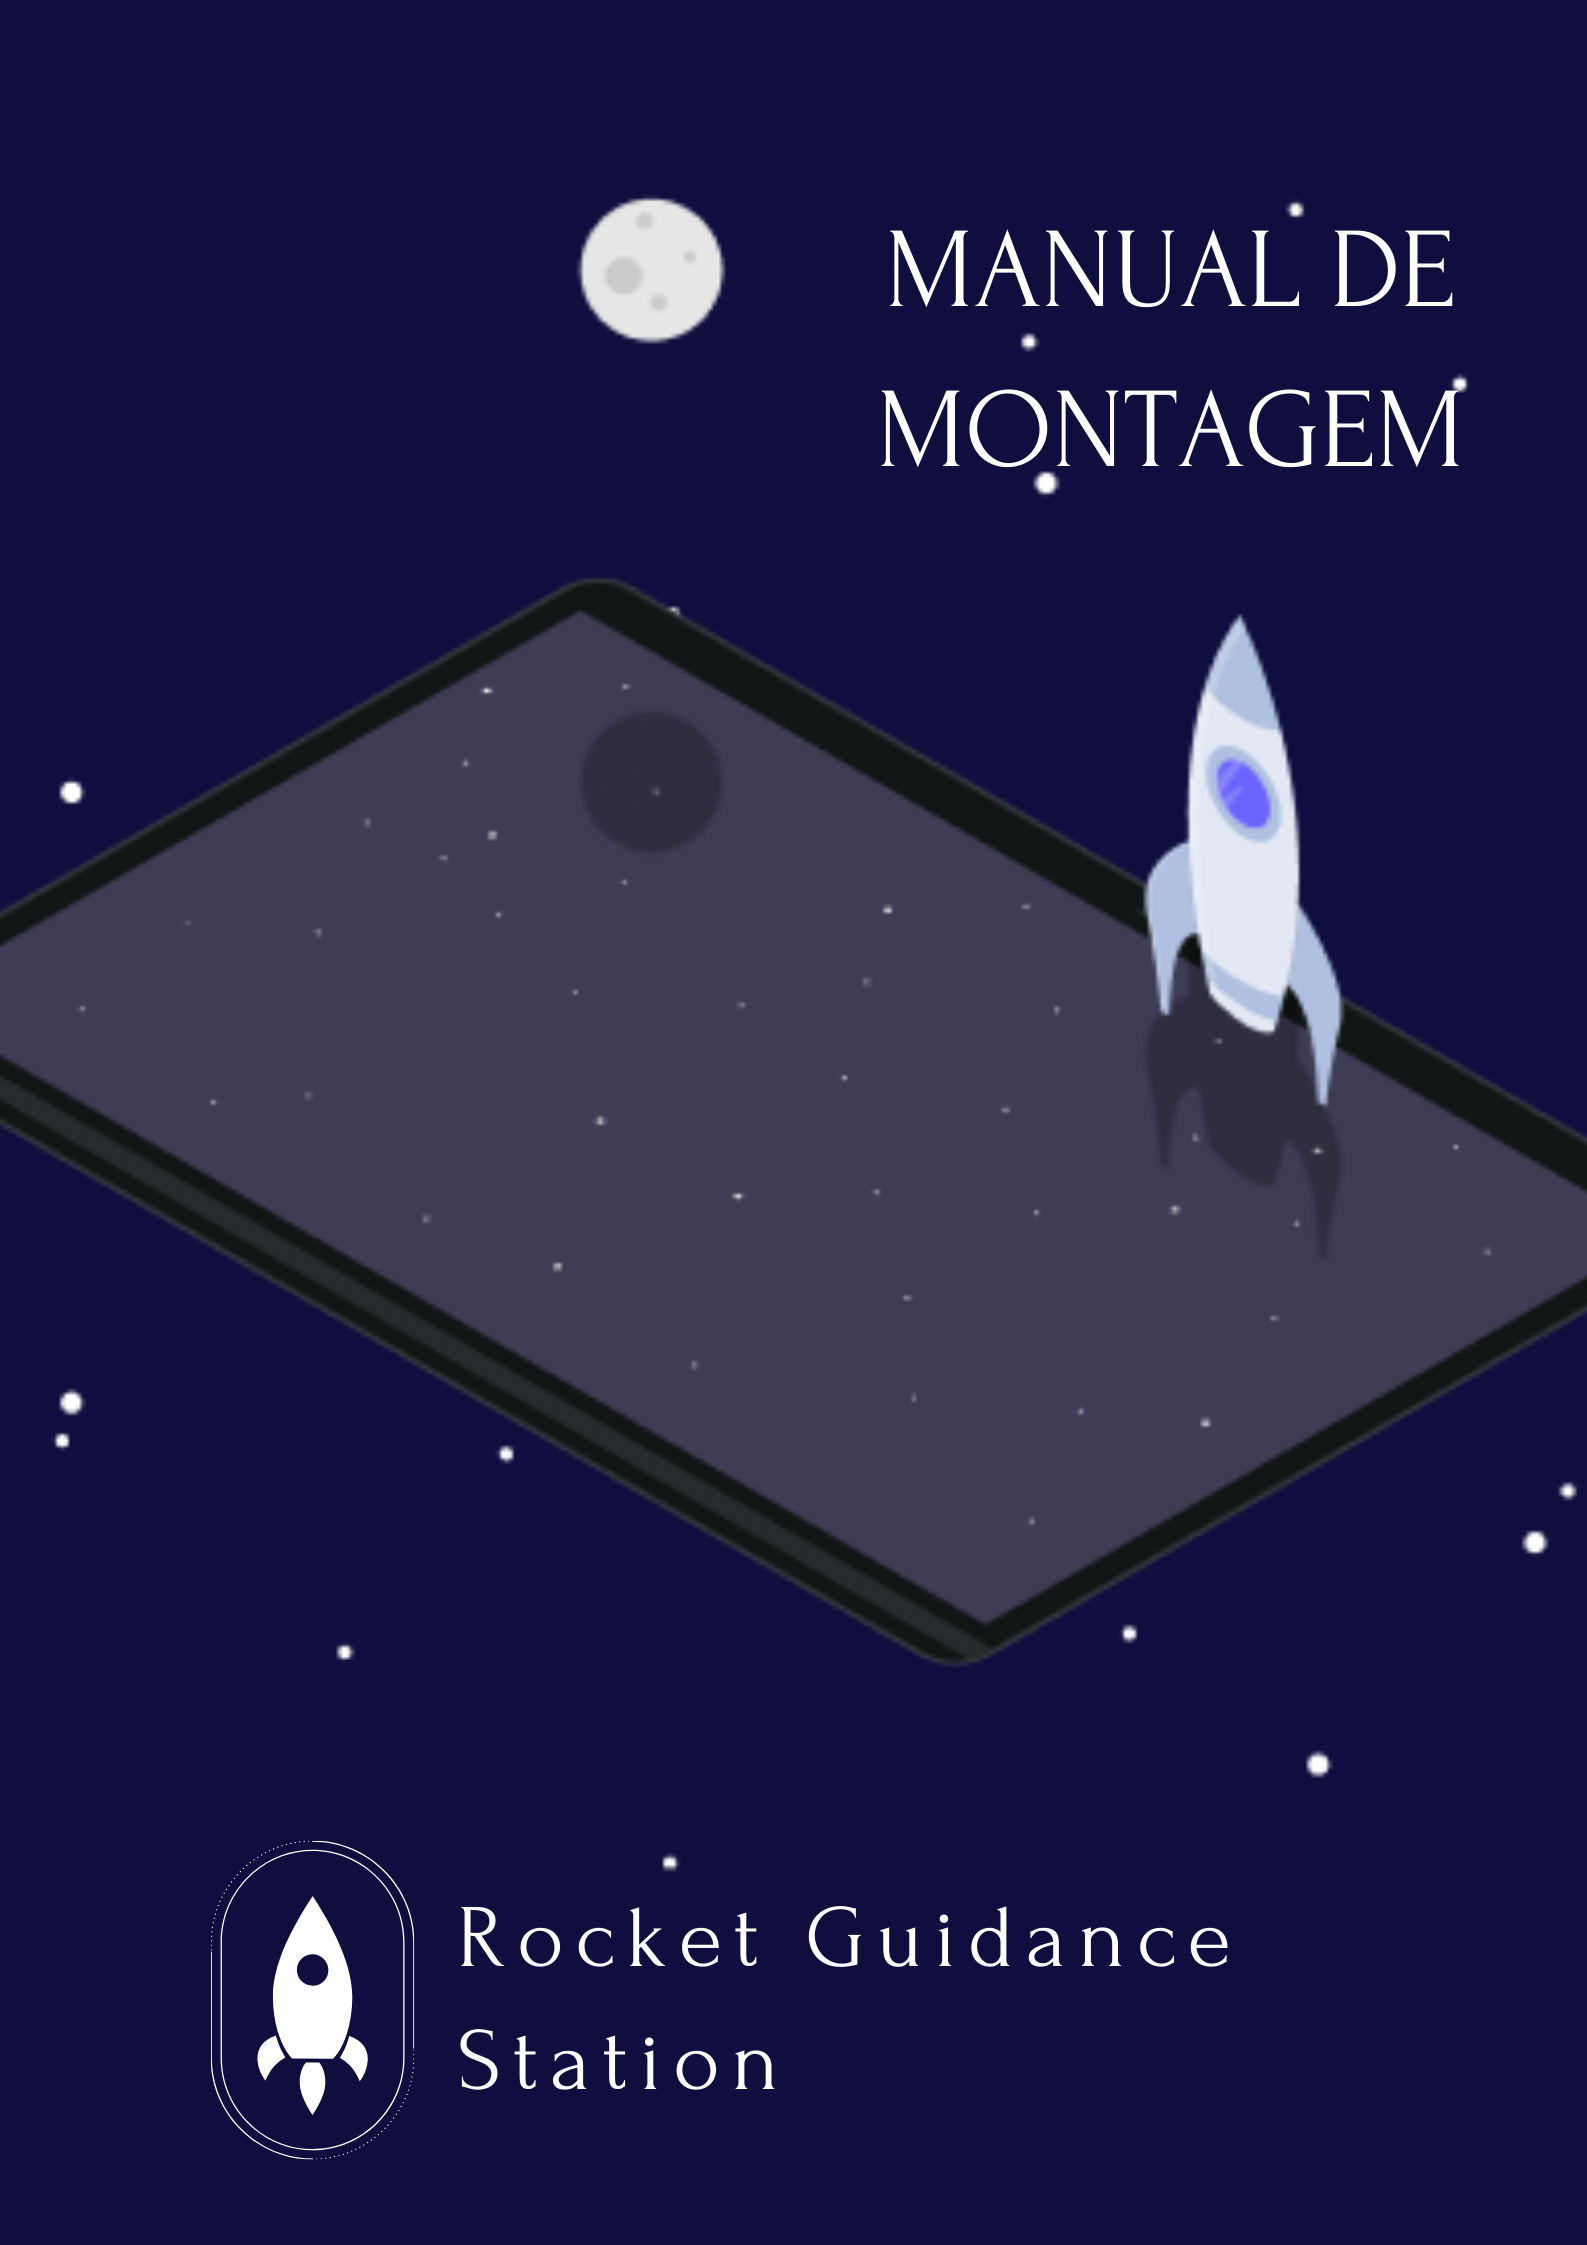
\includegraphics[width=\paperwidth\linewidth]{Figuras/capa.png}}} % Image background
\centering
\vspace*{11.3cm}
\par\normalfont\fontsize{35}{35}\sffamily\selectfont

\endgroup


%=========================================
\newpage{}
\thispagestyle {empty}

\vspace*{2cm}

\begin{center}

	\Large{\parbox{12cm}{
		\begin{raggedright}
		{\Large 
			Este manual foi elaborado pela equipe Rocket Guidance Station, a fim de elucidar o processo de construção e montagem do produto proposto. 
			\vspace*{1cm}
			
			Para tanto é necessário que leia-se atentamente todas as instruções de fabricação e montagem, para evitar acidentes ou a confecção errada do sistema apresentado.
			\vspace*{1cm}
			
			Qualquer contribuição ou crítica que possa melhorar a qualidade deste produto ou manual será bem-vinda pela equipe.
		}
	
		\vspace{.5cm}\hfill{Rocket Guidance Station}
		\end{raggedright}
	}
}
\end{center}

%\pdfbookmark[0]{\contentsname}{toc}
\tableofcontents
%\cleardoublepage

\newpage
\chapter{Montagem eletrônica}
%\section{Lista de Materiais}

%\begin{table}[H]
%\centering
%\begin{tabular}{|m{1.8cm} |m{9.2cm}|m{4cm}|}
%\hline
%\begin{center}Quantidade\end{center} & \begin{center}Componente\end{center} &\begin{center} Part Number\end{center} \\\hline
 %03&Lora Esp32 Sx1278 Com Display  Oled Wifi bluetooth 915mhz& Sx1278 \\\hline
 
%03 &  Conversor DC-DC Step Down-LM2596 (12~5V)
%& LM2596 \\\hline
  
%01& Módulo Gps  Gy-gps6m v2 & GPS NEO6M \\\hline
   
%03&LConector Borne KRE 2 Vias & KRE Kf301 \\\hline

%01&Sensor De Pressão e Temperatura BMP 280 & BST-BMP280-DS001-11 \\\hline

%01&Módulo Cartão de Memória MICRO SD CARD & B01IPCAP72 \\\hline

%01& Driver Motor Ponte H L298n & L298 \\\hline

%01&Módulo Conversor Nível Lógico 5V/3.3V -Bidirecional&  MOD-CXI2C \\\hline

%02& Sensor de Peso 50Kg Célula de Carga & SEN-10245\\\hline

%01&Módulo Hx711 Célula De Carga Balança 24 Bits & HX711 \\\hline

%14& porca de bronze espaçador hexagonal M5 X 12mm & -  \\\hline

%02 &  Módulo Relé 5V 2 Canais &   SRD-05VDC-SL-C \\\hline

%03 & Conector Jack J4 DC Fêmea &  Jack Fêmea  \\\hline

%02 & Conector Adaptador Plug P4 Macho com Borne &  P4 Macho F0503 \\\hline

%01 & Micro Usb V8 Macho & J5415\\\hline

%01 & Plug Hdmi Macho & Hdmi Macho \\\hline

%01 & NVIDIA Jetson Nano Developer Kit  & 945-13450-0000-100 \\\hline

%01 &Placa controladora   & PCB800099-V.9  \\\hline

%01 & Display LCD 9 polegadas  & Lcd 9 Polegadas TMOEC \\\hline

%01 & Mini  Teclado  slim  com  Touchpad & -  \\\hline

%01 & PCI- Base & -  \\\hline
%01 & PCI- Foguete & -  \\\hline
%01 & PCI- Maleta & -  \\\hline

%\end{tabular}
%\caption{Lista de componentes}
%\end{table}

\section{Ferramentas}

\par Para a soldagem dos componentes eletrônicos nas PCIs (Placas de Circuito Impresso), conexões dos fios com os módulos necessários e fixação da PCI na case de proteção ou outro local, é necessário o uso das seguintes ferramentas e acessórios:

\begin{itemize}
    \item Ferro de Solda ou Estação de Solda (15W-40W)
    \item Solda Estanho em fio 1mm
    \item Esponja metálica ou esponja convencional para limpeza da ponta de solda
    \item Lupa com suporte e pinça, para apoio e manuseio da PCI
    \item Sugador de solda
    \item Chave de fenda/phillips
    \item Alicate de corte pequeno
    \item Alicate de desencapar ou estilete
    \item Multímetro
\end{itemize}

\begin{center}
ATENÇÃO
\begin{figure}[H]
 \centering
 
\includegraphics[scale = 0.1]{Figuras/atenção.png}
\end{figure}
\end{center}

\par Os ferros de solda aquecem a temperaturas superiores a 400ºC. Usar um suporte para ferro de solda de boa qualidade é fundamental para não se acidentar e sofrer com queimaduras. Além disso, certifique-se de trabalhar em uma área bem ventilada ou use um extrator de fumaça ou exaustor de fumaça. Os vapores do fluxo são tóxicos. Leia atentamente as instruções deste manual. Ao soldar, utilize Equipamentos de Proteção Individual (EPIs), tais como, óculos de segurança e luvas de segurança. Mantenha todo o cabelo, roupas folgadas e joias protegidos e fora do caminho de suas ferramentas. Se a solda que você estiver usando contiver chumbo, lave as mãos após concluir o trabalho.


\subsection{Boas práticas}

\subsection{Manuseio da PCB e componentes eletrônicos}
\PAR É de bom grado ter alguns cuidados ao montar e manter em boas condições as placas de circuito impresso-PCI que estão sujeito a vários fatores de risco como:
\begin{itemize}
\item \textbf{Mecânicos:}
\begin{itemize}
\item Vibrações
\item flexões nas PCI 
\item choques mecânicos
\end{itemize}
\end{itemize}

\begin{itemize}
\item \textbf{Ambientais:}
\begin{itemize}
\item Umidade em excesso
\item Contaminantes pelo ar 
\item Excesso de luz solar
\end{itemize}
\end{itemize}

\begin{itemize}
\item \textbf{Eletrostático:}
\begin{itemize}
\item Descargas elétricas produzidas por atrito e contato humano sem devidos cuidados
\end{itemize}
\end{itemize}

\par {\textbf{Alguns cuidados devem ser tomados:}}

\begin{itemize}
\item Evitar tocar em partes metálicas dos componentes e nos conectores e minimizar o manuseio o máximo possível evitando danos mecânicos;
\item É recomendável segurar a placa de forma a não tocar nas suas trilhas preferível que o manuseamento da mesma seja feito de forma que a pessoa segura a placa pelas suas bordas/ laterais;  

\item Nunca flexione a placa ou utilize de muita força ao manuseá-la pode acarretar em rompimento das trilhas,rompimentos de ligações  de encaixe;

\item Não deixe os equipamentos perto de recipientes com água e nem molhe-os.
\end{itemize}

\subsection{Soldagem dos componentes}

\PAR Para obter um circuito eletrônico confiável é necessário não somente que o circuito impresso tenha qualidade, mas também que as junções elétricas feitas entre as ilhas da PCI e os terminais dos componentes possuem sejam de qualidade.

Ao realizar a soldagem, a ilha de cobre da PCI e o terminal do componente devem ser aquecidos a uma temperatura superior à de fusão da solda. A solda deve ser aplicada apenas após o aquecimento para que se evite a solda fria. A solda deve ser aplicada à junção. Se a solda for aplicada à ponta do ferro de soldar, o fluxo contido na solda será evaporado sem que a oxidação seja removida, perdendo o seu efeito.

Para obter uma boa solda, esta deve ter aparência brilhante e regular, com uma superfície suavemente côncava, vide Figura \ref{fig:Solda Ideal}. Superfícies com aparência opaca e convexa são características de solda fria.

\begin{figure}[H]
  \centering
  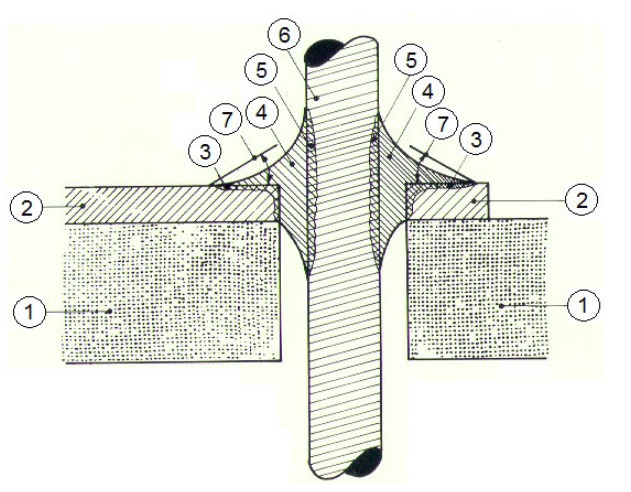
\includegraphics[width=\textwidth]{Figuras/soldagem_ideal.jpeg}
  \caption{Partes de uma PCI e uma soldagem eficiente.} 
 { \footnotesize FONTE (ADAPTADO): "MCE - Montagem de Circuitos Eletrônicos". 
 Wilson Carvalho - ETEC ALBERT EINSTEIN (2014)} 
  \label{fig:Solda Ideal}
\end{figure}

A Figura \ref{fig:Solda Ideal} apresenta os pontos que caracterizam uma solda eficiente. Onde cada ponto é identificado da seguinte forma:

\begin{enumerate}
    \item Substrato da PCI
    \item Camada de cobre
    \item Liga de solda e pista de cobre (somente algumas moléculas de espessura)
    \item Solda
    \item Liga de solda e terminal do componente
    \item Terminal do componente
    \item Ângulo máximo entre a solda e a pista impressa (inferior a 30°)
\end{enumerate}

\newpage

\chapter{Placas de Circuito Impresso}

\section{Confecção das placas de circuito impresso}

\par Para a confecção das placas de circuito impresso foram gerados os arquivos Gerber de cada placa de circuito impresso, sendo gerado um arquivo em formato ZIP disponíveis em Arquivos Gerber sendo fabricadas com 2 Layers com a placa contendo uma espessura de $1.6 mm$ e peso de cobre de $1 oz$. Para a visualização dos arquivos Gerber é necessário a utilização de um programa de prototipagem de placas de circuito impresso ou um visualizador desse tipo de arquivo disponível para download no site do programa utilizado para o projeto EasyEda como pode se observado na figura \ref{fig:Gerber}.
\par Link download arquivos Gerber: \href {https://drive.google.com/drive/folders/1P1pQGE_zuSLOB5qd8zfESWqLDwtyoRKd?usp=sharing}{aqui}
\par Link download do programa vizualizador: \href{https://sourceforge.net/projects/gerbv/files/}{aqui} 

\begin{figure}[H]
  \centering
  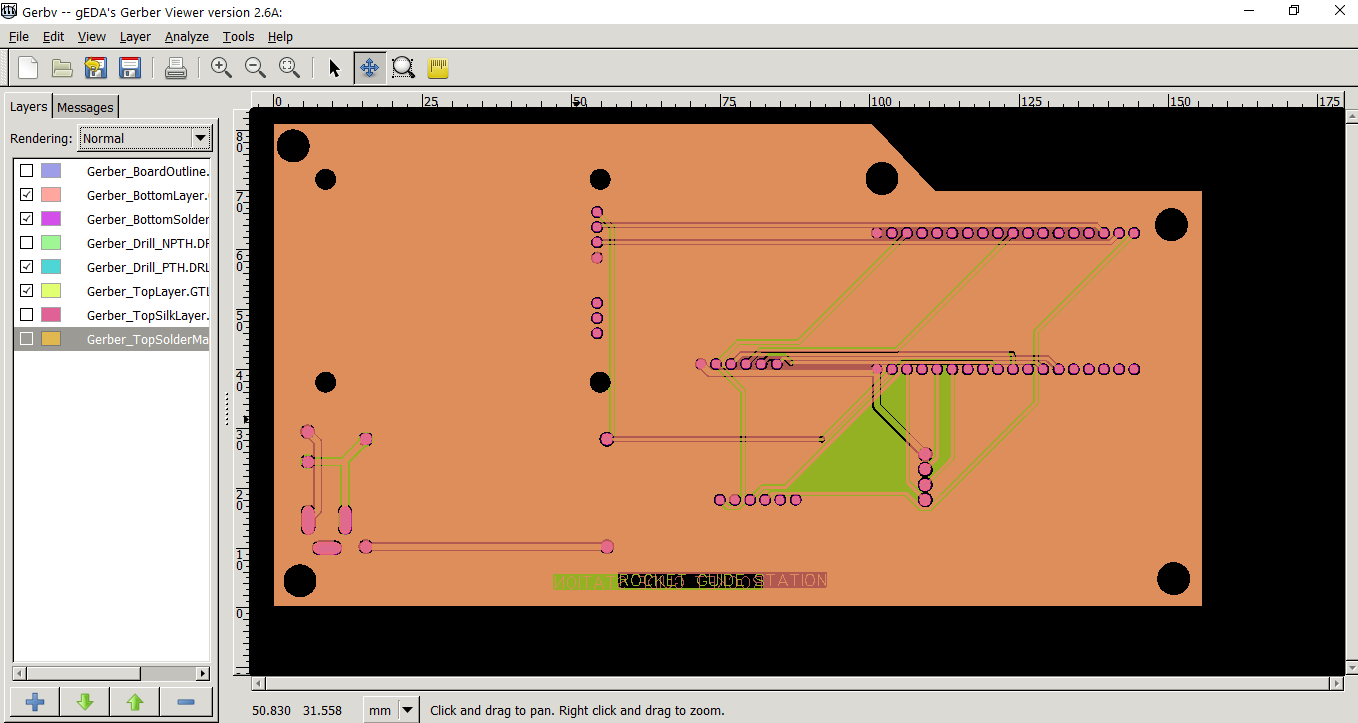
\includegraphics[scale=0.3]{Figuras/pci fabric/imagem de fabicação.png}
  \caption{Programa visualizador do Gerber.}
  \label{fig:Gerber}
\end{figure}

\subsection{Placa de Circuito Impresso-Foguete}
\par Na figura \ref{fig:Gerber da PCI-Foguete} se encontra parte do arquivo Gerber para a fabricação da PCI do foguete e na \ref{fig: PCI-Foguete} se encontra o projeto final de como deve ficar apos a fabricação da mesma.

\begin{figure}[H]
  \centering
  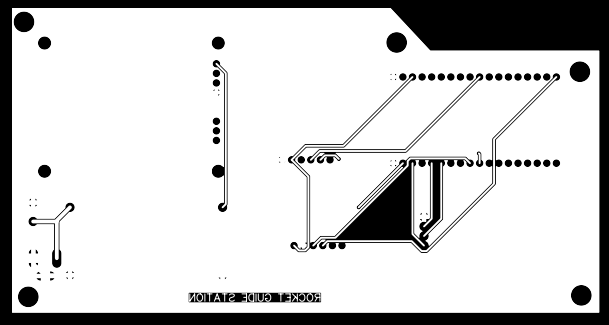
\includegraphics[scale=0.4]{Figuras/pci fabric/gerber foguete bottomlayer.png}
    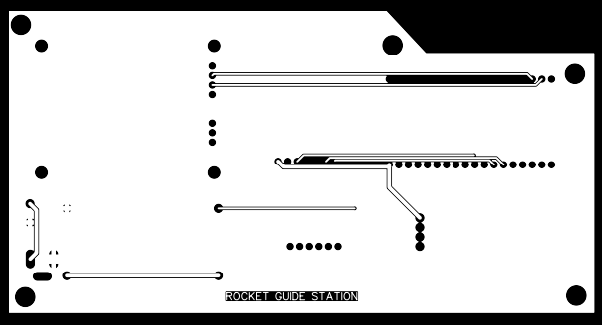
\includegraphics[scale=0.4]{Figuras/pci fabric/gerber foguete toplayer.png}
  \caption{Gerber da PCI-Foguete.}
  \label{fig:Gerber da PCI-Foguete}
\end{figure}

\begin{figure}[H]
  \centering
  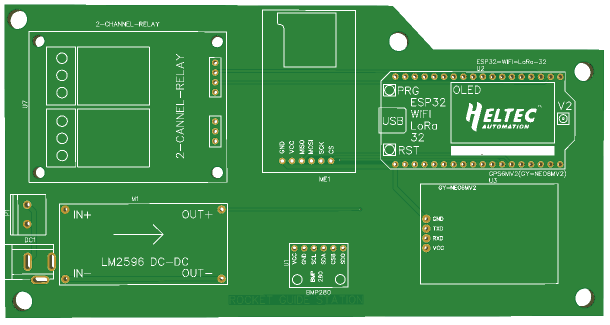
\includegraphics[scale=0.4]{Figuras/pci fabric/foguete_top.png}
    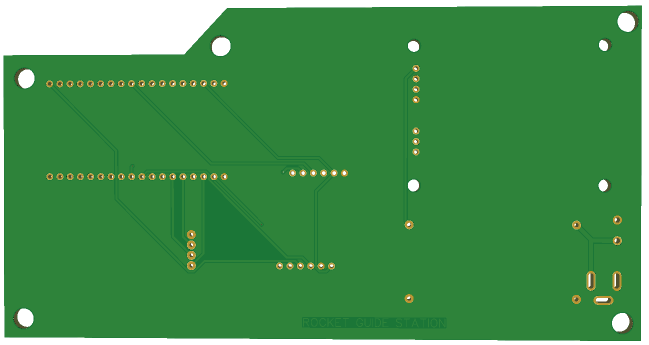
\includegraphics[scale=0.4]{Figuras/pci fabric/foguete_bottom.png}
  \caption{ PCI-Foguete.}
  \label{fig: PCI-Foguete}
\end{figure}

\subsection{Placa de Circuito Impresso-Base de Lançamento}

\par Na figura \ref{fig:Gerber da PCI-Base} se encontra parte do arquivo Gerber para a fabricação da PCI do foguete e na \ref{fig: PCI-Base} se encontra o projeto final de como deve ficar apos a fabricação da mesma.



\begin{figure}[H]
  \centering
  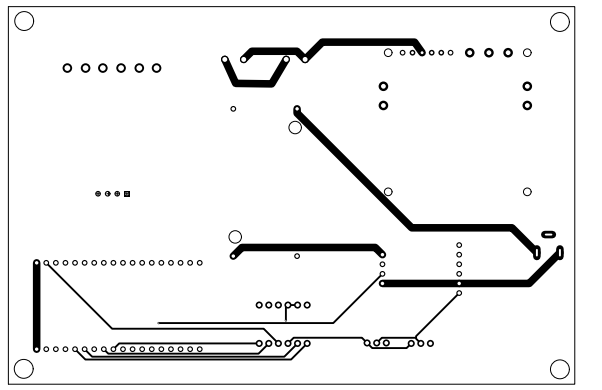
\includegraphics[scale=0.4]{Figuras/pci fabric/gerber base toplayer.png}
    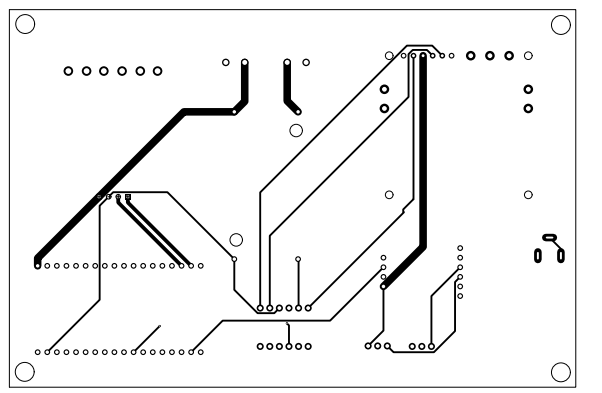
\includegraphics[scale=0.4]{Figuras/pci fabric/gerber base bottom layer.png}
  \caption{Gerber da PCI-Base.}
  \label{fig:Gerber da PCI-Base}
\end{figure}

\begin{figure}[H]
  \centering
  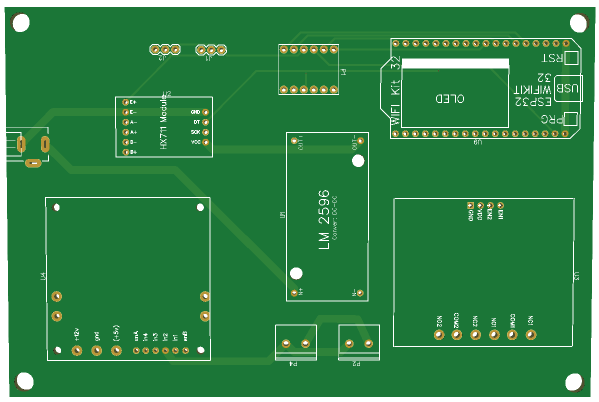
\includegraphics[scale=0.4]{Figuras/pci fabric/BASE_TOP.png}
    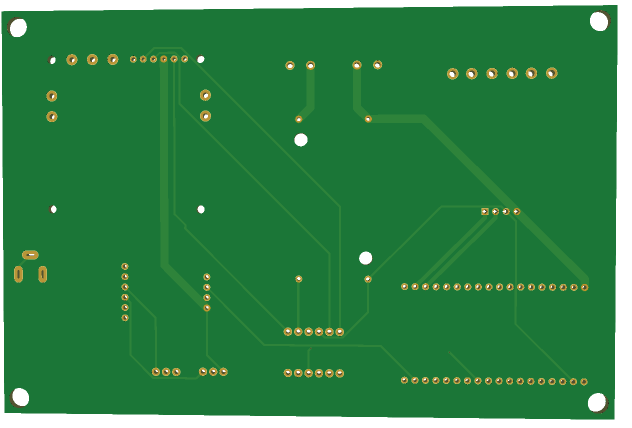
\includegraphics[scale=0.4]{Figuras/pci fabric/BASE_BOTTOM.png}
  \caption{ PCI-Base.}
  \label{fig: PCI-Base}
\end{figure}



\subsection{Placa de Circuito Impresso-Maleta Interface do Usuário}

\par Na figura \ref{fig:Gerber da PCI-Maleta} se encontra parte do arquivo Gerber para a fabricação da PCI do foguete e na \ref{fig: PCI-Maleta} se encontra o projeto final de como deve ficar apos a fabricação da mesma.

\begin{figure}[H]
  \centering
  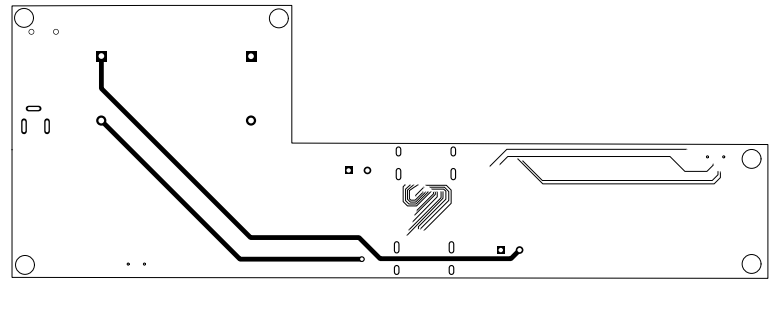
\includegraphics[scale=0.35]{Figuras/pci fabric/gerber maleta bottom layer.png}
    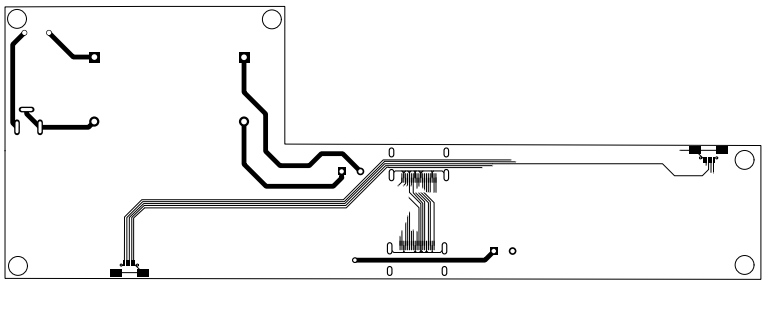
\includegraphics[scale=0.35]{Figuras/pci fabric/gerber maleta toplayer.png}
  \caption{Gerber da PCI-Maleta.}
  \label{fig:Gerber da PCI-Maleta}
\end{figure}


\begin{figure}[H]
  \centering
  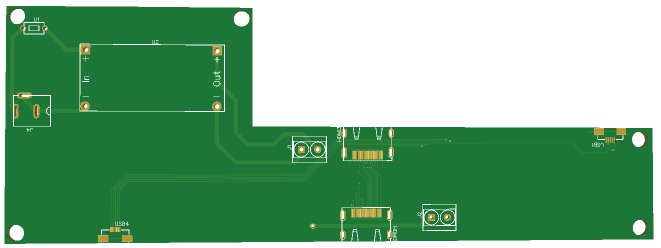
\includegraphics[scale=0.4]{Figuras/pci fabric/maleta_top.png}
    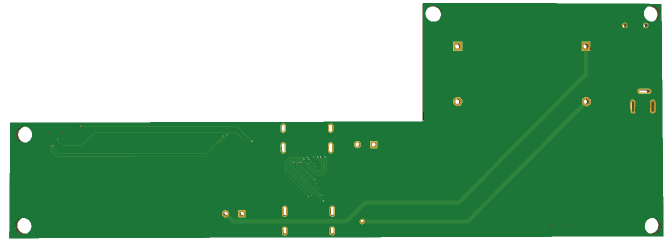
\includegraphics[scale=0.4]{Figuras/pci fabric/maleta_bottom.png}
  \caption{PCI-Maleta.}
  \label{fig: PCI-Maleta}
\end{figure}

\section{Instruções de Montagem das PCI's}
\par A montagem correta das placas é de suma importância para o correto funcionamento do hardware do projeto, siga os passos a seguir para garantir a correta montagem das placas de circuito impresso.
\begin{center}
ATENÇÃO
\begin{figure}[H]
  \centering
  
\includegraphics[scale = 0.1]{Figuras/atenção.png}
\end{figure}
\end{center}



\subsection{Placas de Circuito Impresso-Base de lançamento}
\subsubsection{Lista de Materiais}

\par Primeiramente é necessário ter em mão todos os componentes para sua montagem \ref{fig:Lista de materiasi base}.

\begin{table}[H]
\centering
\begin{tabular}{|m{1.9cm} |m{1.8cm} |m{7.3cm}|m{4cm}|}
\hline
\begin{center}Identificador\end{center} &\begin{center} Quantidade\end{center} & \begin{center}Componente\end{center} &\begin{center} Part Number\end{center} \\\hline
A&01 & PCI- Base & -  \\\hline
B &01&Lora Esp32 Sx1278 Com Display  Oled Wifi bluetooth 915mhz& Sx1278 \\\hline
 
C&01 &  Conversor DC-DC Step Down-LM2596 (12~5V)
& LM2596 \\\hline

D&01&Módulo Conversor Nível Lógico 5V/3.3V -Bidirecional&  MOD-CXI2C \\\hline

E&01&Módulo Hx711 Célula De Carga Balança 24 Bits & HX711 \\\hline

F&01& Driver Motor Ponte H L298n & L298 \\\hline

G&01 &  Módulo Relé 5V 2 Canais &   SRD-05VDC-SL-C \\\hline

H &02& Sensor de Peso 50Kg Célula de Carga & SEN-10245\\\hline

I&01 & Conector Jack J4 DC Fêmea &  Jack Fêmea  \\\hline

J&02&LConector Borne KRE 2 Vias & KRE Kf301 \\\hline

K&04&Parafuso Máquina Cabeça Chata Phillips M5 X 20mm &  Phillips M5 X 20mm \\\hline

L&04& porca de bronze espaçador hexagonal M5 X 12mm & -  \\\hline

\end{tabular}
\caption{Lista de componentes}
\end{table}


\subsubsection{Instruções}

\begin{figure}[H]
  \centering
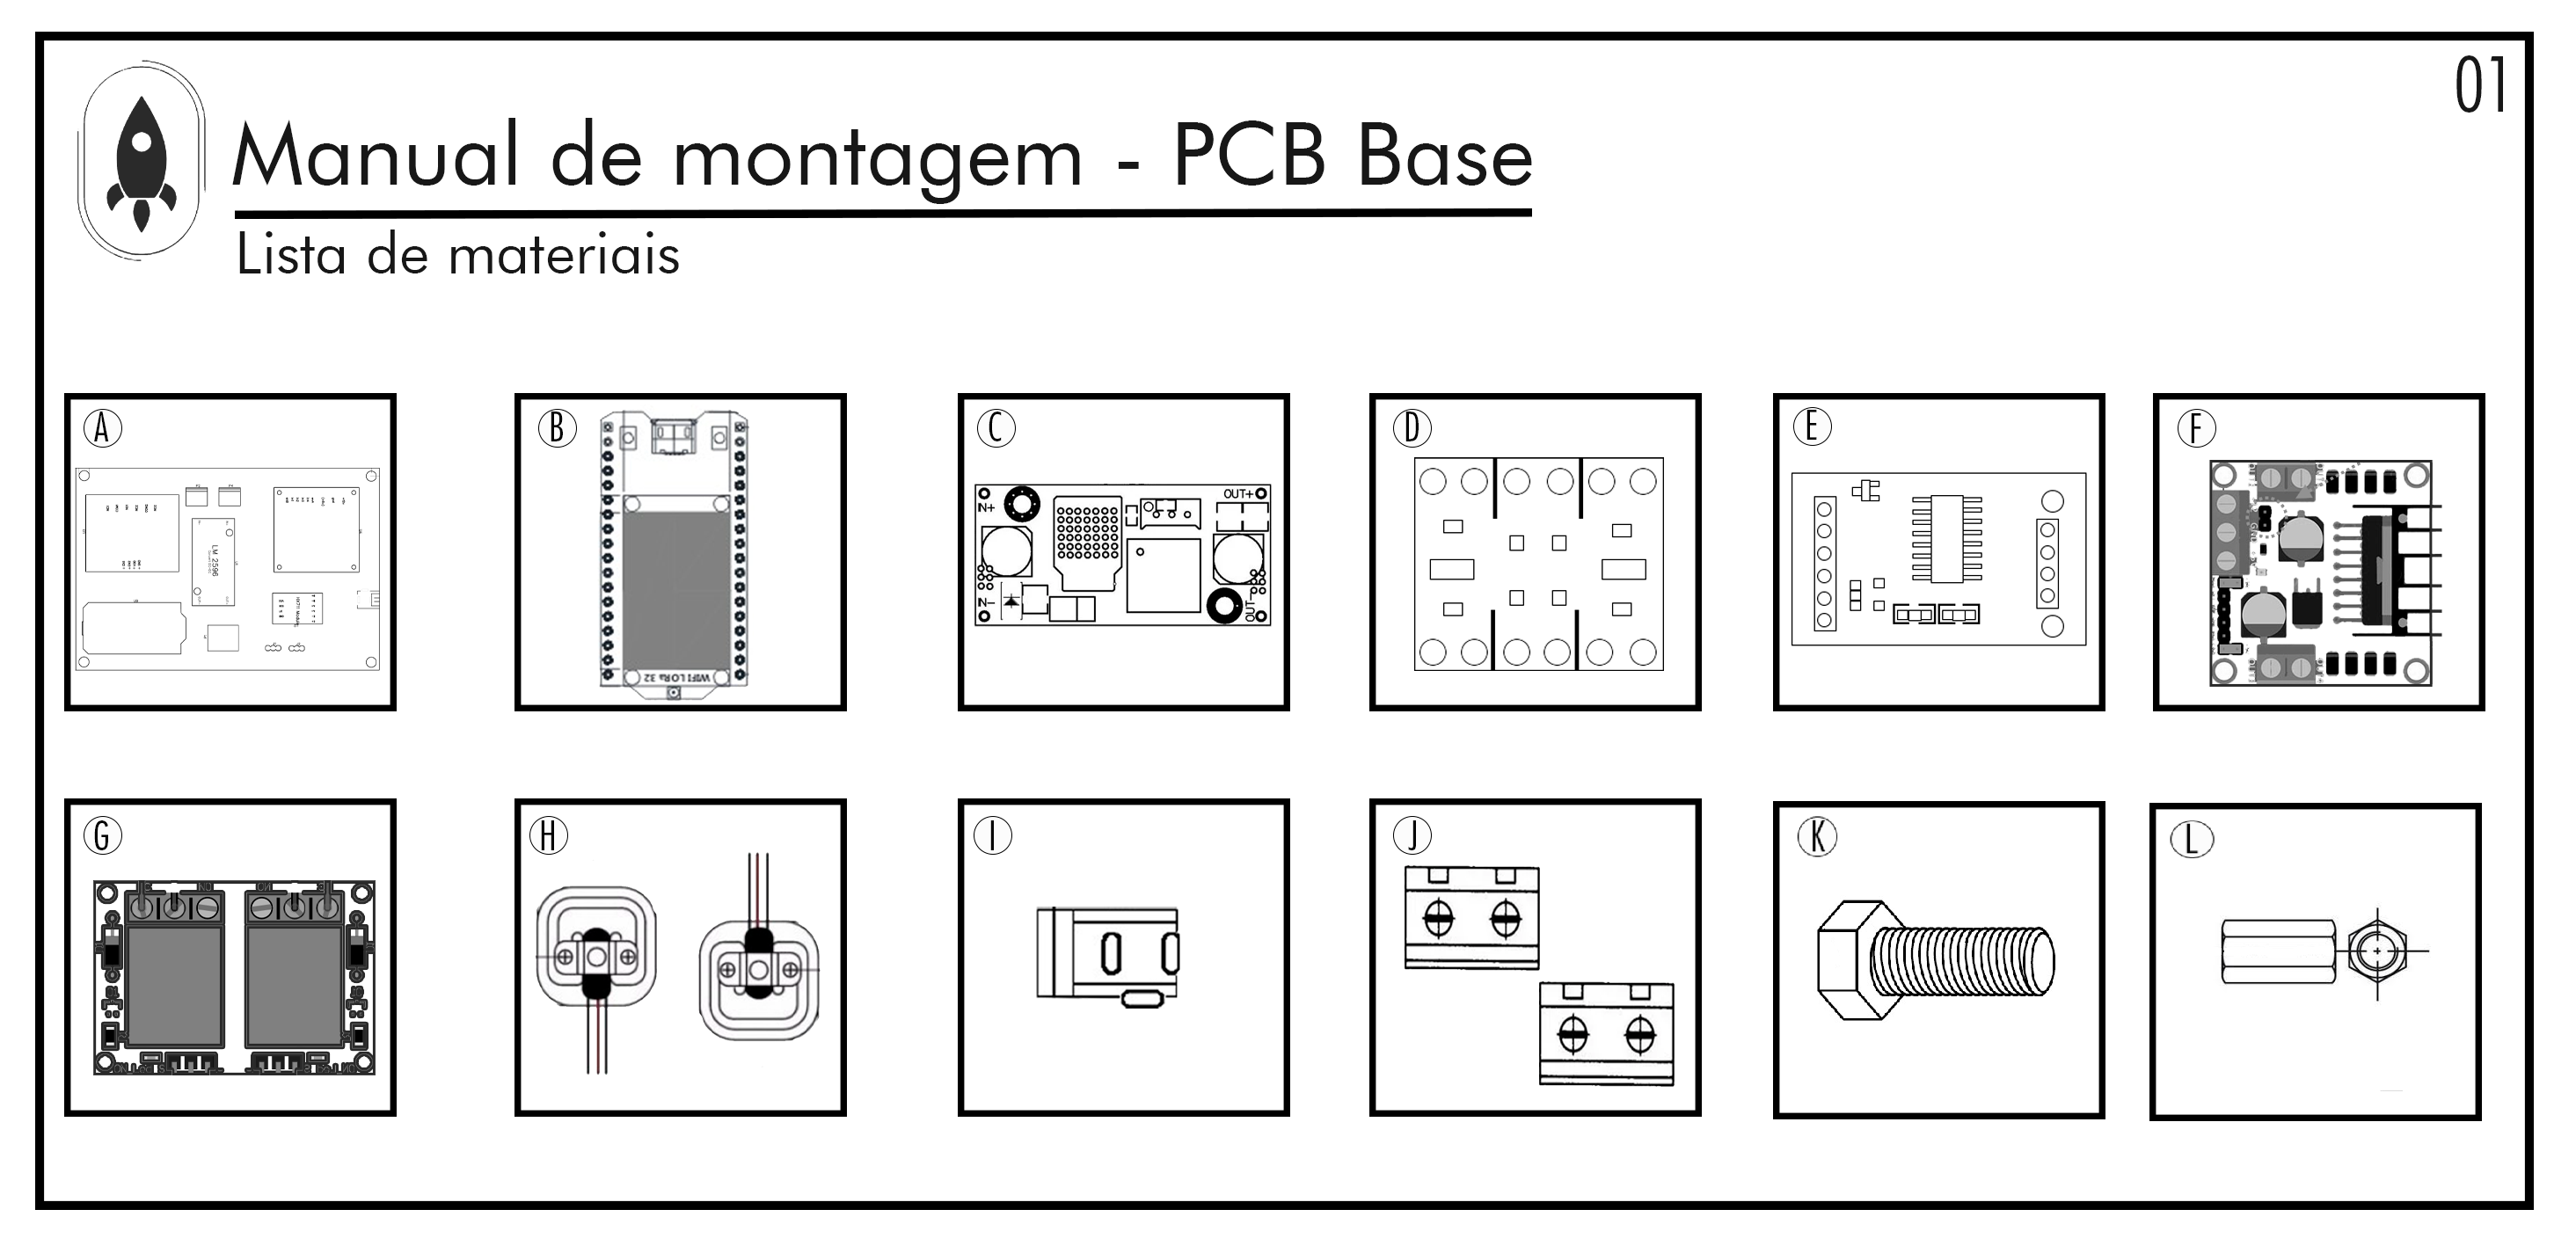
\includegraphics[width=\textwidth]{Figuras/BASE/Pg-01---PL-03.png}
  \caption{Lista de Materiais.} 
 %{ \footnotesize Fonte: Autores} 
 \label{fig:Lista de materiasi base}
 \end{figure}


 \par Com todos os componentes em mãos, pegue componente 'A'(PCI-BASE) prepare-a para soldagem dos componentes passando uma fina camada de solda nos pads da PCI.

\begin{figure}[H]
  \centering
  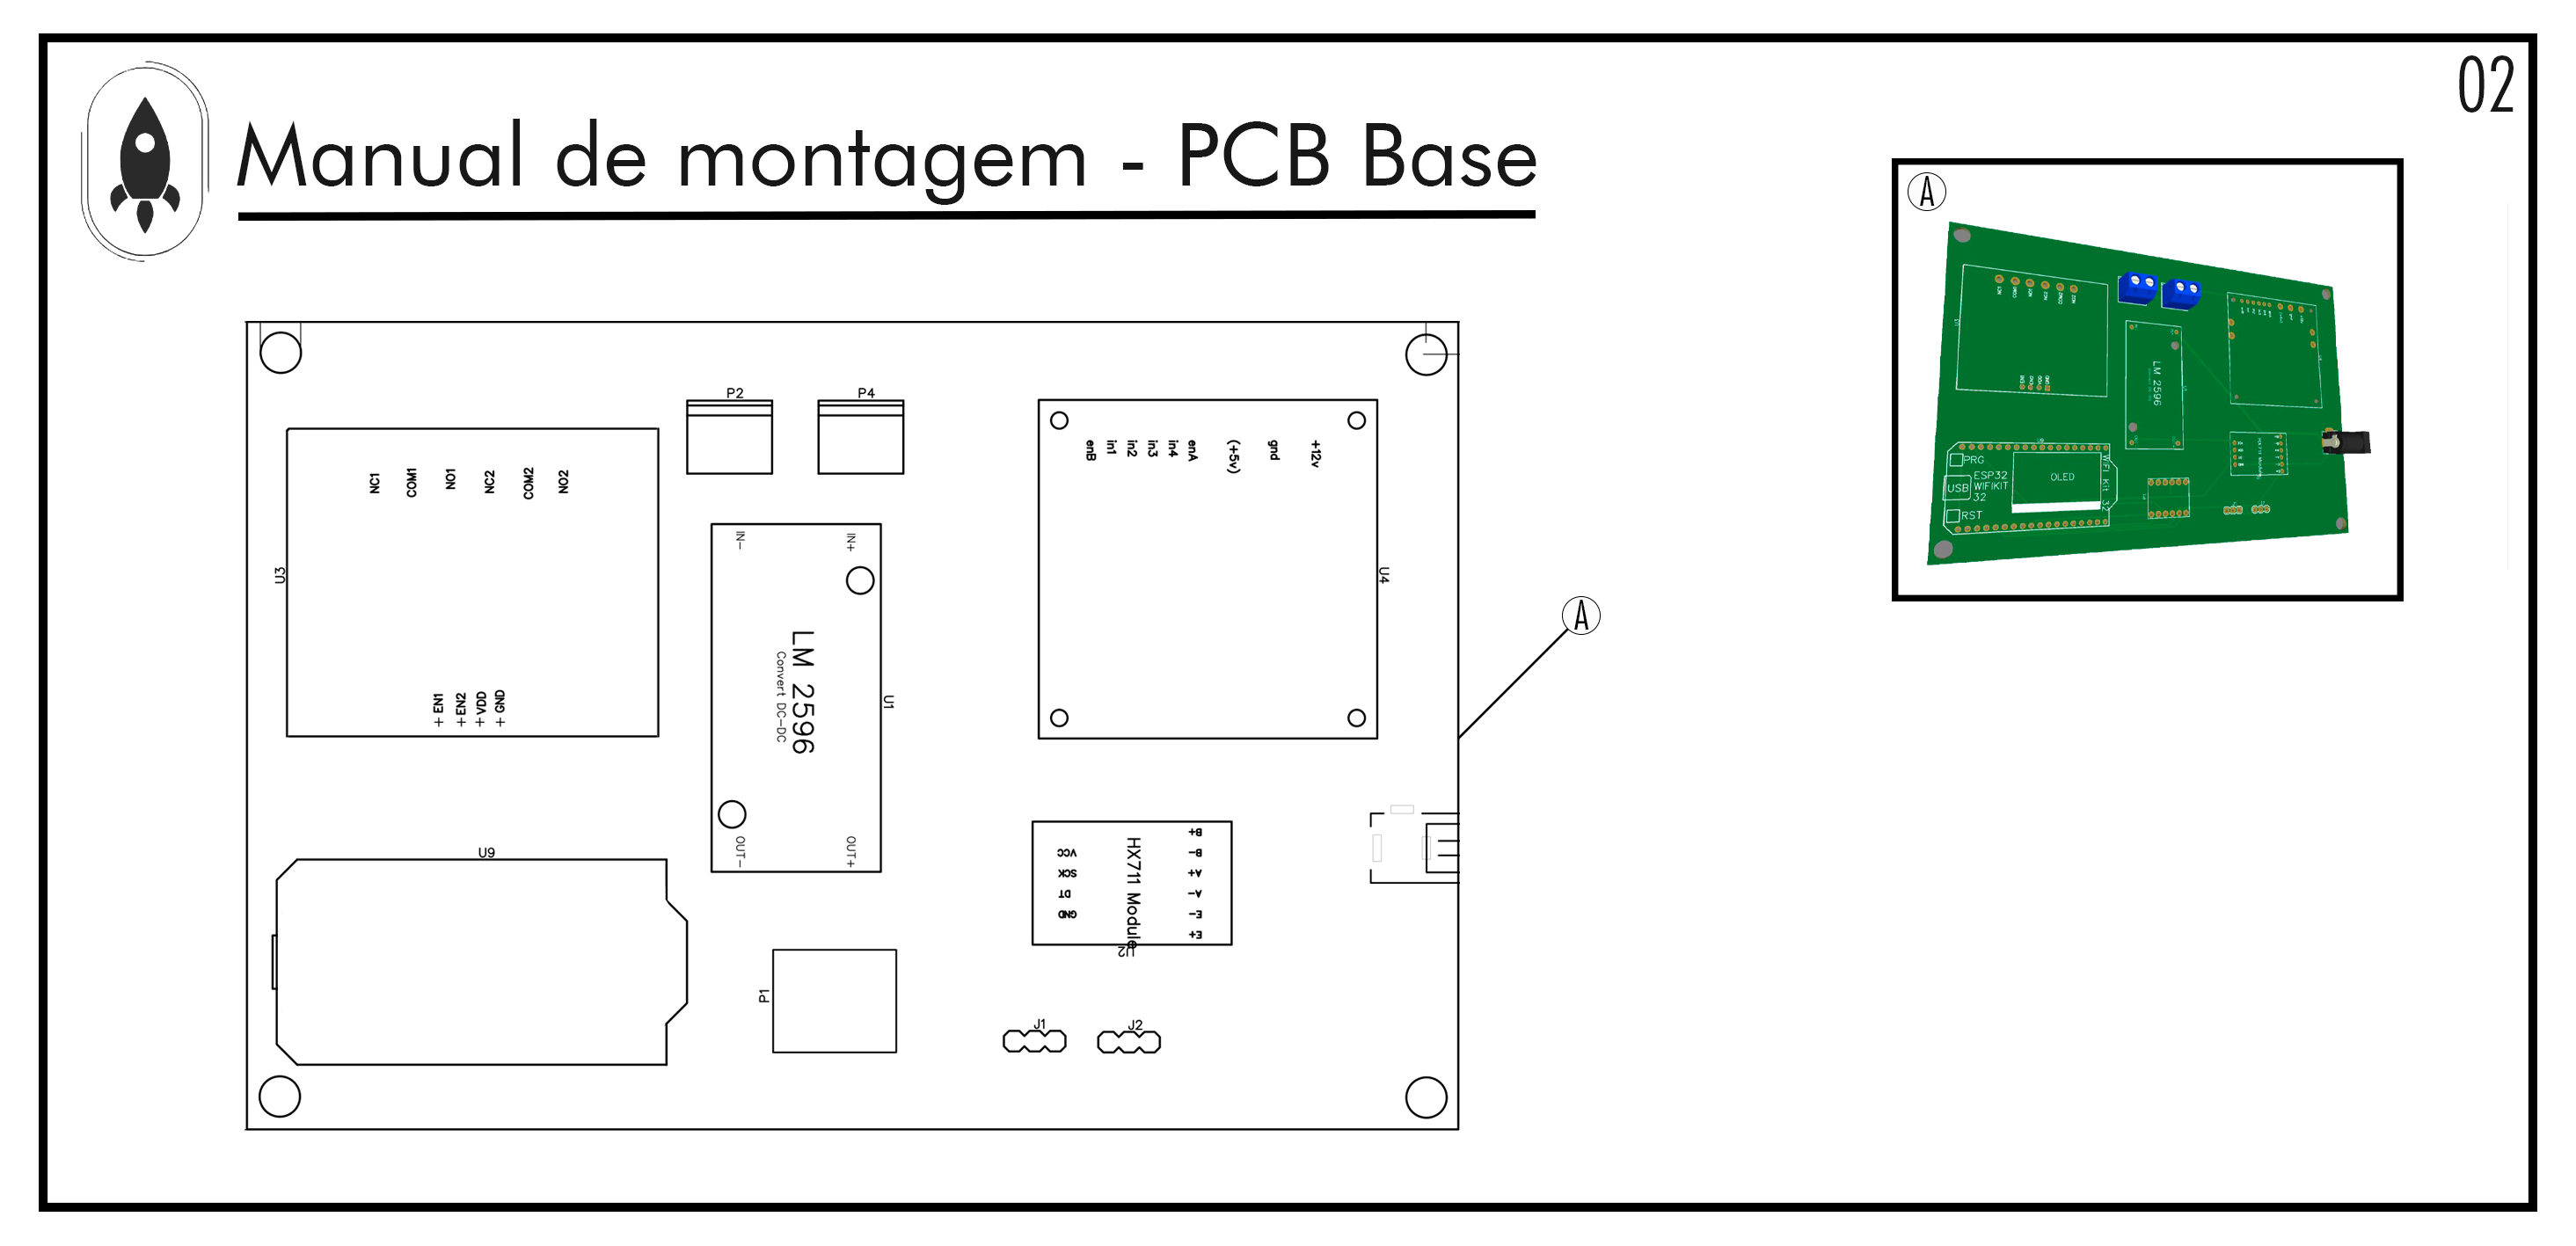
\includegraphics[width=\textwidth]{Figuras/BASE/Pg-02---PL-03.png}
  \caption{PCI da Base.}
 %{ \footnotesize Fonte: Autores} 
  \label{fig:PCIBASE}
\end{figure}

\newpage
\par Pegue o componente 'B'(ESP32 LoRa WiFi), encaixe-a na posição mostrada \ref{fig:PCIBASE LORA} e solde junto a placa.
\begin{figure}[H]
  \centering
  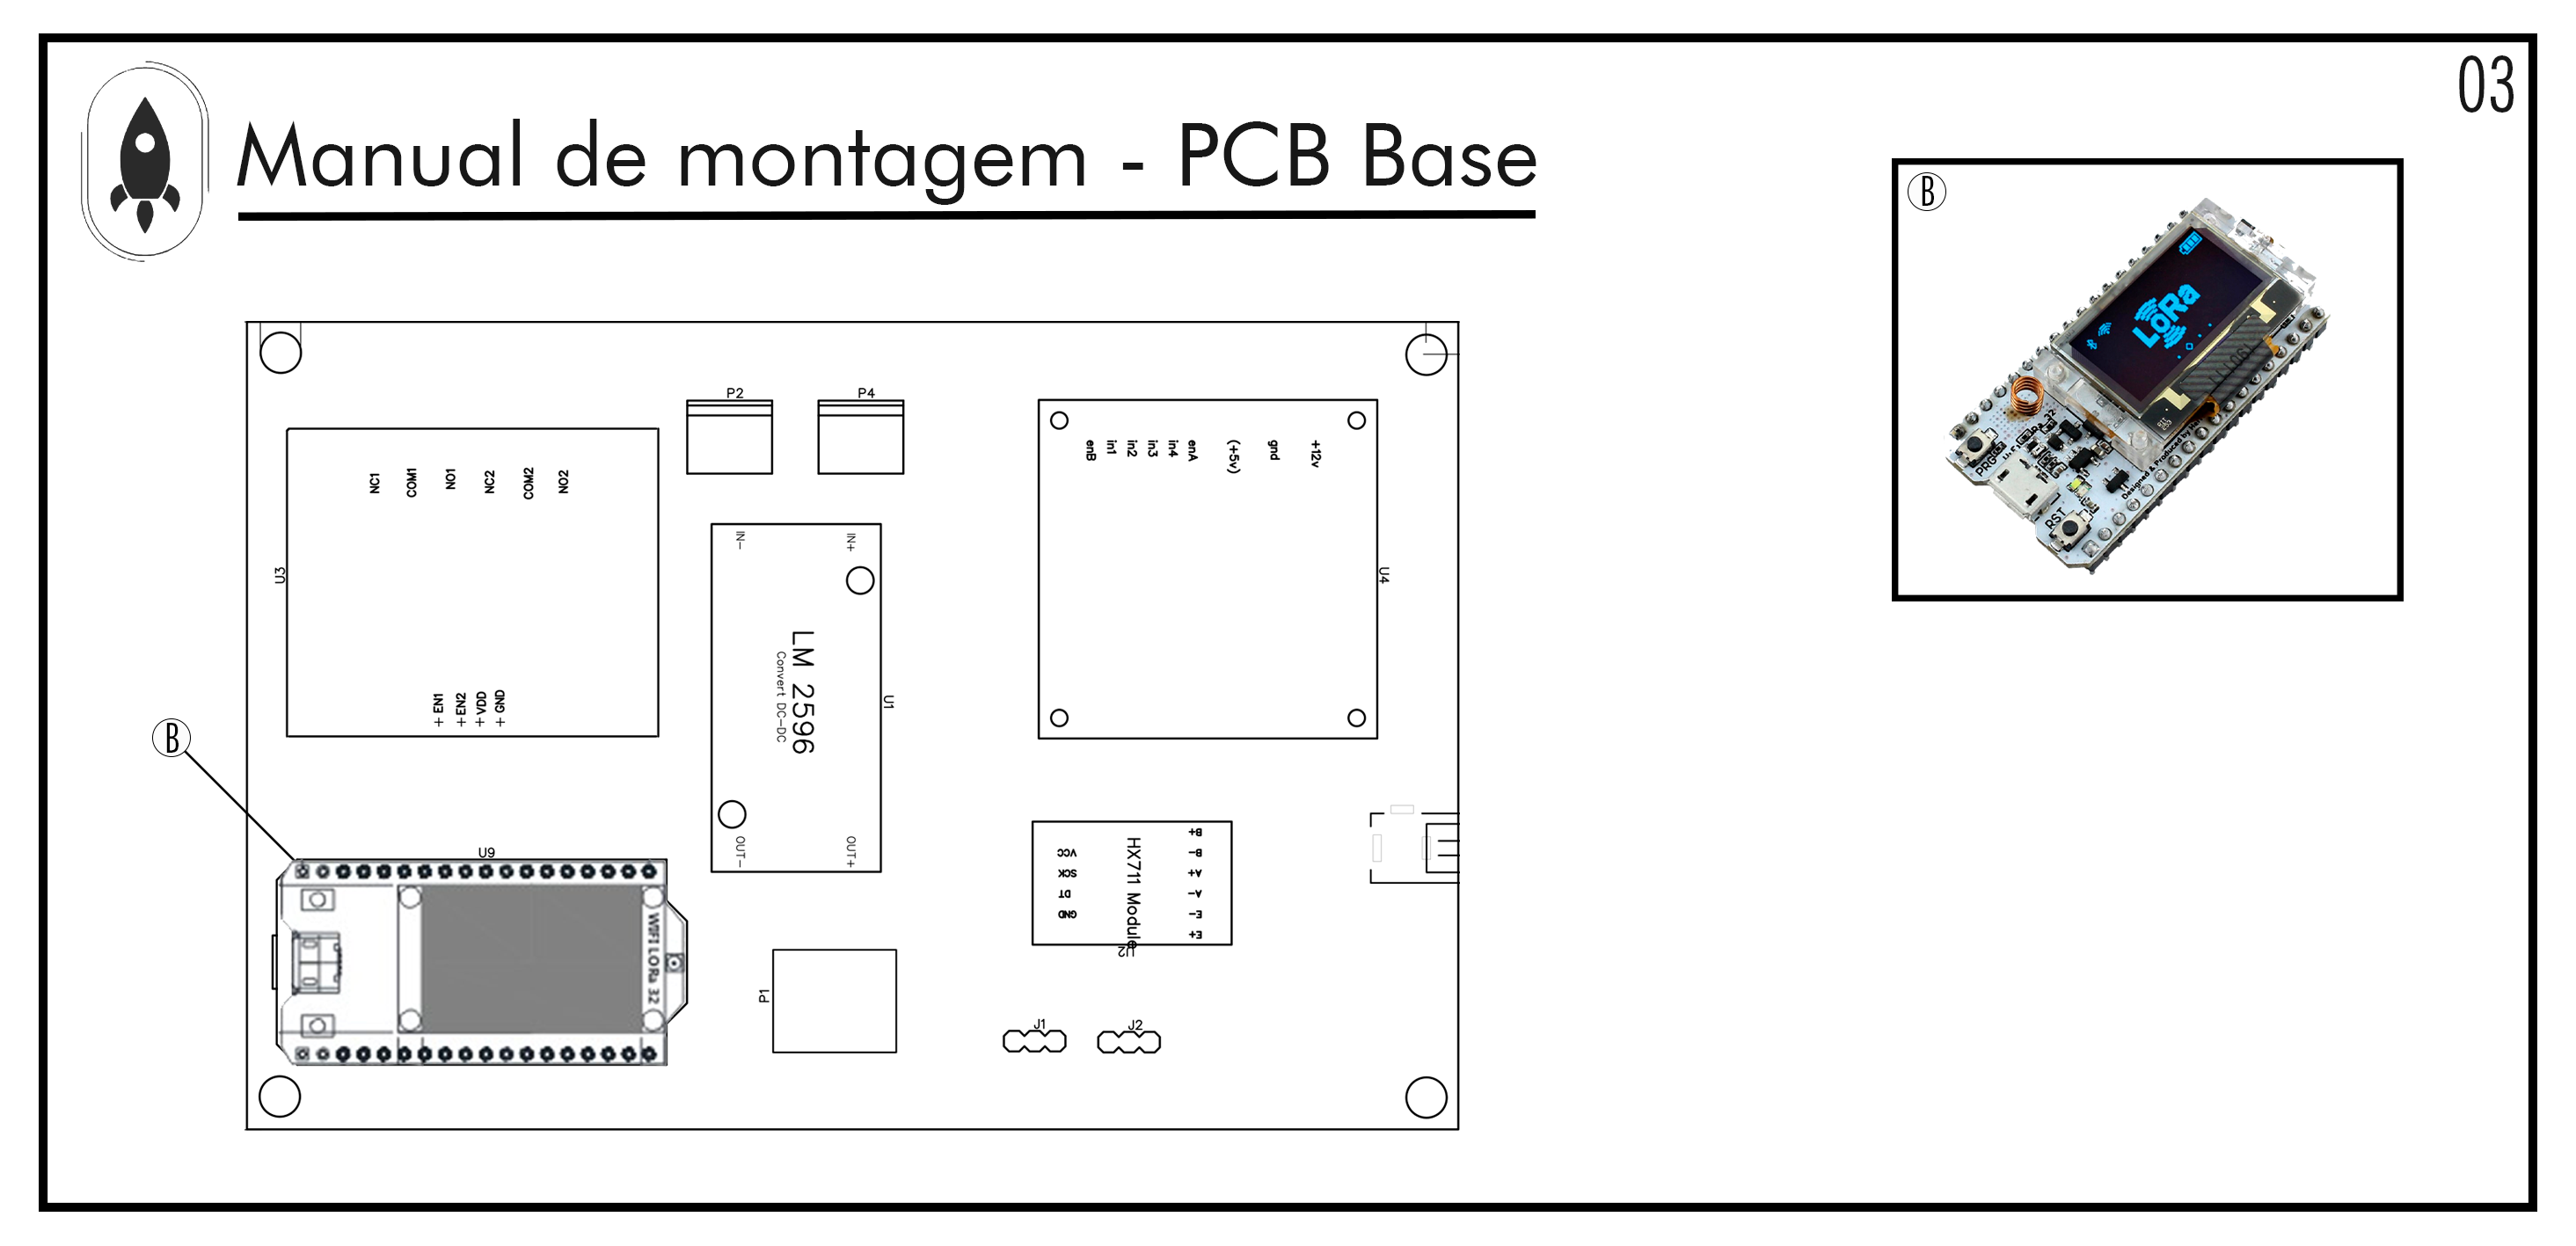
\includegraphics[width=\textwidth]{Figuras/BASE/Pg-03---PL-03.png}
  \caption{ESP32 WiFi Lora.}
 %{ \footnotesize Fonte: Autores} 
  \label{fig:PCIBASE LORA}
\end{figure}


\par Pegue o componente 'C'(LM2596), encaixe-a na posição mostrada \ref{fig:PCIBASE LM2596} e solde junto a placa.
\begin{figure}[H]
  \centering
  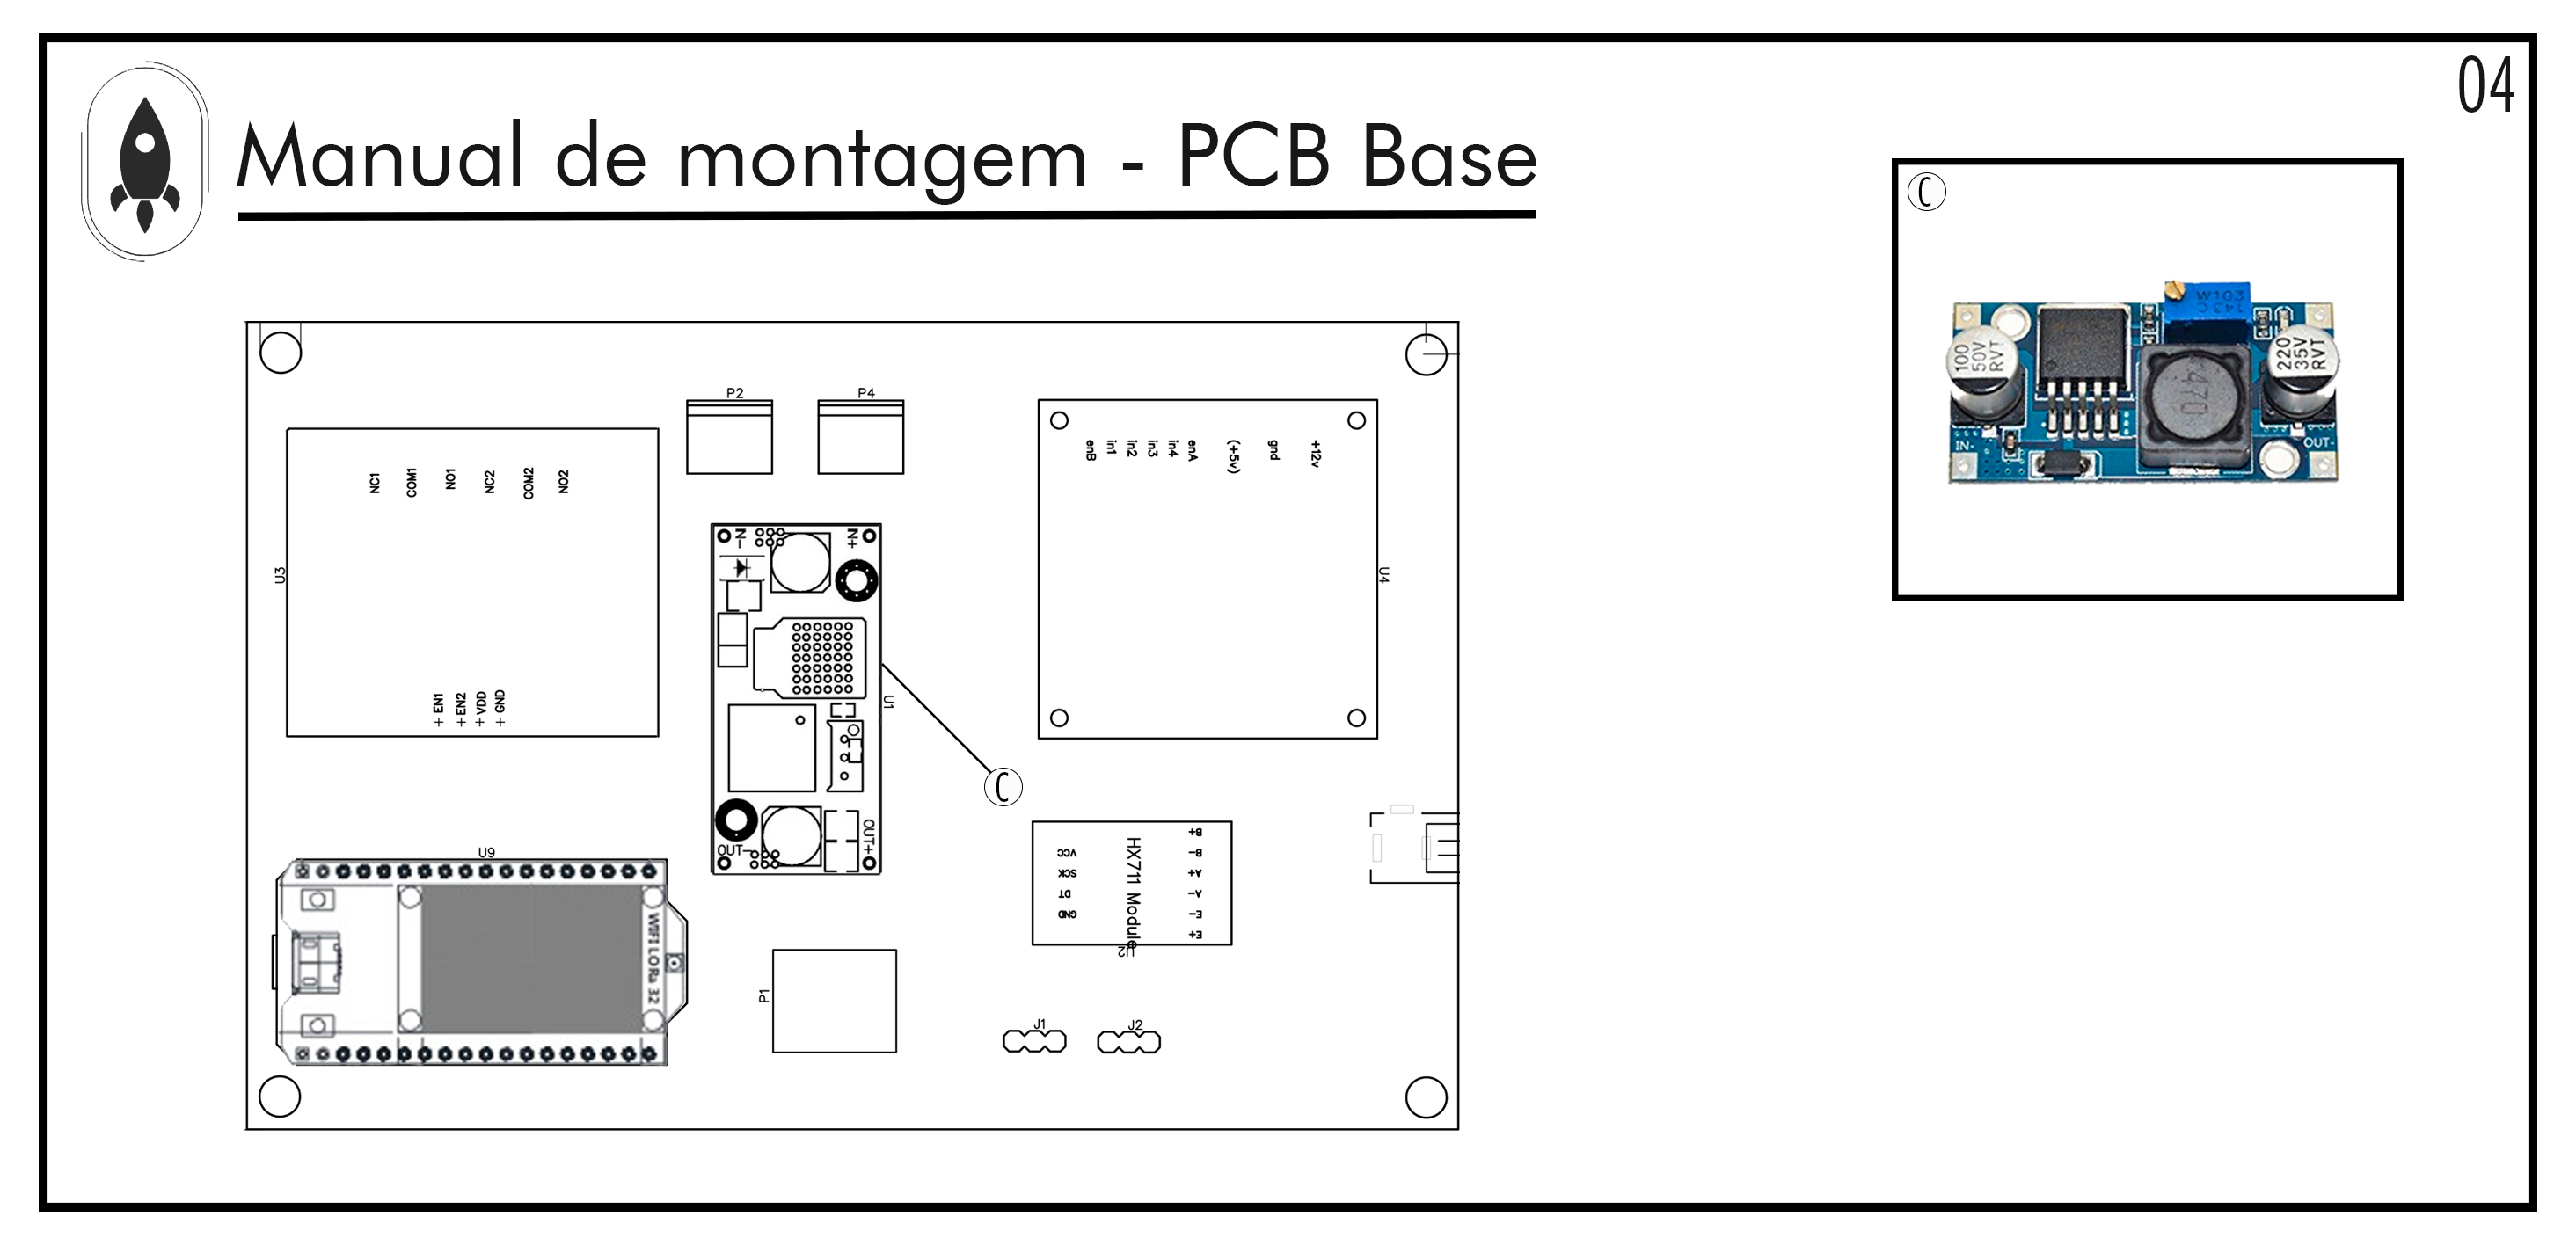
\includegraphics[width=\textwidth]{Figuras/BASE/Pg-04---PL-03.png}
  \caption{LM2596.}
 %{ \footnotesize Fonte: Autores} 
  \label{fig:PCIBASE LM2596}
\end{figure}
\newpage

\par Pegue o componente 'D'(Módulo Conversor Nível Lógico 5V/3.3V -Bidirecional), encaixe-a na posição mostrada \ref{fig:PCIBASE Módulo CONVERSOR LOG  } e solde junto a placa.
\begin{figure}[H]
  \centering
  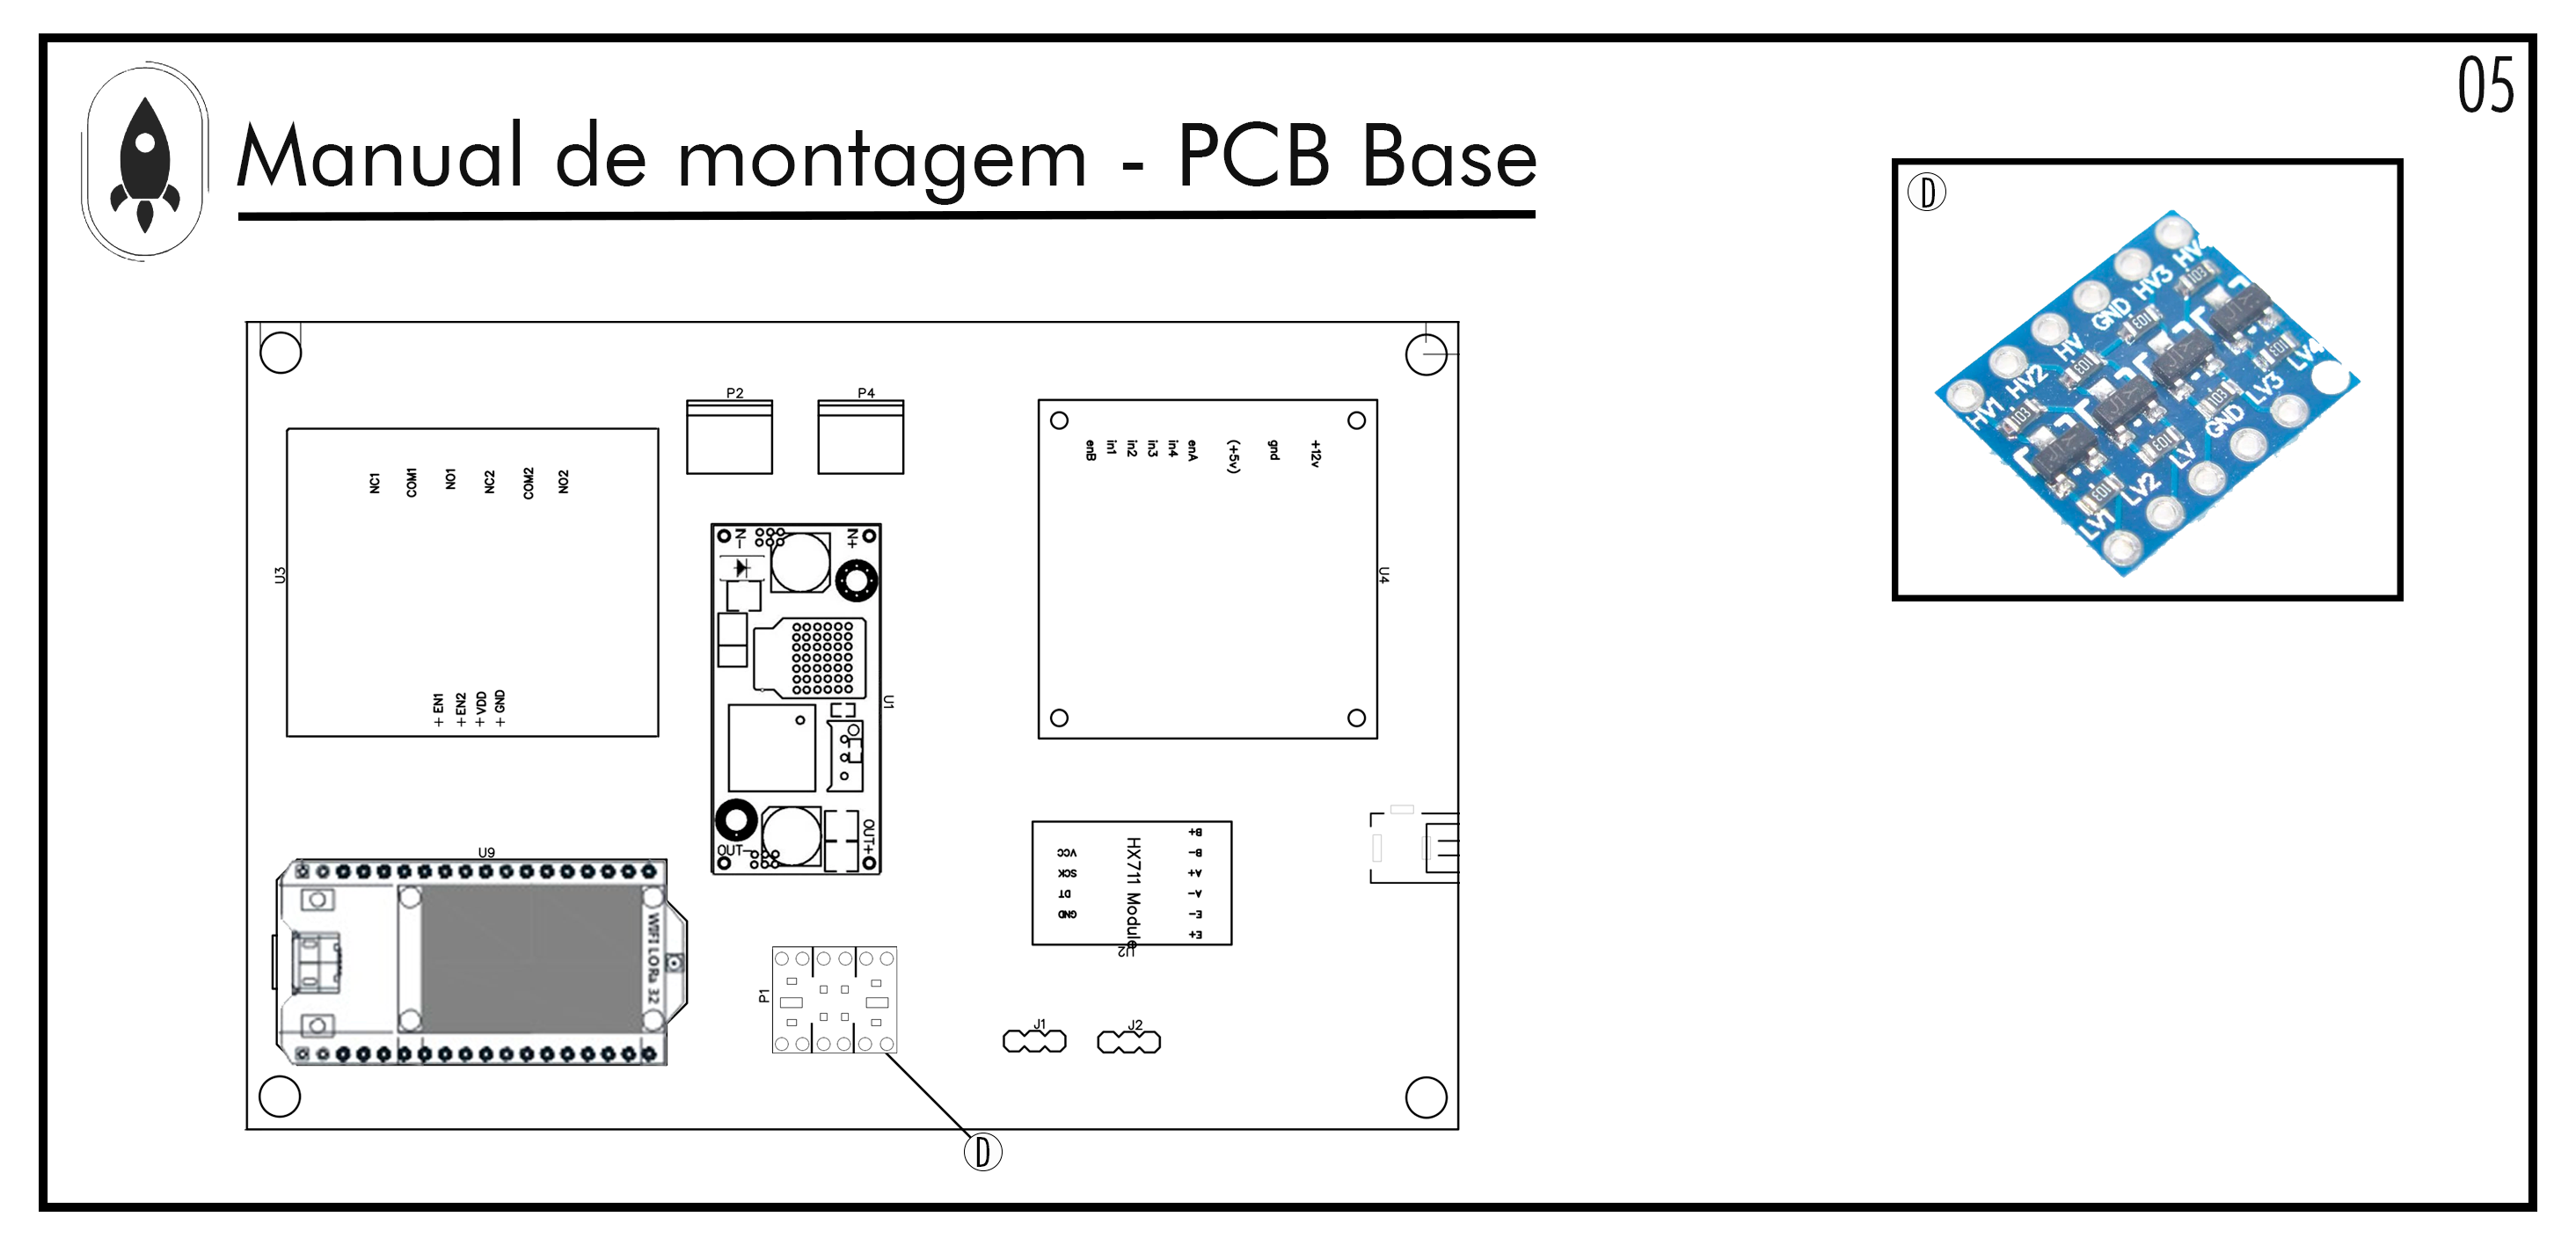
\includegraphics[width=\textwidth]{Figuras/BASE/Pg-05---PL-03.png}
  \caption{Módulo Hx711.}
 %{ \footnotesize Fonte: Autores} 
  \label{fig:PCIBASE Módulo CONVERSOR LOG  }
\end{figure}

\par Pegue o componente 'E'(Módulo Hx711 Célula De Carga Balança 24Bit), encaixe-a na posição mostrada \ref{fig:PCIBASE Módulo Hx711  } e solde junto a placa.
\begin{figure}[H]
  \centering
  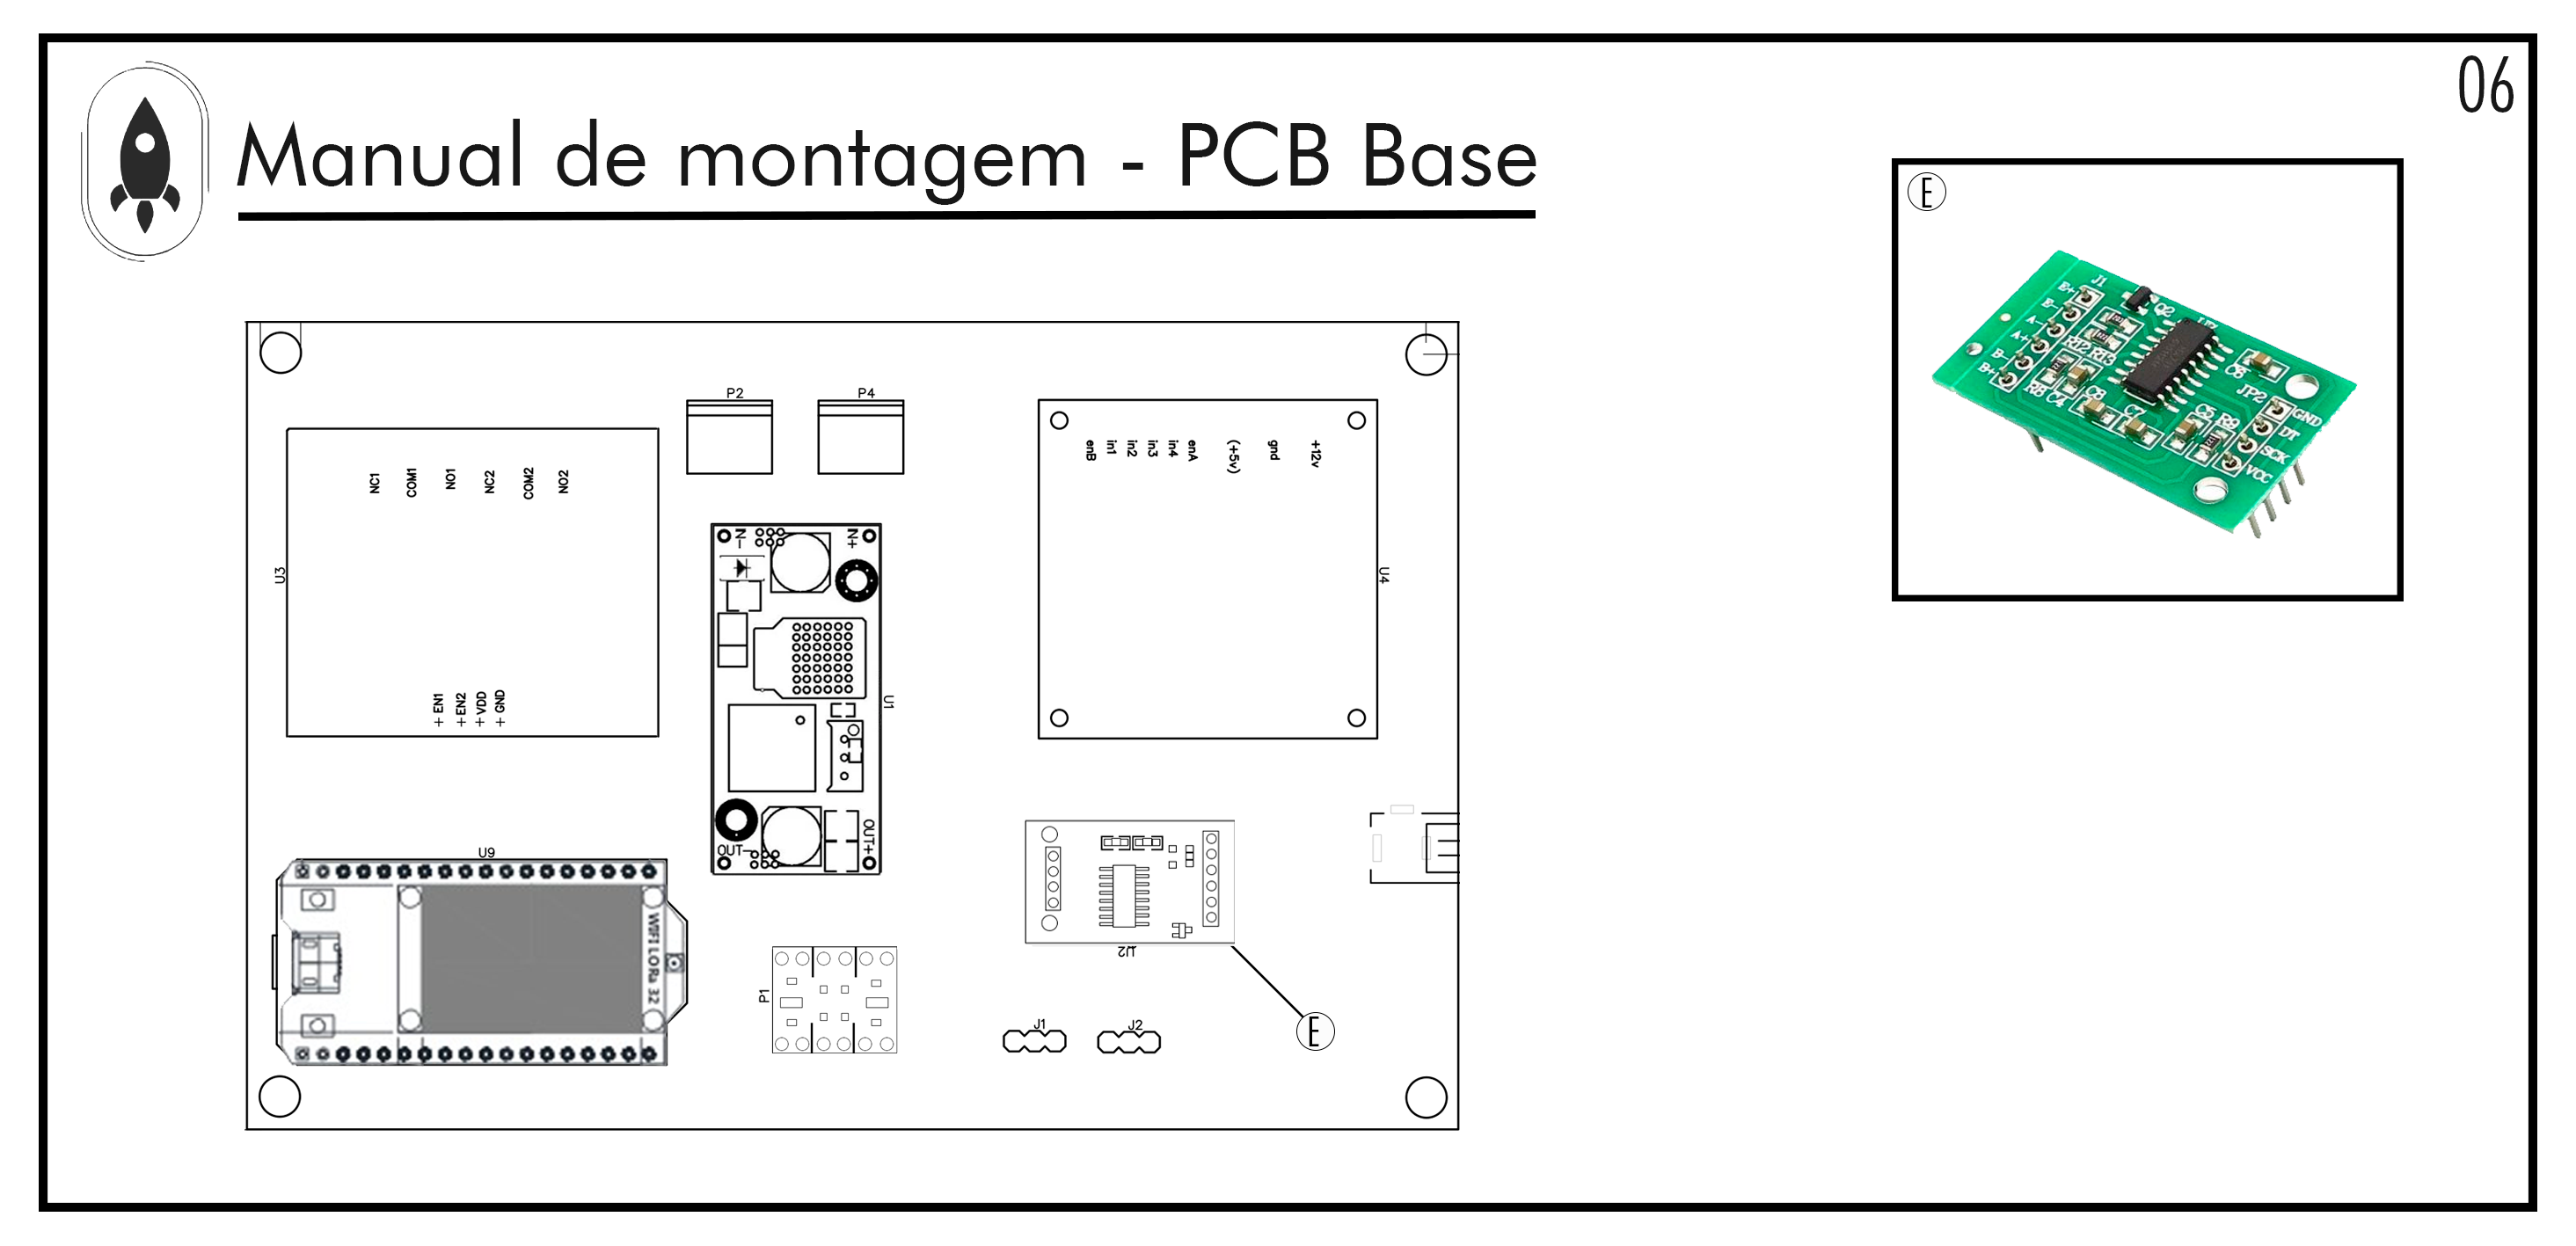
\includegraphics[width=\textwidth]{Figuras/BASE/Pg-06---PL-03.png}
  \caption{Módulo Hx711.}
 %{ \footnotesize Fonte: Autores} 
  \label{fig:PCIBASE Módulo Hx711  }
\end{figure}



\newpage

\par Pegue o componente 'F'(Driver Motor Ponte H L298N), encaixe-a na posição mostrada \ref{fig:PCIBASE ponte H   } e solde junto a placa.
\begin{figure}[H]
  \centering
  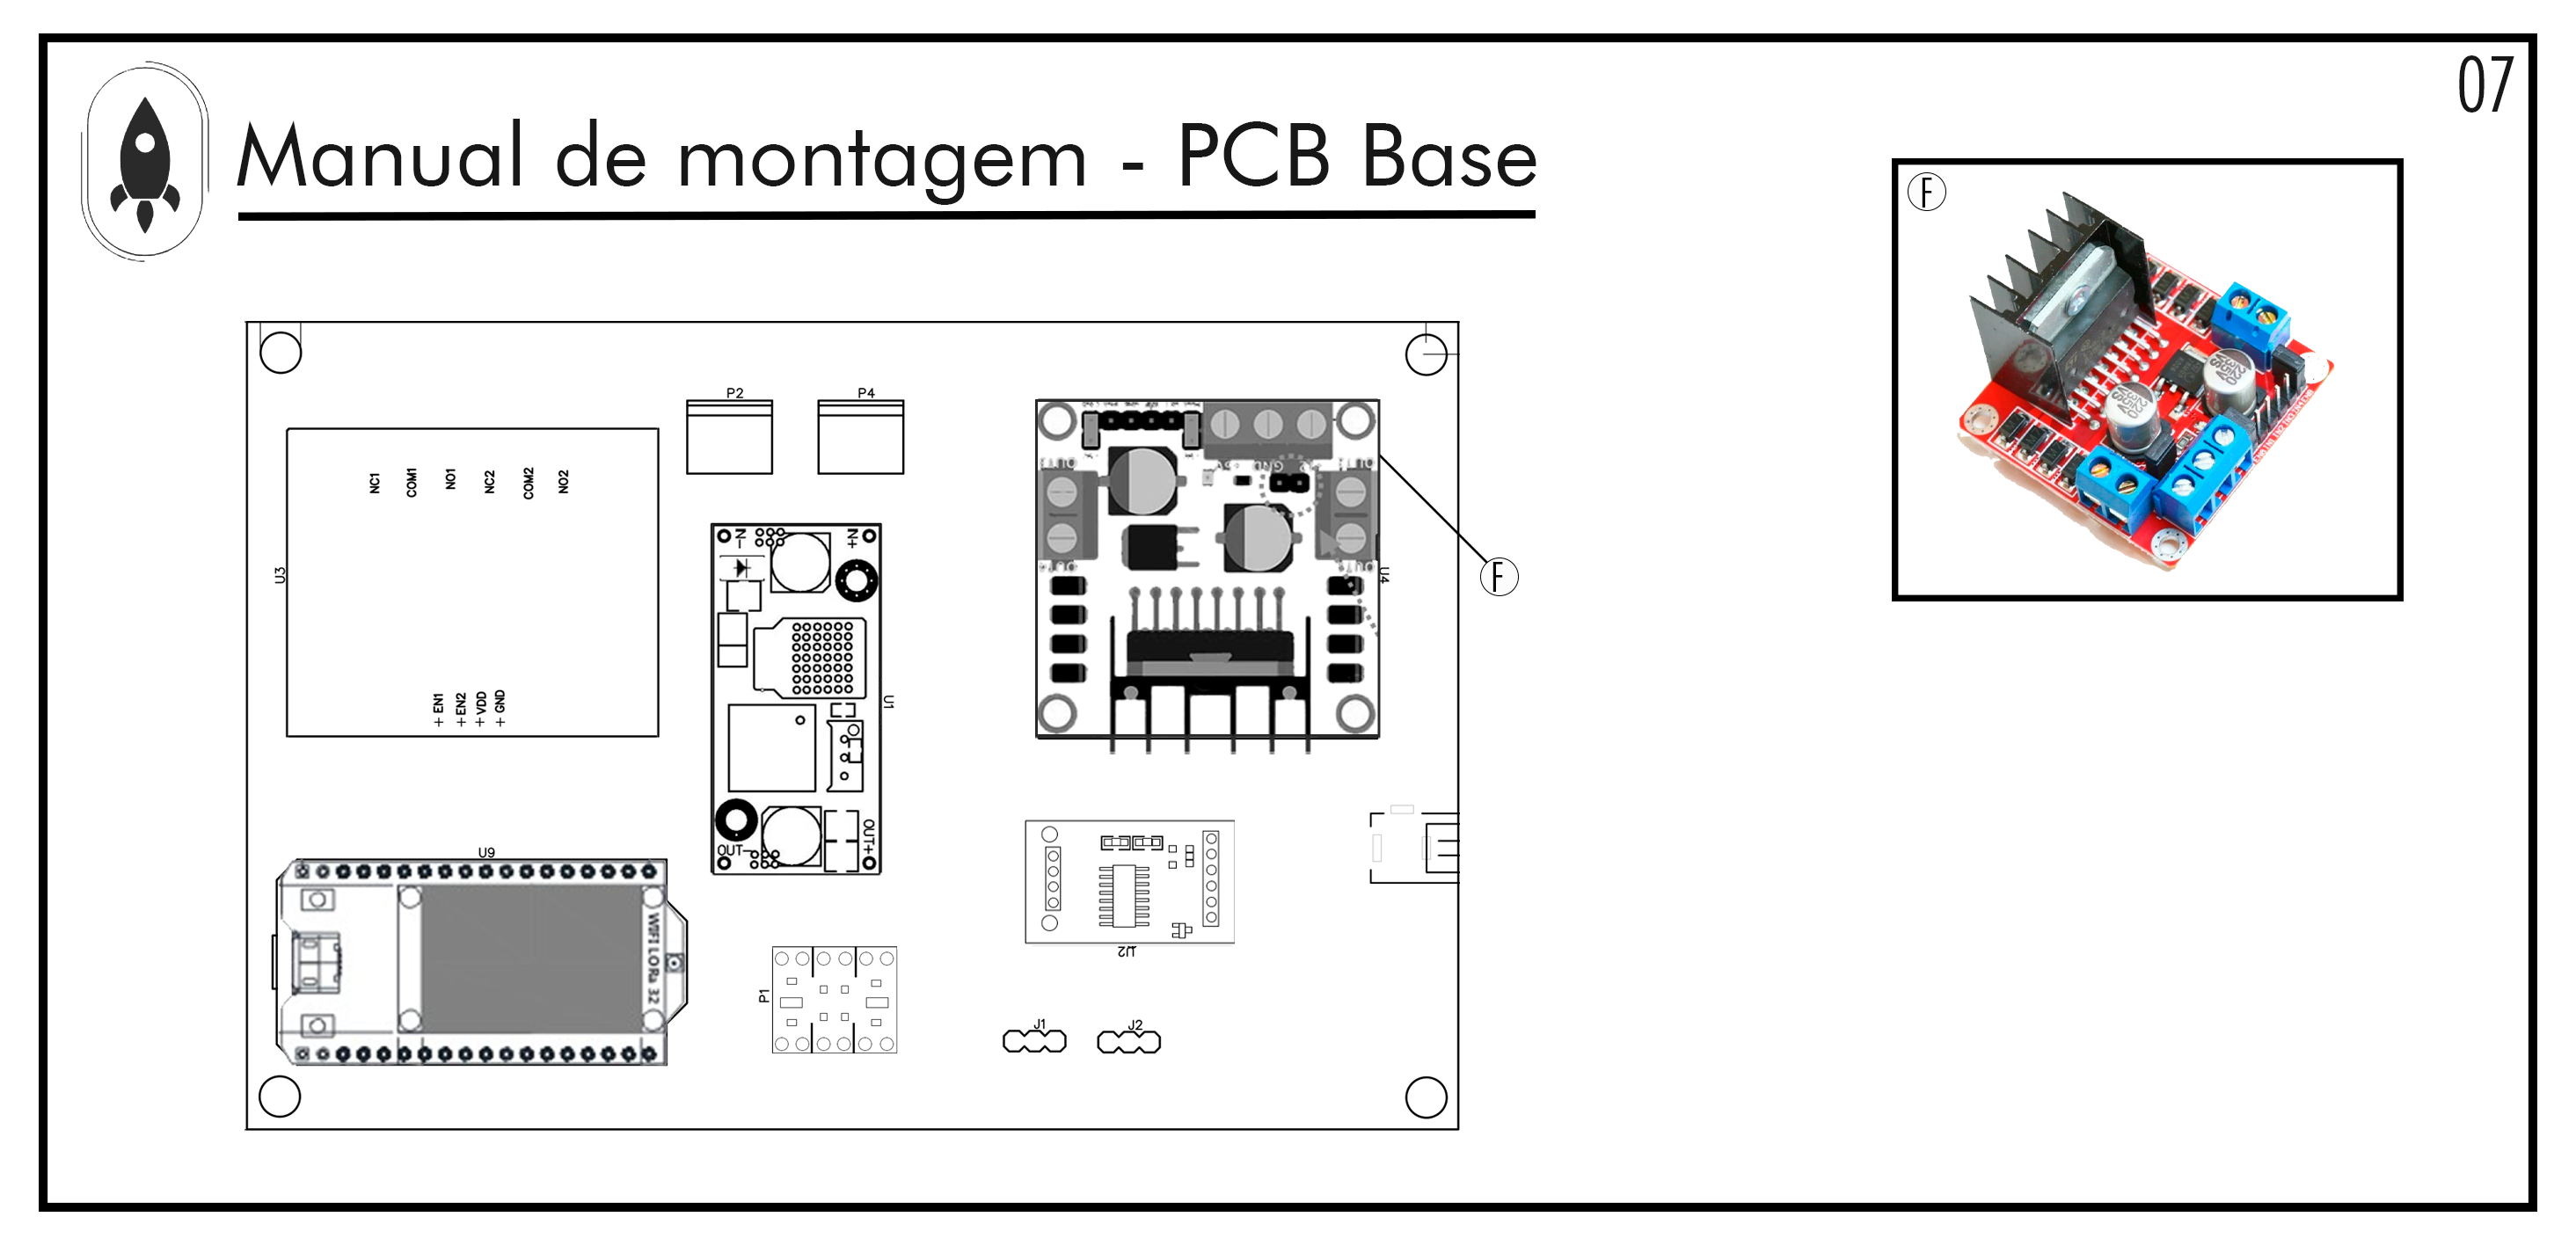
\includegraphics[width=\textwidth]{Figuras/BASE/Pg-07---PL-03.png}
  \caption{Driver Motor Ponte H L298N.}
 %{ \footnotesize Fonte: Autores} 
  \label{fig:PCIBASE ponte H  }
\end{figure}

\par Pegue o componente 'G'( Módulo Relé 5V 2 Canais modelo SRD-05VDC-SL-C), encaixe-a na posição mostrada \ref{fig:PCIBASE Módulo Relé 5V 2 Canais modelo SRD-05VDC-SL-C } e solde junto a placa.
\begin{figure}[H]
  \centering
  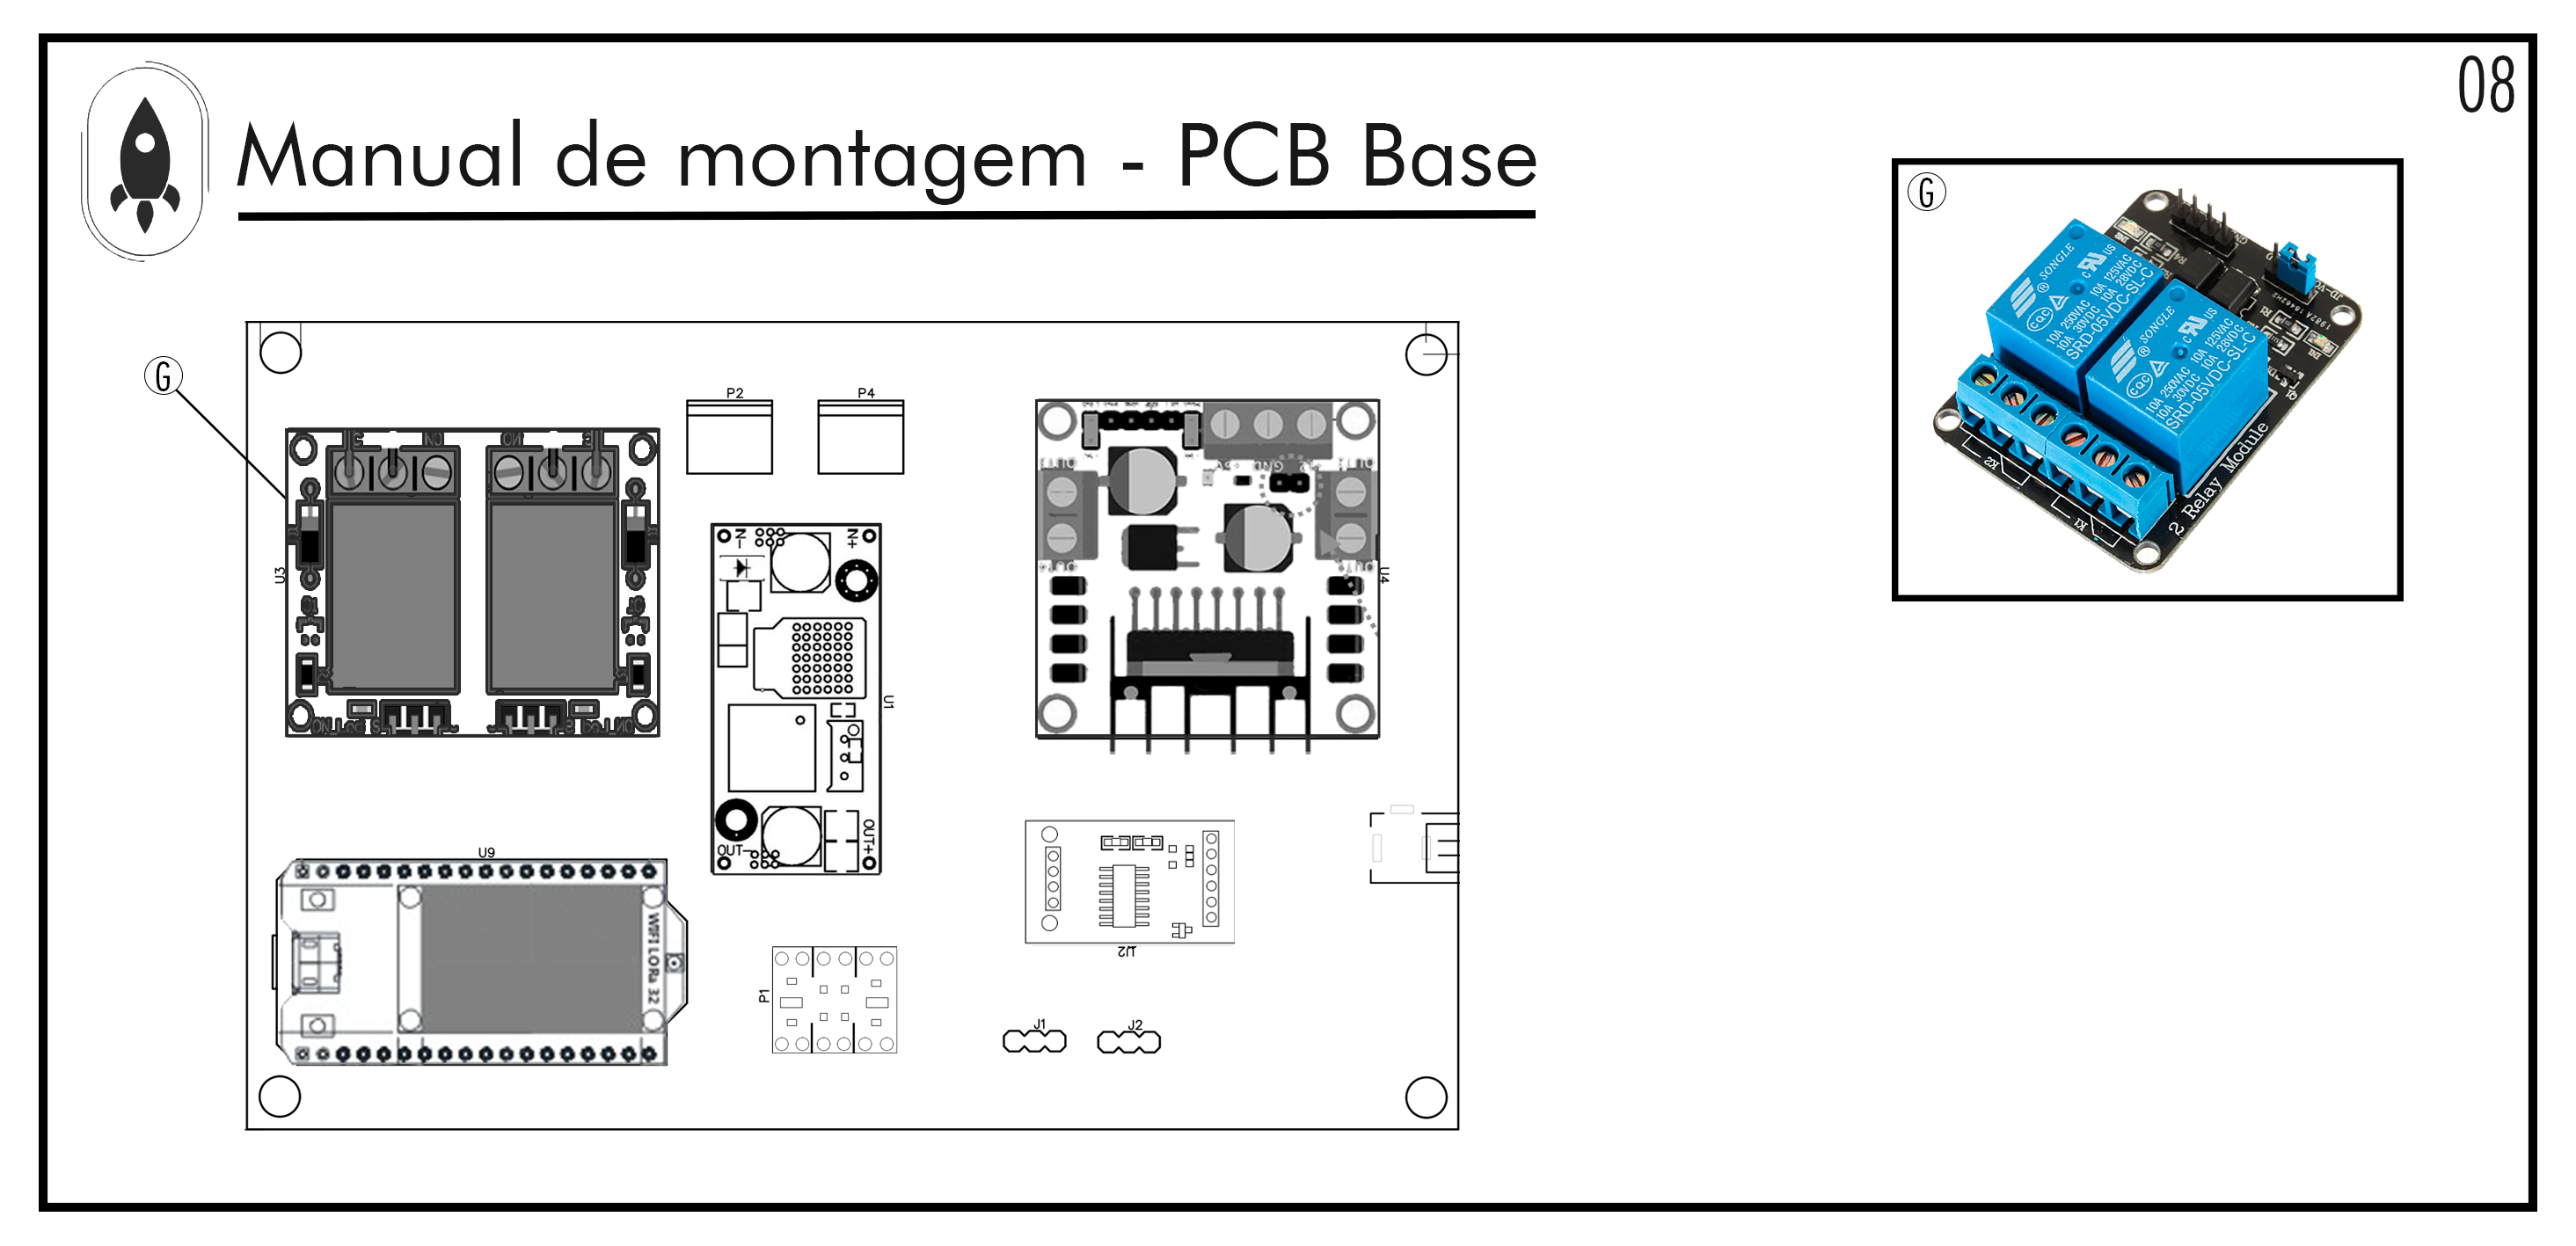
\includegraphics[width=\textwidth]{Figuras/BASE/Pg-08---PL-03.png}
  \caption{ Módulo Relé 5V 2 Canais modelo SRD-05VDC-SL-C.}
 %{ \footnotesize Fonte: Autores} 
  \label{fig:PCIBASE Módulo Relé 5V 2 Canais modelo SRD-05VDC-SL-C }
\end{figure}
\newpage

\par Pegue o componente 'H'(Sensor de Peso 50Kg Célula de Carga ), encaixe-a na posição mostrada \ref{fig:PCIBASE Sensor de Peso 50Kg Célula de Carga  }   e solde junto a placa.
\begin{figure}[H]
  \centering
  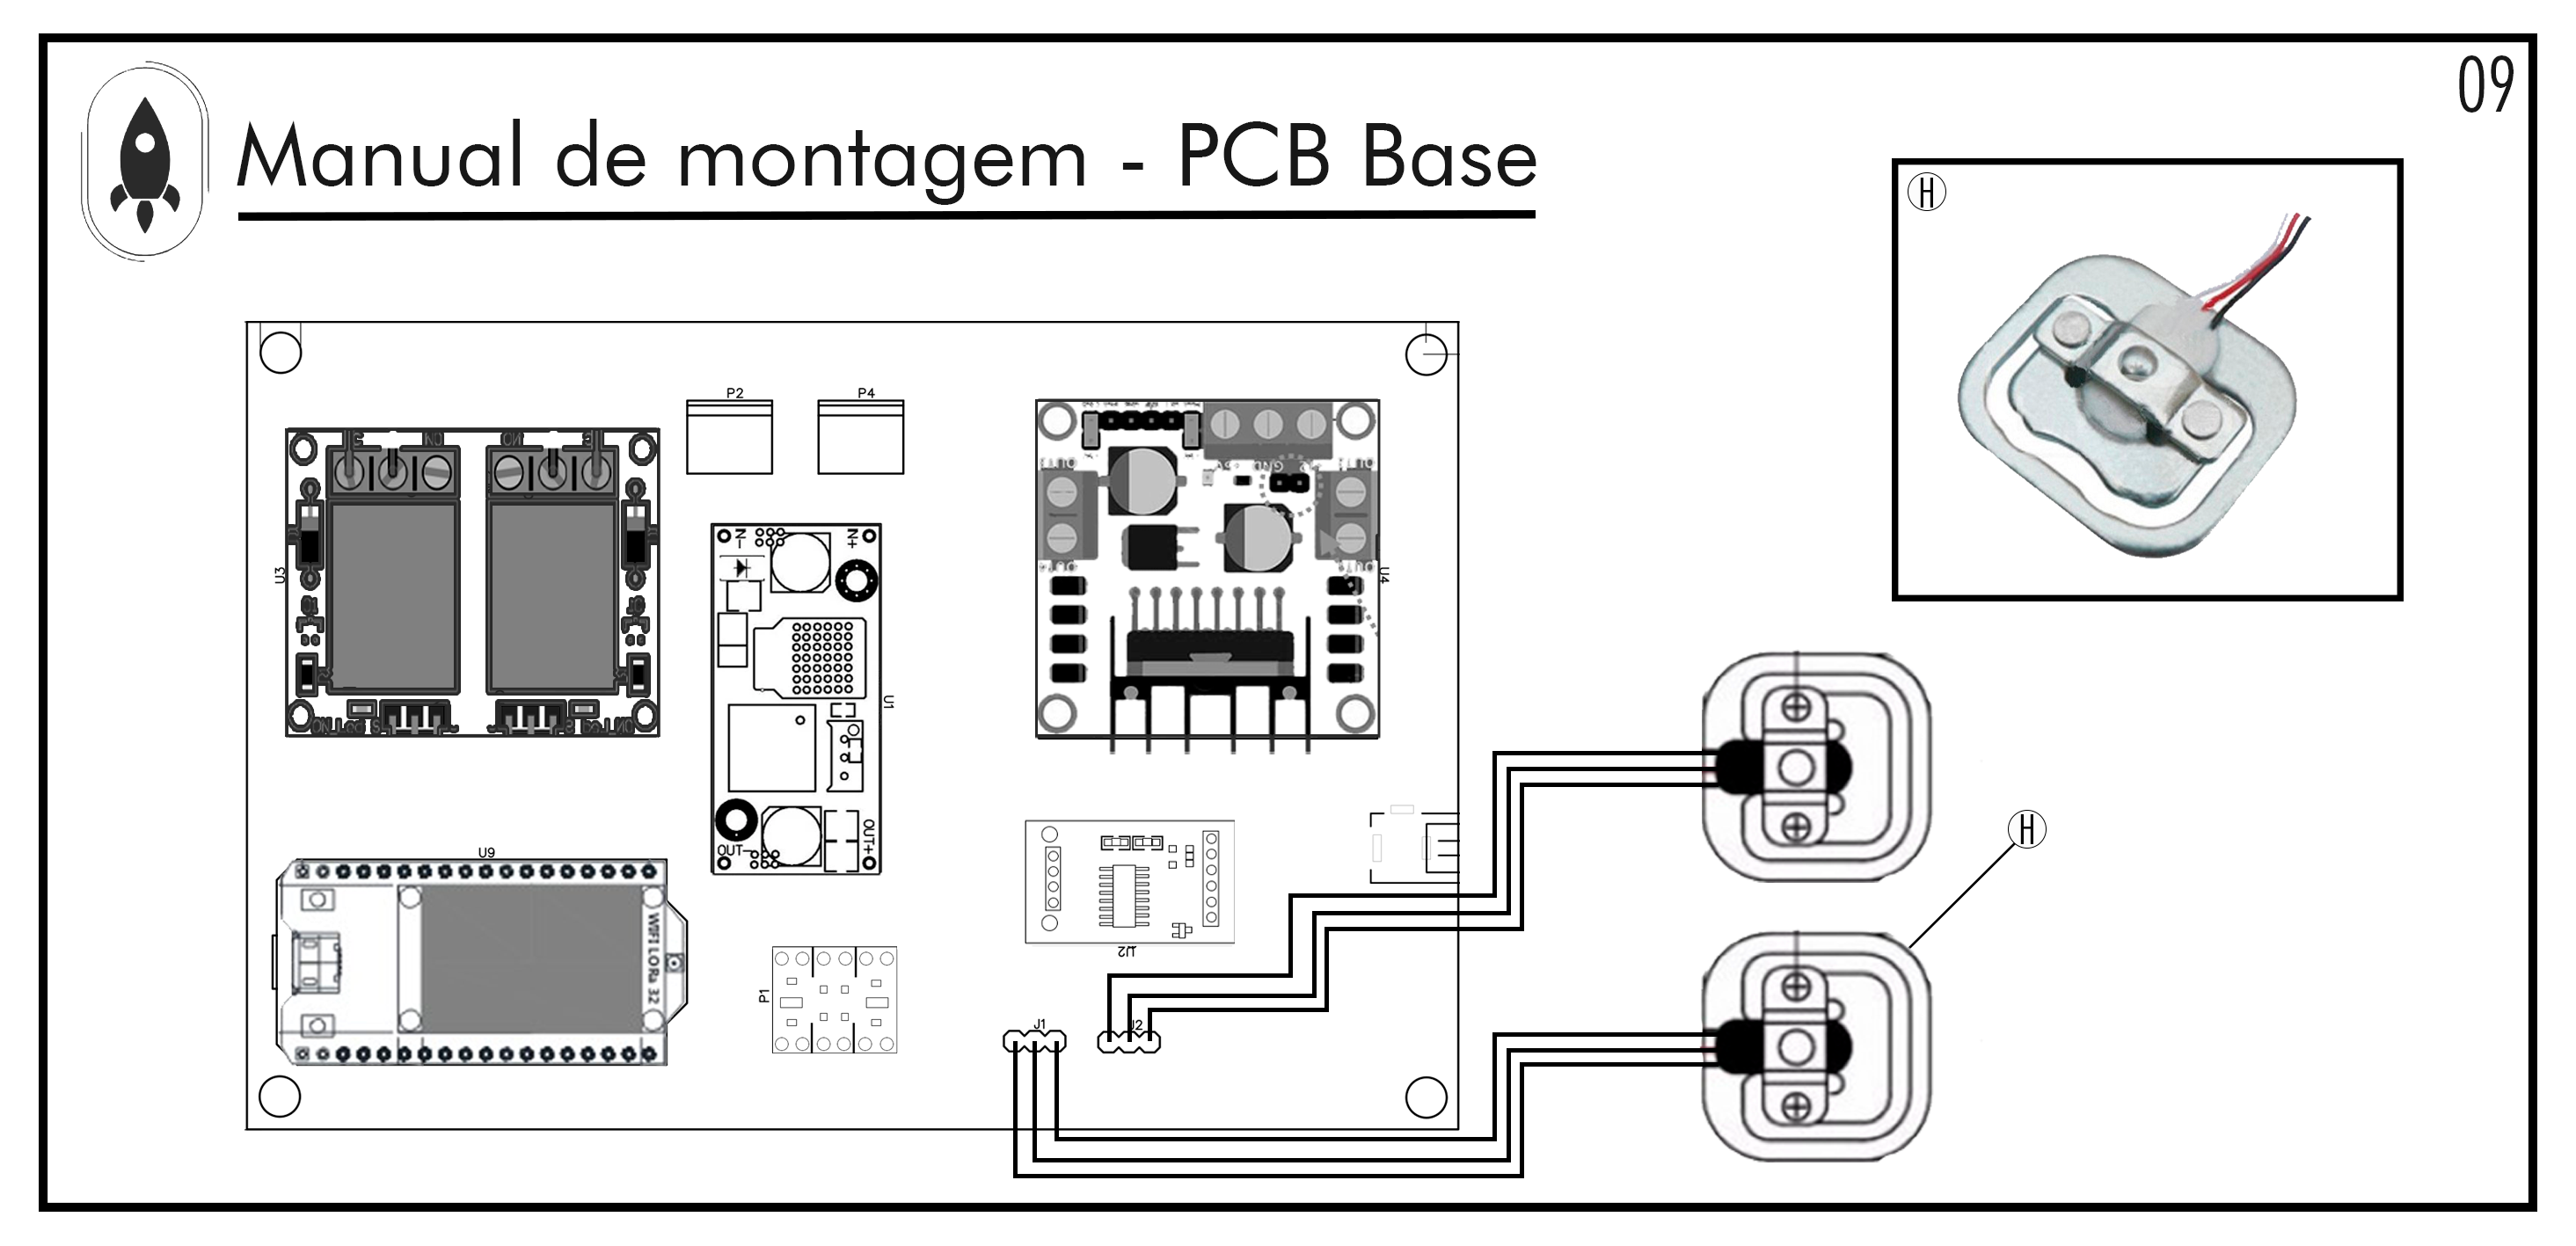
\includegraphics[width=\textwidth]{Figuras/BASE/Pg-09---PL-03.png}
  \caption{Sensor de Peso 50Kg Célula de Carga.}
 %{ \footnotesize Fonte: Autores} 
  \label{fig:PCIBASE Sensor de Peso 50Kg Célula de Carga  }
\end{figure}

\par Pegue o componente 'I'(Conector fêmea Jack P4 2,5mm), encaixe-a na posição mostrada \ref{fig:PCIBASE  Conector Jack P4 2,5mm    }   e solde junto a placa.
\begin{figure}[H]
  \centering
  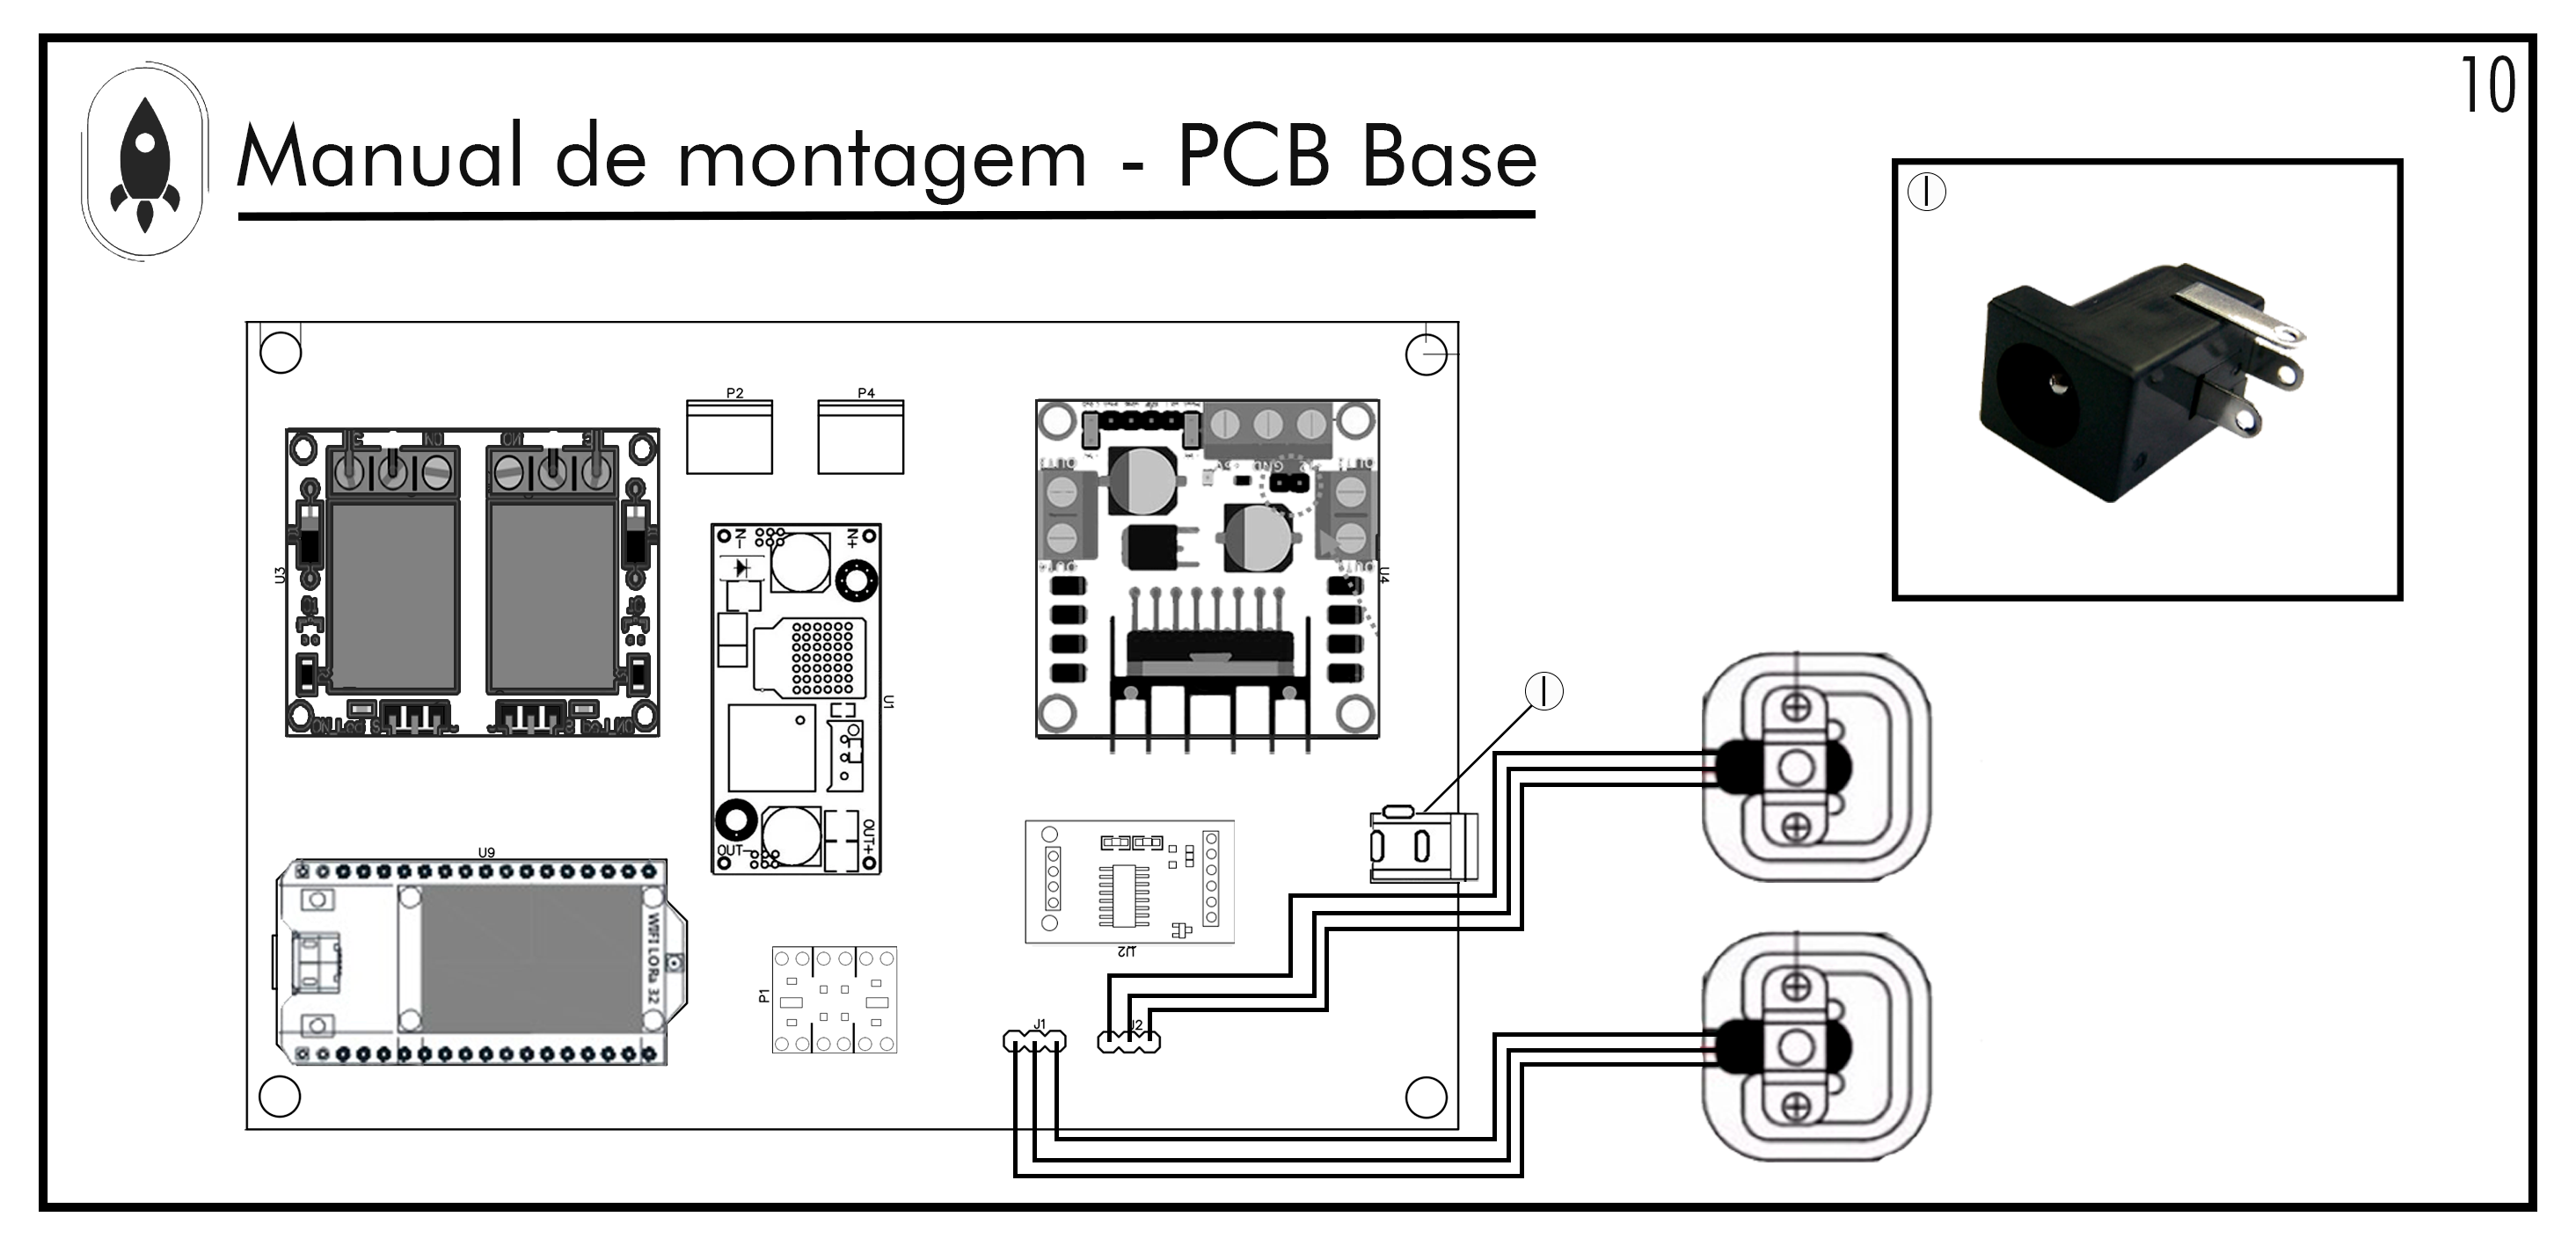
\includegraphics[width=\textwidth]{Figuras/BASE/Pg-10---PL-03.png}
  \caption{ Conector fêmea Jack P4 2,5mm.}
 %{ \footnotesize Fonte: Autores} 
  \label{fig:PCIBASE  Conector Jack P4 2,5mm  }
\end{figure}

\newpage
\par Pegue o componente 'J'(Borne Conector Kre 2 Vias), encaixe-a na posição mostrada \ref{fig:PCIBASE Borne Conector Kre 2 Vias }   e solde junto a placa.
\begin{figure}[H]
  \centering
  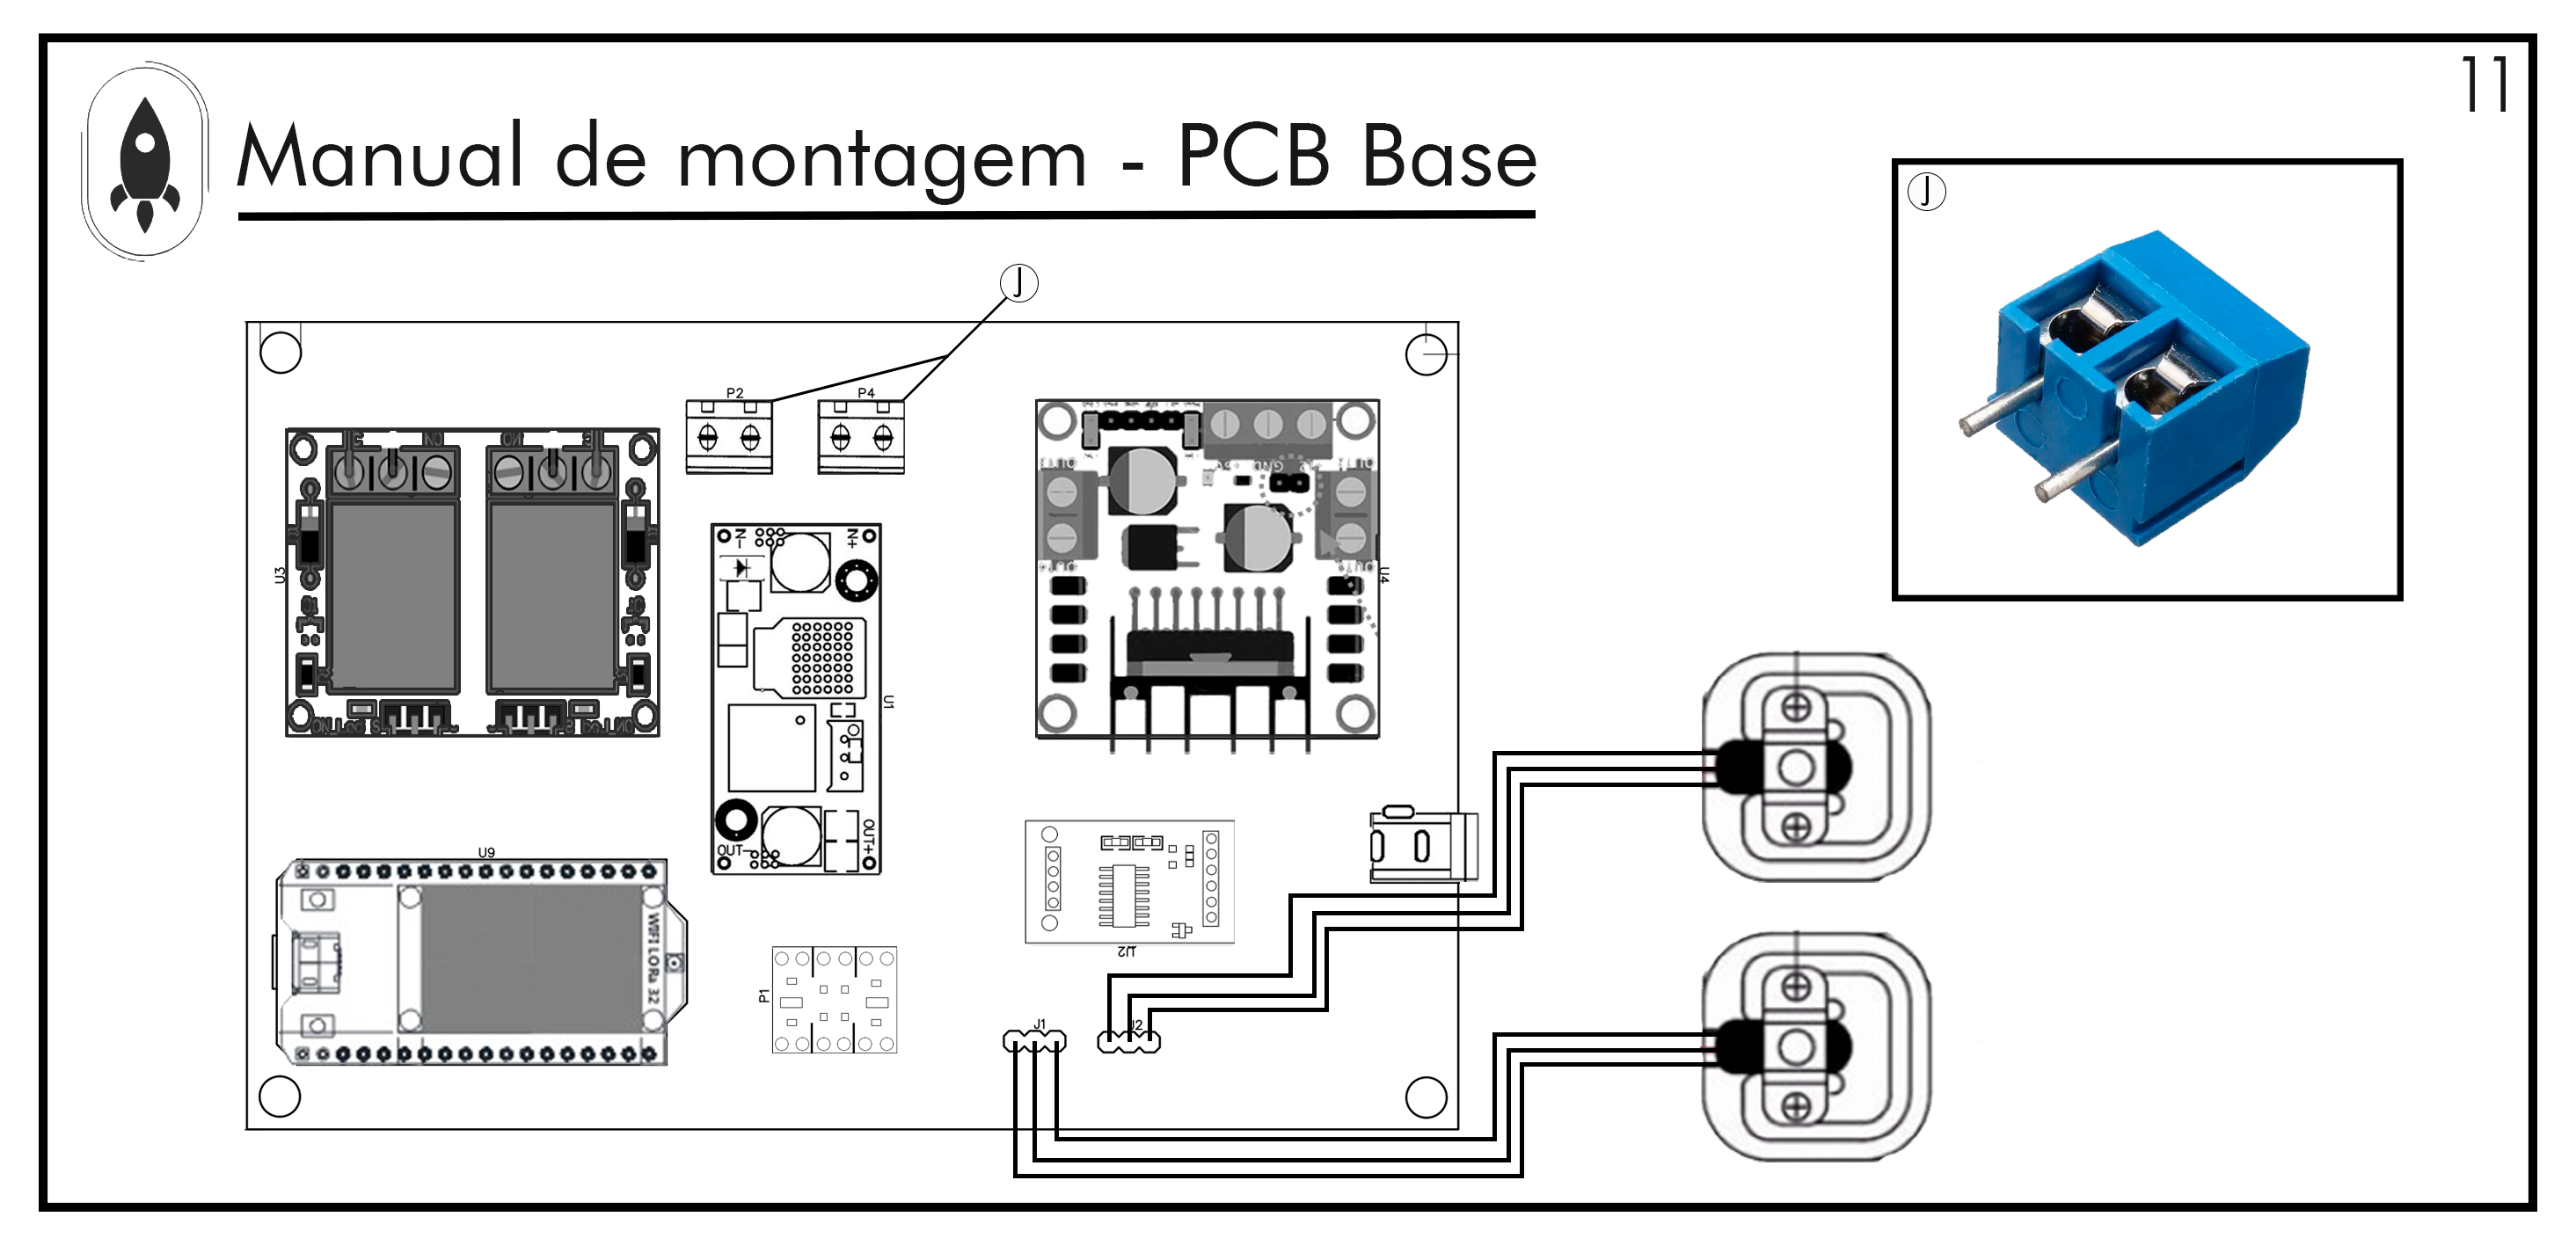
\includegraphics[width=\textwidth]{Figuras/BASE/Pg-11---PL-03.png}
  \caption{Borne Conector Kre 2 Vias.}
 %{ \footnotesize Fonte: Autores} 
  \label{fig:PCIBASE Borne Conector Kre 2 Vias  }
\end{figure}

\par Para a fixação da placa em seu recipiente utilize os parafusos e a porca extensora, componentes 'K' e 'L' e siga as instruções da seção \ref{sec:fixação }.

\subsection{Placas de Circuito Impresso-Foguete}

\subsubsection{Lista de Materiais}

\par Primeiramente é necessário ter em mão todos os componentes para sua montagem \ref{fig:Lista de materiais foguete}.

\begin{table}[H]
\centering
\begin{tabular}{|m{1.9cm} |m{1.8cm} |m{7.3cm}|m{4cm}|}
\hline
\begin{center}Identificador\end{center} &\begin{center} Quantidade\end{center} & \begin{center}Componente\end{center} &\begin{center} Part Number\end{center} \\\hline
A&01 &  PCI- Foguete  & -  \\\hline
B &01&Lora Esp32 Sx1278 Com Display  Oled Wifi bluetooth 915mhz& Sx1278 \\\hline
 
C&01 &  Conversor DC-DC Step Down-LM2596 (12~5V)
& LM2596 \\\hline

D&01 & Conector Jack J4 DC Fêmea &  Jack Fêmea  \\\hline

E&01&Sensor De Pressão e Temperatura BMP 280 & BST-BMP280-DS001-11 \\\hline

F&01 &  Módulo Relé 5V 2 Canais &   SRD-05VDC-SL-C \\\hline

G &01 & Módulo Gps  Gy-gps6m v2 & GPS NEO6M \\\hline

H&01 & Módulo Cartão de Memória MICRO SD CARD & B01IPCAP72 \\\hline

I&01&Conector Borne KRE 2 Vias & KRE Kf301 \\\hline

J&05&Parafuso Máquina Cabeça Chata Phillips M5 X 20mm &  Phillips M5 X 20mm \\\hline

K&05& porca de bronze espaçador hexagonal M5 X 12mm & -  \\\hline

\end{tabular}
\caption{Lista de componentes}
\end{table}


\subsubsection{Instruções}


\begin{figure}[H]
  \centering
  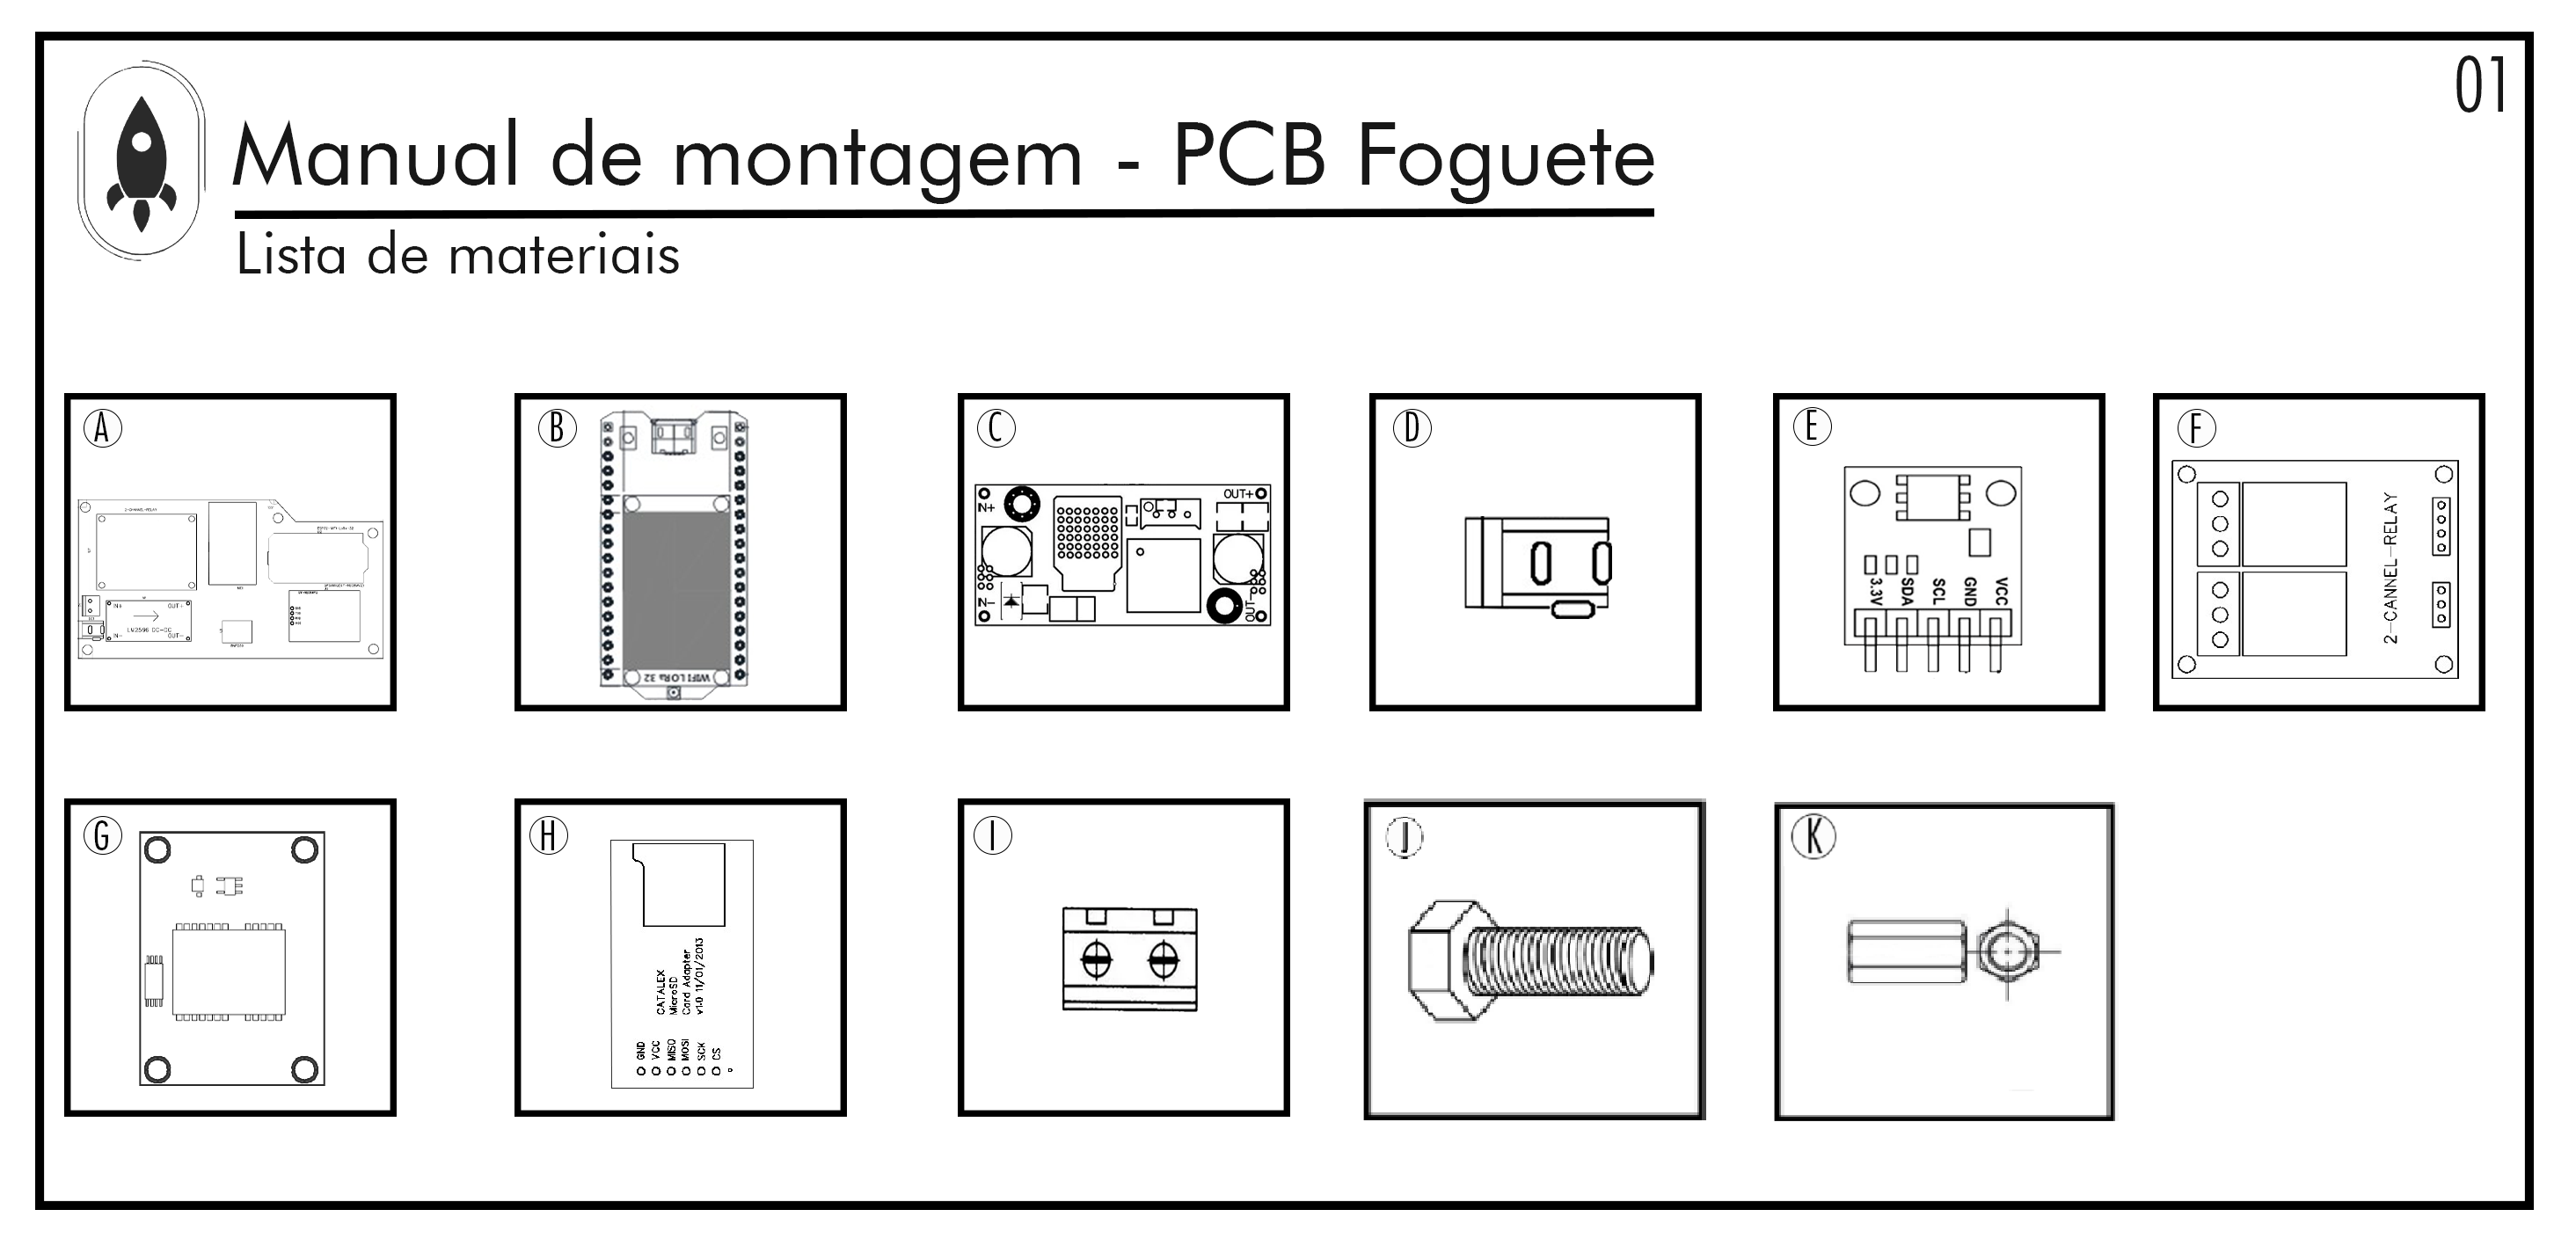
\includegraphics[width=\textwidth]{Figuras/FOGUETE/Pg-01---PL-02.png}
  \caption{Lista de Materiais.} 
 %{ \footnotesize Fonte: Autores} 
  \label{fig:Lista de materiais foguete}
\end{figure}



\par Com todos os componentes em mãos, pegue componente 'A'(PCI-Foguete) prepare-a para soldagem dos componentes passando uma fina camada de solda nos pads da PCI.

\begin{figure}[H]
  \centering
  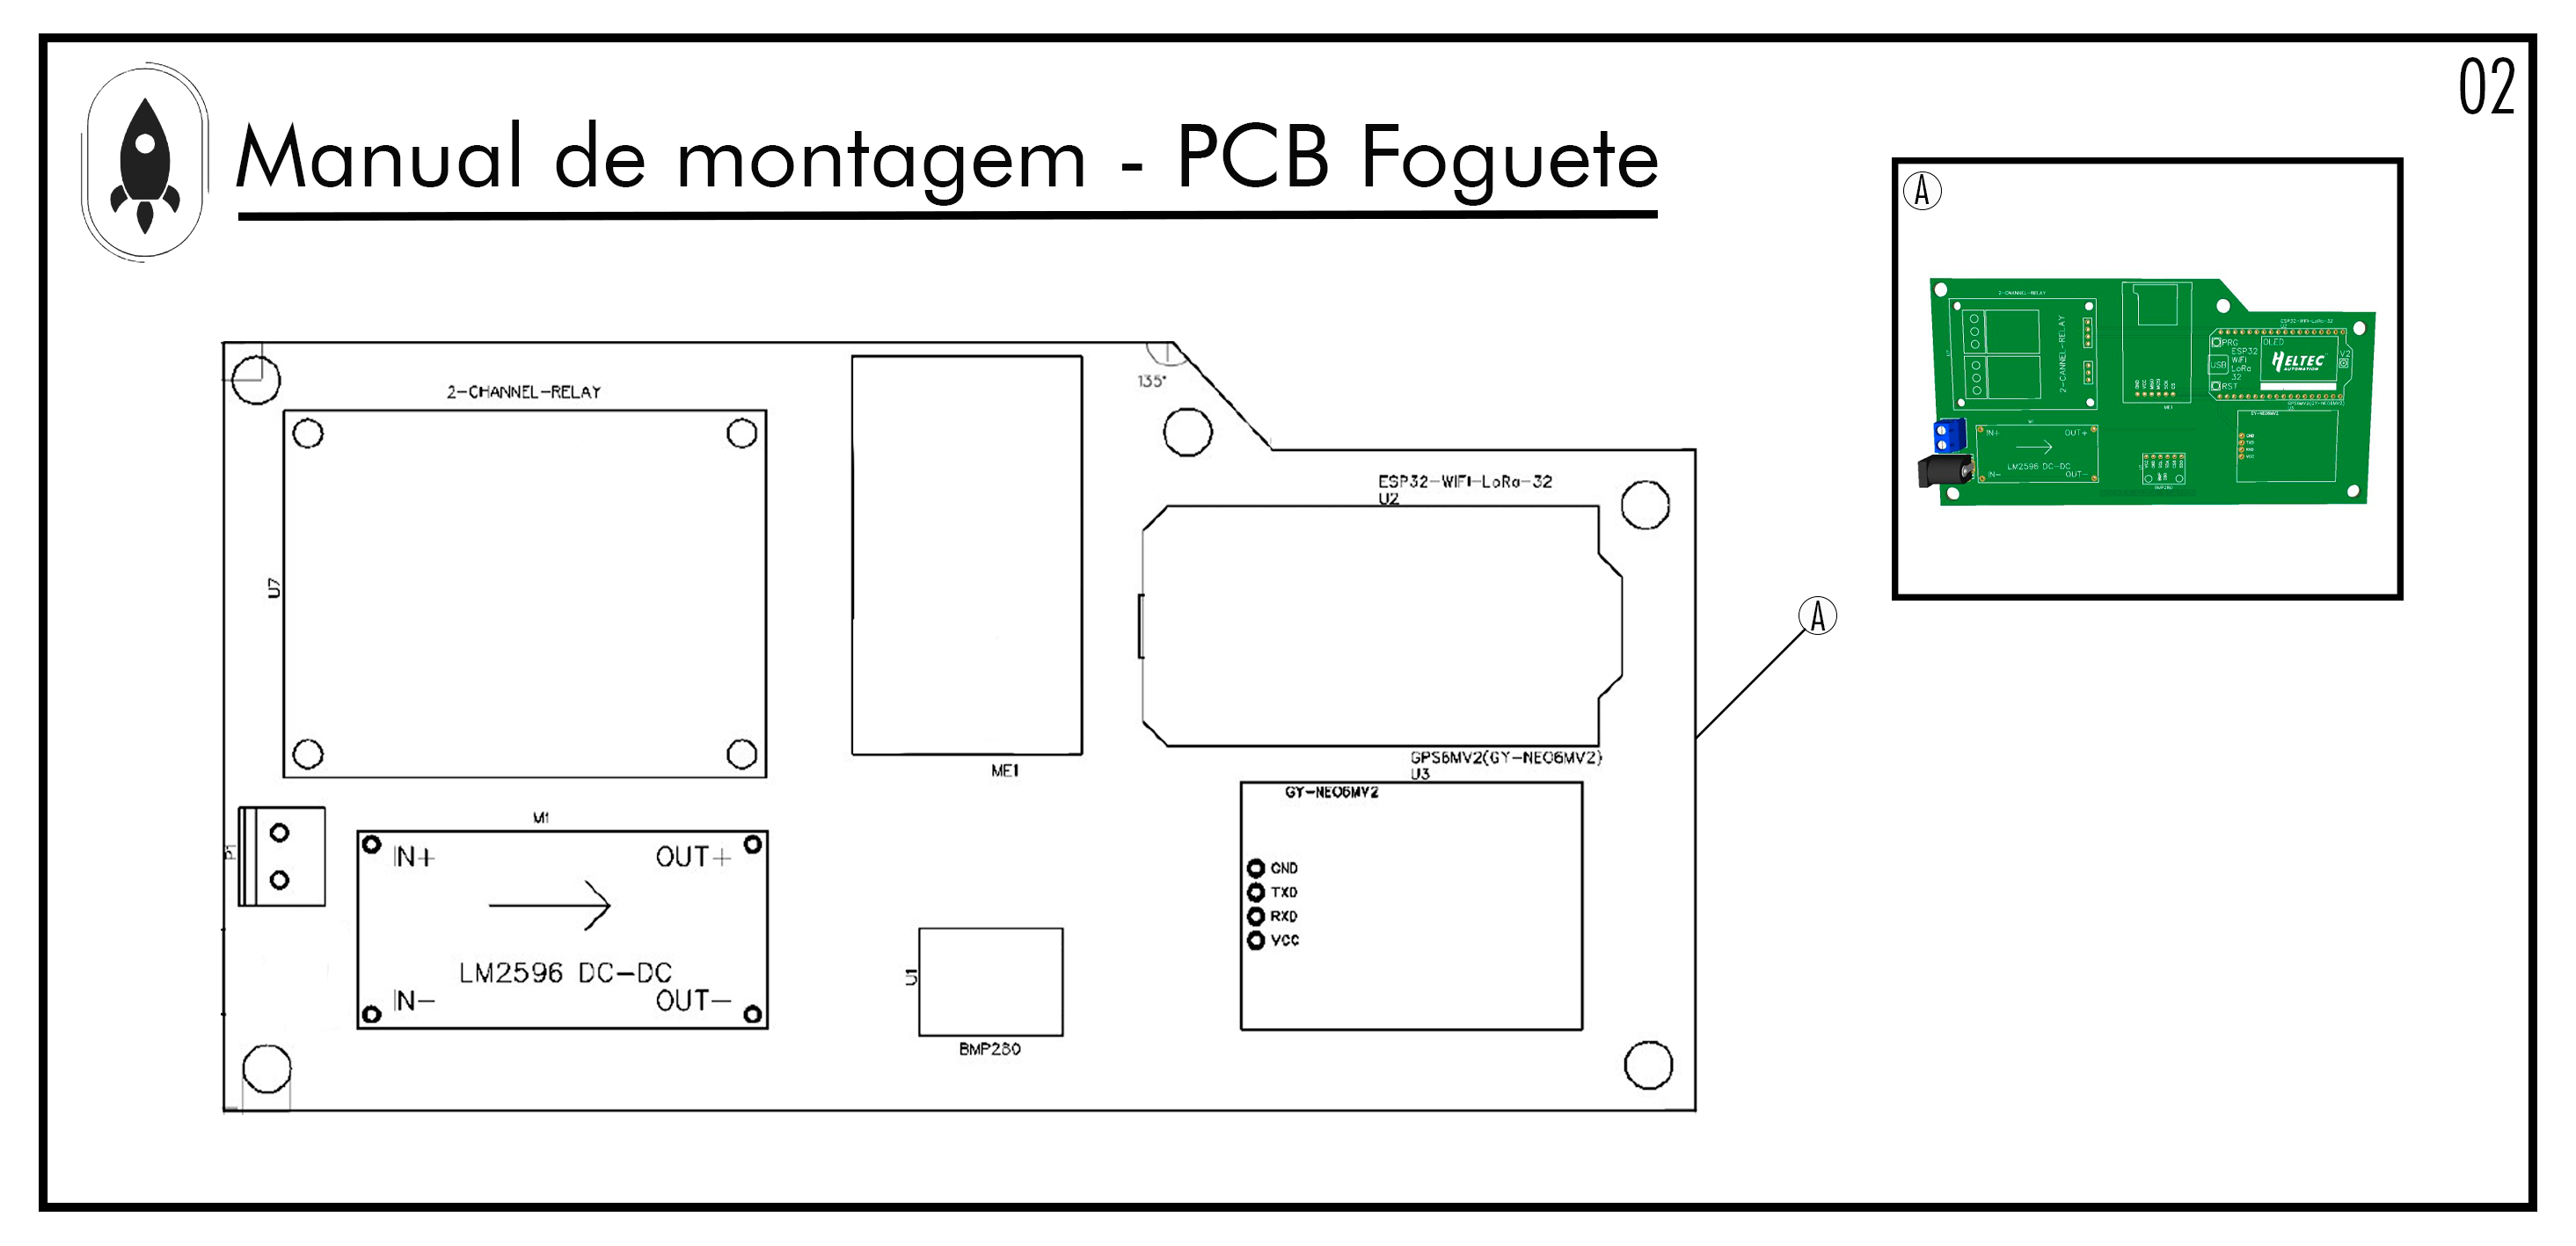
\includegraphics[width=\textwidth]{Figuras/FOGUETE/Pg-02---PL-02.png}
  \caption{PCI do foguete.}
 %{ \footnotesize Fonte: Autores} 
  \label{fig:PCIFoguete}
\end{figure}

\par Pegue o componente 'B'(ESP32 LoRa WiFi), encaixe-a na posição mostrada \ref{fig:PCIFoguete LORA} e solde junto a placa.
\begin{figure}[H]
  \centering
  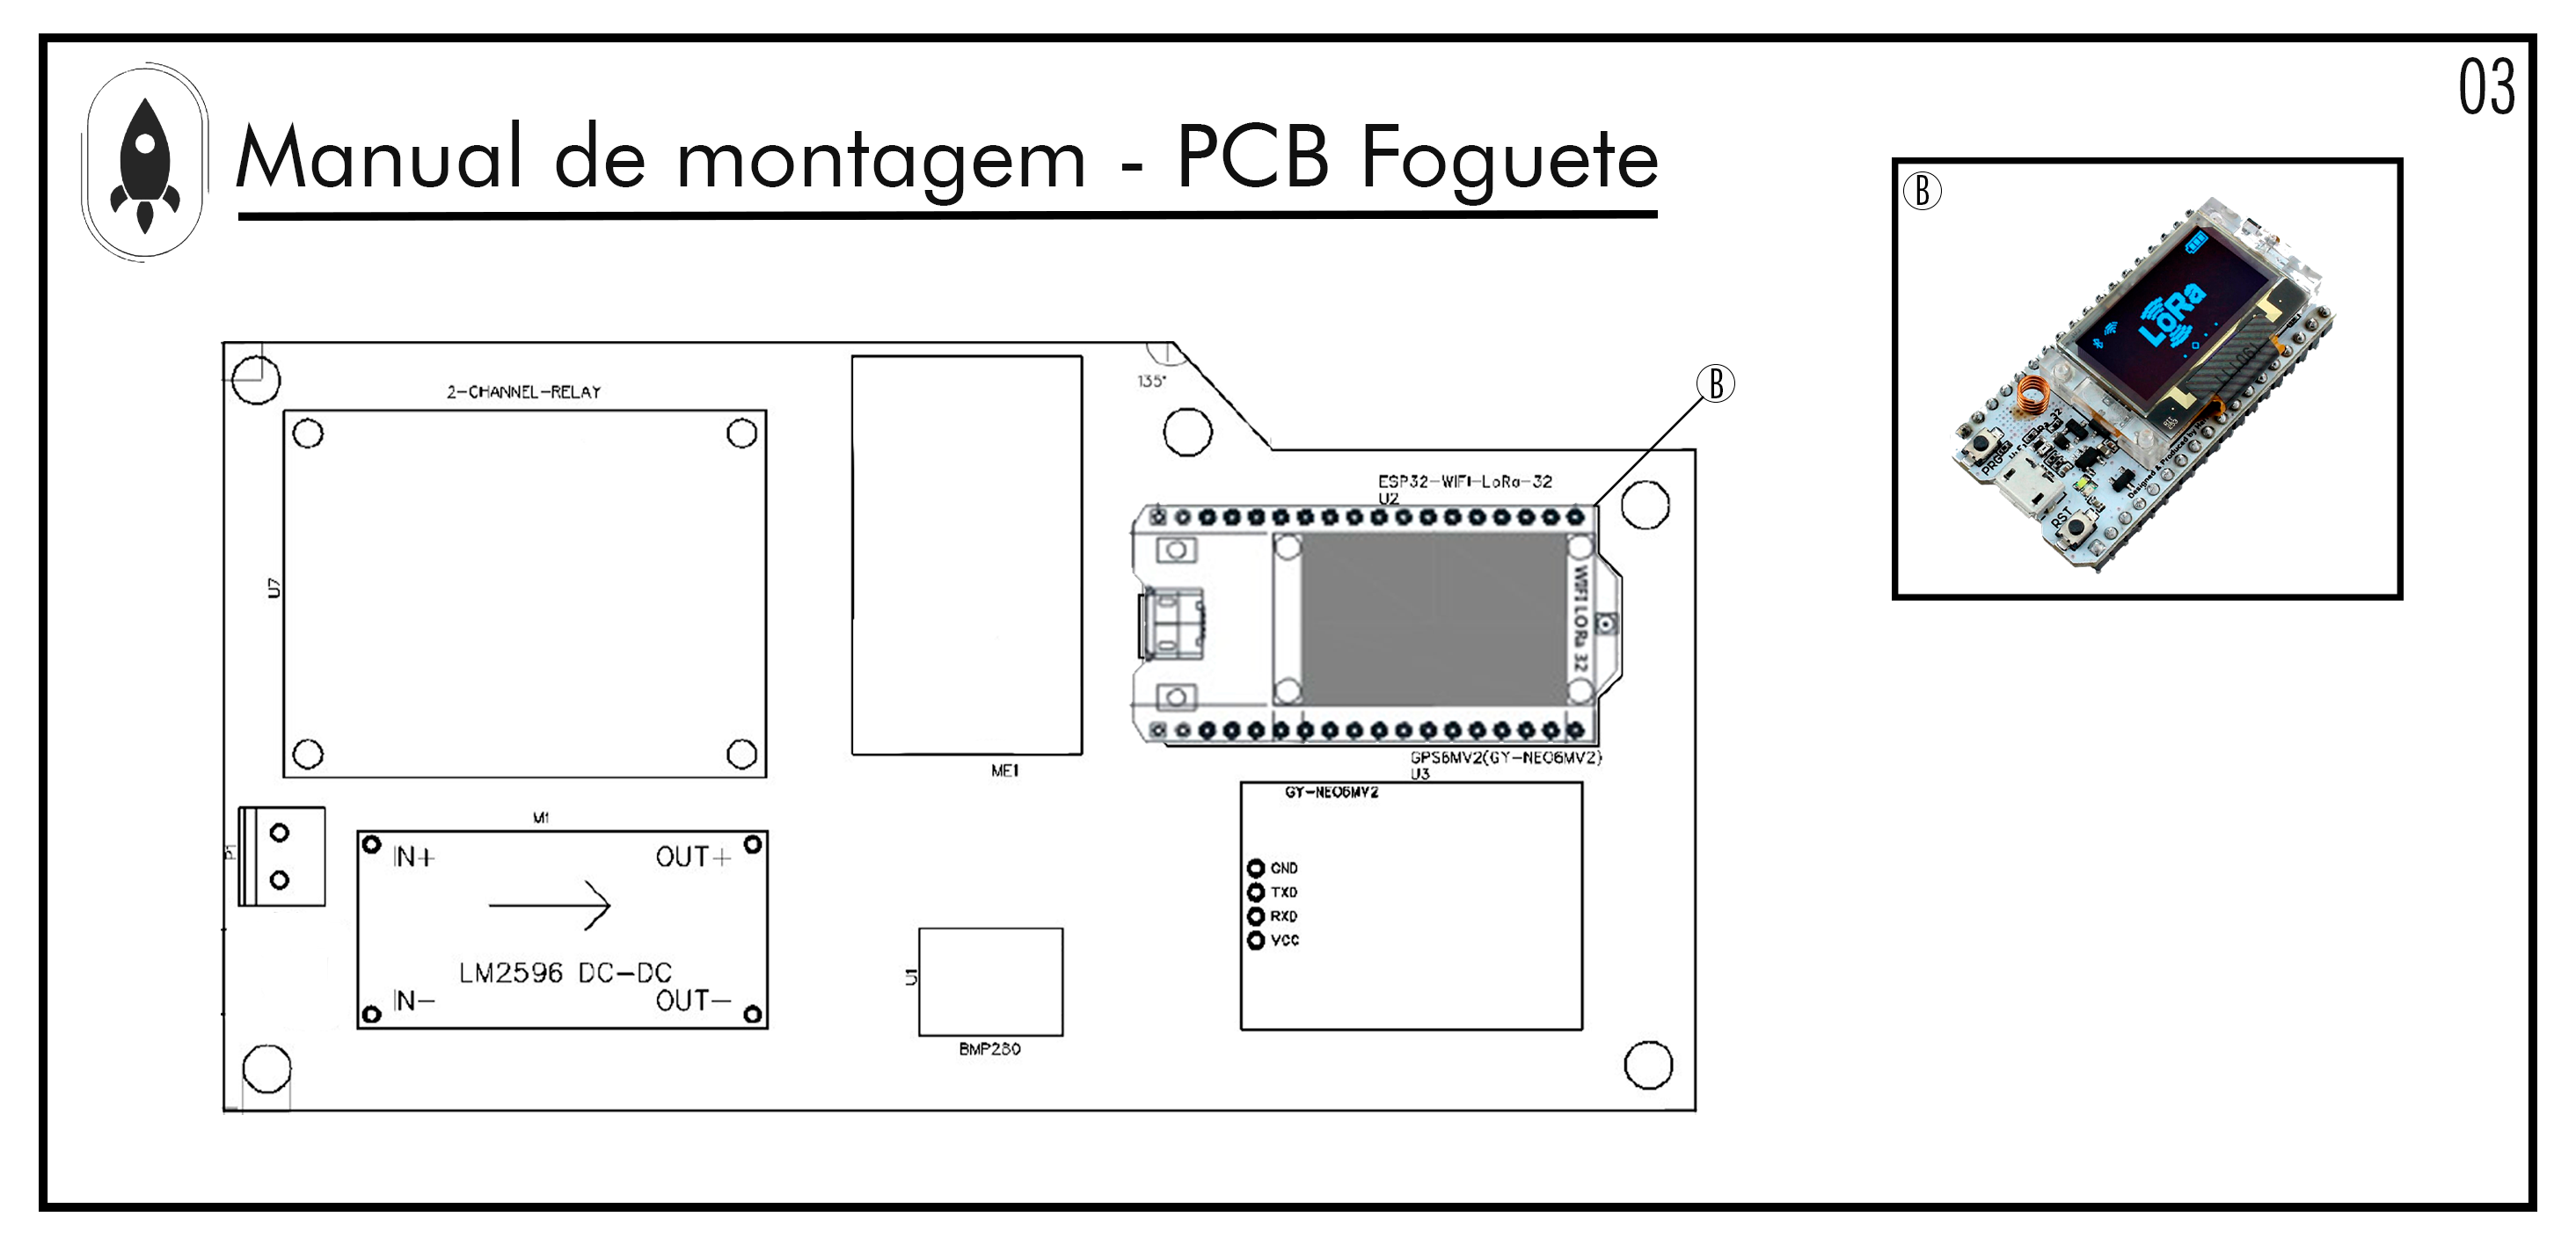
\includegraphics[width=\textwidth]{Figuras/FOGUETE/Pg-03---PL-02.png}
  \caption{ESP32 WiFi Lora.}
 %{ \footnotesize Fonte: Autores} 
  \label{fig:PCIFoguete LORA}
\end{figure}

\newpage

\par Pegue o componente 'C'(LM2596), encaixe-a na posição mostrada \ref{fig:PCIFoguete LM2596} e solde junto  a placa.
\begin{figure}[H]
  \centering
  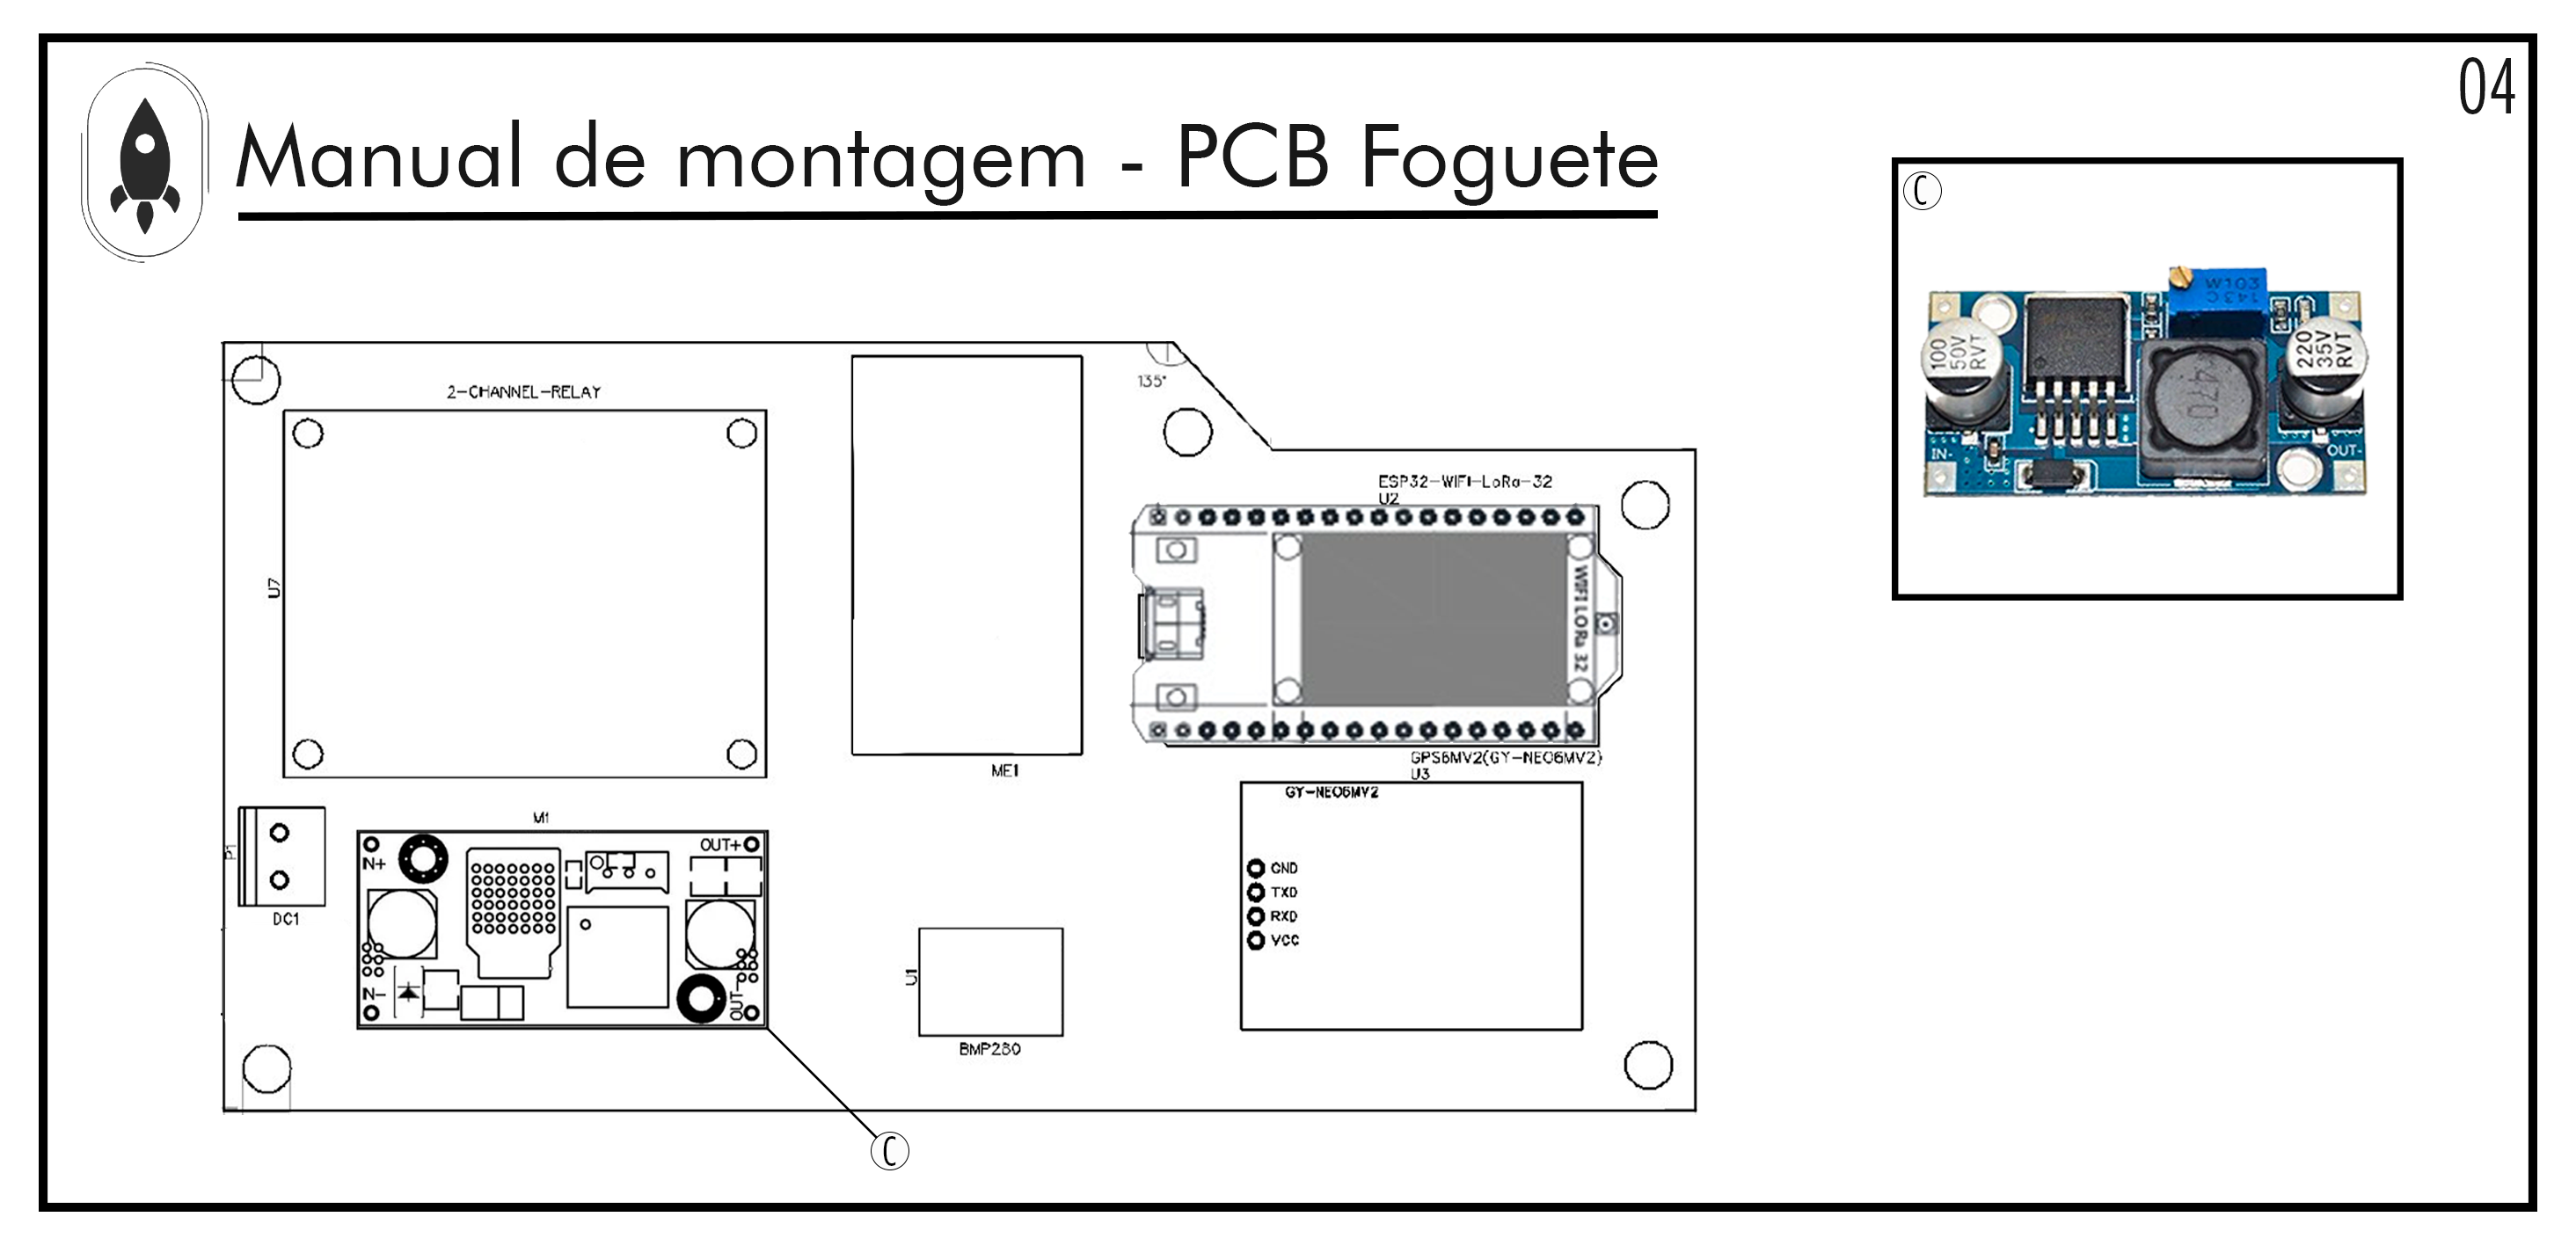
\includegraphics[width=\textwidth]{Figuras/FOGUETE/Pg-04---PL-02.png}
  \caption{LM2596.}
 %{ \footnotesize Fonte: Autores} 
  \label{fig:PCIFoguete LM2596}
\end{figure}


\par Pegue o componente 'D'(Conector fêmea jack P4 2,5mm), encaixe-a na posição mostrada \ref{fig:PCIFoguete jack P4} e solde junto a placa.
\begin{figure}[H]
  \centering
  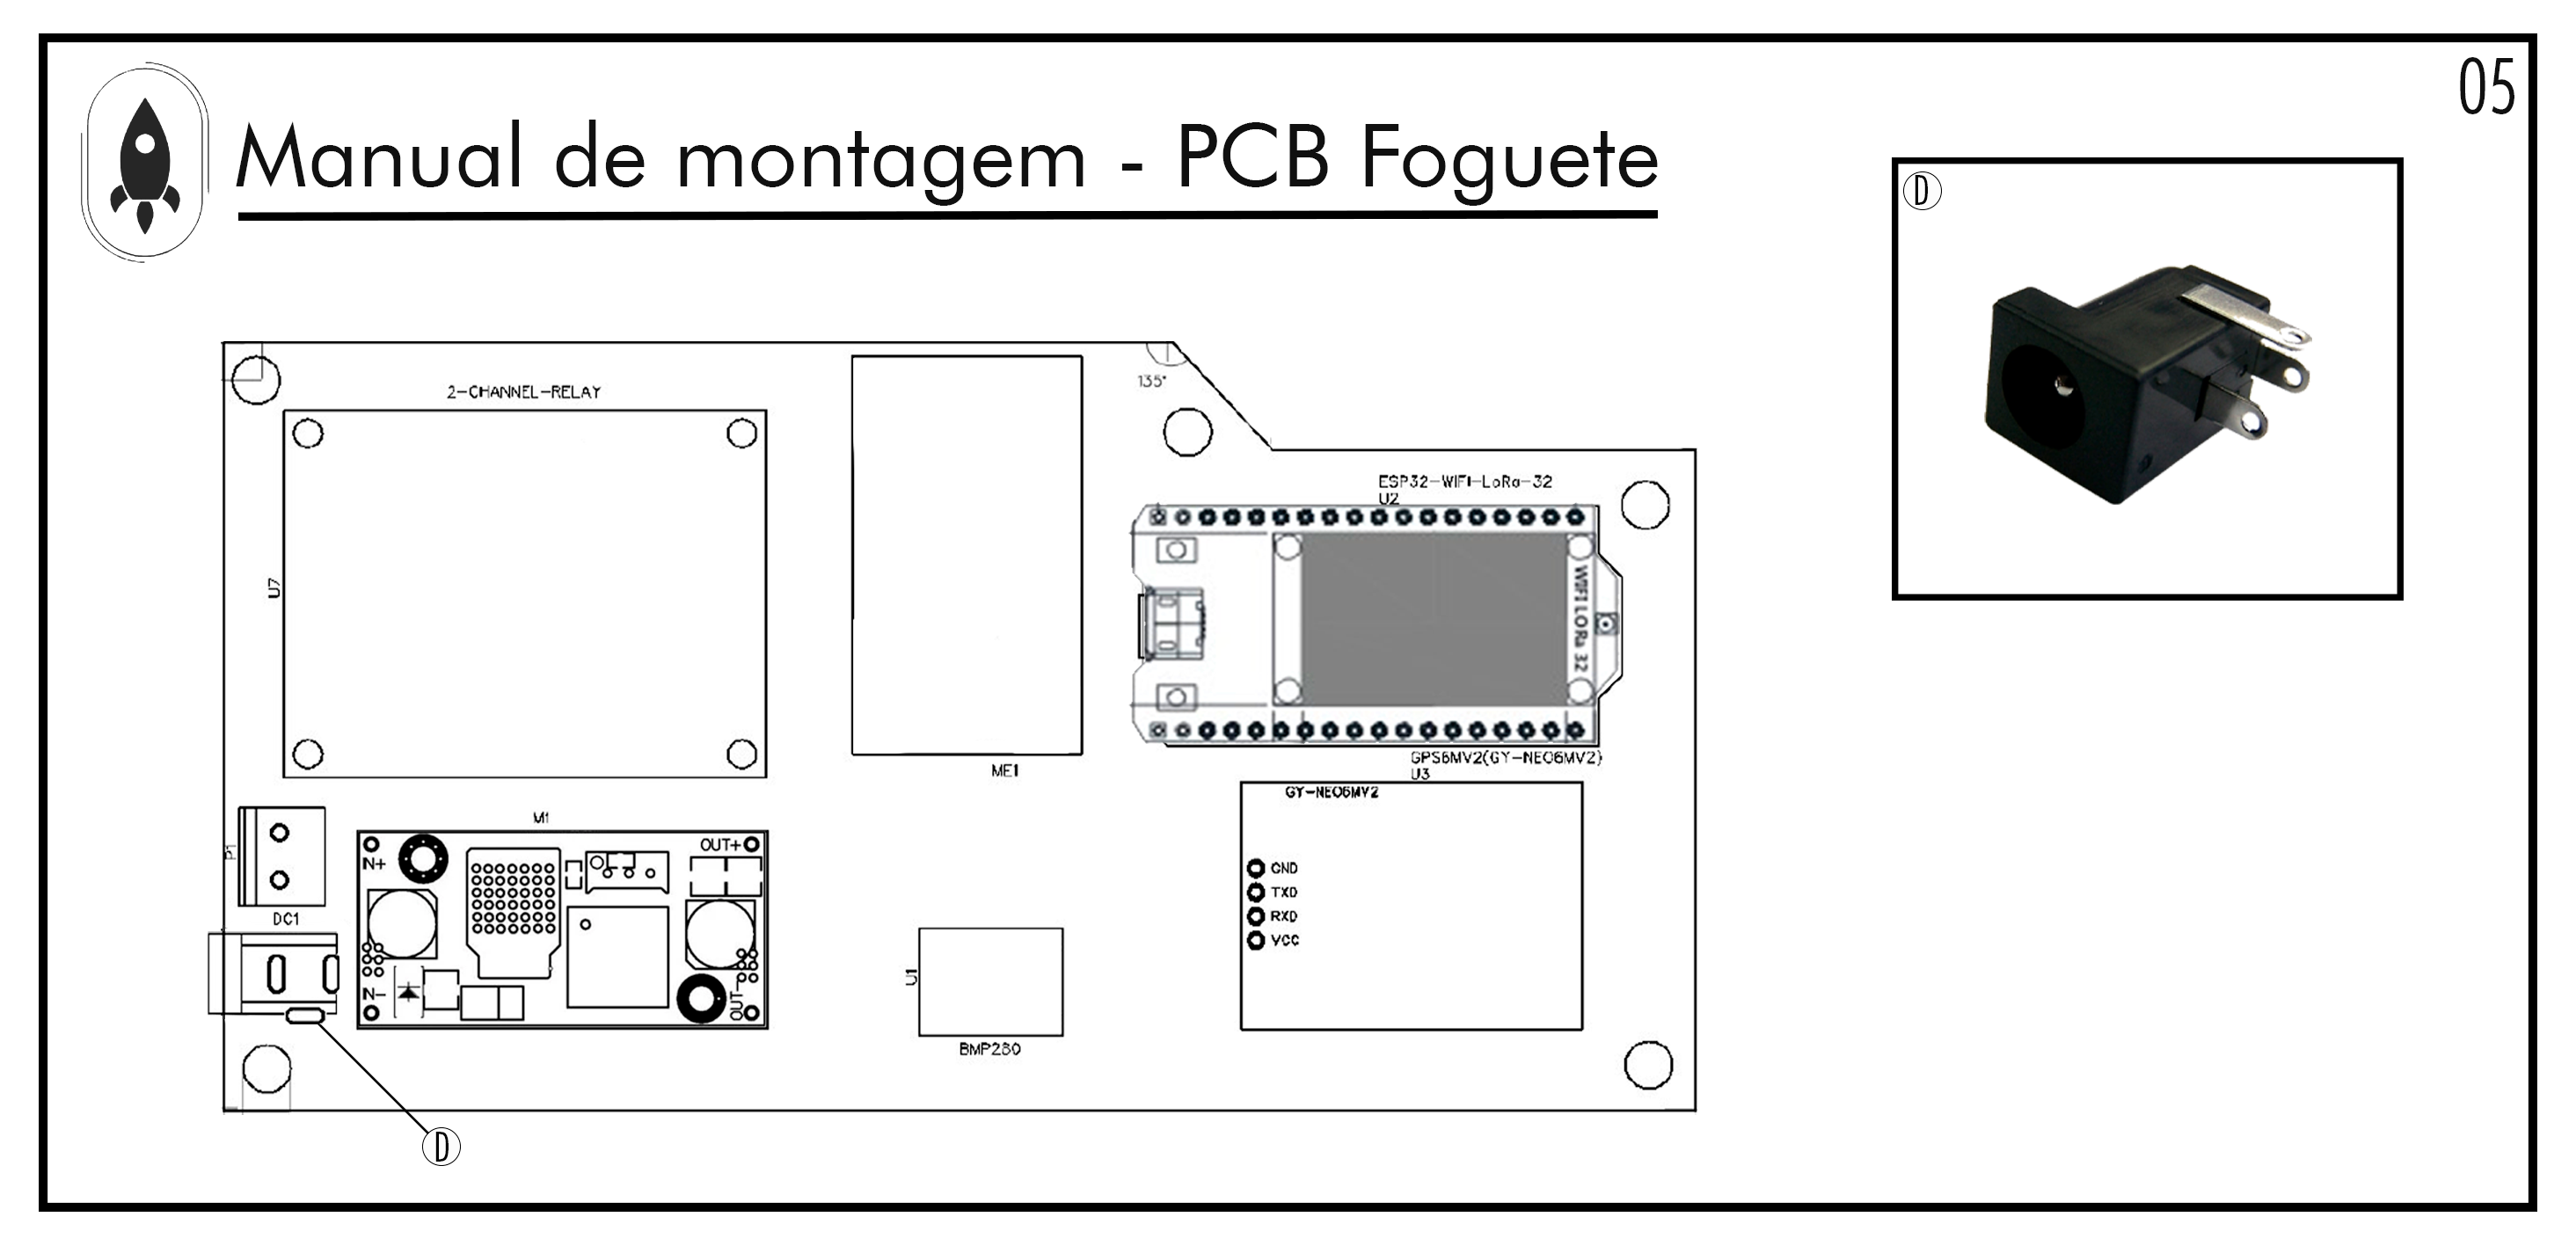
\includegraphics[width=\textwidth]{Figuras/FOGUETE/Pg-05---PL-02.png}
  \caption{Conector fêmea jack P4 2,5mm.}
 %{ \footnotesize Fonte: Autores} 
  \label{fig:PCIFoguete jack P4}
\end{figure}

\newpage

\par Pegue o componente 'E'(Sensor de Pressão e temperatura BMP280), encaixe-a na posição mostrada \ref{fig:PCIFoguete BMP280} e solde junto a placa.
\begin{figure}[H]
  \centering
  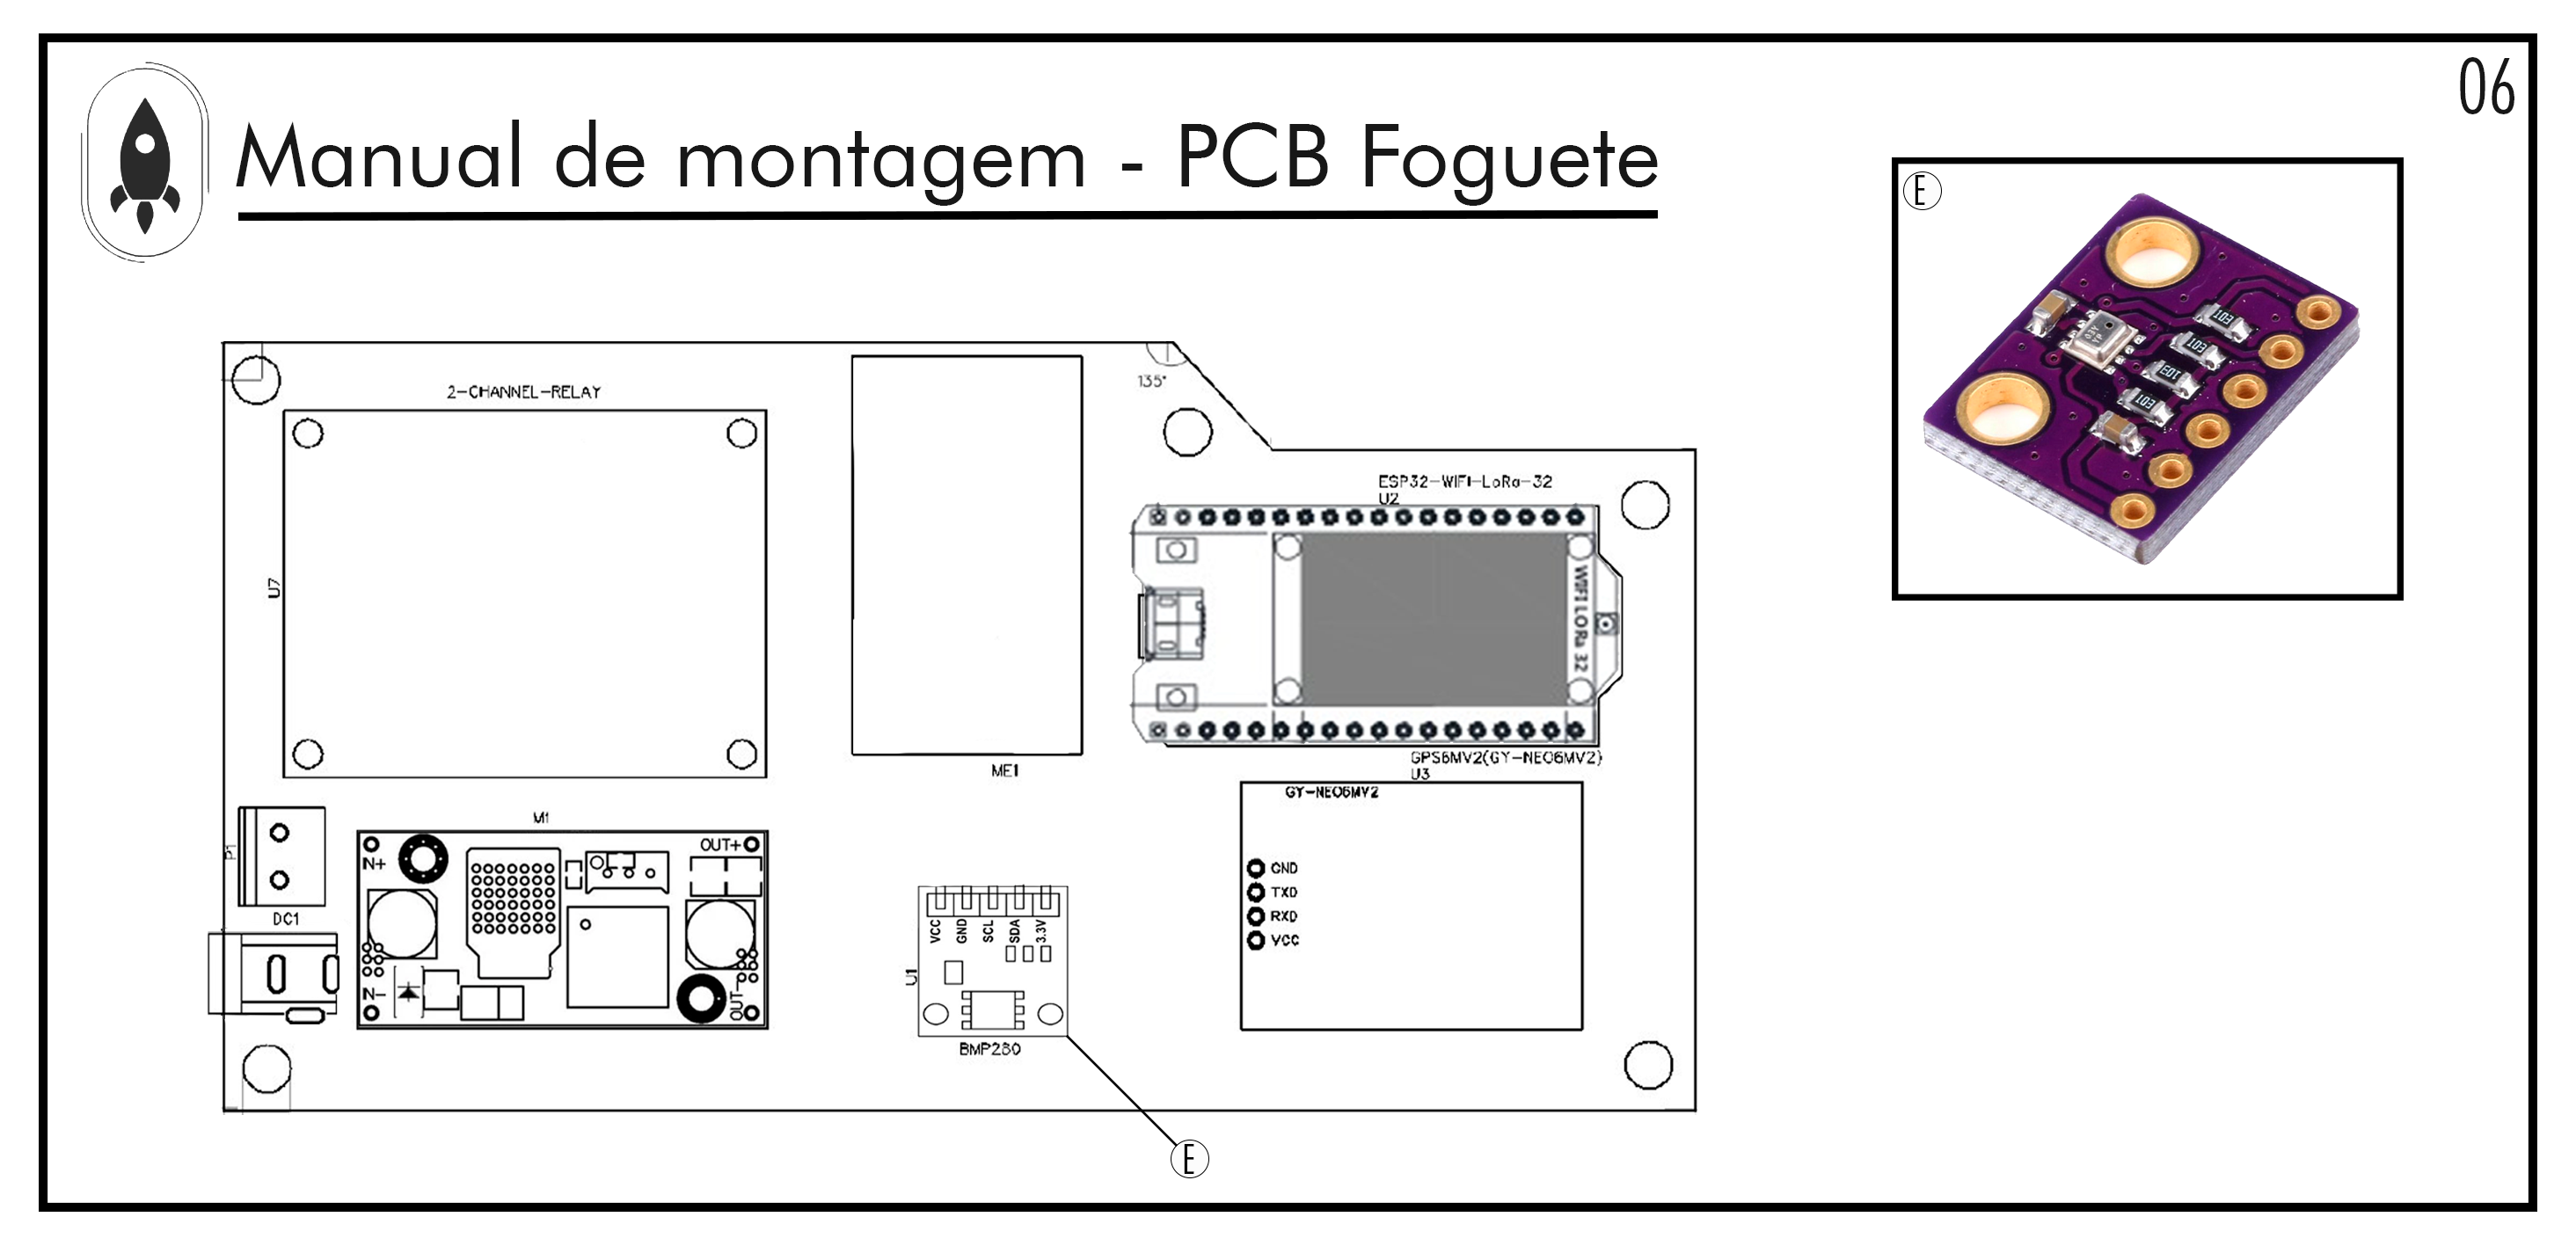
\includegraphics[width=\textwidth]{Figuras/FOGUETE/Pg-06---PL-02.png}
  \caption{Sensor de Pressão e temperatura BMP280.}
 %{ \footnotesize Fonte: Autores} 
  \label{fig:PCIFoguete BMP280}
\end{figure}


\par Pegue o componente 'F'(Módulo Relé 5V 2 Canais modelo SRD-05VDC-SL-C), encaixe-a na posição mostrada \ref{fig:PCIFoguete Relé} e solde junto  a placa.
\begin{figure}[H]
  \centering
  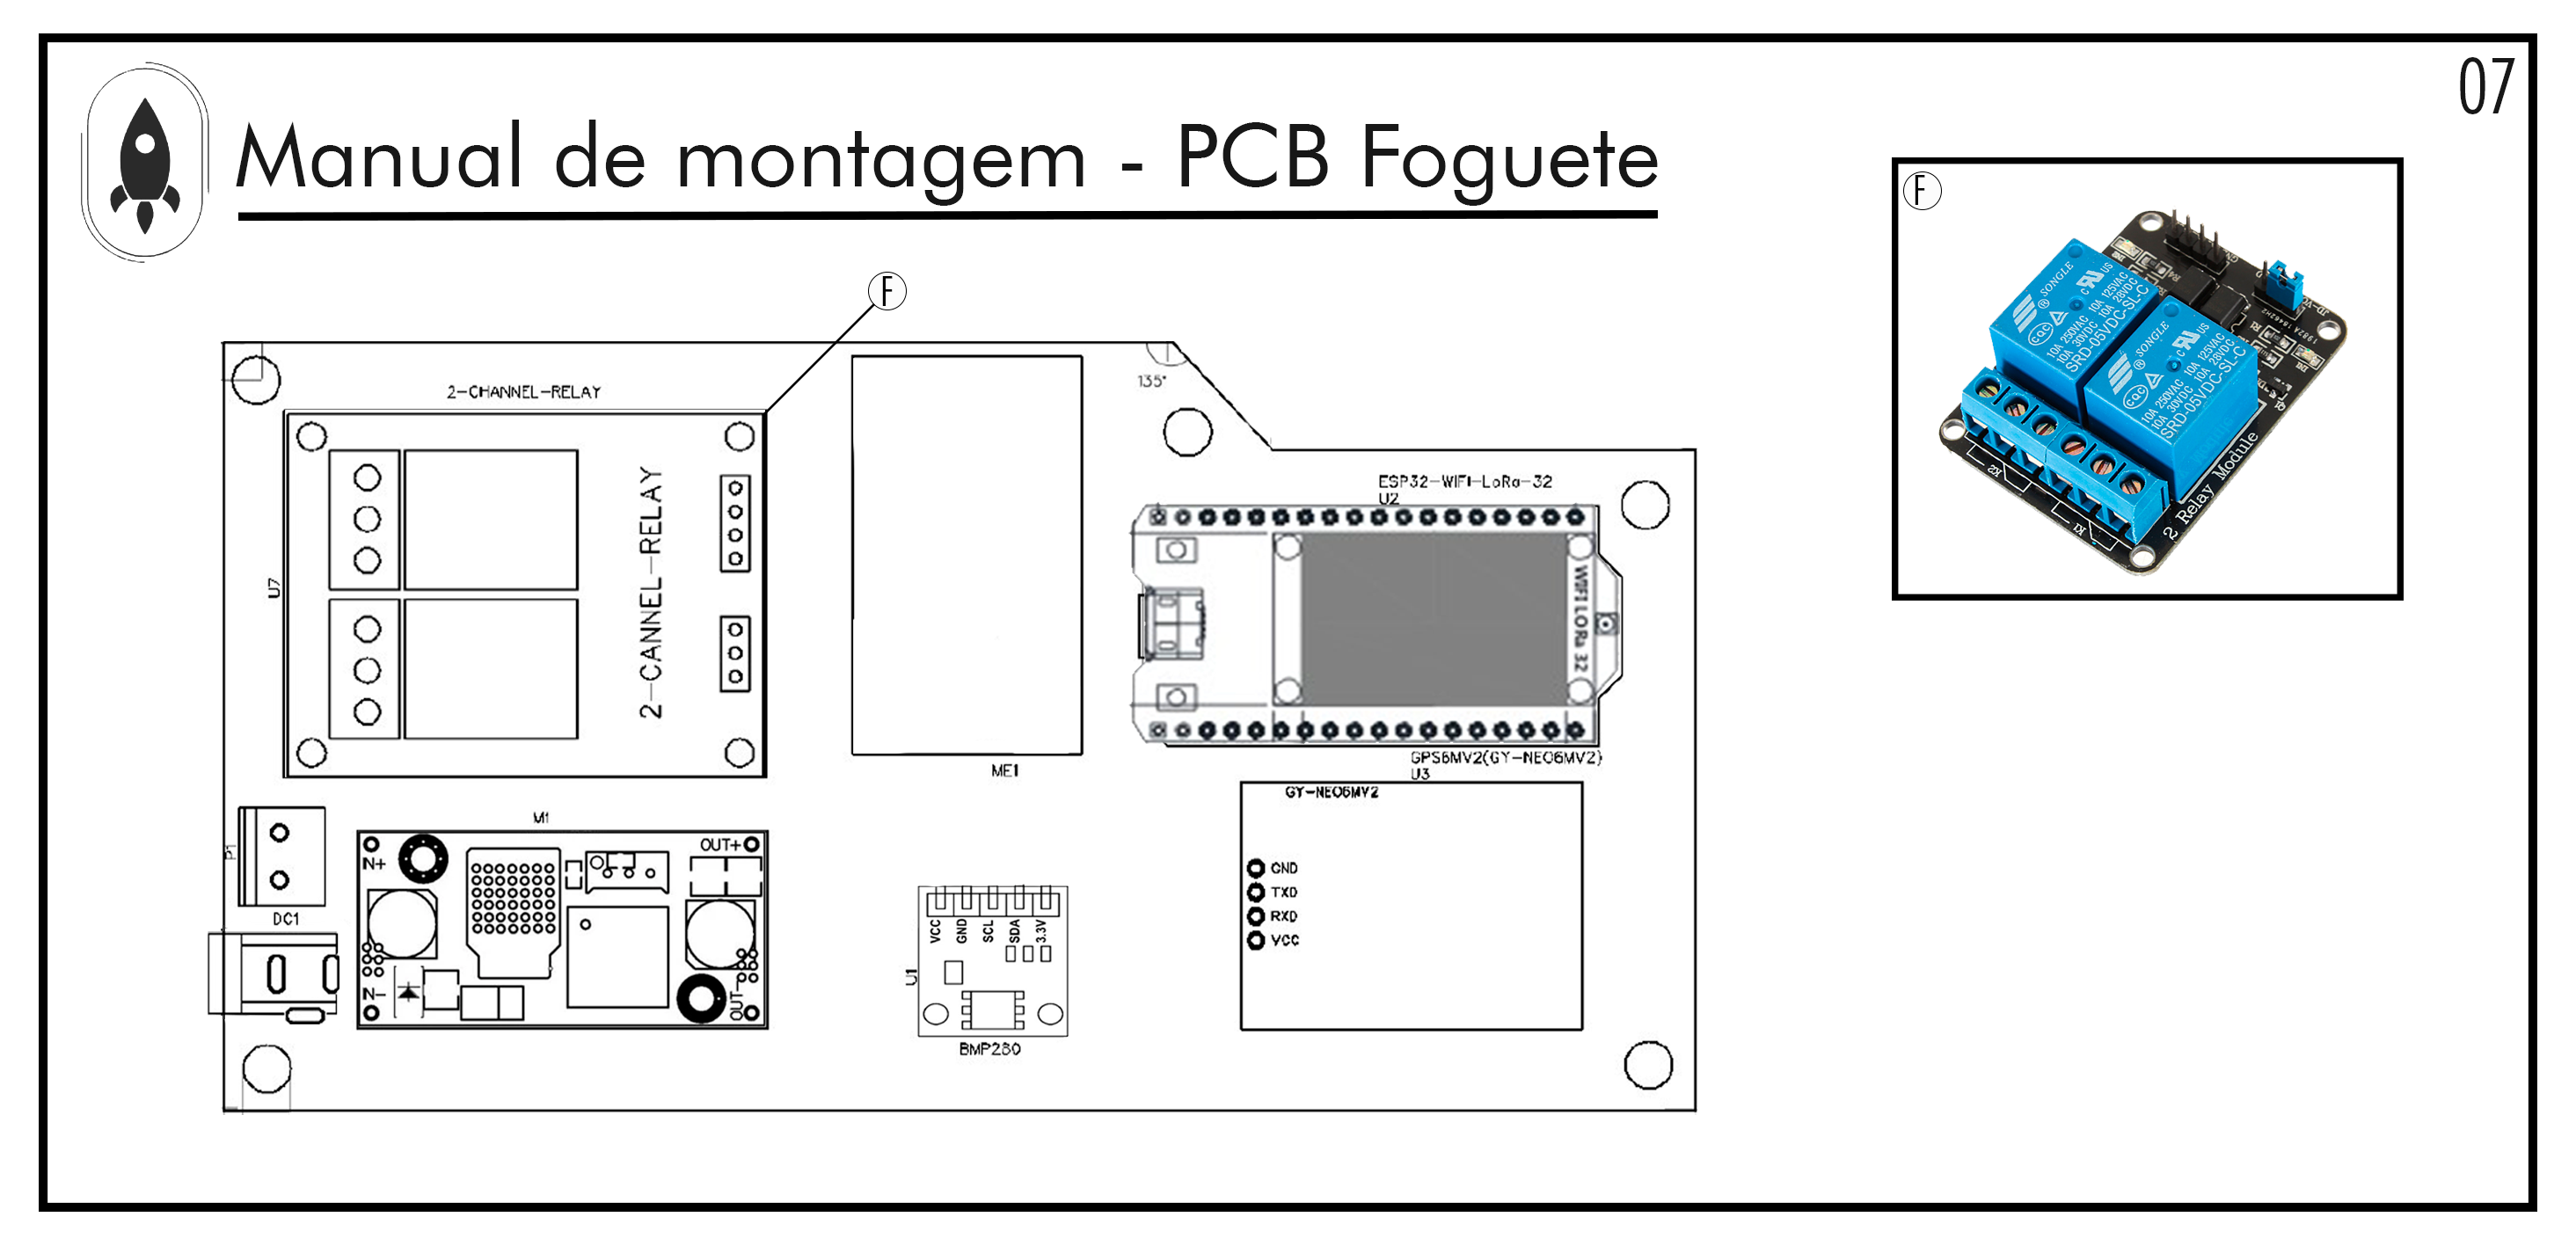
\includegraphics[width=\textwidth]{Figuras/FOGUETE/Pg-07---PL-02.png}
  \caption{Módulo Relé 5V 2 Canais modelo SRD-05VDC-SL-C.}
 %{ \footnotesize Fonte: Autores} 
  \label{fig:PCIFoguete Relé}
\end{figure}

\newpage

\par Pegue o componente 'G'(Módulo GPS GY-NEO6MV2), encaixe-a na posição mostrada \ref{fig:PCIBASE LORA} e solde junto a placa.
\begin{figure}[H]
  \centering
  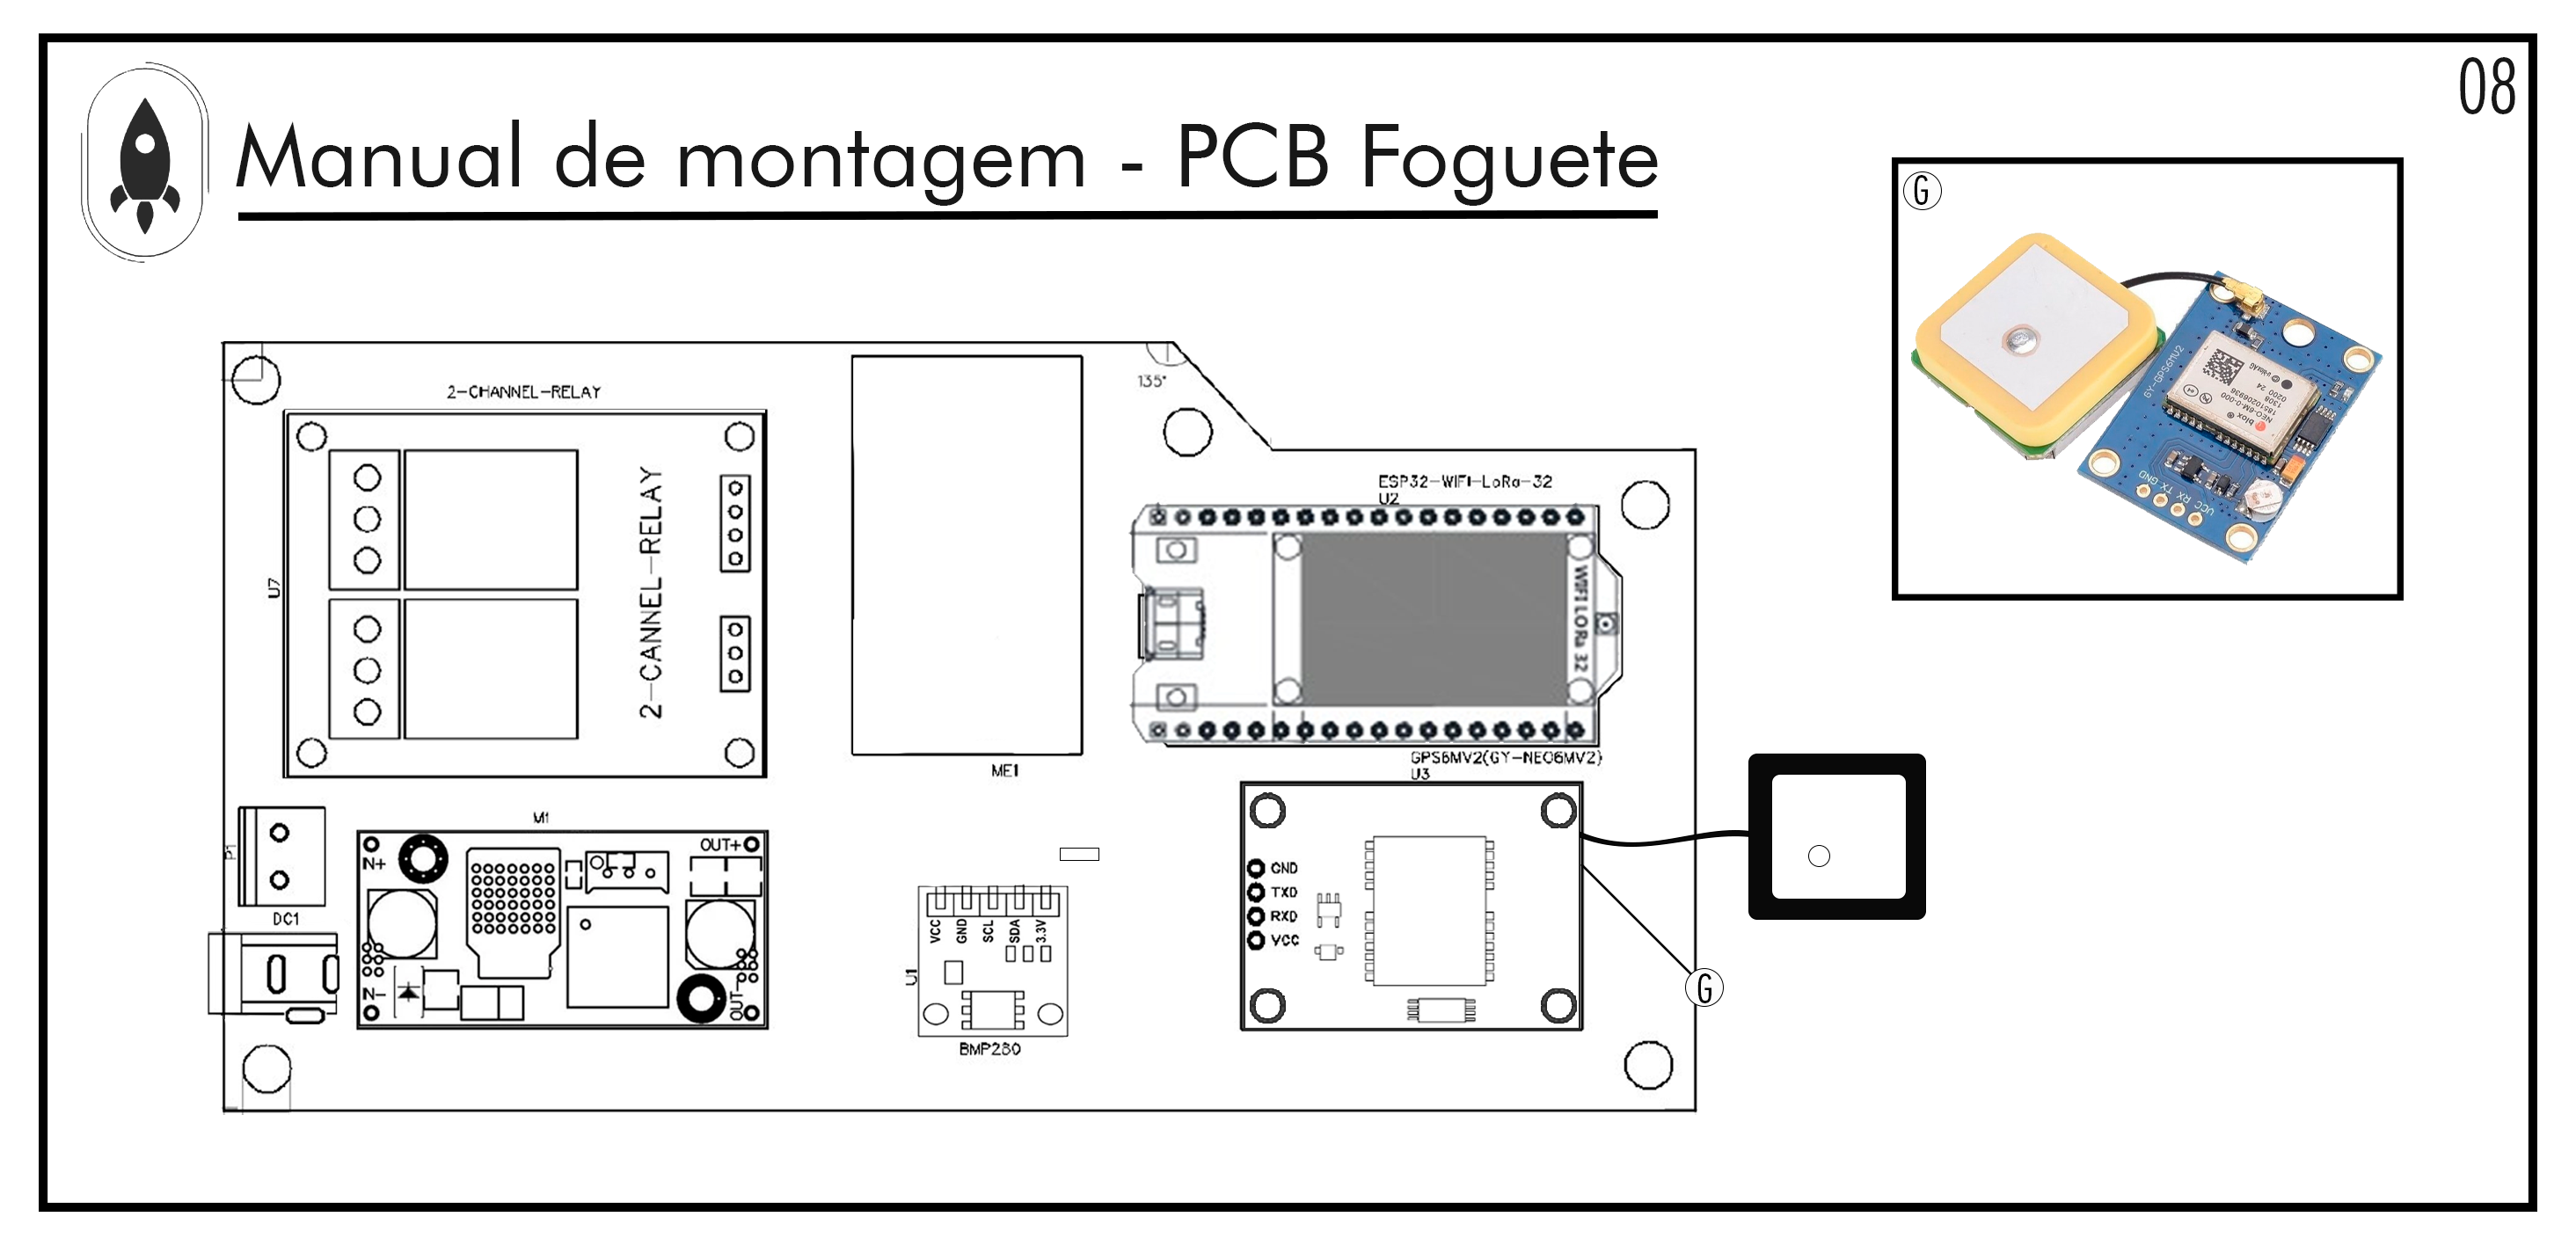
\includegraphics[width=\textwidth]{Figuras/FOGUETE/Pg-08---PL-02.png}
  \caption{Módulo GPS GY-NEO6MV2.}
 %{ \footnotesize Fonte: Autores} 
  \label{fig:PCIFoguete LORA}
\end{figure}


\par Pegue o componente 'H'(Módulo Cartão de Memoria), encaixe-a na posição mostrada \ref{fig:PCIFoguete MICRO SD CARD} e solde junto a placa.
\begin{figure}[H]
  \centering
  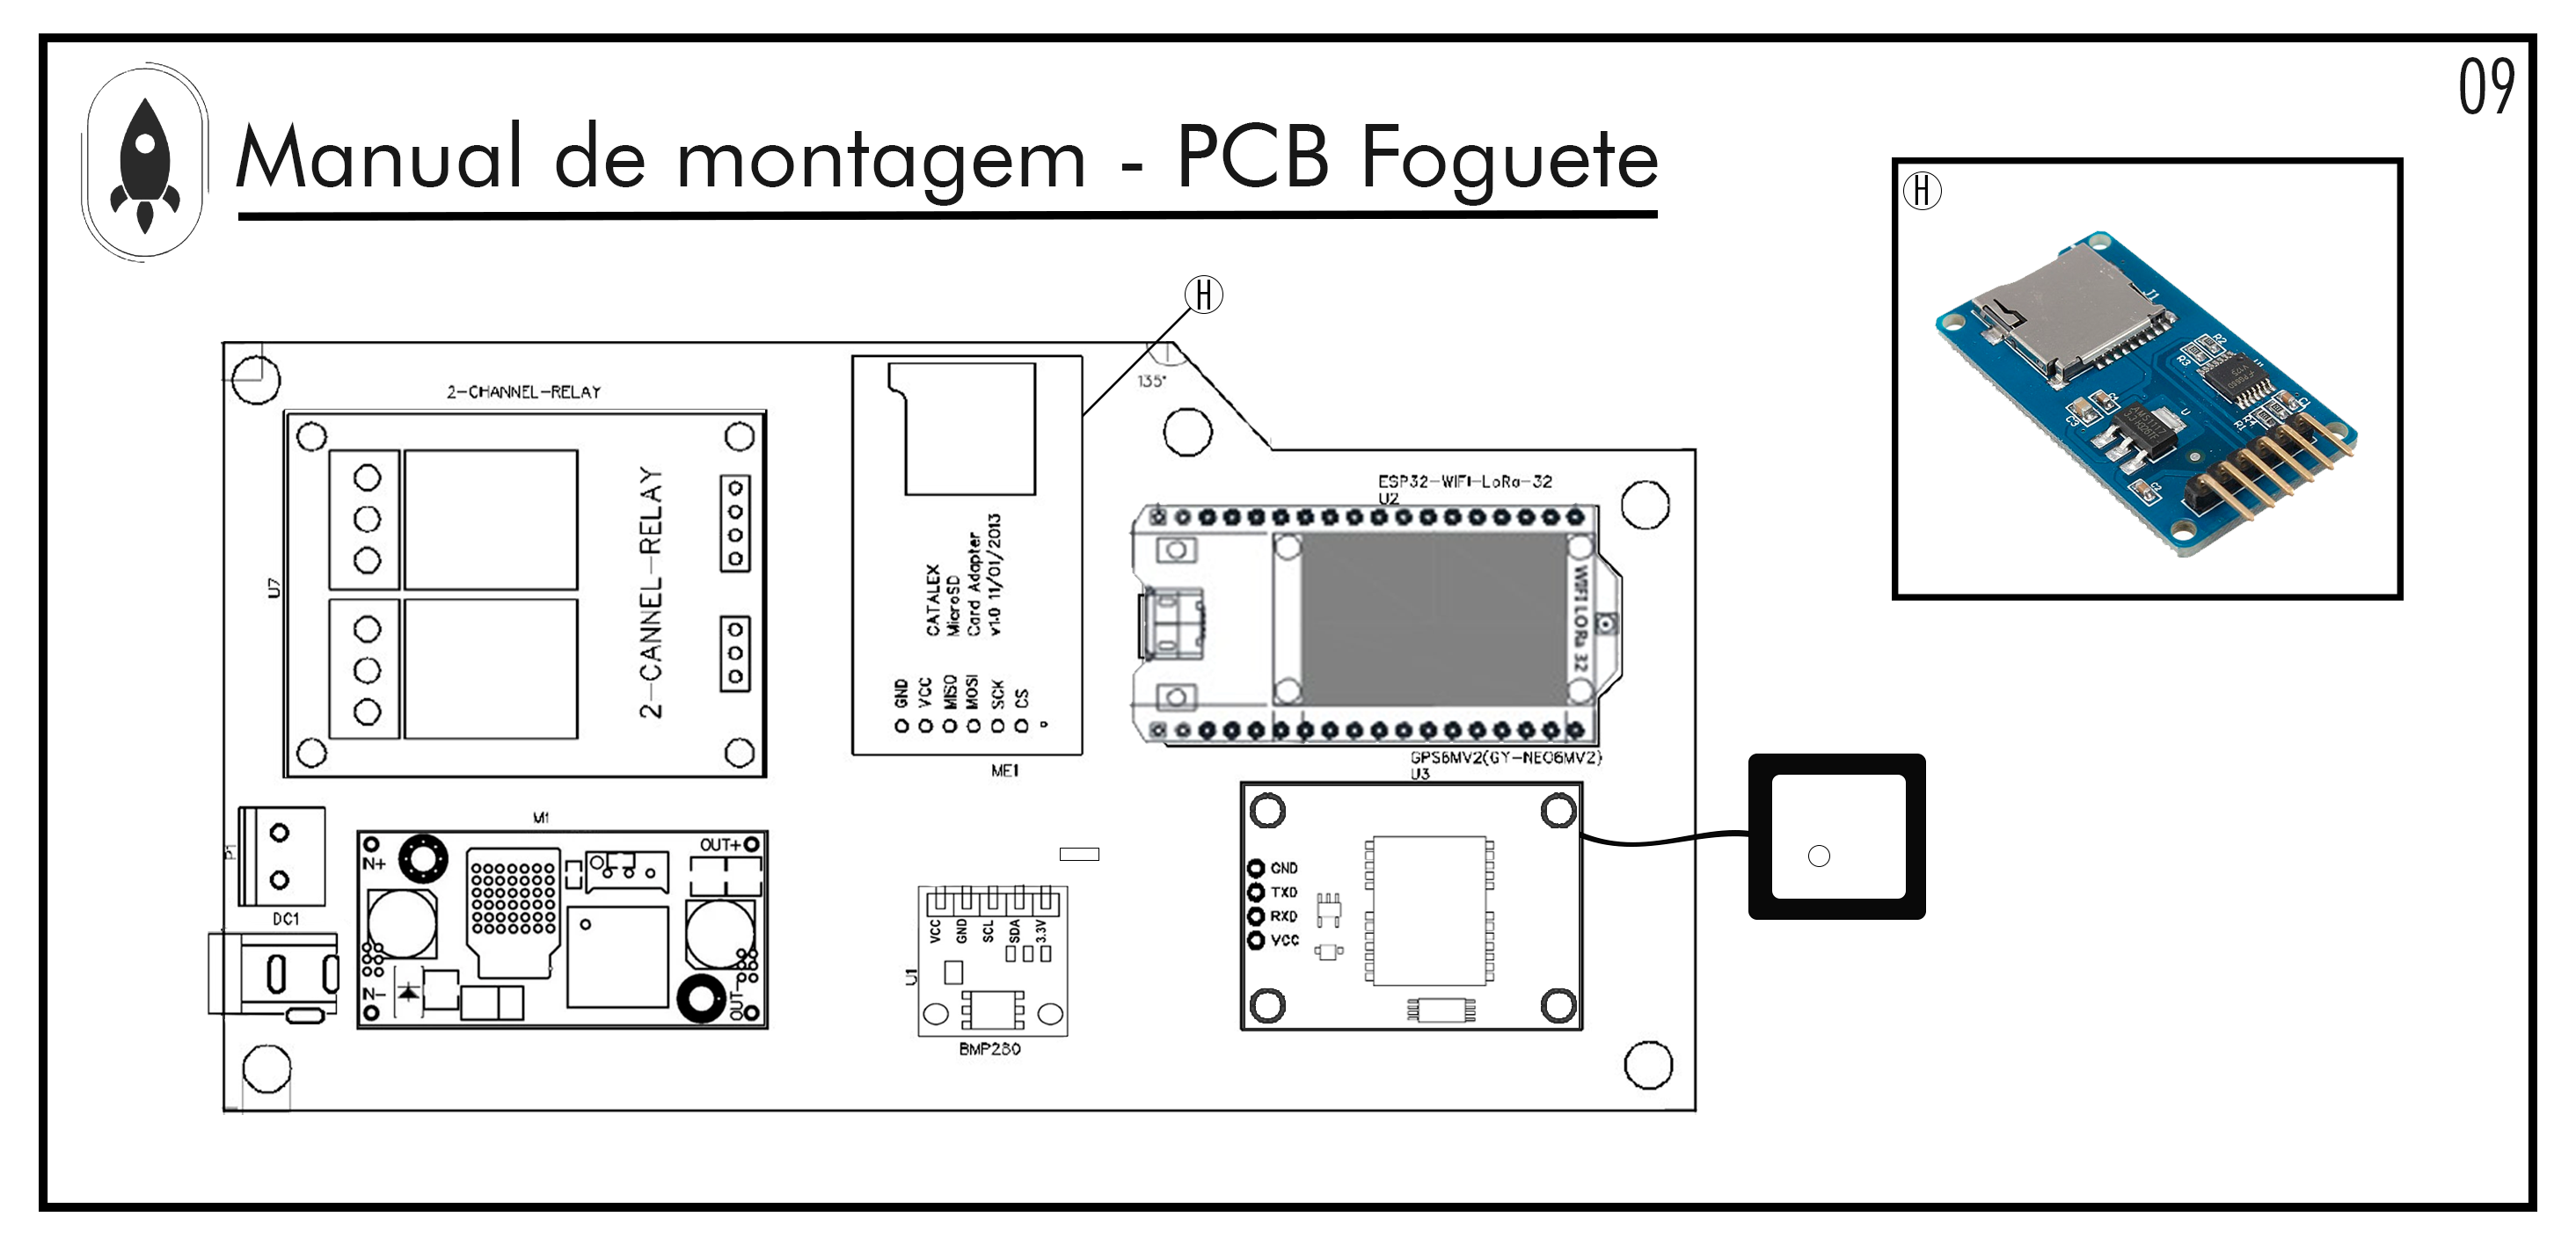
\includegraphics[width=\textwidth]{Figuras/FOGUETE/Pg-09---PL-02.png}
  \caption{Módulo Cartão de Memoria.}
 %{ \footnotesize Fonte: Autores} 
  \label{fig:PCIFoguete MICRO SD CARD}
\end{figure}

\newpage

\par Pegue o componente 'I'(Conector Borne KRE 2 Vias), encaixe-a na posição mostrada \ref{fig:PCIFoguete Borne} e solde junto a placa.
\begin{figure}[H]
  \centering
  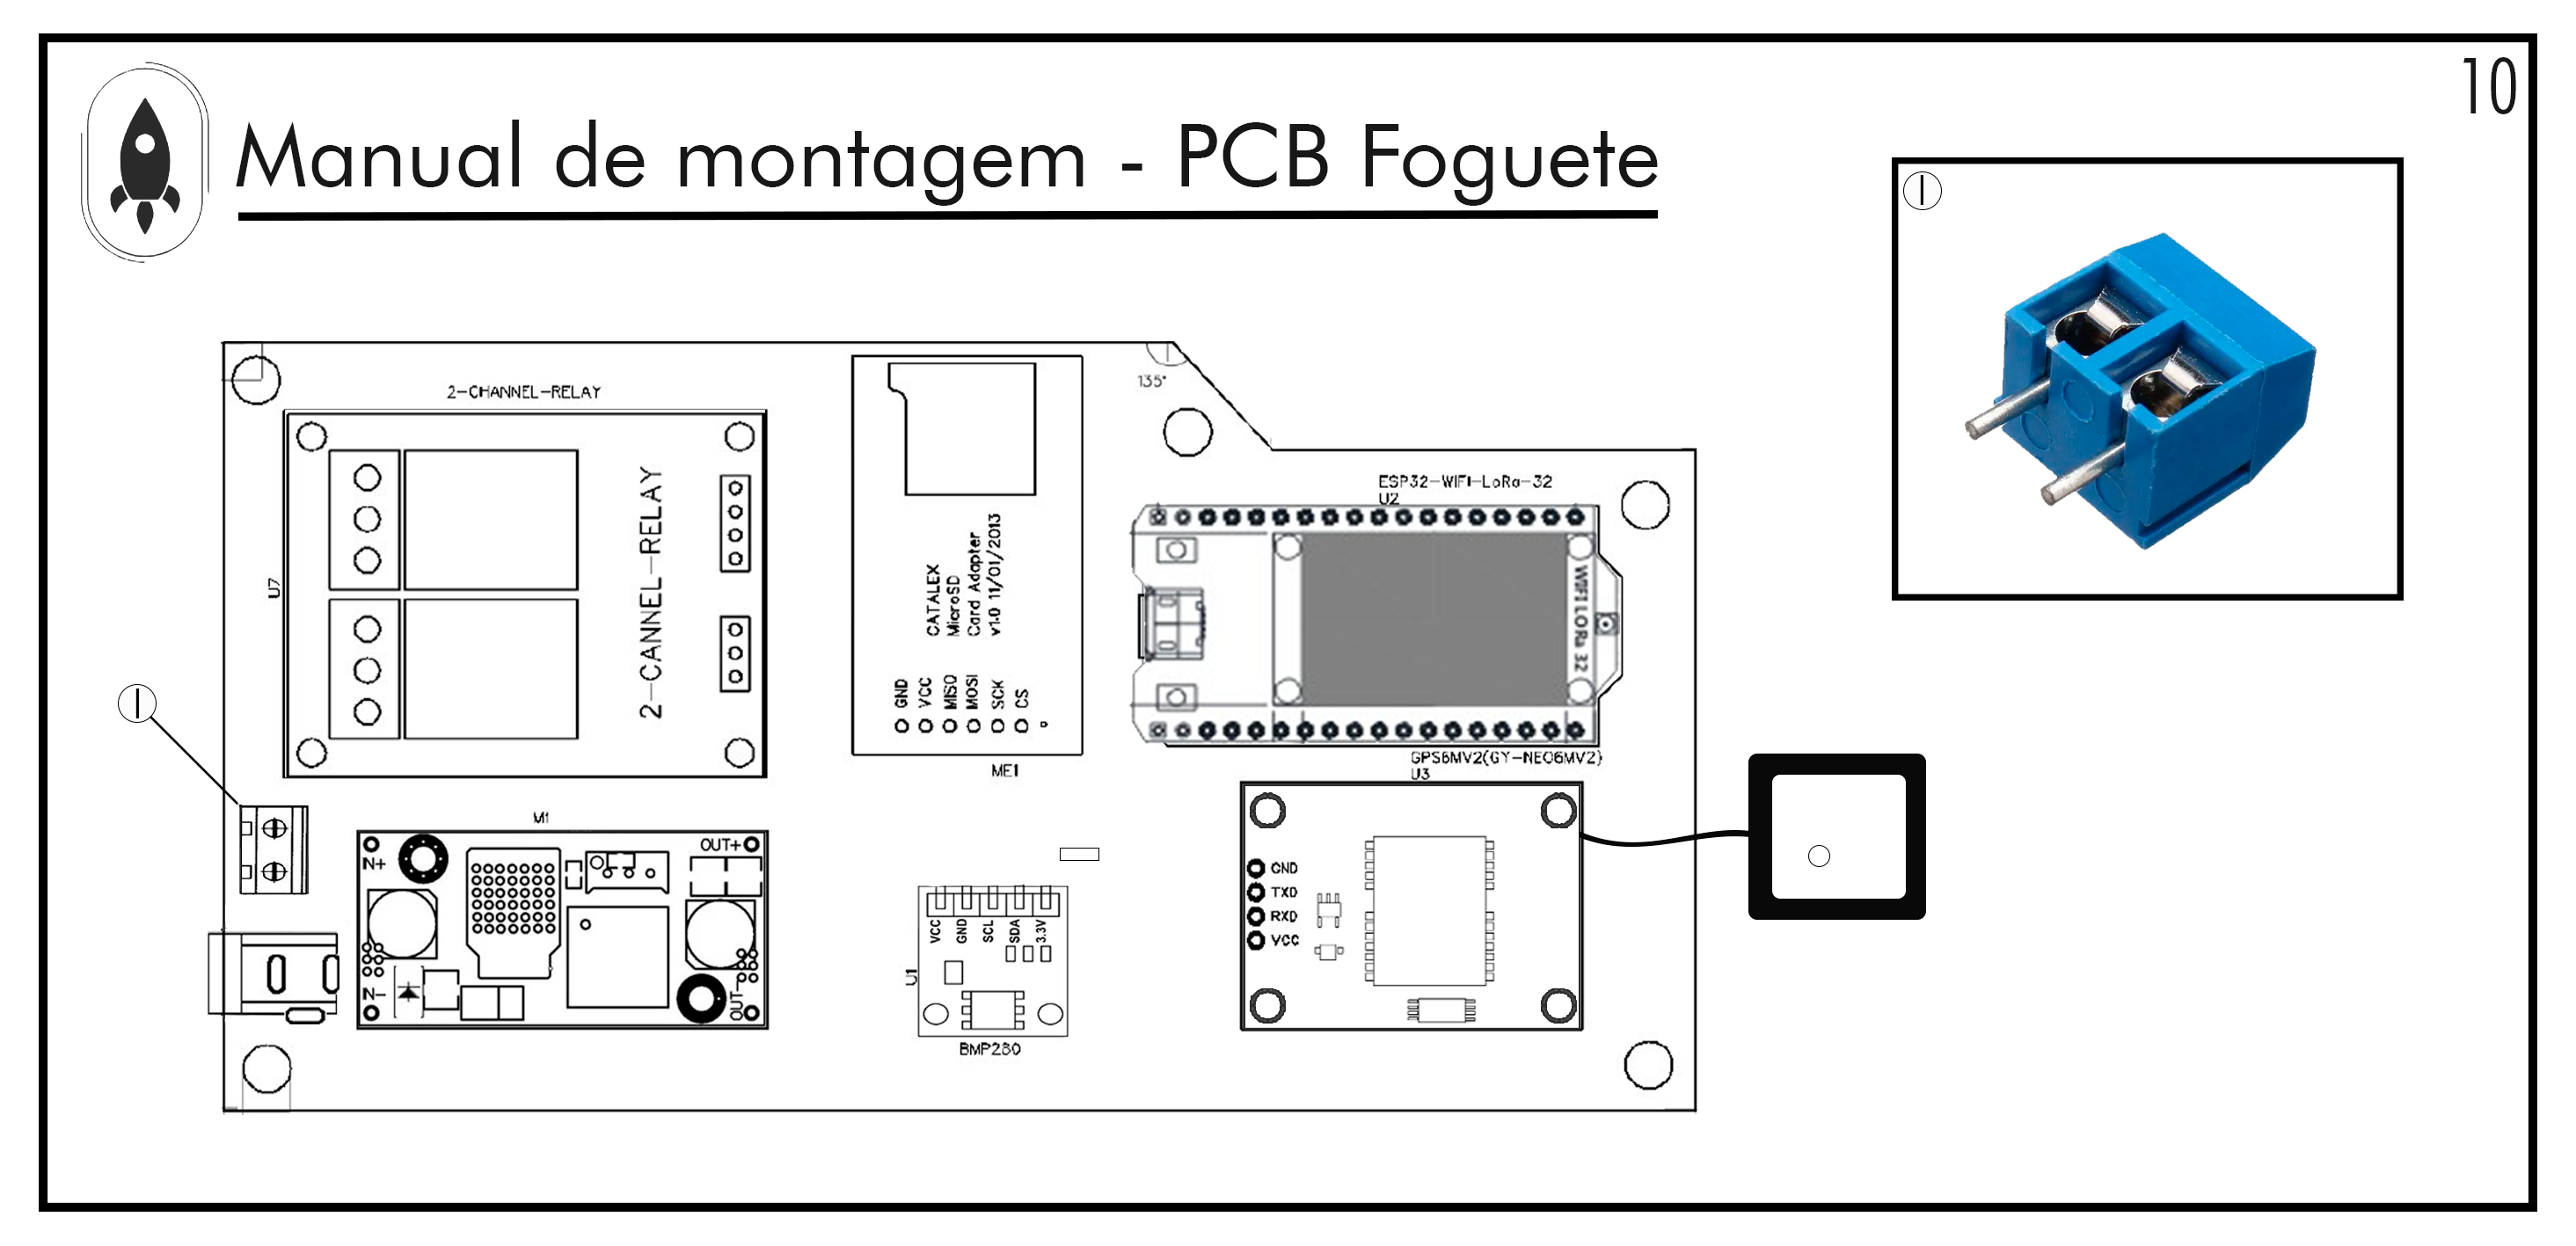
\includegraphics[width=\textwidth]{Figuras/FOGUETE/Pg-10---PL-02.png}
  \caption{Conector Borne KRE 2 Vias.}
 %{ \footnotesize Fonte: Autores} 
  \label{fig:PCIFoguete Borne}
\end{figure}
\par Para a fixação da placa em seu recipiente utilize os parafusos e a porca extensora, componentes 'J' e 'K' e siga as instruções da seção \ref{sec:fixação }.

\newpage

\subsection{Placas de Circuito Impresso-Maleta Interface do usuário}

\par Primeiramente é necessário ter em mão todos os componentes para sua montagem \ref{fig:Lista de materiasi MALETA}.

\subsubsection{Lista de Materiais}

\par Primeiramente é necessário ter em mão todos os componentes para sua montagem \ref{fig:Lista de materiais MALETA1}.

\begin{table}[H]
\centering
\begin{tabular}{|m{1.9cm} |m{1.8cm} |m{7.3cm}|m{4cm}|}
\hline
\begin{center}Identificador\end{center} &\begin{center} Quantidade\end{center} & \begin{center}Componente\end{center} &\begin{center} Part Number\end{center} \\\hline
A&01 &  PCI- Maleta  & -  \\\hline

B&02 & Conector Adaptador Plug P4 Macho com Borne &  P4 Macho F0503 \\\hline
C&01 & Micro Usb V8 Macho & J5415\\\hline
D&01 & Plug Hdmi Macho & Hdmi Macho \\\hline
E&01 & Conector Jack J4 DC Fêmea &  Jack Fêmea  \\\hline
F&01 & Chave Gangorra 2 Polos Mini  & Kcd11-101   \\\hline
G &01&Lora Esp32 Sx1278 Com Display  Oled Wifi bluetooth 915mhz& Sx1278 \\\hline
H & 01 & NVIDIA Jetson Nano Developer Kit  & 945-13450-0000-100\\\hline 
I & 01 &Placa controladora   & PCB800099-V.9  \\\hline 
J& 01 &  Conversor DC-DC Step Down-LM2596 (12~5V)
& LM2596 \\\hline
K &01& Display LCD 9 polegadas  & Lcd 9" TMOEC \\\hline
L& 01&Mini  Teclado  slim  com  Touchpad & -  \\\hline
\end{tabular}
\caption{Lista de componentes}
\end{table}


\subsubsection{Instruções}

\begin{figure}[H]
  \centering
  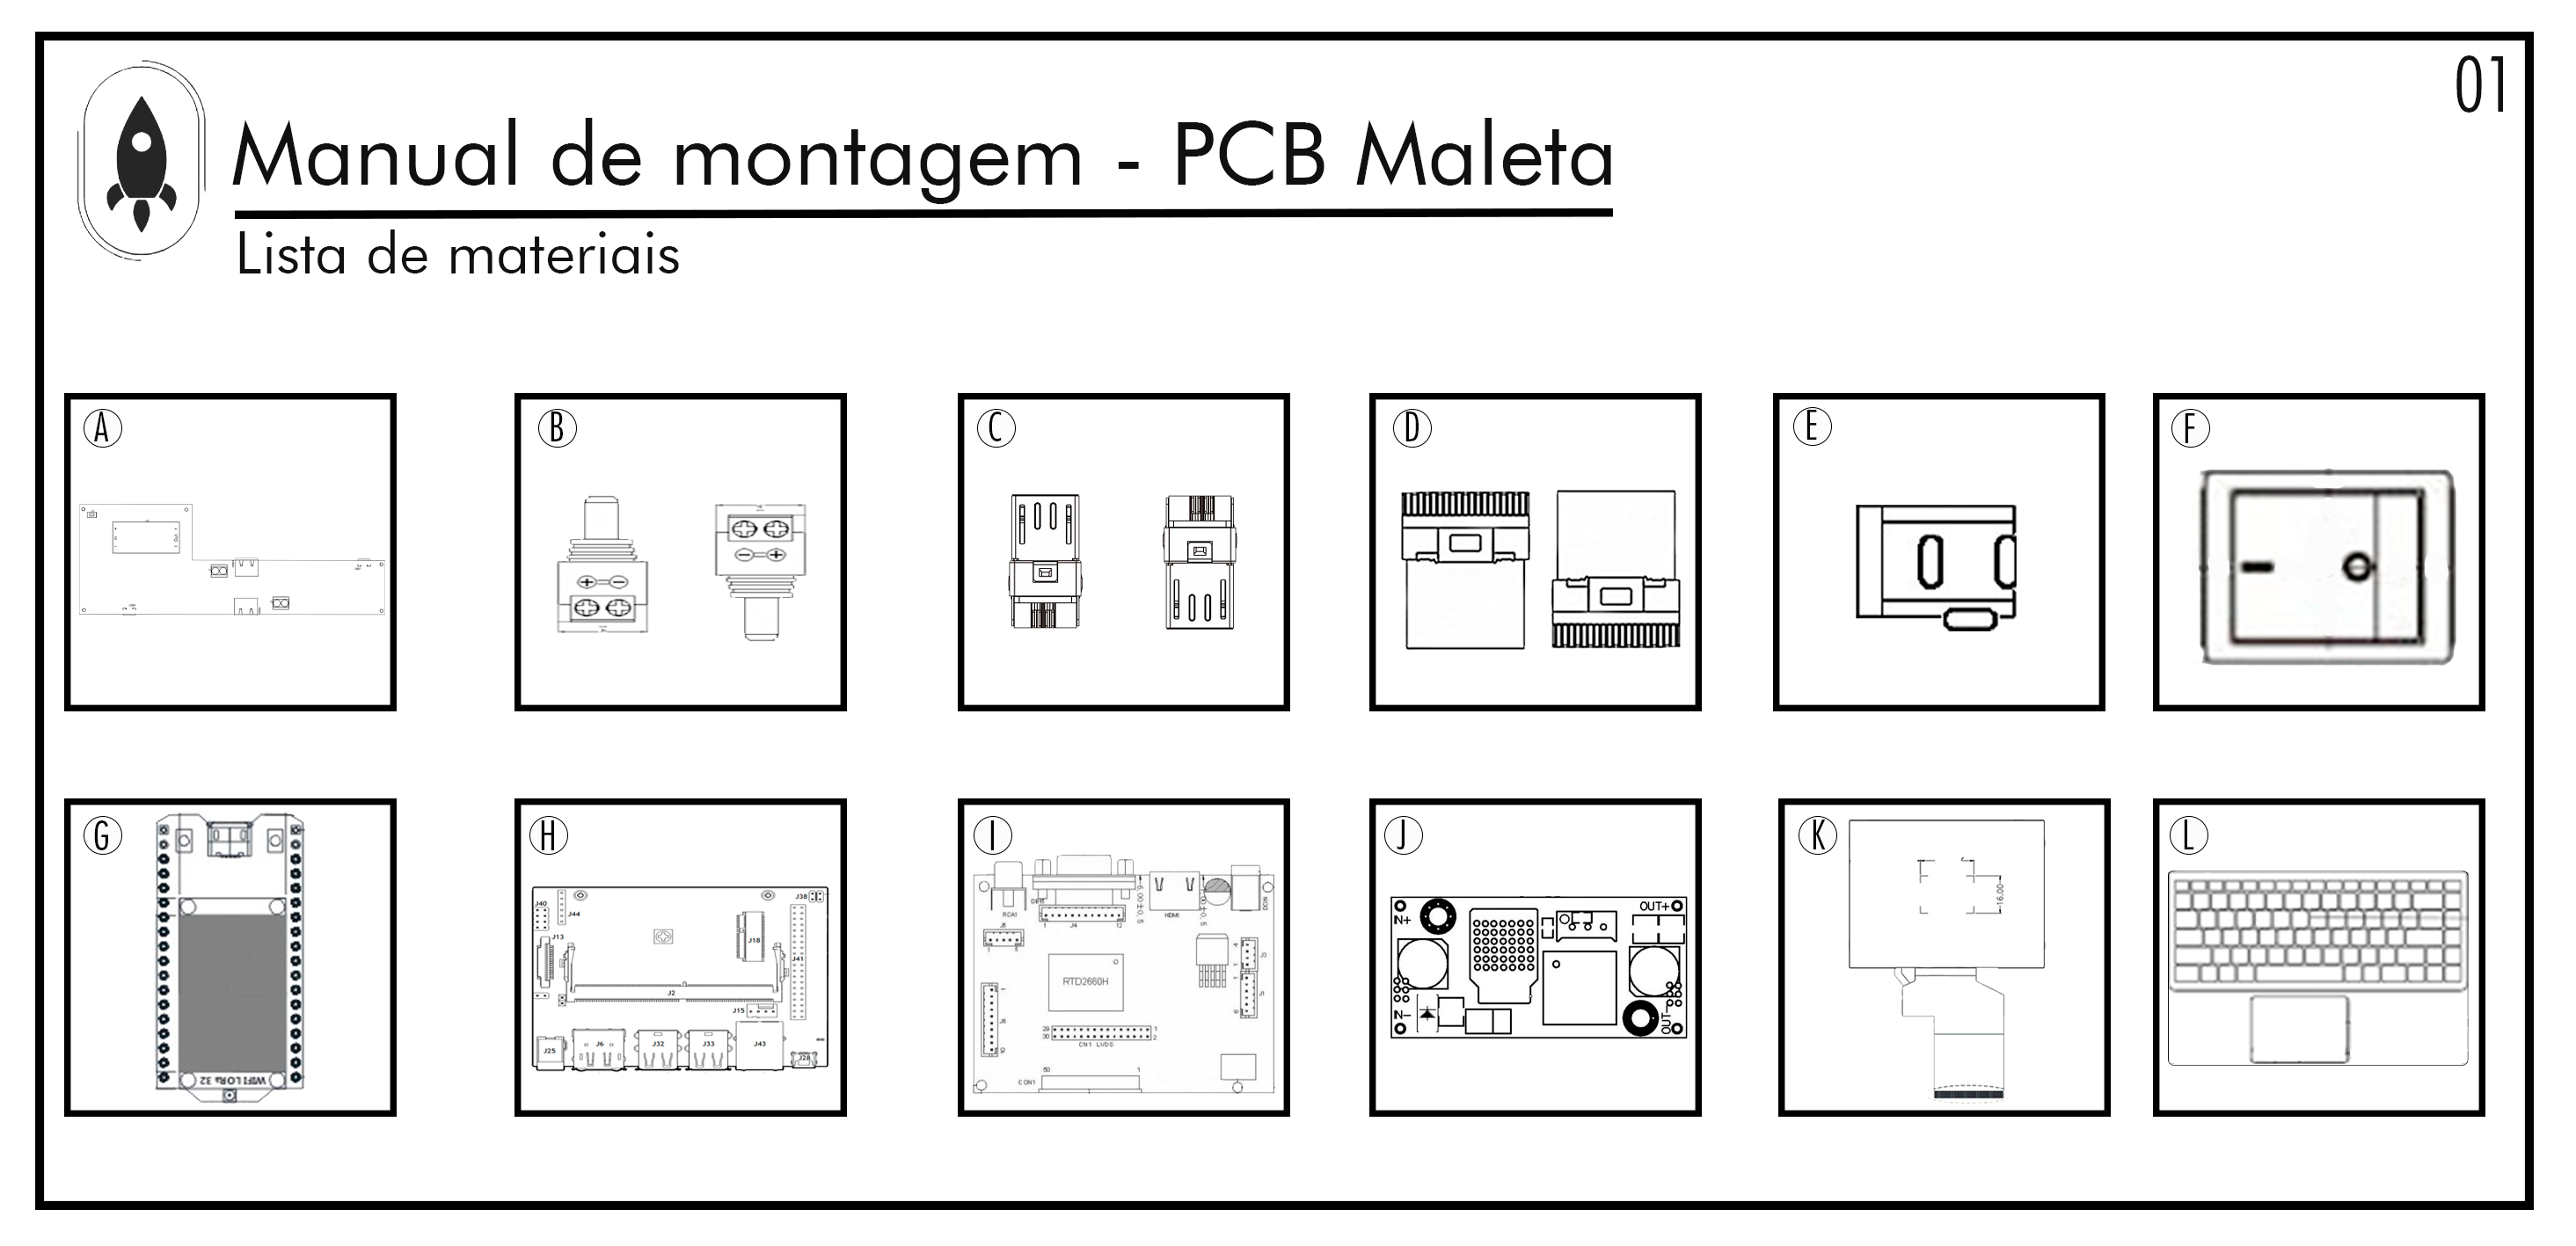
\includegraphics[width=\textwidth]{Figuras/MALETA/Pg-01---PL-01.png}
  \caption{Lista de Materiais.} 
 %{ \footnotesize Fonte: Autores} 
  \label{fig:Lista de materiais MALETA1}
\end{figure}


 \par Com todos os componentes em mãos, pegue componente 'A'(PCI-MALETA) prepare-a para soldagem dos componentes passando uma fina camada de solda nos pads da PCI.

\begin{figure}[H]
  \centering
  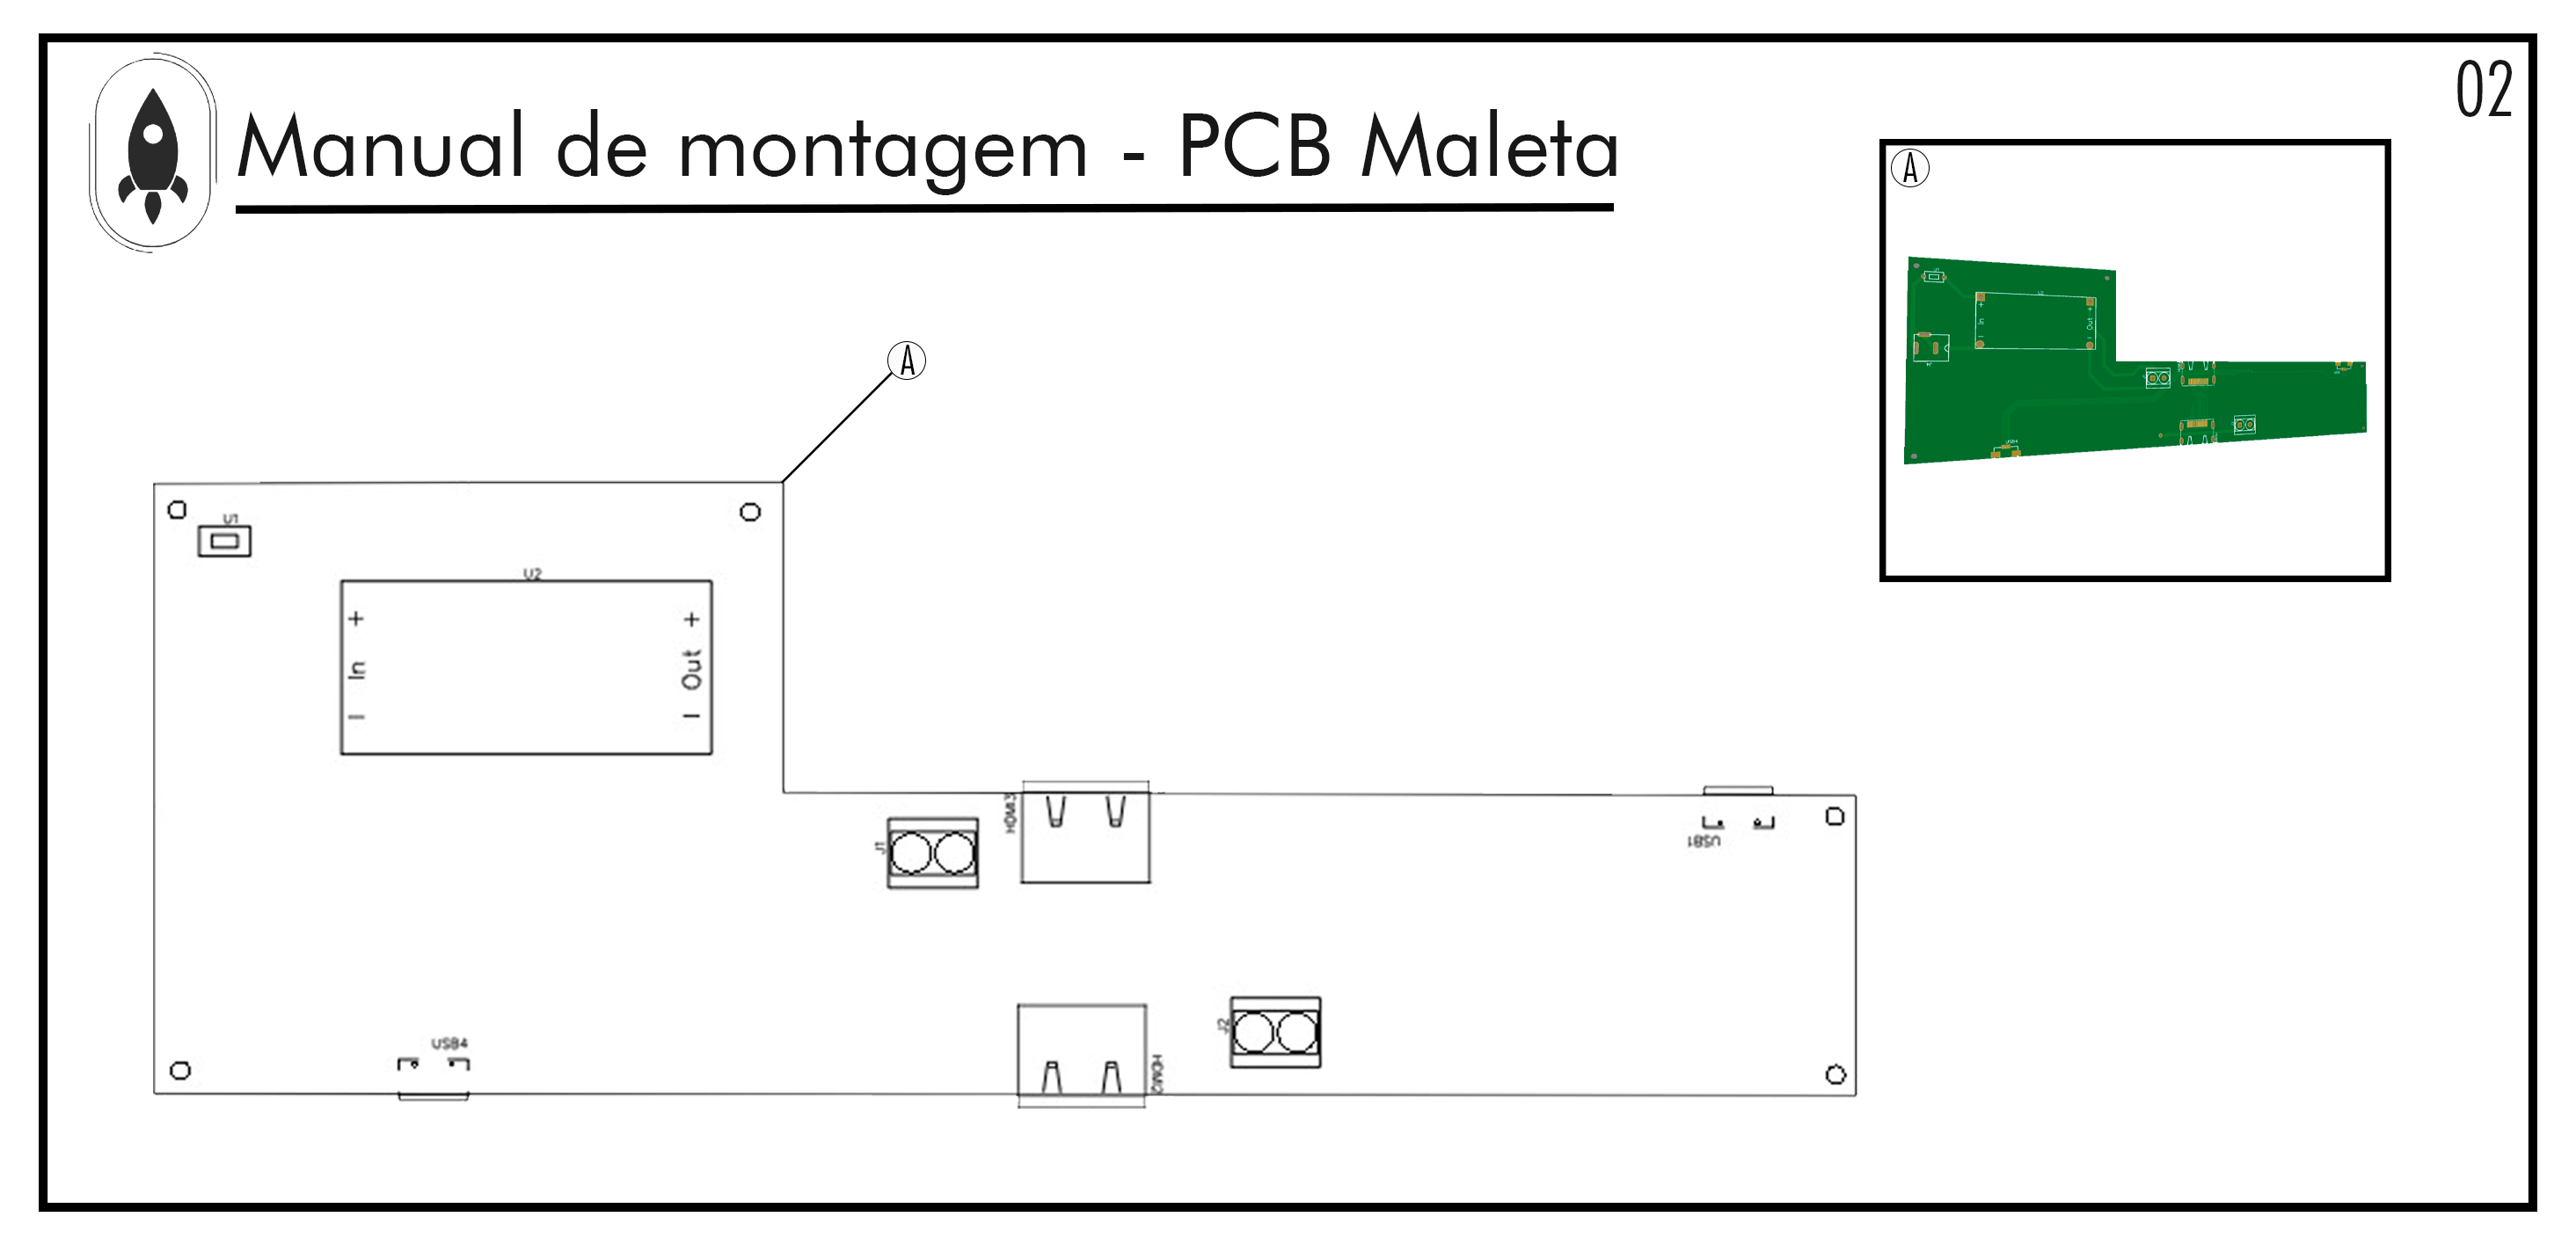
\includegraphics[width=\textwidth]{Figuras/MALETA/Pg-02---PL-01.png}
  \caption{PCI da maleta do usuário.}
 %{ \footnotesize Fonte: Autores} 
  \label{fig:Lista de materiasi MALETA}
\end{figure}
\newpage

\par Pegue o componente 'B'Conector Adaptador Plug P4 Macho com Borne ), encaixe-a na posição mostrada \ref{fig:PCBMALETA Jack} e solde junto a placa.
\begin{figure}[H]
  \centering
  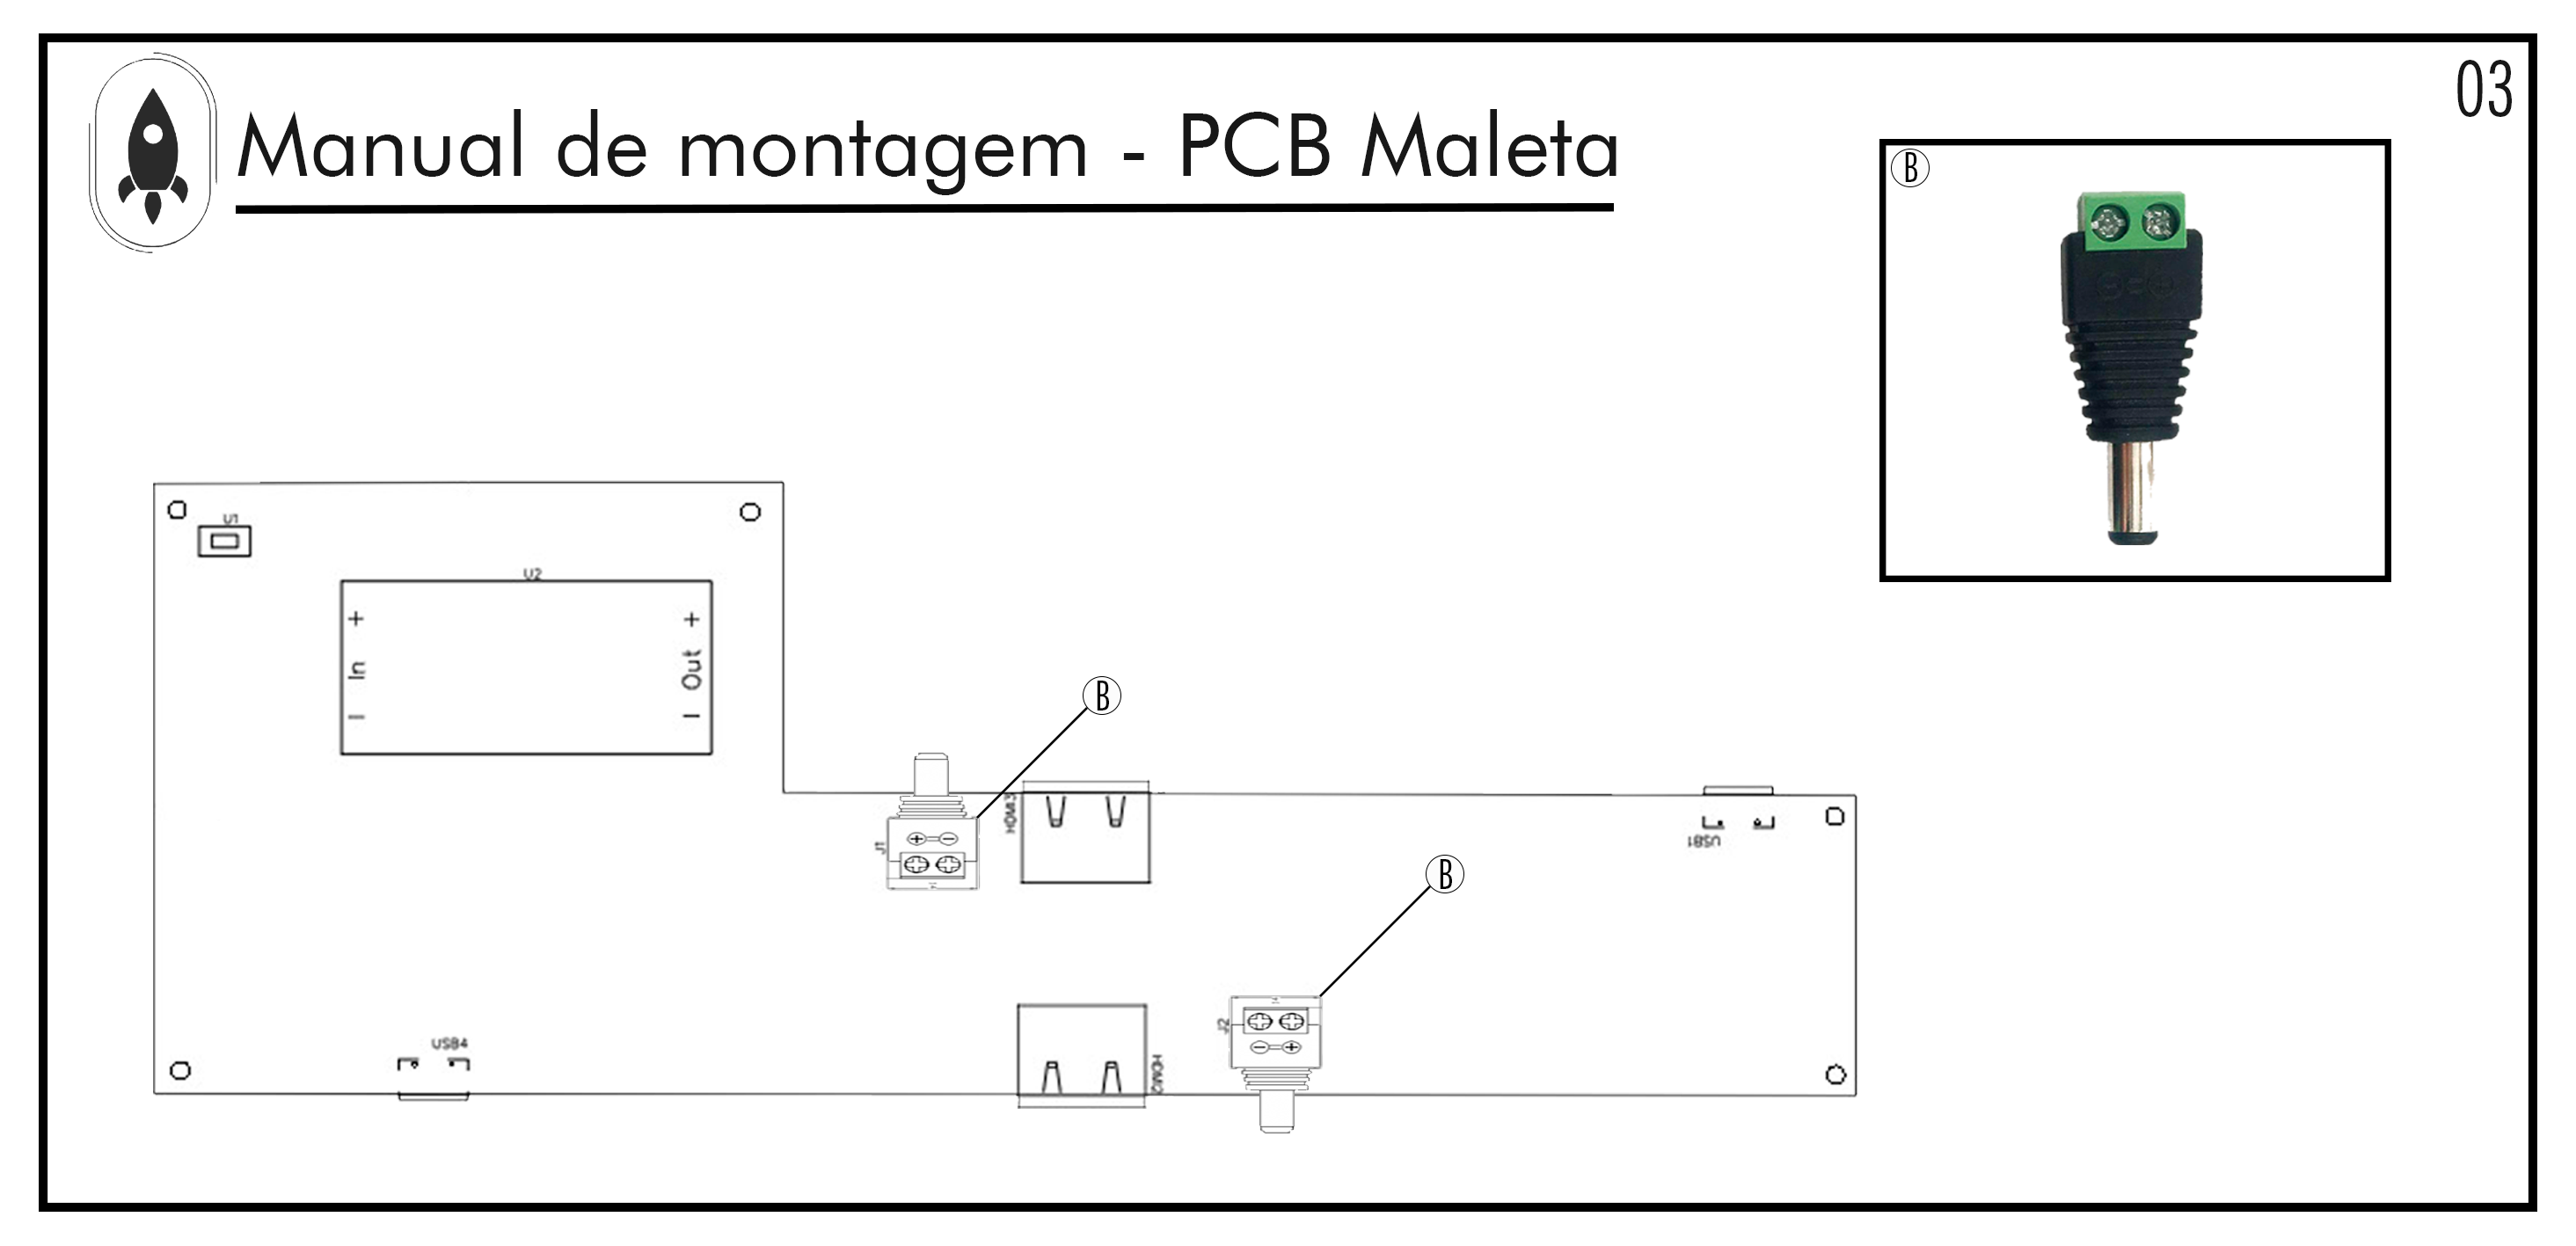
\includegraphics[width=\textwidth]{Figuras/MALETA/Pg-03---PL-01.png}
  \caption{Adaptador Jack DC macho.}
 %{ \footnotesize Fonte: Autores} 
  \label{fig:PCBMALETA Jack}
\end{figure}


\par Pegue o componente 'C'(Micro Usb V8 Macho), encaixe-a na posição mostrada \ref{fig:PCBMALETA Micro Usb} e solde junto a placa.

\begin{figure}[H]
  \centering
  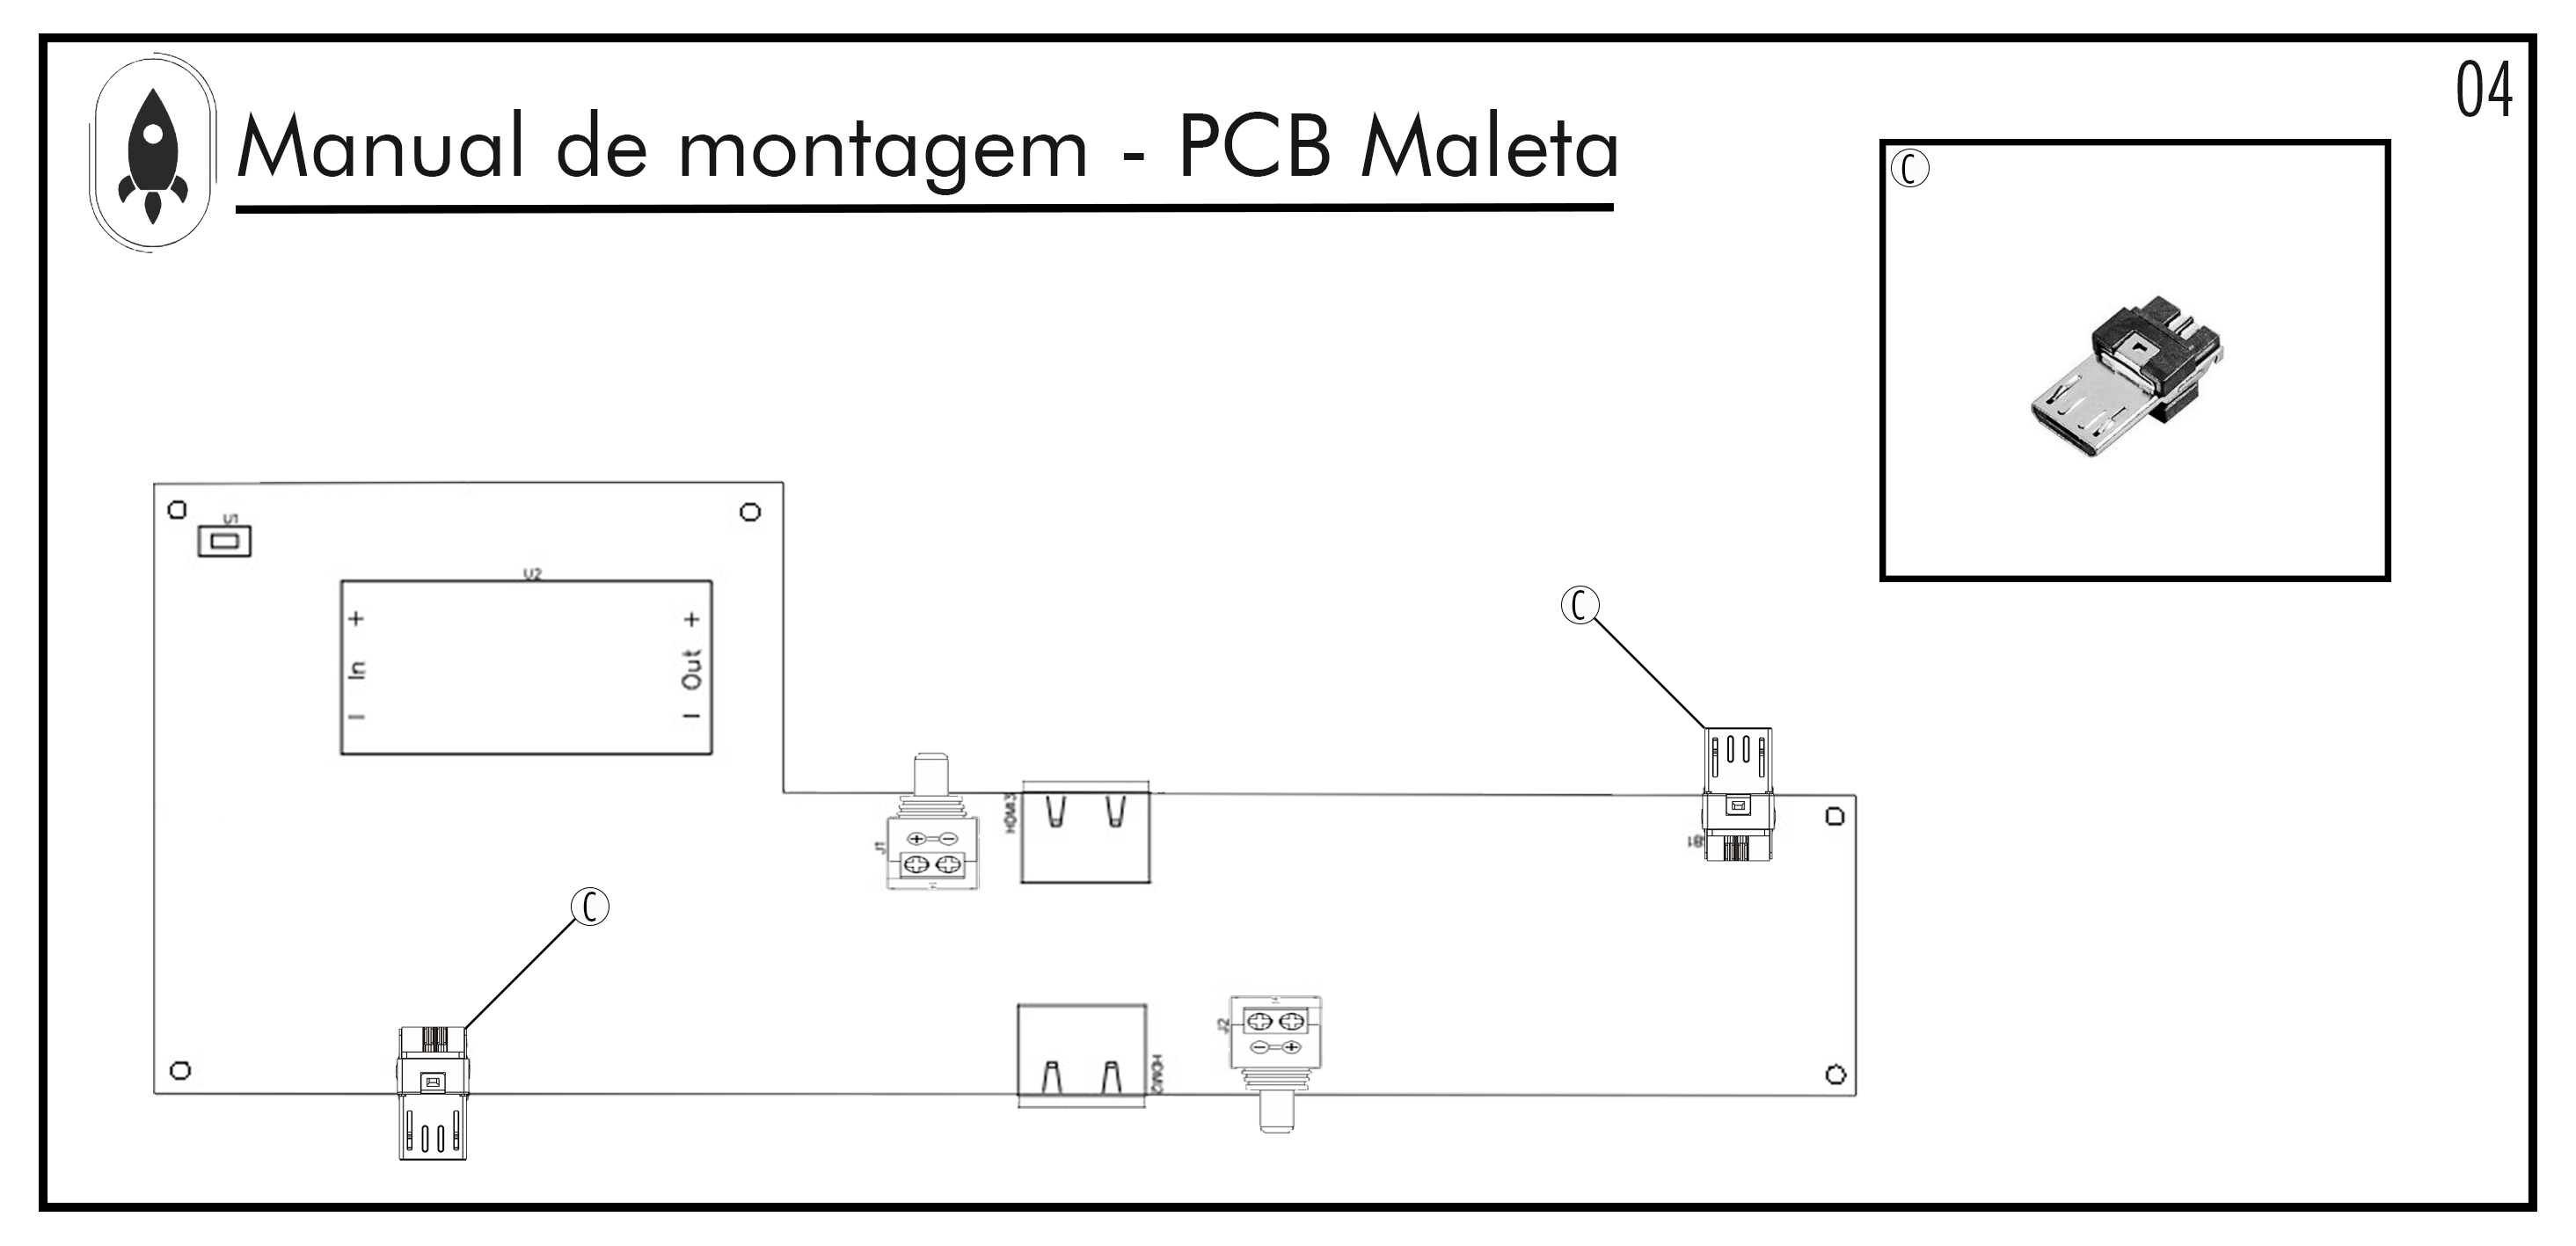
\includegraphics[width=\textwidth]{Figuras/MALETA/Pg-04---PL-01.png}
  \caption{Micro Usb V8 Macho.}
 %{ \footnotesize Fonte: Autores} 
  \label{fig:PCBMALETA Micro Usb}
\end{figure}

\newpage

\par Pegue o componente 'D'(Plug Hdmi Macho), encaixe-a na posição mostrada \ref{fig:PCBMALETA Hdmi} e solde junto a placa.
\begin{figure}[H]
  \centering
  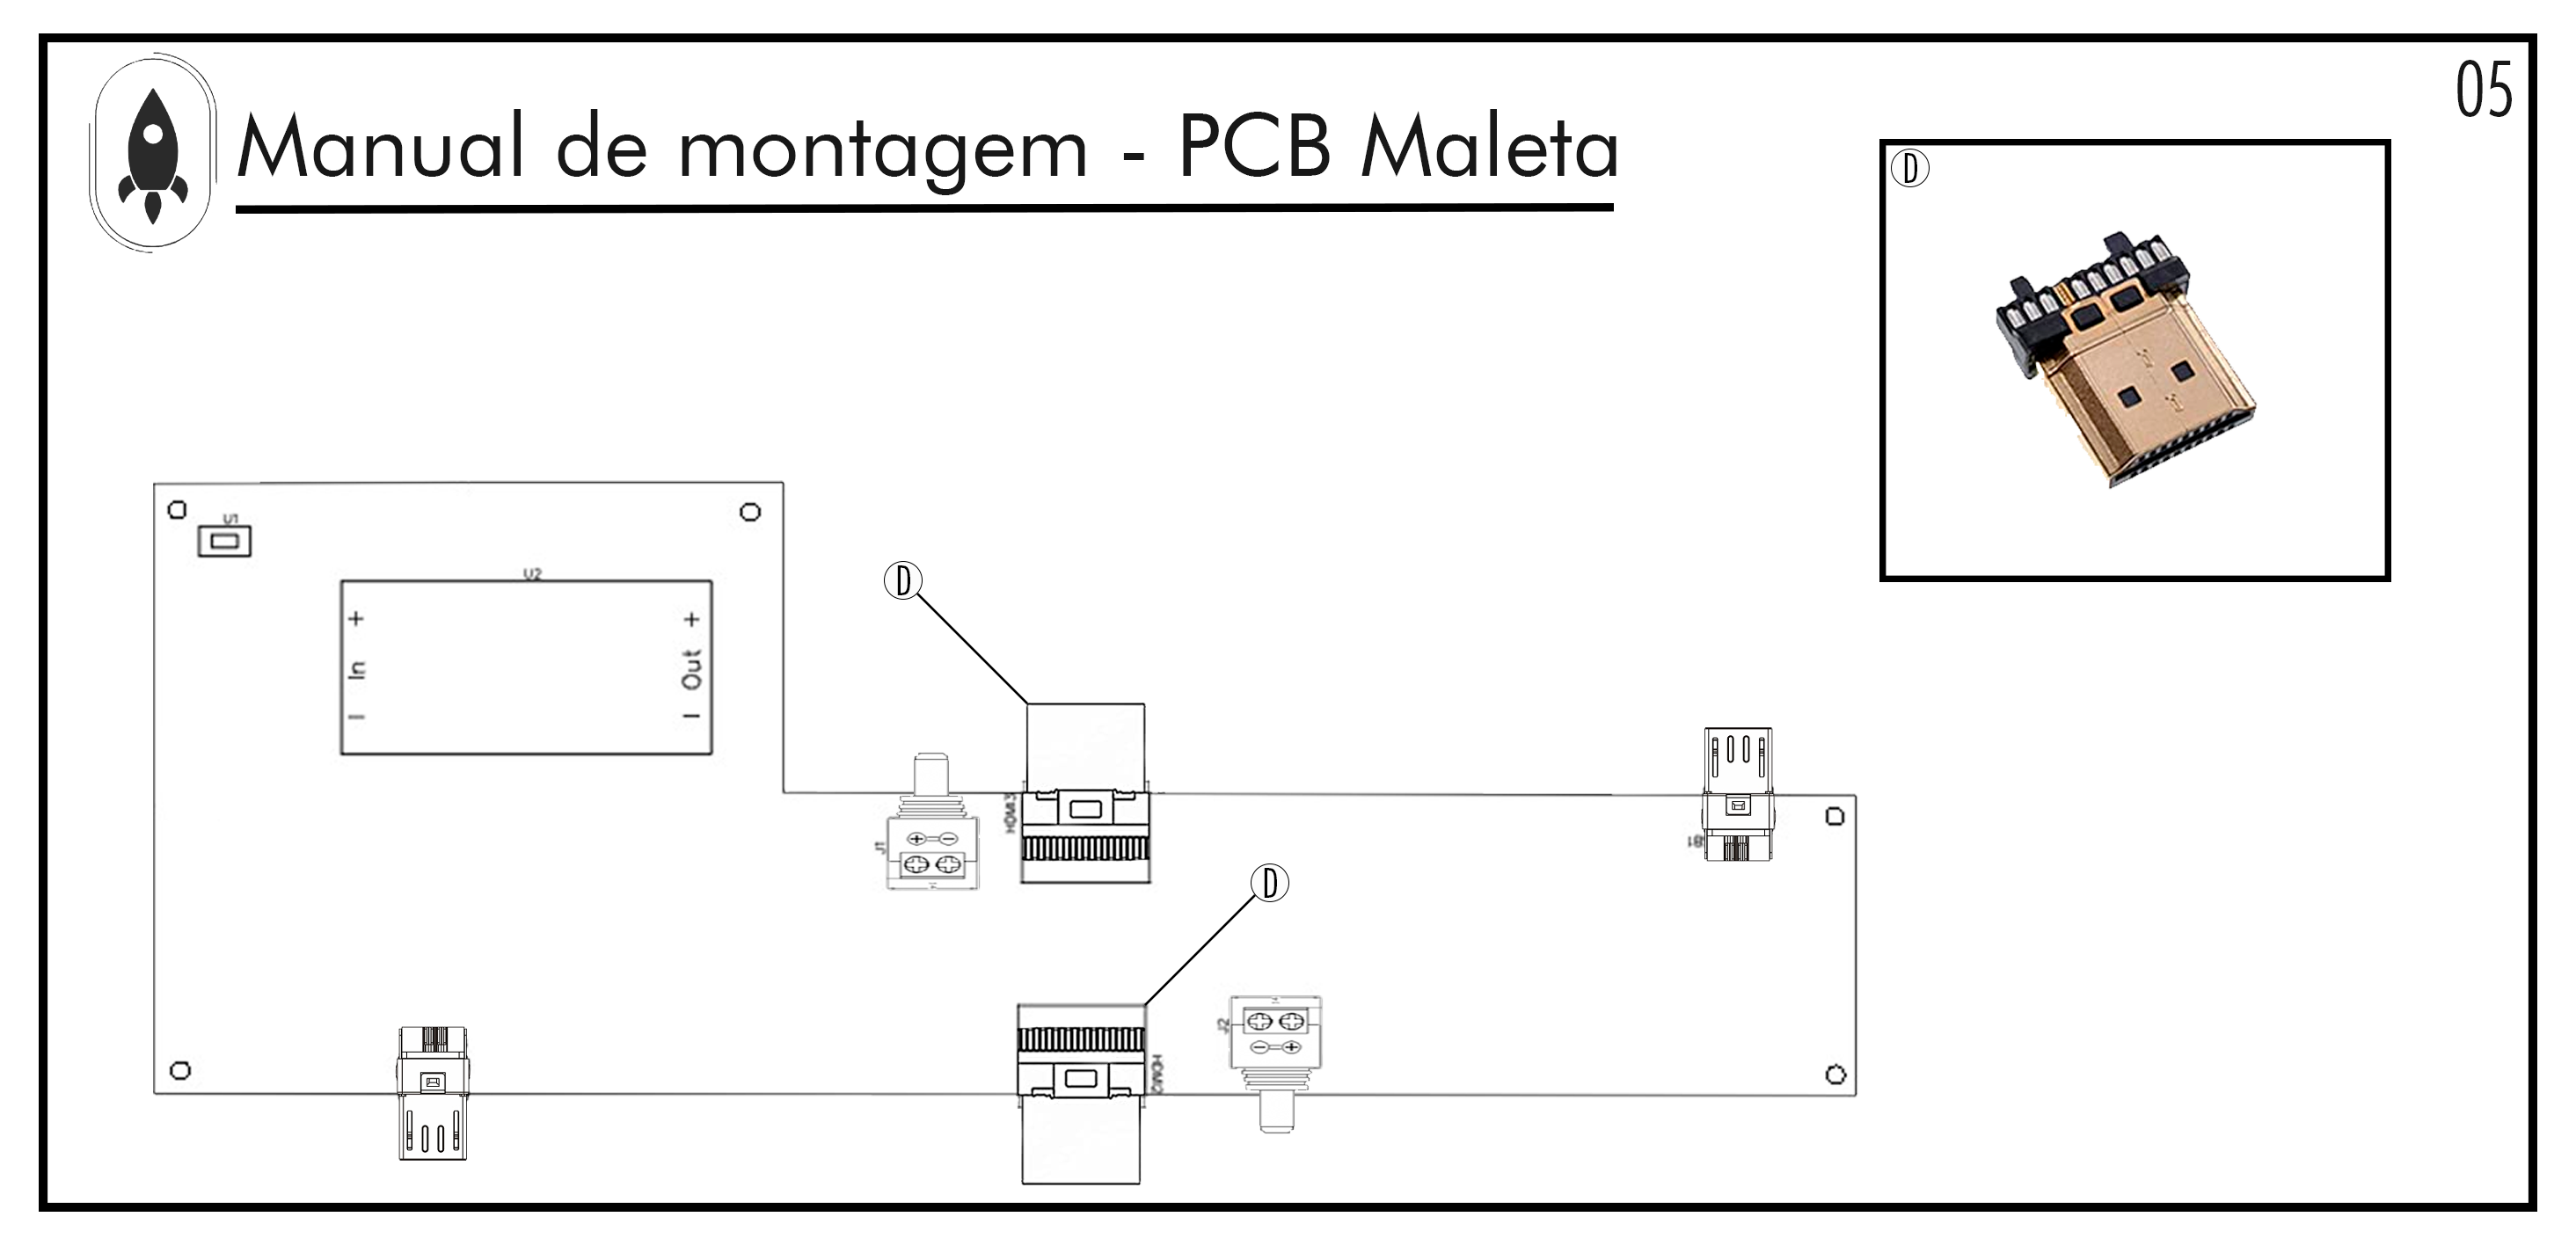
\includegraphics[width=\textwidth]{Figuras/MALETA/Pg-05---PL-01.png}
  \caption{Plug Hdmi Macho.}
 %{ \footnotesize Fonte: Autores} 
  \label{fig:PCBMALETA Hdmi}
\end{figure}


\par Pegue o componente 'E'(Conector fêmea Jack P4 2,5mm), encaixe-a na posição mostrada \ref{fig:PCBMALETA Jack} e solde junto a placa.

\begin{figure}[H]
  \centering
  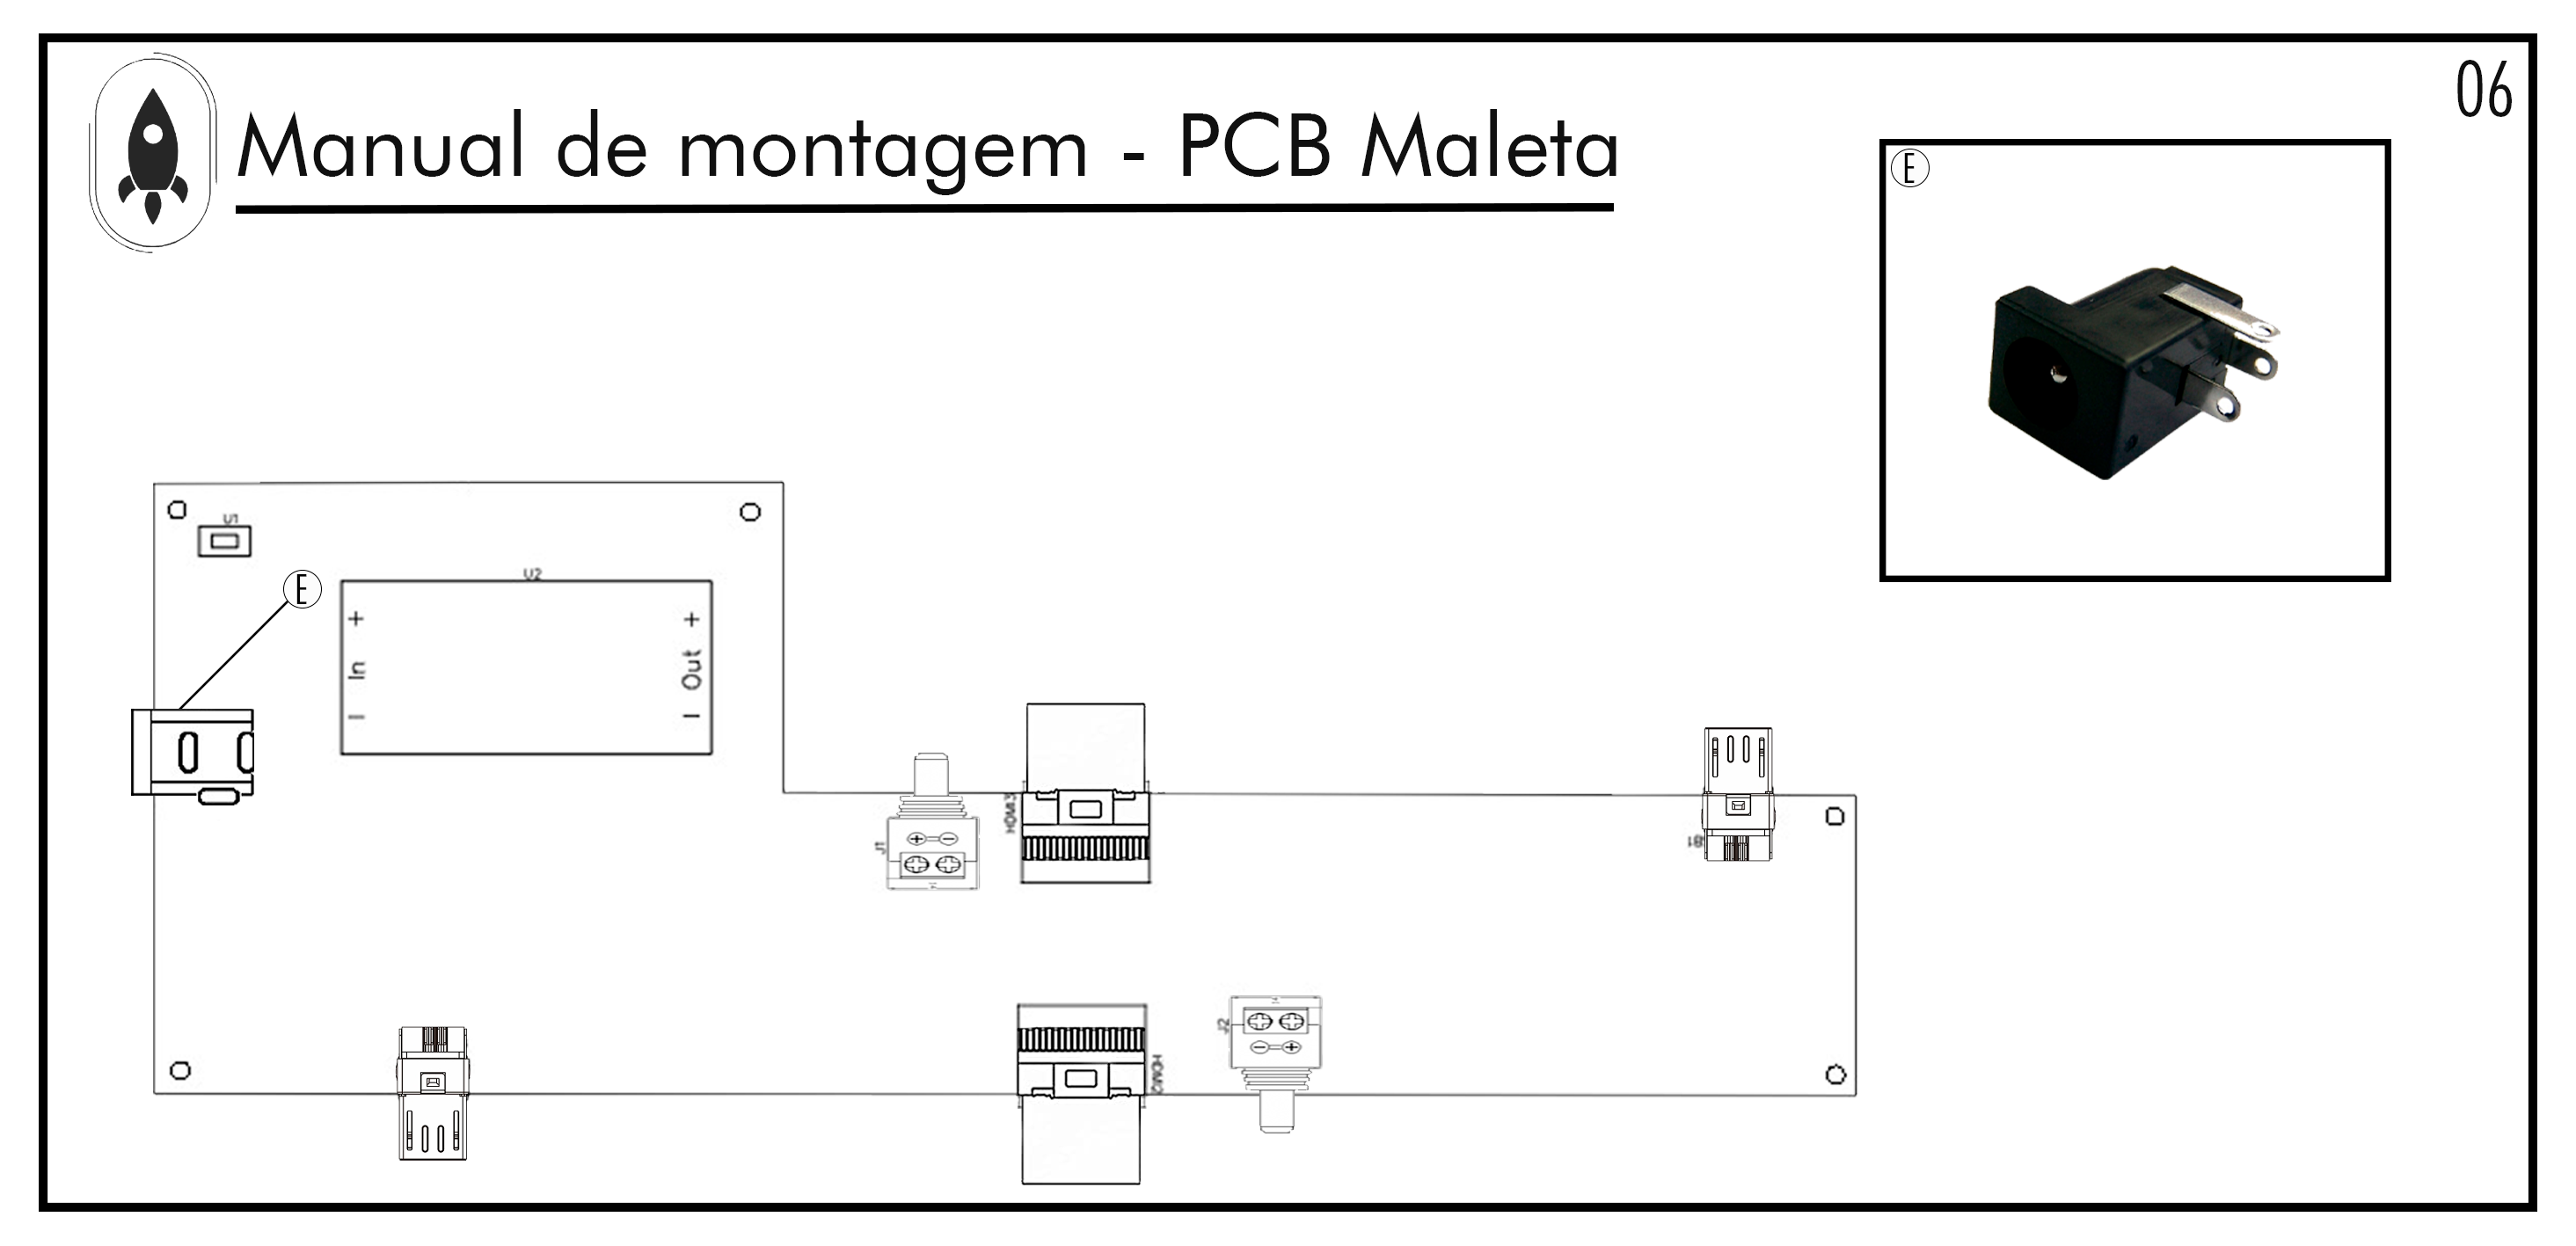
\includegraphics[width=\textwidth]{Figuras/MALETA/Pg-06---PL-01.png}
  \caption{Conector fêmea Jack P4 2,5mm.}
 %{ \footnotesize Fonte: Autores} 
  \label{fig:PCBMALETA Jack}
\end{figure}

\newpage

\par Pegue o componente 'F'(Chave Gangorra 2 Polos Mini), encaixe-a na posição mostrada \ref{fig:PCBMALETA CHAVE} e solde junto a placa.

\begin{figure}[H]
  \centering
  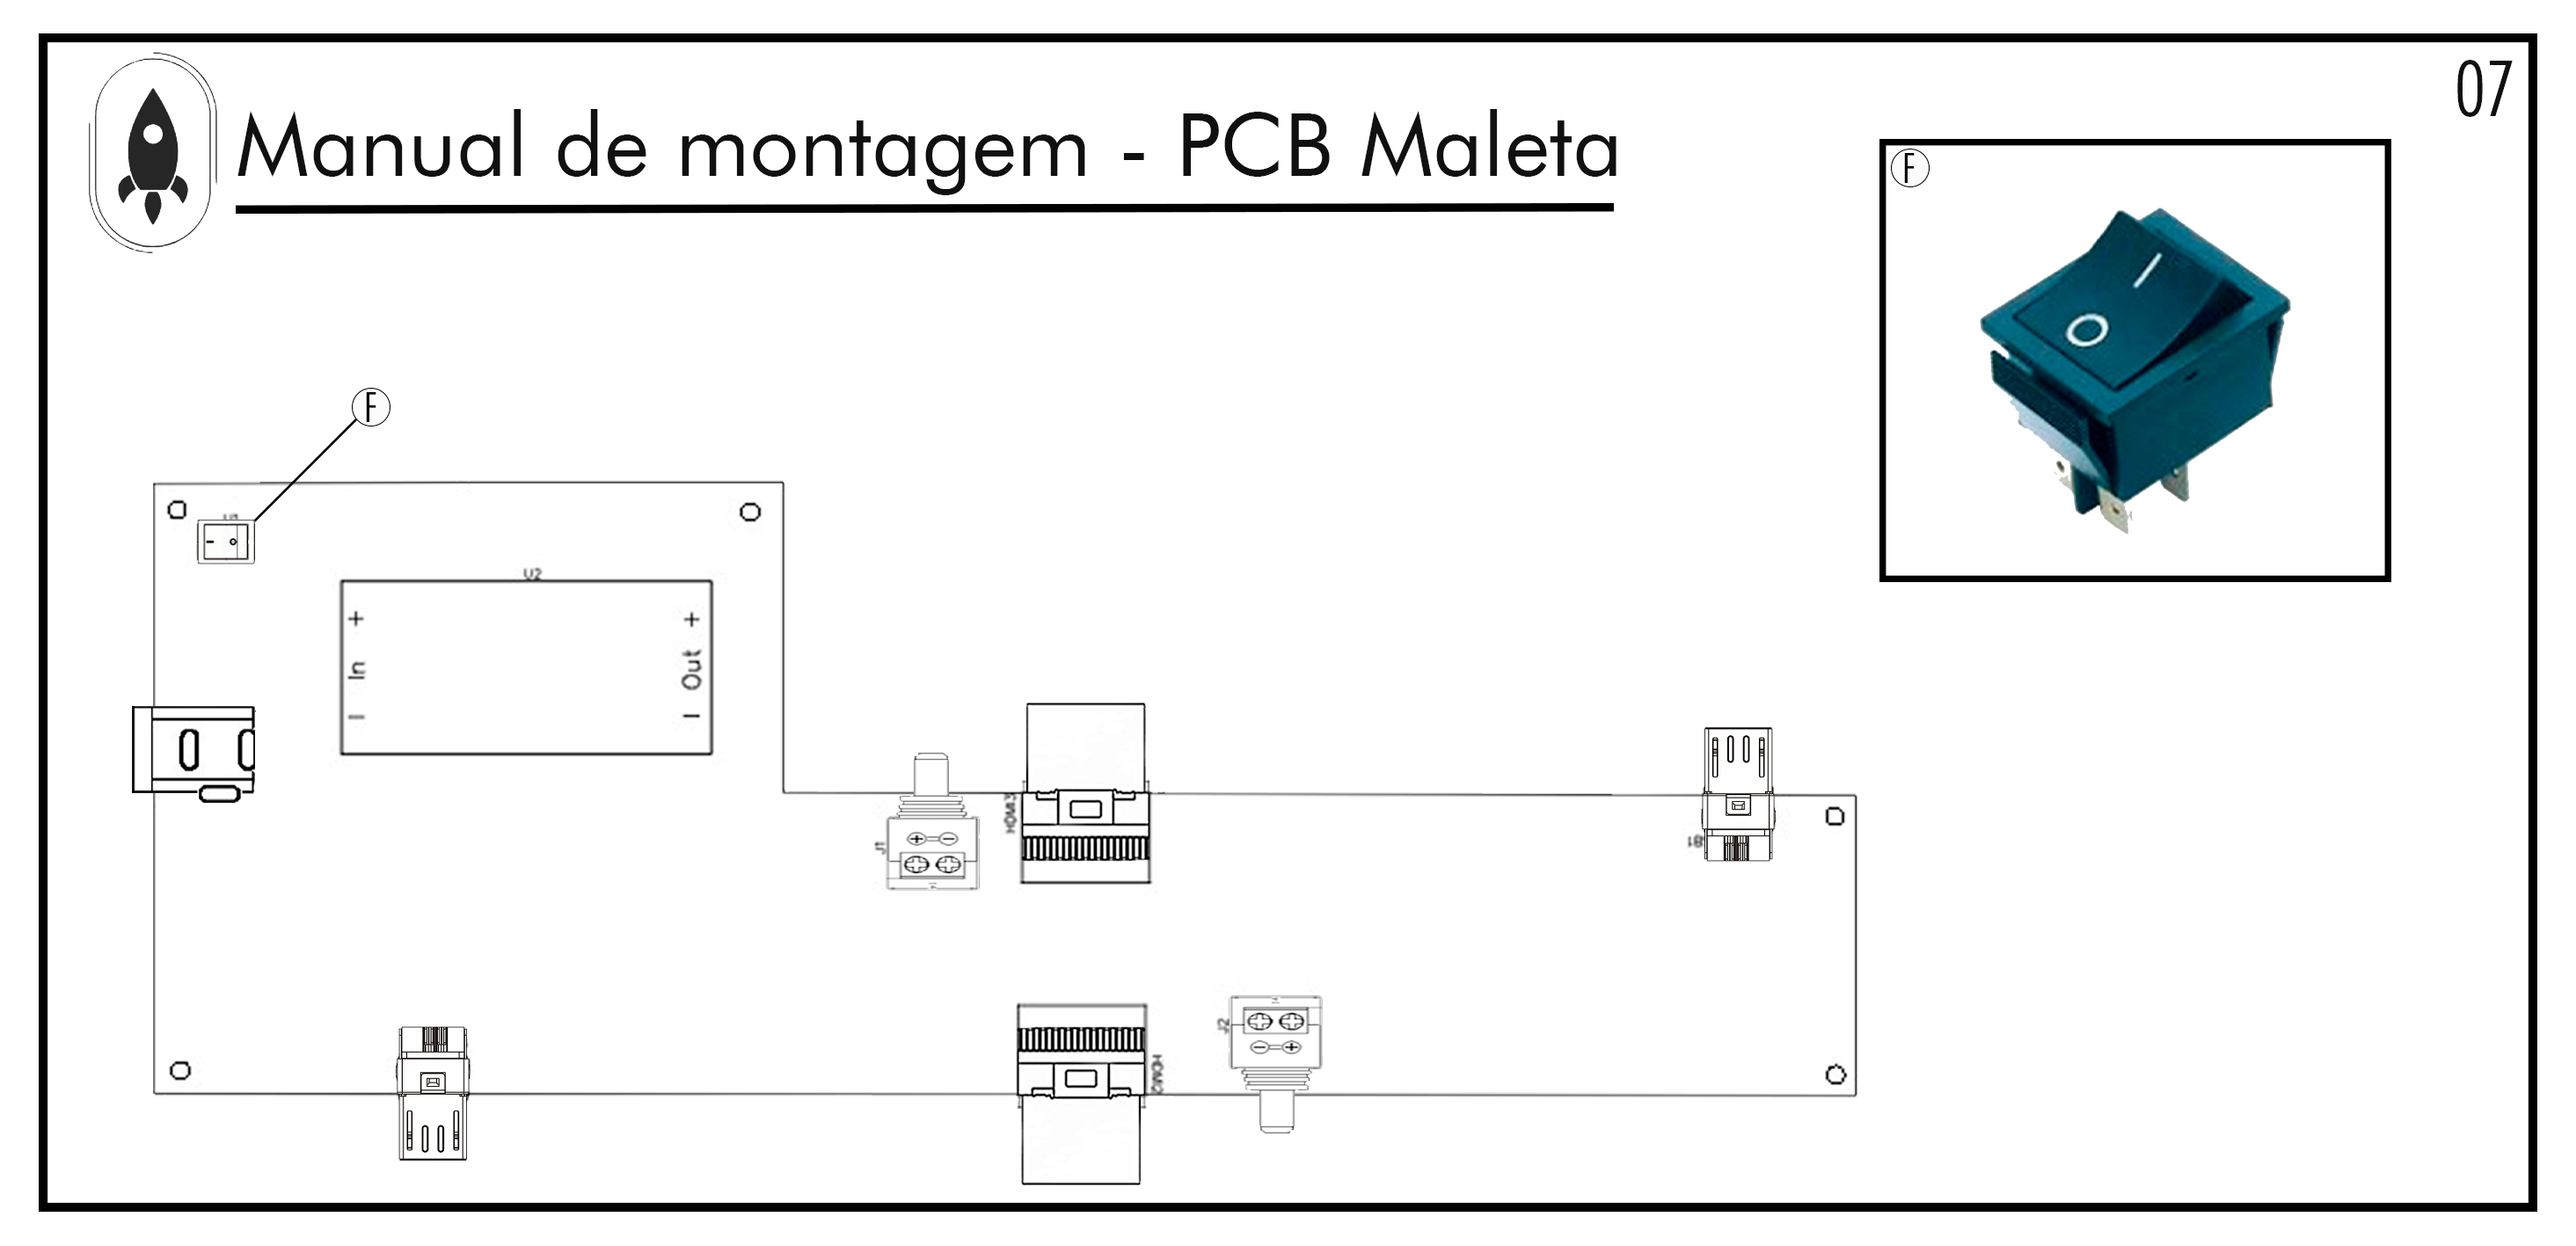
\includegraphics[width=\textwidth]{Figuras/MALETA/Pg-07---PL-01.png}
  \caption{Chave Gangorra 2 Polos Mini.}
 %{ \footnotesize Fonte: Autores} 
  \label{fig:PCBMALETA CHAVE}
\end{figure}

\par Pegue o componente 'G'(ESP32 LoRa WiFi), encaixe-a na posição mostrada \ref{fig:PCBMALETA LORA}

\begin{figure}[H]
  \centering
  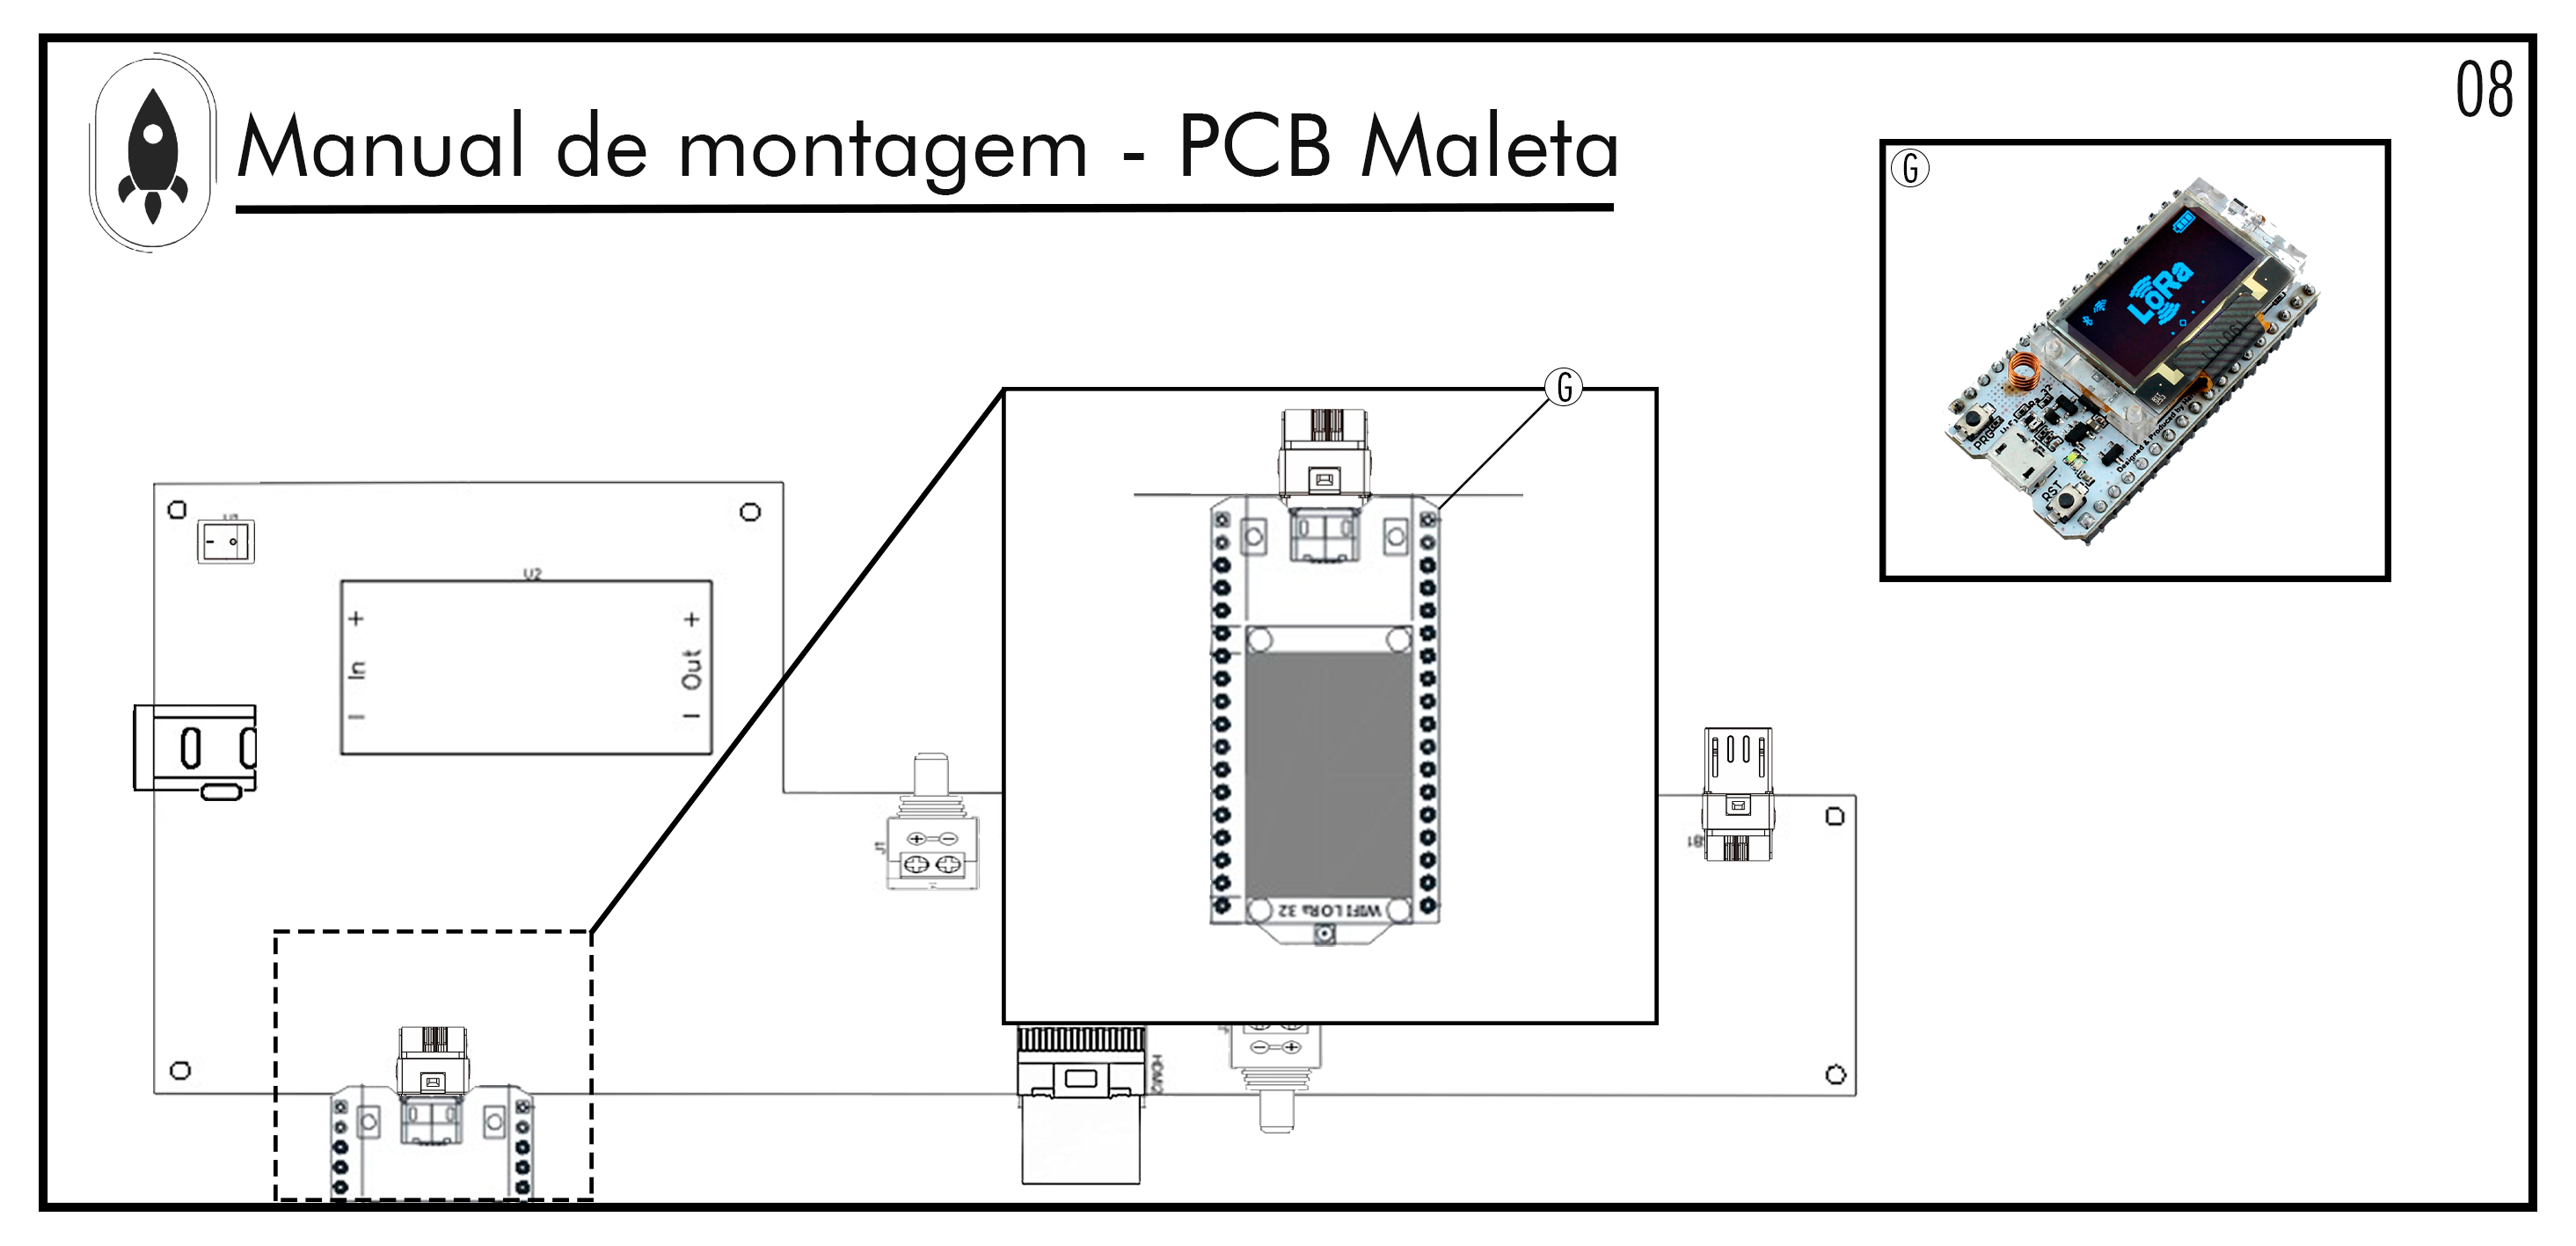
\includegraphics[width=\textwidth]{Figuras/MALETA/Pg-08---PL-01.png}
  \caption{ESP32 LoRa WiFi.}
 %{ \footnotesize Fonte: Autores} 
  \label{fig:PCBMALETA LORA}
\end{figure}
\newpage
\par Pegue o componente 'H'(NVIDIA Jetson Nano Developer Kit), encaixe-a na posição mostrada \ref{fig:PCBMALETA NVIDIA} 
\begin{figure}[H]
  \centering
  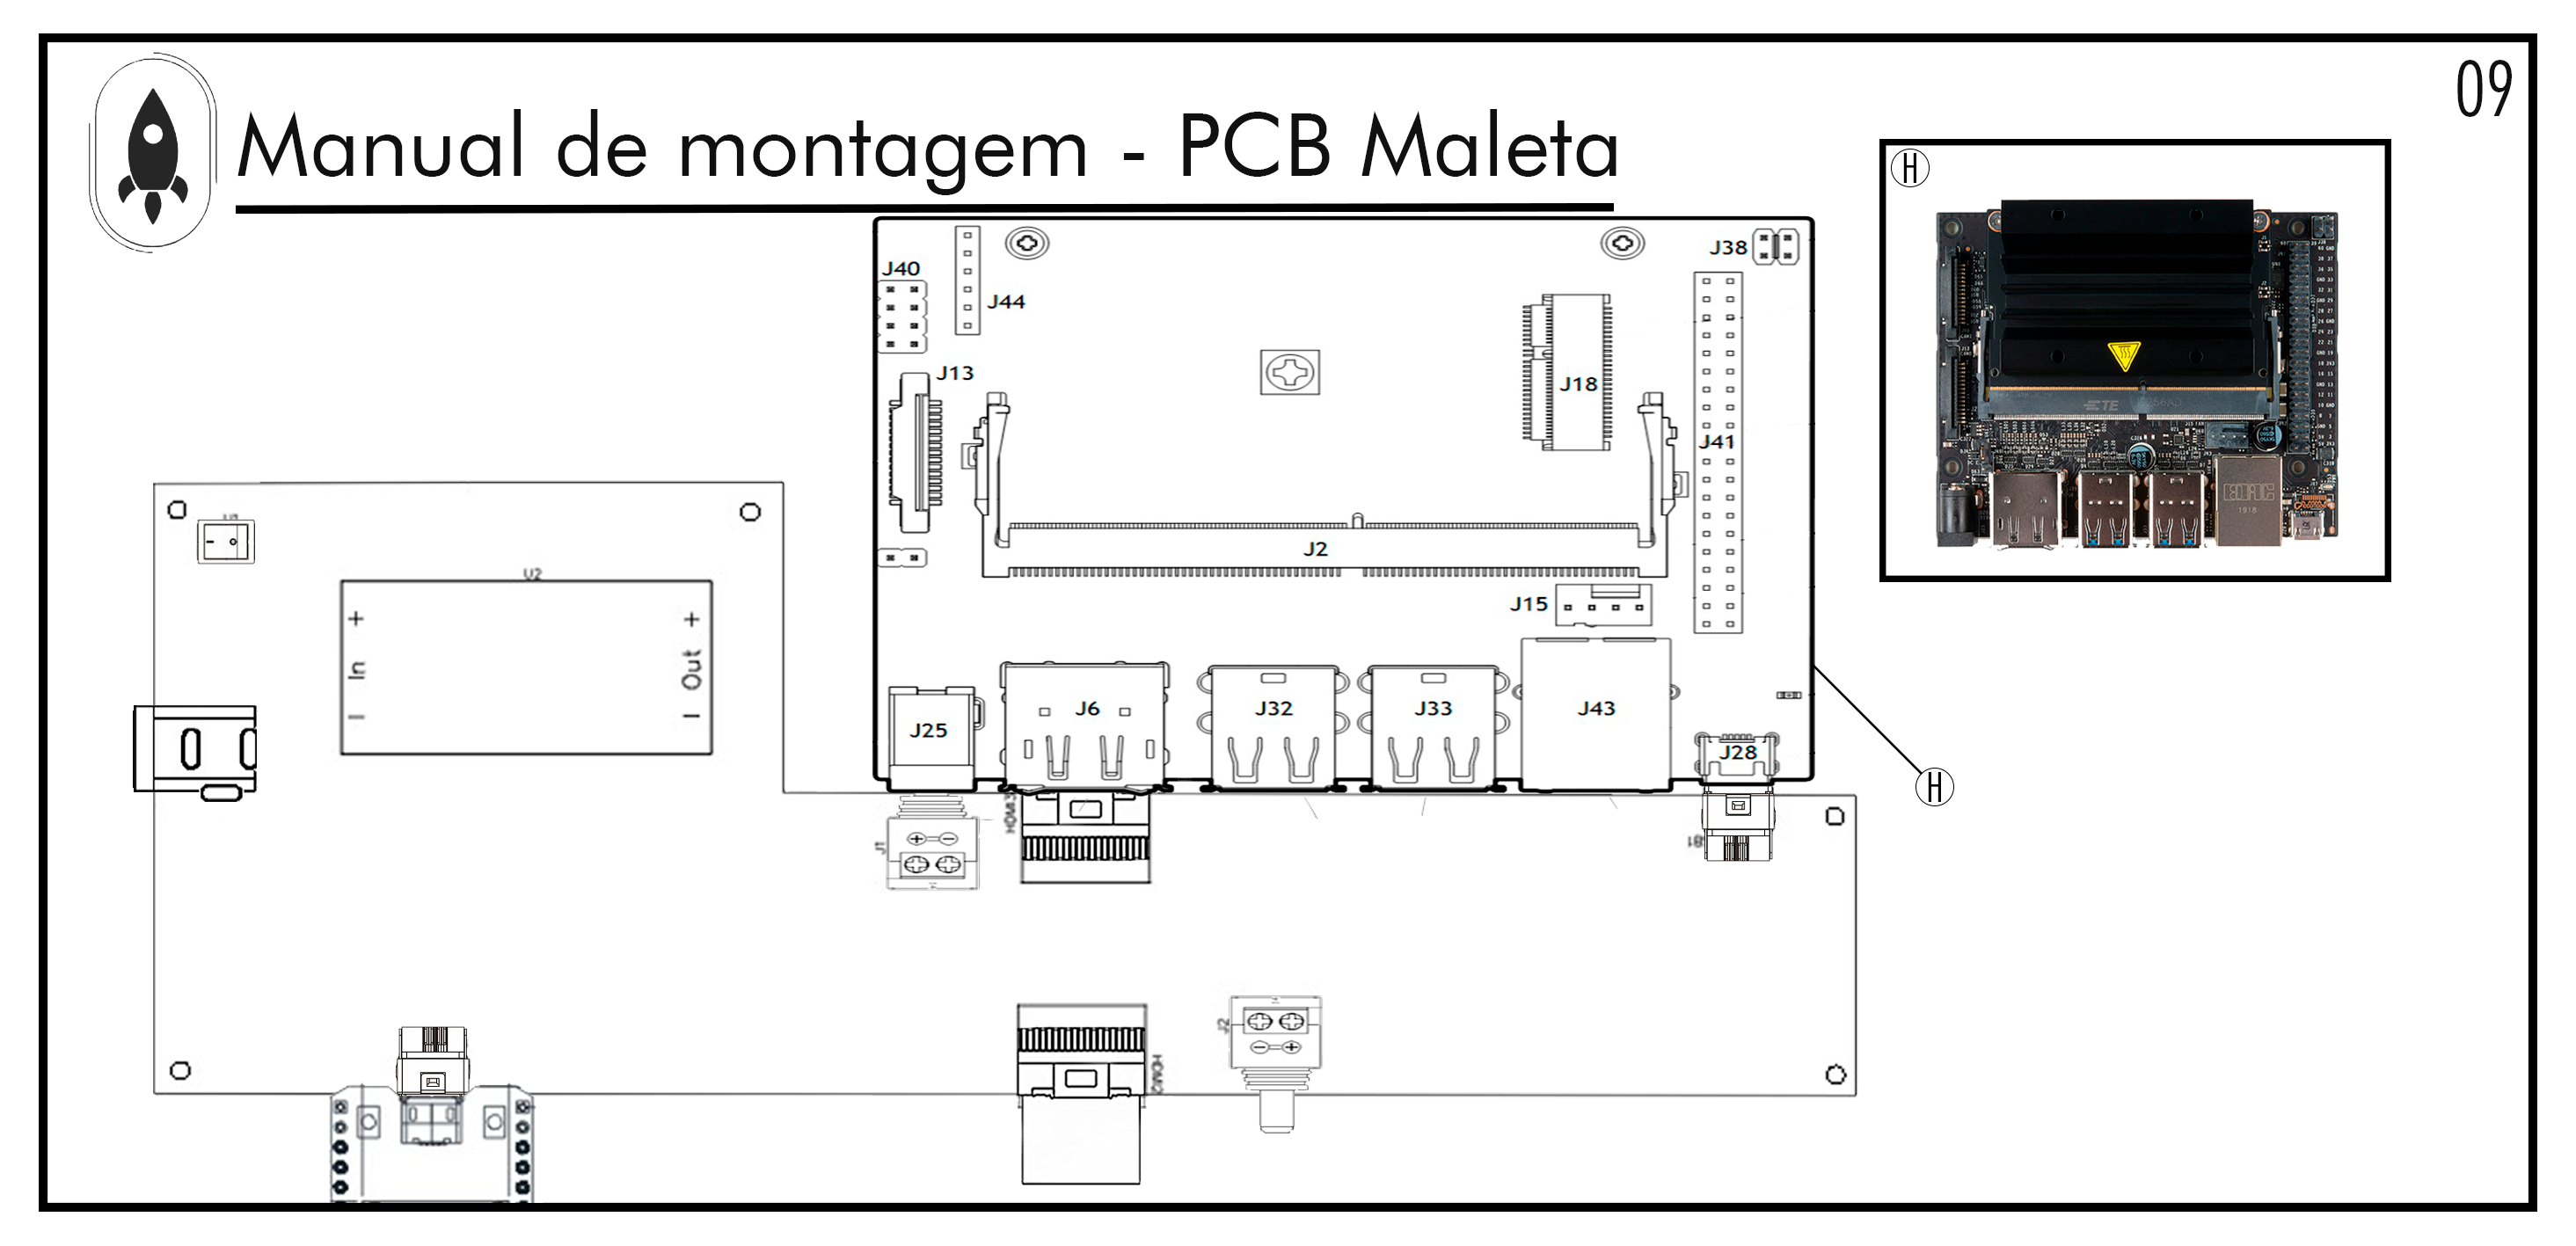
\includegraphics[width=\textwidth]{Figuras/MALETA/Pg-09---PL-01.png}
  \caption{NVIDIA Jetson Nano Developer Kit.}
 %{ \footnotesize Fonte: Autores} 
  \label{fig:PCBMALETA NVIDIA}
\end{figure}




\par Pegue o componente 'I'(Placa controladora PCB800099-V.9), encaixe-a na posição mostrada \ref{fig:PCBMALETA PCB800099} 

\begin{figure}[H]
  \centering
  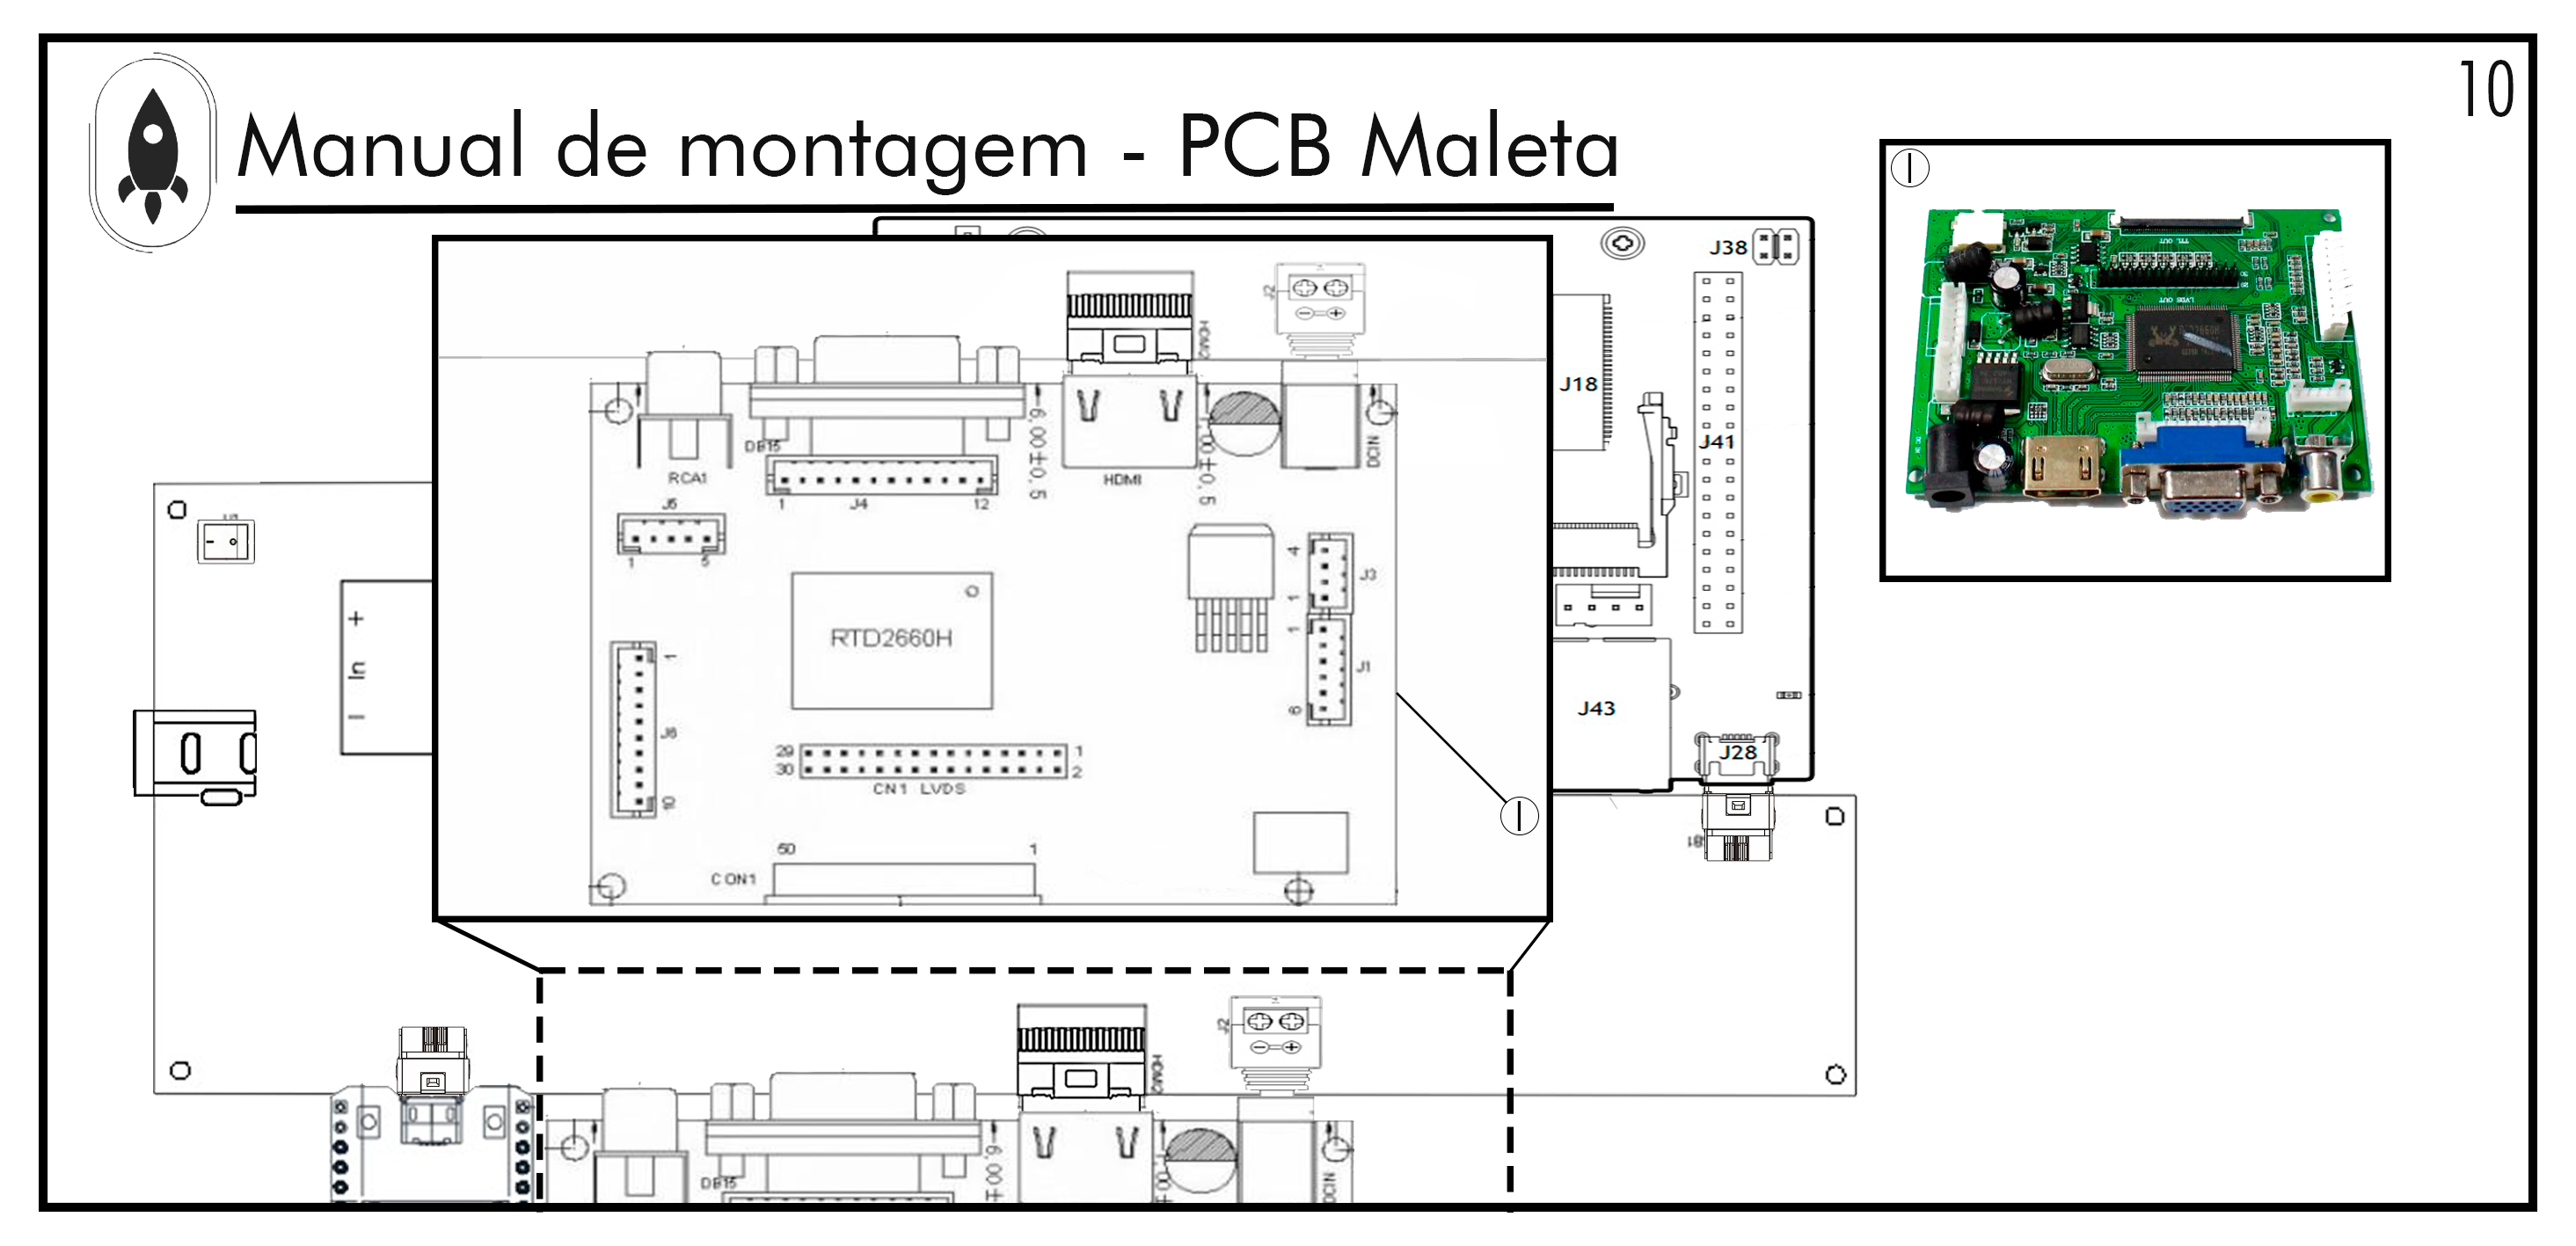
\includegraphics[width=\textwidth]{Figuras/MALETA/Pg-10---PL-01.png}
  \caption{Placa controladora PCB800099-V.9.}
 %{ \footnotesize Fonte: Autores} 
  \label{fig:PCBMALETA PCB800099}
\end{figure}

\newpage
\par Pegue o componente 'J'(LM2596), encaixe-a na posição mostrada \ref{fig:PCBMALETA LM2596} e solde junto a placa.
\begin{figure}[H]
  \centering
  \includegraphics[width=\textwidth]{Figuras/MALETA/Pg-11---PL-01.png}
  \caption{LM2596.}
 %{ \footnotesize Fonte: Autores} 
  \label{fig:PCBMALETA LM2596}
\end{figure}



\par Pegue o componente 'K'(Display LCD 9 polegadas), encaixe-a o cabo de 50 pinos na posição mostrada \ref{fig:PCBMALETA display}.

\begin{figure}[H]
  \centering
  \includegraphics[width=\textwidth]{Figuras/MALETA/Pg-12---PL-01.png}
  \caption{Display LCD 9 polegadas.}
 %{ \footnotesize Fonte: Autores} 
  \label{fig:PCBMALETA display}
\end{figure}
\newpage
\par Pegue o componente 'L'(Mini Teclado slim com Touchpad), encaixe-a na posição mostrada \ref{fig:PCBMALETA Teclado} através de um cabo usb.
\begin{figure}[H]
  \centering
  \includegraphics[width=\textwidth]{Figuras/MALETA/Pg-13---PL-01.png}
  \caption{Mini Teclado slim com Touchpad.}
 %{ \footnotesize Fonte: Autores} 
  \label{fig:PCBMALETA Teclado}
\end{figure}


\subsection{Fixação das PCI's} \label{sec:fixação  }
\par Para a correta fixação das placas de circuito impresso nos seus respectivos lugares é necessário a utilização dos parafusos e porcas extensoras de modo a garantir a fixação adequada e a integridade dos componentes.
\begin{itemize}
    \item 1-Pegue a porca extensora, posicione-a sobre o local do parafuso,
     \item 2-Pegue a placa, posicione-a sobre o porca extensora,
     \item 3-Pegue o parafuso, posicione-a sobre o local de colocar o parafuso da placa,
    \item 4-Com ajuda de uma chave philips parafuse-o sem apertar de mais para evitar problemas mecânicos a placa,
    \item 5-Repita o processo para outros parafusos.
     
\end{itemize}

\begin{figure}[H]
  \centering
  \includegraphics[scale=0.1]{Figuras/100pcs-lot-10-brass-standoffs-m3-hex-nut.jpg}
    \includegraphics[scale=0.3]{Figuras/parafuso.png}
  \caption{Parafuso e porca extensora M5.}
  \label{fig:parafusos}
\end{figure}

\subsection{Case de proteção PCI's da Base de Lançamento}
\par Para acomodar e proteger a placa responsável pelo hardware na base de lançamento foi feita uma case de proteção conforme mostrada na figura \ref{fig:Case de proteção da PCI vistas} nela sera acomodada a PCI e alguns conectores para organizar as saídas.
\begin{figure}[H]
  \centering
  \includegraphics[scale=0.4]{Figuras/BASE/case f.png}

  \caption{Case de proteção da PCI saídas.}
  \label{fig:Case de proteção da PCI saídas}
\end{figure}
\begin{figure}[H]
  \centering
 % \includegraphics[scale=0.7]{Figuras/BASE/case iso.png}
  \includegraphics[scale=0.5]{Figuras/BASE/Sem título.png}
    \includegraphics[scale=0.7]{Figuras/BASE/case.png}
  \caption{Case de proteção da PCI vistas.}
  \label{fig:Case de proteção da PCI vistas}
\end{figure}
\PAR Os fios que alimentaram os motores e as células de cargas vão sair dos reles acoplados na PCI para conectores P4 acoplados a case de proteção para facilitar o encaixe dos fios até os atuadores como mostrado na figura \ref{fig:Case de proteção da PCI render}, são cabos Antichama Flexível 450/750 V de seção nominal 0,75mm².

\begin{figure}[H]
  \centering
  \includegraphics[scale=0.2]{Figuras/BASE/untitled.11.jpg}
  \includegraphics[scale=0.2]{Figuras/BASE/untitled.12.jpg}
  \caption{Case de proteção da PCI.}
  \label{fig:Case de proteção da PCI render}
\end{figure}
\chapter{Sistema de carregamento}

\section{Lista de materiais}

\begin{table}[H]
\centering
\begin{tabular}{|m{1.8cm} |m{8.8cm}|m{3.5cm}|}
\hline
\begin{center}Quantidade\end{center} & \begin{center}Componente\end{center} &\begin{center} Part Number\end{center} \\\hline

 01&Cabo de Força (1,5m) lec 320 C13 - Fêmea Flexível Tripolar 3x0,75$mm^2$ & lec 320 C13 \\\hline
 
01 &  Tomada de força lec 320 C14 - Macho
& lec 320 C14 \\\hline
  
01& Chave seletora de tensão HH 127/220V  & Chave HH \\\hline
   
01& Transformador 110/220V para 30V 1A & Transformador \\\hline

01&Cabo PP 2x2.5$mm^2$ (1m) & Cabo PP \\\hline

02&Plug Conector Jack J4  Macho & Jack Macho \\\hline

01& Conector Jack J4 DC-015 Fêmea 2.1$mm^2$ &Jack Fêmea \\\hline

01& Capacitor - 1000uF/50V & - \\\hline

02& Diodos 1N4007V & 1N4007  \\\hline

01& Transistor NPN BC547 & BC547\\\hline

01& Regulador de tensão L7812 & L7812 \\\hline

01& Regulador de tensão LM317 &  LM317 \\\hline

01& Resistor 240R - 1/4W & - \\\hline

01& Resistor 1KR  - 1/4W & - \\\hline

01& Resistor 0.12R - 1/4W & - \\\hline

05 & Terminal Faston Fêmea &   DJ623-A6  \\\hline

01 & Metro - Cabo flexível 2,5 mm² Verde & - \\\hline

\end{tabular}
\caption{Lista de componentes}
\end{table}

\section{Ferramentas}

\par Para a soldagem dos componentes eletrônicos na PCI (Placas de Circuito Impresso), conexões dos fios com os dispositivos e fixação da PCI na case de proteção ou outro local, é necessário o uso das seguintes ferramentas e acessórios:

\begin{itemize}
    \item Ferro de Solda ou Estação de Solda (15W-40W)
    \item Solda Estanho em fio 1mm
    \item Esponja metálica ou esponja convencional para limpeza da ponta de solda
    \item Lupa com suporte e pinça, para apoio e manuseio da PCI
    \item Sugador de solda
    \item Chave de fenda/phillips
    \item Alicate de corte pequeno
    \item Alicate de desencapar ou estilete
    \item Multímetro
\end{itemize}

\begin{center}
ATENÇÃO
\begin{figure}[H]
 \centering
 \includegraphics[scale = 0.1]{Figuras/atenção.png}
\end{figure}
\end{center}

\par Os ferros de solda aquecem a temperaturas superiores a 400ºC. Usar um suporte para ferro de solda decente é fundamental para não se acidentar e sofrer com queimaduras. Além disso, certifique-se de trabalhar em uma área bem ventilada ou use um extrator de fumaça ou exaustor de fumaça. Os vapores do fluxo são tóxicos. Leia atentamente as instruções deste manual. Ao soldar, utilize Equipamentos de Proteção Individual (EPIs), tais como, óculos de segurança e luvas de segurança. Mantenha todo o cabelo, roupas folgadas e joias protegidos e fora do caminho de suas ferramentas. Se a solda que você estiver usando contiver chumbo, lave as mãos após concluir o trabalho.


\subsection{Boas práticas}
\PAR É de bom grado ter alguns cuidados ao montar e manter em boas condições as placas de circuito impresso-PCI que estão sujeito a vários fatores de risco como:
\begin{itemize}
\item \textbf{Mecânicos:}
\begin{itemize}
\item Vibrações
\item flexões nas PCI 
\item choques mecânicos
\end{itemize}
\end{itemize}

\begin{itemize}
\item \textbf{Ambientais:}
\begin{itemize}
\item Umidade em excesso
\item Contaminantes pelo ar 
\item Excesso de luz solar
\end{itemize}
\end{itemize}

\begin{itemize}
\item \textbf{Eletrostático:}
\begin{itemize}
\item Descargas elétricas produzidas por atrito e contato humano sem devidos cuidados
\end{itemize}
\end{itemize}

\par {\textbf{Alguns cuidados devem ser tomados:}}

\begin{itemize}
\item Evitar tocar em partes metálicas dos componentes e nos conectores e minimizar o manuseio o máximo possível evitando danos mecânicos;
\item É recomendável segurar a placa de forma a não tocar nas suas trilhas preferível que o manuseamento da mesma seja feito de forma que a pessoa segura a placa pelas suas bordas/ laterais;  

\item Nunca flexione a placa ou utilize de muita força ao manuseá-la pode acarretar em rompimento das trilhas,rompimentos de ligações  de encaixe;

\item Não deixe os equipamentos perto de recipientes com água e nem molhe-os.
\end{itemize}

\section{Impressão da PCI do Carregador}

\par Para a confecção da placa de circuito impresso foi gerado o arquivo Gerber de cada placa de circuito impresso, sendo gerado um arquivo em formato ZIP disponível em Arquivos Gerber sendo fabricadas com 2 Layers com a placa contendo uma espessura de $1.6 mm$ e peso de cobre de $1 oz$. Para a visualização dos arquivos Gerber é necessário a utilização de um programa de prototipagem de placas de circuito impresso ou um visualizador desse tipo de arquivo disponível para download no site do programa utilizado para o projeto EasyEda como pode se observado na figura \ref{fig:Gerber}. A placa de circuito impresso que será confeccionada é apresentada na figura \ref{trilha-carregador}.

\par Link download arquivos Gerber: \href {https://drive.google.com/drive/folders/1P1pQGE_zuSLOB5qd8zfESWqLDwtyoRKd?usp=sharing}{aqui}
\par Link download do programa vizualizador: \href{https://sourceforge.net/projects/gerbv/files/}{aqui} 

\begin{figure}[H]
  \centering
  \includegraphics[width=\textwidth]{Figuras/Carregador/PCB_PCB_2020-11-10_21-13-48_2020-11-20_03-04-03.png}
  \caption{Trilhas PCI - Carregador.} 
 %{ \footnotesize Fonte: Autores} 
  \label{trilha-carregador}
\end{figure}

\newpage

\section{Instruções de Montagem do Carregador}

\par A montagem correta da placa é de suma importância para o correto funcionamento do carregador das baterias do projeto, siga os passos a seguir para garantir a correta montagem da placas de circuito impresso e a conexão dos dispositivos da fonte de carregamento.

\begin{figure}[H]
  \centering
  \includegraphics[scale = 0.15]{Figuras/atenção.png}
\end{figure}


\subsection{PCI do Carregador}
%\subsection{Materiais}
\par Primeiramente é necessário ter em mão todos os componentes para sua montagem \ref{carregador01}.

\begin{figure}[H]
  \centering
  \includegraphics[width=\textwidth]{Figuras/Carregador/carregador_manual_01.jpg}
  \caption{Lista de Materiais - Fonte de Carregamento.} 
 %{ \footnotesize Fonte: Autores} 
  \label{carregador01}
\end{figure}

Com todos os componentes em mãos, pegue componente 'A’(Capacitor - 1000uF/50V), encaixe no local indicado na figura \ref{carregador02} e solde o componente na PCI passando uma fina camada de solda nos terminais e com o uso do alicate cuidadosamente corte as sobras de seus terminais.

\begin{figure}[H]
  \centering
  \includegraphics[width=\textwidth]{Figuras/Carregador/carregador_manual_02.jpg}
  \caption{Capacitor - 1000uF/50V.} 
 %{ \footnotesize Fonte: Autores} 
  \label{carregador02}
\end{figure}

Repita o mesmo processo de soldagem para os componentes das figuras \ref{carregador03},  \ref{carregador04}, \ref{carregador05}, \ref{carregador06}, \ref{carregador07}, \ref{carregador08}, \ref{carregador09} e \ref{carregador10}.

\begin{figure}[H]
  \centering
  \includegraphics[width=\textwidth]{Figuras/Carregador/carregador_manual_03.jpg}
  \caption{Diodos 1N4007.} 
 %{ \footnotesize Fonte: Autores} 
  \label{carregador03}
\end{figure}

\begin{figure}[H]
  \centering
  \includegraphics[width=\textwidth]{Figuras/Carregador/carregador_manual_04.jpg}
  \caption{Transistor NPN BC547.} 
 %{ \footnotesize Fonte: Autores} 
  \label{carregador04}
\end{figure}

\begin{figure}[H]
  \centering
  \includegraphics[width=\textwidth]{Figuras/Carregador/carregador_manual_05.jpg}
  \caption{ Regulador de tensão L7812.} 
 %{ \footnotesize Fonte: Autores} 
  \label{carregador05}
\end{figure}

\begin{figure}[H]
  \centering
  \includegraphics[width=\textwidth]{Figuras/Carregador/carregador_manual_06.jpg}
  \caption{ Regulador de tensão LM317.} 
 %{ \footnotesize Fonte: Autores} 
  \label{carregador06}
\end{figure}

\begin{figure}[H]
  \centering
  \includegraphics[width=\textwidth]{Figuras/Carregador/carregador_manual_07.jpg}
  \caption{Resistor 240R - 1/4W.} 
 %{ \footnotesize Fonte: Autores} 
  \label{carregador07}
\end{figure}

\begin{figure}[H]
  \centering
  \includegraphics[width=\textwidth]{Figuras/Carregador/carregador_manual_08.jpg}
  \caption{ Resistor 1KR - 1/4W.} 
 %{ \footnotesize Fonte: Autores} 
  \label{carregador08}
\end{figure}

\begin{figure}[H]
  \centering
  \includegraphics[width=\textwidth]{Figuras/Carregador/carregador_manual_09.jpg}
  \caption{Resistor 0R12 - 1/4W.} 
 %{ \footnotesize Fonte: Autores} 
  \label{carregador09}
\end{figure}

\begin{figure}[H]
  \centering
  \includegraphics[width=\textwidth]{Figuras/Carregador/carregador_manual_10.jpg}
  \caption{Conector Jack J4 DC Fêmea.} 
 %{ \footnotesize Fonte: Autores} 
  \label{carregador10}
\end{figure}

Depois que todos os dispositivos na PCI estiverem soldados em seus devidos lugares é preciso conectar a placa à estrutura usando uma furadeira e parafusos de 40mm, a parte de fixação será melhor abordada no item 4.4 

Após fixar a PCI na estrutura é preciso fixar o transformador ao seu lado, use o mesmo método de fixação citado anteriormente, para posicionar o transformador corretamente basta posicionar o lado secundário do transformador ao lado da placa PCI de acordo com a figura \ref{carregador11}. Caso no transformador não esteja indicado qual o lado primário e qual o secundário basta seguir os passos a seguir:


\begin{itemize}
    \item Com a ajuda de um multímetro coloque em uma escala baixa de medição de resistência de $200\Omega$ a 1K $\Omega$ 
    \item Com o multímetro meça a resistência entre o fio preto e cada um dos outros dois fios que o acompanha. O lado em que as resistências derem valores maiores esse será o lado primário do transformador.
\end{itemize}


\begin{figure}[H]
  \centering
  \includegraphics[width=\textwidth]{Figuras/Carregador/carregador_manual_11.jpg}
  \caption{Transformador 110/220V para 30V 1A.} 
 %{ \footnotesize Fonte: Autores} 
  \label{carregador11}
\end{figure}

Em seguida será fixado a chave seletora de tensão HH, figuira \ref{carregador12}, e a tomada de força na estrutura da fonte do carregador, figura \ref{carregador13}. Para fixar use o processo citado anteriormente com uso de parafusos de 40mm e seguindo os passos explicados no item 4.4.

\begin{figure}[H]
  \centering
  \includegraphics[width=\textwidth]{Figuras/Carregador/carregador_manual_12.jpg}
  \caption{Chave seletora de tensão HH 127/220V.} 
   \label{carregador12}
\end{figure}

\begin{figure}[H]
  \centering
  \includegraphics[width=\textwidth]{Figuras/Carregador/carregador_manual_13.jpg}
  \caption{Tomada de força lec 320 C14 - Macho.} 
   \label{carregador13}
\end{figure}

Após a montagem dos dispositivos na estrutura a fonte do carregador estará com os seguintes aspectos, figura \ref{carregador_cad1}, \ref{carregador_cad2} e \ref{carregador_cad3}.

\begin{figure}[H]
  \centering
  \includegraphics[width=\textwidth]{Figuras/Carregador/Carregador_cad1.JPG}
  \caption{Vistas fonte do carregador.} 
  \label{carregador_cad1}
\end{figure}

\begin{figure}[H]
  \centering
  \includegraphics[width=\textwidth]{Figuras/untitled.8.jpg}
  \caption{Fonte do carregador 01.} 
  \label{carregador_cad2}
\end{figure}

\begin{figure}[H]
  \centering
  \includegraphics[width=0.8\textwidth]{Figuras/ISOCARREGADOR.PNG}
  \caption{Fonte do carregador 02.} 
  \label{carregador_cad3}
\end{figure}

\newpage

\section{Conexões do Carregador}

Para conectar os dispositivos de acordo com o esquemático apresentado na figura \ref{carregador_conexoes} primeiro é preciso identificar os fios de 220V e 110V no primário do transformador, a maioria dos transformadores já vem com essa informação porém, caso não esteja claro é possível testar com um multímetro seguindo os próximos passos:

\begin{itemize}
    \item Com a ajuda de um multímetro coloque em uma escala baixa de medição de resistência de 2K $\Omega$ 
    \item Com o multímetro meça a resistência entre o fio preto e cada um dos outros dois fios que o acompanha. O fio que com o preto medir a maior valor de resistência esse será o de 220V.
\end{itemize}


\begin{figure}[H]
  \centering
  \includegraphics[width=\textwidth]{Figuras/Carregador/conexao_carregador.png}
  \caption{Conexões - Fonte do carregador.} 
 %{ \footnotesize Fonte: Autores} 
  \label{carregador_conexoes}
\end{figure}

Como é apresentado na figura \ref{carregador_conexoes} o fio de 0V é ligado diretamente no neutro da tomada de força, já os fios de 110V e 220V são ligados na chave seletora como mostra o esquemático. Usando um fio de cobre encapado 2,5$mm^2$.

Meça a quantidade de fio necessária para conectar o terminal fase da tomada de força até o terminal no centro da chave seletora HH, corte o tamanho necessário com o uso do alicate, e desencape a ponta do fio com um estilete.

Para conectar os fios nos terminais será usado os terminais Faston Fêmea, esses terminais são usados para evitar a soldagem dos fios e trazer mais praticidade e segurança a conexão. Você irá fixá-los na extremidade dos três fios do primário do transformador e nas duas extremidades do fio verde que conectará a tomada com a chave seletora.

Para fixar os terminais Faston Fêmea basta seguir os passos apresentados na figura \ref{terminal_faston} a seguir.

\begin{figure}[H]
  \centering
  \includegraphics[width=\textwidth]{Figuras/Carregador/terminal_faston.JPG}
  \caption{Conexão Terminal Faston Fêmea.} 
 %{ \footnotesize Fonte: Autores} 
  \label{terminal_faston}
\end{figure}

Após fixar os terminais em cada uma das cinco extremidades basta encaixar os terminais fêmeas nos terminais da tomada de força e da chave seletora como mostrado na figura \ref{carregador_conexoes}.

Para os fios do secundário do transformador basta soldá-los nos terminais da PCI do carregador, atente-se para que o fio de center tape do transformador seja soldado no terminal central da PCI como mostra a figura \ref{carregador_conexoes}.

Depois de feito todas as conexões da fonte feche a fonte com a tampa da sua estrutura fazendo com que os pinos lateria da estrutura se encaixe perfeitamente. 

\section{Cabos do Carregador}

O carregador de baterias terá dois cabos que será conectado em cada uma das suas duas extremidades.

\begin{itemize}
    \item Cabo para a conexão com a rede elétrica : Cabo de força Plug Macho 3 Pinos Redondo de 4,00mm, Cabo com 3 fios internos de 0,75$mm^2$ (2,5m) e com um Plug IEC C13 
    \item Cabo para a conexão com a maleta ou base de lançamento: Cabo PP 2X2,5$mm^2$ Preto com conectores Jack J4 nas duas extremidades do cabo.
\end{itemize}

Para fazer o cabo que conecta na maleta ou base é preciso, primeiro, desencapar cerca de 1cm da ponta dos dois fios (positivo e negativo) do Cabo PP nas duas extremidades do cabo, depois disso, desenroscar os Plugs Jack macho e com a solda fixar em cada lado o fio positivo (cor azul) e negativo (cor preta) no plug como é apresentado na figura \ref{conexao_jack}.


\begin{figure}[H]
  \centering
  \includegraphics[width=\textwidth]{Figuras/Carregador/conexao_jack.JPG}
  \caption{Conexão do cabo no plug Jack Macho..} 
 %{ \footnotesize Fonte: Autores} 
  \label{conexao_jack}
\end{figure}

Após soldar os fios, enrosque novamente o os Plugs Jack macho e certifique-se que estão bem presos. 
\chapter{Maleta de controle e monitoramento}

\section{Lista de materiais}

\begin{table}[H]
\centering
\begin{tabular}{|m{2.0cm} |m{9.2cm}|m{2.0cm}|}
\hline
\begin{center}Quantidade\end{center} & \begin{center}Componente\end{center} &\begin{center} Identificador\end{center} \\\hline

    02 & Placa de MDF de 350mm x 100mm x 15mm & 01 \\\hline
    02 & Placa de MDF de 350mm x 270mm x 15mm & 02 \\\hline
    02 & Placa de MDF de 270mm x 85mm x 15mm & 03 \\\hline
    02 & Placa de MDF de 350mm x 50mm x 15mm & 04 \\\hline
    02 & Placa de MDF de 270mm x 35mm x 15mm & 05 \\\hline
    28 & Parafusos cabeça chata M4 x 40mm & 15 \\\hline
    02 & Parafusos de articulação 4mm x 20mm & 19 \\\hline
    02 & Dobradiças de latão 4 furos 40mm & 06 \\\hline
    01 & Fecho para madeira & 11 \\\hline
    04 & parafusos para os fechos & 17 \\\hline
    01 & alça & 14 \\\hline
    01 & manta SBR de $1 m^2$ & -  \\\hline

\end{tabular}
\label{table: tabelaComponentesMaletaControle}
\caption{Lista de componentes}
\end{table}

\begin{figure} [H]
    \centering
    \includegraphics[width=\textwidth]{Figuras/montagemMaletasEstrutura/controleExplodido.png}
    \caption{Visão explodida da maleta de controle}
    \label{fig:controleExplodido}
\end{figure}


\section{Ferramentas}

\par Para a montagem da estrutura da maleta:
\begin{itemize}
    \item Furadeira
    \item Broca padrão de 2mm
    \item Broca para madeira de 3mm
    \item Punção
    \item Parafusadeira E conjunto de chaves \textit{Philips}
    \item Trena
\end{itemize}
par Para a fixação do revestimento:
\begin{itemize}
    \item Estilete ou tesoura
    \item pistola de cola quente
\end{itemize}


\section{Fabricação da estrutura}

\subsubsection{Chapas de MDF}
   As chapas de MDF são vendidas normalmente em tamanhos pré-definidos, geralmente de grandes dimensões (2750mm x 1840mm). Porém, é praxe as lojas oferecerem o serviço, que pode ser cobrado à parte, de corte da chapa no tamanho que o cliente deseja. Portanto, é bom já com as dimensões das peças com as quais pretende trabalhar na hora da compra, que o vendedor elaborará um plano de corte para a chapa a ser adquirida.
    \par É comum a quantidade total de peças desejada não ocupar totalmente a área padrão da chapa vendida, sobrando rebarbas, ou necessitando adquirir uma chapa extra para uma única peça que não coube junto com as outras na chapa original. Cabe ao projetista avaliar se seu projeto permite um redimensionamento das peças para otimização do plano de corte, ou se a economia de material não compensa esse tipo de modificação.

\subsubsection{Alça}
    \par Quanto a alça para a maleta, é possível adquirir uma opção comercial, contando que se atente para a posição e o tamanho dos furos (via de regra, manter a alça o mais central possível da face em que será instalada). É possível também fazer a manufatura aditivada (impressão 3D) da peça, caso opte por usar o modelo indicado nos desenhos técnicos em apêndice.

\subsubsection{Revestimento SBR}

Revestimentos emborrachados são geralmente vendidos por metro, a partir de um rolo de espessura e largura definida. A espessura pode variar bastante, mas recomendamos para esse projeto 3mm. A largura geralmente é de 1 metro. A partir do material adquirido, caberá ao montador realizar os cortes com uma tesoura ou estilete, seguindo as dimensões das faces da maleta. 


\section{Fixação dos componentes}

\subsection{Preparação dos furos}

   \par Antes de iniciar a montagem das peças, é importante estabelecer algumas regras sobre a criação dos furos e a fixação dos parafusos que serão válidas para todos os casos, independentemente de suas posições:
    \begin{enumerate}
        \item Como regra geral, os parafusos de 40mm serão usados nos furos perpendiculares à chapa. Entende-se como perpendicular o furo criado na face da espessura (15mm) da peça, ou, em outras palavras, os furos que estejam no mesmo sentido das fibras do MDF;
        \item Os furos perpendiculares sempre estarão a 7,5mm de distância de sua aresta mais próxima, mesmo que não haja indicação dessa distância. Assim, garante-se que o parafuso seja fixado no centro da espessura da peça;
        \item A disposição dos furos é simétrica. Mesmo que o desenho não mostre a disposição dos furos na face oposta àquela que está em destaque, pressupõe-se que essa disposição segue a simetria no plano vertical (eixos de simetria são indicados para auxiliar a visualização).
        
\end{enumerate}
  
  \begin{figure} [H]
    \centering
    \includegraphics[width=.7\textwidth]{Figuras/montagemMaletasEstrutura/brocas.png}
    \caption{Brocas de 2mm e 3mm para preparação do furo}
    \label{fig:brocas}
\end{figure}
  
\par Os furos reservados para os parafusos de 40mm seguirão o seguinte protocolo:

\begin{enumerate}
    \item Marcar o local dos furos na chapa (conforme indicação a seguir) com o uso da punção e uma trena;
    \item Fazer um furo guia com a furadeira e a broca de 2mm de diâmetro. Cuidado para que o furo seja perpendicular à superfície que se está furando;
    \item Fazer furo o definitivo com a broca para madeira de 3mm. O diâmetro do furo deve ser menor que o do parafuso para que a rosca se fixe nas fibras da madeira;
    \item Como os parafusos de 40mm serão fixados no sentido perpendicular, a profundidade do furo não é de grande preocupação. Porém, como veremos no esquema de montagem, alguns parafusos ficam próximos um do outro. Ainda que a disposição dos furos tenha sido pensada para que haja uma boa margem de distância entre esses parafusos, é bom ficar atento, principalmente se a montagem estiver sendo feito de maneira intercalada (furo - parafuso - furo - parafuso - ...). Uma dica é marcar a broca com uma fita adesiva usando o parafuso de referência como na figura \ref{fig:brocas}. Cuidado para a fita não interferir na fixação da broca no bocal da furadeira.
    \item Quanto aos parafusos de 12mm, não é necessário fazer furo prévio. Marcar com a punção e parafusar direto com a parafusadeira já é suficiente.
\end{enumerate}


\subsection{Esquema de montagem}

A seguir, serão mostradas uma série de imagens mostrando a sequência de montagem de cada peça da maleta do sistema de ignição. As imagens são apenas para ilustrar o passo a passo da fixação dos parafusos, e a ordem recomendada para a montagem. A posição dos parafusos encontra-se no fim desta seção.

\subsubsection{Montagem da parte superior}

Materiais utilizados: 1 peça (01), 2 peças (04), 2 peças (05) e 14 parafusos (11).

\begin{figure} [H]
    \centering
    \includegraphics[width=.7\textwidth]{Figuras/montagemMaletasEstrutura/controleLadoMenor.png}
    \caption{Posição dos parafusos da parte menor}
    \label{fig:controleLadoMenor}
\end{figure}

\begin{figure} [H]
    \centering
    \includegraphics[width=.7\textwidth]{Figuras/gcs/topo.png}
    \caption{Topo}
    \label{fig:topo}
\end{figure}

\subsubsection{Montagem da parte inferior}

Materiais utilizados: 1 peças (01), 2 peças (02) 4 peças (03) e 14 parafusos (11).

\begin{figure} [H]
    \centering
    \includegraphics[width=.7\textwidth]{Figuras/montagemMaletasEstrutura/controleLadoMaior.png}
    \caption{Posição dos parafusos da parte maior}
    \label{fig:controleLadoMaior}
\end{figure}

\begin{figure} [H]
    \centering
    \includegraphics[width=.5\textwidth]{Figuras/gcs/base.png}
    \caption{Base}
    \label{fig:base}
\end{figure}

\subsubsection{Fixação das dobradiças}

Materiais utilizados: 2 dobradiças (08) e 4 parafusos (11).

\begin{figure} [H]
    \centering
    \includegraphics[width=.7\textwidth]{Figuras/montagemMaletasEstrutura/controleDobradicas.png}
    \caption{Fixação das dobradiças entre os dois lados da maleta}
    \label{fig:controleDobradicas}
\end{figure}

\begin{figure} [H]
    \centering
    \includegraphics[width=.3\textwidth]{Figuras/gcs/dobradica.png}
    \caption{Dobradiças}
    \label{fig:dobradicas}
\end{figure}

\subsubsection{Montagem do fecho}

Materiais utilizados: 1 fecho (11) e 8 parafusos (17).


\begin{figure}[H]
    \centering
    \includegraphics[width=.7\textwidth]{Figuras/montagemMaletasEstrutura/controleFecho.png}
    \caption{Fixação do fecho}
    \label{fig:fechos}
\end{figure}

\begin{figure} [H]
    \centering
    \includegraphics[width=.3\textwidth]{Figuras/gcs/presilha.png}
    \caption{Presilha}
    \label{fig:presilha}
\end{figure}

\subsubsection{Montagem da alça}

Materiais utilizados: 1 alça (14) e 2 parafusos (18).

\par A fixação da alça será feita com os mesmos parafusos que serão utilizados na maleta de alimentação para fixar as dobradiças laterais, de modo a permitir que estas rotacionem sem afetar a fixação do parafuso (ver adiante). No presente caso, esses parafusos serão utilizados  para que a alça seja fixada dos dois lados da peça de MDF na qual ela se localiza, de modo a reforçar a fixação da peça que receberá a carga do peso da própria maleta. Como serão usados dois parafusos em dois pontos distintos da alça, não há risco de que esta rotacione.

\begin{figure}[H]
    \centering
    \includegraphics[width=0.5\textwidth]{Figuras/montagemMaletasEstrutura/parafusoUniao.jpg}
    \caption{Parafuso de articulação}
    \label{fig:controleArticulacaoParafuso}
\end{figure}

\begin{figure} [H]
    \centering
    \includegraphics[width=.5\textwidth]{Figuras/gcs/alca.png}
    \caption{Alça}
    \label{fig:alca}
\end{figure}

\begin{figure}[H]
    \centering
    \includegraphics[width=0.7\textwidth]{Figuras/montagemMaletasEstrutura/controleAlca.png}
    \caption{Fixação da alça}
    \label{fig:controleAlca}
\end{figure}

Com essa fixação da última peça, a estrutura da maleta de controle estará pronta.

\begin{figure}[H]
    \centering
    \includegraphics[width=.7\textwidth]{Figuras/montagemMaletasEstrutura/controleMontada.png}
    \caption{Montagem final da maleta de controle}
    \label{fig:maletaControle}
\end{figure}

\subsubsection{Revestimento}

Caso se opte por revestir as maletas com borracha SBR, realizar sua fixação com  o uso de cola quente. Importante observar se a manta está fixada em todas as arestas, de modo a não ter entrada de água ou outro tipo de material indesejado na interface entre o revestimento e a face do MDF. É possível fixar acabamentos metálicos nas arestas da maleta, de modo a reforçar a fixação do revestimento, ou mesmo evitar que este se descole a partir de uma de suas bordas. Usar estilete para acabamento fino, principalmente em torno das peças metálicas, como o fecho e as dobradiças.

\begin{figure}[H]
    \centering
    \includegraphics[width=.7\textwidth]{Figuras/gcs/molduratopo.png}
    \caption{Moldura topo}
    \label{fig:molduratopo}
\end{figure}

\begin{figure}[H]
    \centering
    \includegraphics[width=.7\textwidth]{Figuras/gcs/moldurabase.png}
    \caption{Moldura base}
    \label{fig:moldurabase}
\end{figure}


\begin{figure}[H]
    \centering
    \includegraphics[width=.7\textwidth]{Figuras/gcs/untitled.17.jpg}
    \caption{Montagem final da maleta de controle com revestimento e moldura fechada}
    \label{fig:maletacontrolefinalfechada}
\end{figure}

\begin{figure}[H]
    \centering
    \includegraphics[width=.7\textwidth]{Figuras/gcs/untitled.18.jpg}
    \caption{Montagem final da maleta de controle com revestimento e moldura aberta}
    \label{fig:maletacontrolefinalaberta}
\end{figure}

\subsubsection{Posição dos furos}

\begin{figure}[H]
    \centering
    \includegraphics[width=1\textwidth]{Figuras/montagemMaletasEstrutura/POSICIONAMENTO PARAFUSOS GCS.pdf}
    \caption{Posição dos furos da maleta de controle}
    \label{fig:maletaControlePosicaoFuro}
\end{figure}

\section{Conexões do sistema de alimentação}

Antes de iniciar a montagem do sistema de alimentação se atentar as orientações contidas no Plano de Teste deste manual.

\subsection*{Lista de materiais}

\begin{table}[H]
\centering
\begin{tabular}{|m{1.8cm} |m{9.2cm}|m{4cm}|}
\hline
\begin{center}Quantidade\end{center} & \begin{center}Componente\end{center} &\begin{center} Part Number\end{center} \\\hline
 02&Conectores Jack J4 DC femea& Jack fêmea \\\hline
 01 & Bateria de lítio 12V/97Wh (Dell) & - \\\hline
 01 & Conector Dock Bateria & Dock \\\hline
 01 & Chave Gangorra KCD4-201N Vermelha & KCD4-201N \\\hline
 01 &  Conversor DC-DC Step Down-LM2596 (12~5V)
& LM2596 \\\hline
 01 & Conector Adaptador Jack Plug P4 Macho &  P4 Macho \\\hline
01& PCI da maleta de controle & PCI maleta \\\hline
01 & NVIDIA Jetson Nano Developer Kit  & 945-13450-0000-100 \\\hline
01 &Placa controladora   & PCB800099-V.9  \\\hline
02 &Metro - Cabo flexível 0,75 mm² preto & - \\\hline
02& Metro - Cabo flexível 0,75 mm² vermelho & - \\\hline


\end{tabular}
\caption{Lista de componentes}
\end{table}

\subsection*{Ferramentas}

\par Para realizar a conexão dos componentes do sistema de alimentação devem ser realizadas conexões dos fios com os componentes, por meio de soldagem ou fixação à conectores adequados. Para isso é necessário o uso das seguintes ferramentas e acessórios:
	
    		  
\begin{itemize}
    \item Multímetro
    \item Fita isolante
    \item Ferro de Solda ou Estação de Solda (15W-40W)
    \item Solda Estanho em fio 1mm
    \item Esponja metálica ou esponja convencional para limpeza da ponta de solda
    \item Sugador de solda
    \item Conjunto de chaves de fenda/phillips
    \item Alicate de corte pequeno
    \item Alicate de desencapar ou estilete
	\item Alicate universal
\end{itemize}


\begin{center}
ATENÇÃO
\begin{figure}[H]
 \centering
 \includegraphics[scale = 0.1]{Figuras/atenção.png}
\end{figure}
\end{center}

\par Os ferros de solda aquecem a temperaturas superiores a 400ºC. Usar um suporte para ferro de solda adequado é fundamental para não se acidentar e sofrer com queimaduras. Além disso, certifique-se de trabalhar em uma área bem ventilada ou use um extrator de fumaça ou exaustor de fumaça. Os vapores do fluxo são tóxicos. Leia atentamente as instruções deste manual. Ao soldar, utilize Equipamentos de Proteção Individual (EPIs), tais como, óculos de segurança e luvas de segurança. Mantenha todo o cabelo, roupas folgadas e joias protegidos e fora do caminho de suas ferramentas. Se a solda que você estiver usando contiver chumbo, lave as mãos após concluir o trabalho.

\subsection*{Conexões}

Passo 1 - Confirme se a bateria, PCI maleta, placa controladora e Jetson Nano estão alocados corretamente na estrutura. Então conecte o conector dock à bateria, por meio dos pinos.

Passo 2 - Testar quais pinos do conector se referem aos polos positivo e negativo utilizando o multímetro de acordo com os passos a seguir.

\begin{itemize}
    \item Ligar o multímetro e inserir as pontas de prova. A ponta preta (negativa) deve ser inserida na entrada 6, com a legenda “COM”, e a ponta vermelha (positiva) deve ser inserida na entrada 7, com legenda “V/mA/Ohm”. Conforme Figura \ref{fig:multimetro}  que apresenta a estrutura do instrumento.

\begin{figure}[H]
  \centering
  \includegraphics[keepaspectratio=true,scale=0.6] {Figuras/MALETA/energiamaleta/multimetro.jpg}
  \caption{Indicação de operação de um multímetro} 
 { \footnotesize FONTE: "Manual de instruções - Multímetro Digital Minipa".} 
  \label{fig:multimetro}
\end{figure}

\par Onde: 

\begin{enumerate}
    \item Display: Apresenta o valor da leitura.
    \item Tecla HOLD: Utilizada para congelamento da leitura.
    \item Chave Rotativa: Liga e desliga o instrumento e seleciona a função e a faixa de medida. 
    \item Soquete de hFE: Soquete para medida do hFE de transistores PNP e NPN. - Terminais de Entrada: Terminais para conexão das pontas de prova. 
    \item 10A DC - Terminal positivo para conexão da ponta de prova vermelha para a medida de corrente entre 200mA e 10A. 
    \item COM - Terminal comum para conexão da ponta de prova preta para todas as medidas, exceto hFE de transistor.
    \item V/Ohm/mA - Terminal positivo para conexão da ponta de prova vermelha para as medidas de tensão AC e DC, corrente DC até 200mA, resistência e para o teste de diodo e continuidade.
\end{enumerate}

\item Posicionar a chave rotativa (3) na posição 20V em tensão contínua, conforme destaque da Figura \ref{fig:multimetro}. 

\item Com o conector dock já acoplado à bateria, posicionar a ponta de prova positiva (vermelha) no pino direito do conector dock, identificado como 2 na Figura \ref{fig:dock} e a ponta de prova negativa (preta) no pino identificado como 1 na Figura \ref{fig:dock}.

\begin{figure}[H]
  \centering
  \includegraphics[keepaspectratio=true,scale=1] {Figuras/MALETA/energiamaleta/dock.jpg}
  \caption{Conector dock com pinos positivo e negativo destacados} 
  \label{fig:dock}
\end{figure}

    \item Se o valor mostrado no display mostrar o sinal negativo isso significa que a polaridade está invertida, ou seja, o pino 1 seria o positivo e o 2 negativo. Porém, se no display do multímetro a tensão mostrada for positiva o pino 1 seria o negativo e o pino 2 o positivo.

\end{itemize}

\paragraph{} Passo 3 - Utilizando o alicate de corte, cortar aproximadamente 20cm dos cabos flexiveis 0,75mm² preto e vermelho e, com o alicate para desencapar, descascar as extremidades de cada um, de modo a fazer a ligação entre o conector dock e o conector jack, inserido na estrutura.

Passo 4 - Utilizando o ferro de solda e o estanho, soldar uma ponta descascada do cabo flexível 0,75 mm² preto ao pino negativo do conector dock, e uma ponta descascada do cabo flexível 0,75 mm² vermelho ao pino positivo.

Passo 5 - Levar as outras pontas descascadas dos cabos soldados ao conector dock até o conector jack, soldar a ponta preta ao pino com indicação de negativo e a ponta vermelha ao pino com indicação de positivo, conforme a Figura \ref{fig:jackfemea}.

\begin{figure}[H]
  \centering
  \includegraphics[keepaspectratio=true,scale=0.5] {Figuras/MALETA/energiamaleta/jackfemea.jpg}
  \caption{Conector jack fêmea com pinos positivo e negativo destacados} 
  \label{fig:jackfemea}
\end{figure}

Passo 6 - Utilizando o alicate de corte, cortar aproximadamente 15cm dos cabos flexiveis 0,75mm² preto e vermelho e, utilizando o alicate para desencapar, descascar as extremidades de cada um, de modo a fazer a ligação entre o conector dock e a chave gangorra, inserida na estrutura.

Passo 7 - Utilizando o ferro de solda e o estanho, soldar uma ponta descascada do cabo flexível 0,75 mm² preto ao pino negativo do conector dock, e uma ponta descascada do cabo flexível 0,75 mm² vermelho ao pino positivo, de modo que em cada pino do conector dock estejam soldados dois cabos positivos e dois cabos negativos.

Passo 8 - Levar as outras pontas descascadas dos cabos soldados ao conector dock até a chave gangorra, soldar a ponta preta ao pino traseiro com indicação de negativo e a ponta vermelha ao pino traseiro com indicação de positivo.

Passo 9 - Utilizando o alicate de corte, cortar aproximadamente 25cm dos cabos flexiveis 0,75mm² preto e vermelho e, utilizando o alicate para desencapar, descascar as extremidades de cada um, de modo a fazer a ligação entre a chave gangorra e o conector jack para a conexão à PCI da maleta de controle, inserida na estrutura.

Passo 10 - Soldar a ponta preta ao pino dianteiro com indicação de negativo e a ponta vermelha ao pino dianteiro com indicação de positivo da chave gangorra.

Passo 11 -  A alimentação da PCI é realizada por meio de um conector power jack. Soldar a extremidade descascada do cabo preto a entrada indicada como negativa do adaptador Jack P4 macho, e a extremidade do cabo vermelho a entrada indicada como positiva, conforme \ref{conexao_jack}. Utilizar a fita isolante para selar a conexão entre o cabo e o adaptador.

Passo 12 - Conectar o adaptador à entrada de alimentação da PCI (E), identificada na Figura \ref{fig:PCBMALETA Jack}


\chapter{Sistema de abastecimento}

\section{Lista de materiais}
\begin{table}[H]
\centering
\begin{tabular}{|m{2.0cm} |m{9.2cm}|m{2.0cm}|}
\hline
\begin{center}Quantidade\end{center} & \begin{center}Componente\end{center} &\begin{center} Identificador\end{center} \\\hline

    02 & Chapa de aço carbono SAE 1020 de 500mm x 400mm x 2mm & 01 \\\hline
    04 & Porca sextavada M8x15cm & 02 \\\hline
    01 & Tarugo de aço SAE 1045 de 15 mm de diâmetro & 03 \\\hline
    
    
\end{tabular}
\label{table: tabelaComponentesMaletaControle}
\caption{Lista de componentes}
\end{table}

\section{Ferramentas}
    \par Para a montagem da capa protetora da estrutura do sistema válvula-atuador:
    \begin{itemize}
        \item Serra circular para metais
        \item Dobradeira de chapa
        \item Maquina inversora de solda
        \item Furadeira
        \item Broca aço rápido de 5 mm
        \item Broca aço rápido de 10 mm
        \item Serra copo de 20 mm para metais
    \end{itemize}
    
        \par Para a montagem do pino de acoplamento do motor à válvula:
    \begin{itemize}
        \item Serra circular para metais
        \item Torno automático de eletroerosão
        \item Furadeira de bancada 
        \item Broca aço rápido de 5 mm
    \end{itemize}

\section{Fabricação da capa protetora da estrutura do sistema válvula-atuador}
A capa protetora da estrutura é composta por duas partes inteiriças: uma chapa de aço forma a parte superior onde é fixado o motor, e a outra chapa forma a parte inferior onde devem ser fixado os mancais.

Para a fabricação da parte superior da capa, utilizar serra circular para aço para cortar a chapa e obter o resultado de acordo com a figura a seguir:
\begin{figure} [H]
    \centering
    \includegraphics[width=.5\textwidth]{Figuras/montagemAbastecimento/capa/etapa1.png}
    \caption{Etapa 1 da fabricação da capa protetora da estrutura do sistema válvula-atuador - Vista superior}
    \label{fig:etapa1}
\end{figure}

A seguir, realizar conformação mecânica por meio de dobras utilizando a dobradeira ou outra ferramenta adequada e unir as arestas soltas por meio de soldagem convencional para se obter o seguinte resultado:
\begin{figure} [H]
    \centering
    \includegraphics[width=.3\textwidth]{Figuras/montagemAbastecimento/capa/etapa2.png}
    \caption{Etapa 2 da fabricação da capa protetora da estrutura do sistema válvula-atuador - Visão isométrica da vista inferior}
    \label{fig:etapa2}
\end{figure}

 Em seguida, utilizar a furadeira para fazer dois furos de 10 mm de diâmetro, sendo um furo em cada uma das aletas de fixação. O furo deve estar no centro da aleta de fixação. Em seguida, realizar abaulamento das quinas com a serra circular, resultando em uma estrutura semelhante a figura abaixo:
\begin{figure} [H]
    \centering
    \includegraphics[width=.3\textwidth]{Figuras/montagemAbastecimento/capa/etapa3.png}
    \caption{Etapa 3 da fabricação da capa protetora da estrutura do sistema válvula-atuador - Visão isométrica da vista inferior}
    \label{fig:etapa3}
\end{figure}

Com uma serra-copo de 20 mm de diâmetro, realizar o furo da passagem dos cabos de acionamento do motor. A face a ser furada é a face da esquerda, de acordo com a imagem:
\begin{figure} [H]
    \centering
    \includegraphics[width=.4\textwidth]{Figuras/montagemAbastecimento/capa/etapa4_1.png}
    \caption{Etapa 4.1 da fabricação da capa protetora da estrutura do sistema válvula-atuador - Visão isométrica da vista inferior}
    \label{fig:etapa4.1}
\end{figure}

A posição do furo na face deve ser atentamente marcada de acordo com o observado na figura abaixo:
\begin{figure} [H]
    \centering
    \includegraphics[width=.5\textwidth]{Figuras/montagemAbastecimento/capa/etapa4_2.png}
    \caption{Etapa 4.2 da fabricação da capa protetora da estrutura do sistema válvula-atuador - Vista lateral esquerda}
    \label{fig:etapa4.1}
\end{figure}

Com a serra circular, realizar dois cortes no formato de meia circunferência que servem de para a passagem da tubulação. A figura a seguir mostra os locais dos cortes:
\begin{figure} [H]
    \centering
    \includegraphics[width=.4\textwidth]{Figuras/montagemAbastecimento/capa/etapa5_1.png}
    \caption{Etapa 5.1 da fabricação da capa protetora da estrutura do sistema válvula-atuador - Visão isométrica da vista inferior}
    \label{fig:etapa5.1}
\end{figure}

A posição do corte na face deve ser atentamente marcada de acordo com o observado e os furos em cada face devem estar alinhados. A figura a seguir mostra a posição de cada corte:
\begin{figure} [H]
    \centering
    \includegraphics[width=.7\textwidth]{Figuras/montagemAbastecimento/capa/etapa5_2.png}
    \caption{Etapa 5.2 da fabricação da capa protetora da estrutura do sistema válvula-atuador - Vista frontal}
    \label{fig:etapa5.2}
\end{figure}

Com o auxílio de uma furadeira equipada com broca de 5 mm, fazer quatro furos que serviram de suporte para o motor. Os furos estão localizados na face indicada:

\begin{figure} [H]
    \centering
    \includegraphics[width=.5\textwidth]{Figuras/montagemAbastecimento/capa/etapa6_1.png}
    \caption{Etapa 6.1 da fabricação da capa protetora da estrutura do sistema válvula-atuador - Visão isométrica da vista inferior}
    \label{fig:etapa6.1}
\end{figure}

A posição dos furos devem ser atentamente marcada e tomar como referência o furo de passagem dos cabos de acionamento do motor, conforme mostrado na figura seguir. É recomendada a checagem da marcação antes da execução dos furos.
\begin{figure} [H]
    \centering
    \includegraphics[width=.6\textwidth]{Figuras/montagemAbastecimento/capa/etapa6_2.png}
    \caption{Etapa 6.2 da fabricação da capa protetora da estrutura do sistema válvula-atuador - Visão inferior}
    \label{fig:etapa6.2}
\end{figure}

A parte superior é finalizada. Prosseguir para a fabricação da parte inferior da capa, utilizar uma serra circular para aço e cortar a chapa para que fique de acordo com a figura a seguir:
\begin{figure} [H]
    \centering
    \includegraphics[width=.6\textwidth]{Figuras/montagemAbastecimento/capa/etapa7.png}
    \caption{Etapa 7 da fabricação da capa protetora da estrutura do sistema válvula-atuador - Vista superior}
    \label{fig:etapa7}
\end{figure}

Realizar os procedimentos de maneira semelhante a parte superior da capa de proteção. Conformação mecânica por meio de dobras utilizando a dobradeira ou outro material adequado e unir as arestas soltas por meio de soldagem convencional e utilizar a furadeira para fazer dois furos de 10 mm de diâmetro, sendo um furo em cada uma das aletas de fixação. O furo deve estar no centro da aleta de fixação. Em seguida, realizar abaulamento das quinas com a serra circular, resultando em uma estrutura semelhante a figura abaixo:
\begin{figure} [H]
    \centering
    \includegraphics[width=.25\textwidth]{Figuras/montagemAbastecimento/capa/etapa8.png}
    \caption{Etapa 8 da fabricação da capa protetora da estrutura do sistema válvula-atuador - Visão isométrica da vista superior}
    \label{fig:etapa8}
\end{figure}

Com a serra circular, realizar dois cortes no formato de meia circunferência que servem de passagem para a tubulação. A posição do corte na face deve ser atentamente marcada tendo como referência a parte superior da capa. Posicione ambas partes encaixadas e marque a região do corte de maneira a formar uma circunferência completa com o arco de circunferência já existente. A figura a seguir mostra o resultado:
\begin{figure} [H]
    \centering
    \includegraphics[width=.25\textwidth]{Figuras/montagemAbastecimento/capa/etapa9.png}
    \caption{Etapa 9 da fabricação da capa protetora da estrutura do sistema válvula-atuador - Visão isométrica da vista superior}
    \label{fig:etapa9}
\end{figure}

Para a fixação dos pontos de apoio dos mancais, realizar a união de quatro porcas sextavada M8x15cm com a parte inferior por meio de soldagem convencional. A superfície da porca deve estar paralela a superfície da chapa de aço. A posição dos furos devem ser atentamente marcada e tomar como referência o furo de passagem dos cabos de acionamento do motor (realizar o acoplamento das partes) conforme mostrado na figura seguir. É recomendada a checagem da marcação antes da execução dos furos.

\begin{figure} [H]
    \centering
    \includegraphics[width=.6\textwidth]{Figuras/montagemAbastecimento/capa/etapa10.png}
    \caption{Etapa 10 da fabricação da capa protetora da estrutura do sistema válvula-atuador - Vista superior}
    \label{fig:etapa10}
\end{figure}
 
\section{Fabricação do pino de acoplamento do motor à válvula}
Um tarugo de aço SAE 1045 de 15 mm de diâmetro é utilizado como matéria prima para a fabricação do pino. Cortar o tarugo para obter um segmento de 31.9 mm de comprimento, conforme a figura a seguir. 

\begin{figure} [H]
    \centering
    \includegraphics[width=.4\textwidth]{Figuras/montagemAbastecimento/pino/etapa1.png}
    \caption{Etapa 1 da fabricação do pino de acoplamento do motor à válvula - Vista lateral}
    \label{fig:pinoetapa1}
\end{figure}

Realizar os furos de acoplamento através do método de usinagem por eletroerosão. A retirada de material do tarugo deve ocorrer em três partes. A primeira parte feita em uma das faces planas do tarugo possui formato hexagonal regular assemelhado ao da porca que movimenta o comando da válvula esfera. 

\section{Montagem sistema válvula-atuador}

\begin{figure} [H]
    \centering
    \includegraphics[width=.4\textwidth]{Figuras/montagemAbastecimento/pino/etapa2.png}
    \caption{Etapa 2 da fabricação do pino de acoplamento do motor à válvula - Vista inferior}
    \label{fig:pinoetapa2}
\end{figure}

A segunda parte é feita na face oposta e que deve levar o formato da engrenagem do motor elétrico. 

A terceira região a ser usinada consiste em um furo circular de  com rosca localizado na lateral do pino correspondente ao encaixe da válvula, de maneira que forme espaço utilizado pela trava guia do pino. A figura a seguir mostra o resultado

\begin{figure} [H]
    \centering
    \includegraphics[width=1\textwidth]{Figuras/explodida_valvula.png}
    \caption{Vista explodida do adaptador}
\end{figure}

\begin{figure} [H]
    \centering
    \includegraphics[width=1\textwidth]{Figuras/rend_alimentacao.31.jpg}
    \caption{Montagem completa do abastecimento}
\end{figure}

\chapter{Maleta de suporte ao abastecimento}

\section{Lista de materiais}

\begin{table}[H]
\centering
\begin{tabular}{|m{2.0cm} |m{9.2cm}|m{2.0cm}|}
\hline
\begin{center}Quantidade\end{center} & \begin{center}Componente\end{center} &\begin{center} Identificador\end{center} \\\hline

    01 & Placa de MDF de 520mm x 330mm x 15mm & 01 \\\hline
    02 & Placa de MDF de 520mm x 300mm x 15mm & 02 \\\hline
    02 & Placa de MDF de 300mm x 300mm x 15mm & 03 \\\hline
    03 & Placa de MDF de 520mm x 165mm x 15mm & 04 \\\hline
    04 & Placa de MDF de 520mm x 70mm x 15mm & 07 \\\hline
    04 & Placa de MDF de 135mm x 70mm x 15mm & 05 \\\hline
    02 & Placa de MDF de 260mm x 165mm x 15mm & 06 \\\hline
    44 & Parafusos cabeça chata M4 x 40mm & 21 \\\hline
    16 & Parafusos cabeça chata M4 x 12mm & 22 \\\hline
    08 & Parafusos de articulação 4mm x 20mm & 24 \\\hline
    20 & Arruelas M5 & 20 \\\hline
    04 & Dobradiças de latão 4 furos 40mm & 08 \\\hline
    02 & Fecho para madeira & 13 \\\hline
    12 & porcas M5 & 18 \\\hline
    02 & dobradiças laterais tipo sanfona & 16 \\\hline
    02 & cilindros de madeira vazado de 200mm de comprimento & 19 \\\hline
    08 & parafusos para os fechos & 23 \\\hline
    08 & parafusos flangeados para dobradiça lateral & 26 \\\hline
    02 & fusos M5 de 540mm de comprimento & 17 \\\hline
    01 & manta SBR de $1 m^2$ & -  \\\hline

\end{tabular}
\label{table: tabelaComponentesMaletaIgnicao}
\caption{Lista de componentes}
\end{table}

\begin{figure} [H]
    \centering
    \includegraphics[width=\textwidth]{Figuras/montagemMaletasEstrutura/ignicaoExplodida.png}
    \caption{Visão explodida da maleta do sistema de alimentação}
    \label{fig:ignicaoExplodida}
\end{figure}



\section{Ferramentas}

\par Para a montagem da estrutura da maleta:
\begin{itemize}
    \item Furadeira
    \item Broca padrão de 2mm
    \item Broca para madeira de 3mm
    \item Punção
    \item Parafusadeira E conjunto de chaves \textit{Philips}
    \item Trena
\end{itemize}
\par Para a fixação do revestimento:
\begin{itemize}
    \item estilete
    \item pistola de cola quente
\end{itemize}

\section{Fabricação da estrutura}
\subsubsection{Chapa de MDF}
 As chapas de MDF são vendidas normalmente em tamanhos pré-definidos, geralmente de grandes dimensões (2750mm x 1840mm). Porém, é praxe as lojas oferecerem o serviço, que pode ser cobrado à parte, de corte da chapa no tamanho que o cliente deseja. Portanto, é bom já com as dimensões das peças com as quais pretende trabalhar na hora da compra, que o vendedor elaborará um plano de corte para a chapa a ser adquirida.
    \par É comum a quantidade total de peças desejada não ocupar totalmente a área padrão da chapa vendida, sobrando rebarbas, ou necessitando adquirir uma chapa extra para uma única peça que não coube junto com as outras na chapa original. Cabe ao projetista avaliar se seu projeto permite um redimensionamento das peças para otimização do plano de corte, ou se a economia de material não compensa esse tipo de modificação.
\subsubsection{Peças metálicas}
Quanto aos metais utilizados, apenas as dobradiças laterais, que dão o suporte à alça, precisam ser fabricadas. Elas são peças planas, de desenho relativamente simples (cf.\ref{fig:dobradicaLateral}, dimensões encontram-se no desenho técnico em apêndice) e corte perpendicular, logo o uso de uma máquina de Comando Numérico Computadorizado (CNC) certamente será suficiente para a fabricação das peças. Recomenda-se trabalhar com aço, uma vez que a alça receberá a carga do peso da maleta.

\subsubsection{Revestimento SBR}

Caso se opte por revestir as maletas com borracha SBR, realizar sua fixação com  o uso de cola quente. Importante observar se a manta está fixada em todas as arestas, de modo a não ter entrada de água ou outro tipo de material indesejado na interface entre o revestimento e a face do MDF. É possível fixar acabamentos metálicos nas arestas da maleta, de modo a reforçar a fixação do revestimento, ou mesmo evitar que este se descole a partir de uma de suas bordas.
Usar estilete para acabamento fino, principalmente em torno das peças metálicas, como o fecho e as dobradiças.

\begin{figure}[H]
    \centering
    \includegraphics[width=.7\textwidth]{Figuras/montagemMaletasEstrutura/alimentacaoDobradicaLateral.png}
    \caption{Desenho das dobradiças laterais, que dão suporte às alças}
    \label{fig:dobradicaLateral}
\end{figure}

\section{Fixação dos componentes}

\subsection{Preparação dos furos}

   \par Antes de iniciar a montagem das peças, é importante estabelecer algumas regras sobre a criação dos furos e a fixação dos parafusos que serão válidas para todos os casos, independentemente de suas posições:
    \begin{enumerate}
        \item Como regra geral, os parafusos de 40mm serão usados nos furos perpendiculares à chapa. Entende-se como perpendicular o furo criado na face da espessura (15mm) da peça, ou, em outras palavras, os furos que estejam no mesmo sentido das fibras do MDF;
        \item Os furos perpendiculares sempre estarão a 7,5mm de distância de sua aresta mais próxima, mesmo que não haja indicação dessa distância. Assim, garante-se que o parafuso seja fixado no centro da espessura da peça;
        \item A disposição dos furos é simétrica. Mesmo que o desenho não mostre a disposição dos furos na face oposta àquela que está em destaque, pressupõe-se que essa disposição segue a simetria no plano vertical (eixos de simetria são indicados para auxiliar a visualização).
        
\end{enumerate}
  
  \begin{figure} [H]
    \centering
    \includegraphics[width=.7\textwidth]{Figuras/montagemMaletasEstrutura/brocas.png}
    \caption{Brocas de 2mm e 3mm para preparação do furo}
    \label{fig:brocas1}
\end{figure}
  
\par Os furos reservados para os parafusos de 40mm seguirão o seguinte protocolo:

\begin{enumerate}
    \item Marcar o local dos furos na chapa (conforme indicação a seguir) com o uso da punção e uma trena;
    \item Fazer um furo guia com a furadeira e a broca de 2mm de diâmetro. Cuidado para que o furo seja perpendicular à superfície que se está furando;
    \item Fazer furo o definitivo com a broca para madeira de 3mm. O diâmetro do furo deve ser menor que o do parafuso para que a rosca se fixe nas fibras da madeira;
    \item Como os parafusos de 40mm serão fixados no sentido perpendicular, a profundidade do furo não é de grande preocupação. Porém, como veremos no esquema de montagem, alguns parafusos ficam próximos um do outro. Ainda que a disposição dos furos tenha sido pensada para que haja uma boa margem de distância entre esses parafusos, é bom ficar atento, principalmente se a montagem estiver sendo feito de maneira intercalada (furo - parafuso - furo - parafuso - ...). Uma dica é marcar a broca com uma fita adesiva usando o parafuso de referência como na figura \ref{fig:brocas1}. Cuidado para a fita não interferir na fixação da broca no bocal da furadeira.
    \item Quanto aos parafusos de 12mm, não é necessário fazer furo prévio. Marcar com a punção e parafusar direto com a parafusadeira já é suficiente.
\end{enumerate}

\subsection{Esquema de montagem}

A seguir, serão mostradas uma série de imagens mostrando a sequência de montagem de cada peça da maleta do sistema de ignição. As imagens são apenas para ilustrar o passo a passo da fixação dos parafusos, e a ordem recomendada para a montagem, da parte inferior, passando pelas duas partes superiores, os tampos, dobradiças, fecho e alça. A posição dos parafusos encontra-se no fim desta seção.

\subsubsection{Montagem da parte inferior}

Materiais utilizados: 1 peça (01), 2 peças (02), 2 peças (03) e 14 parafusos (21).

\begin{figure} [H]
    \centering
    \includegraphics[width=.7\textwidth]{Figuras/montagemMaletasEstrutura/alimentacaoBase.png}
    \caption{Posição dos parafusos da parte inferior}
    \label{fig:alimentacaoBase}
\end{figure}

\begin{figure} [H]
    \centering
    \includegraphics[width=.5\textwidth]{Figuras/suporte/base.png}
    \caption{Base}
\end{figure}

\subsubsection{Montagem das partes superiores}

Materiais utilizados: 2 peças (04), 4 peças (05) 4 peças (07) e 28 parafusos (21).

\begin{figure} [H]
    \centering
    \includegraphics[width=.7\textwidth]{Figuras/montagemMaletasEstrutura/alimentacaoGavetas.png}
    \caption{Posição dos parafusos das partes superiores}
    \label{fig:alimentacaoGavetas}
\end{figure}

\begin{figure} [H]
    \centering
    \includegraphics[width=.5\textwidth]{Figuras/suporte/laterais.png}
    \caption{Base das laterais}
\end{figure}

\subsubsection{Montagem dos tampos e dobradiças}

Materiais utilizados: 1 peça (04), 2 peças (06), 2 dobradiças (08), 4 parafusos (21) e 4 parafusos (22).
\par O tampo da maleta é formado por três peças, uma maior e duas menores, de metade do comprimento do tampo maior, de forma ao usuário ter acesso independente a cada uma das áreas da gaveta que leva o sistema válvula + motor. Para manter a simetria, a dobradiça deve ser fixada no meio desses tampos menores, e na mesma posição equivalente no tampo maior, conforme indica a distância na ilustração. Atentar-se para a escolha dos parafusos: os de 40mm vão nos furos longitudinais (furos da parede), e os de 12mm vão nos furos transversais (furo do tampo). 

\begin{figure} [H]
    \centering
    \includegraphics[width=.7\textwidth]{Figuras/montagemMaletasEstrutura/alimentacaoDobradicas.png}
    \caption{Montagem das dobradiças na lateral e no tampo da maleta}
    \label{fig:alimentacaoDobradicas}
\end{figure}

\begin{figure} [H]
    \centering
    \includegraphics[width=.5\textwidth]{Figuras/suporte/dobradicas.png}
    \caption{Dobradiças}
\end{figure}

\begin{figure} [H]
    \centering
    \includegraphics[width=.7\textwidth]{Figuras/suporte/tampas.png}
    \caption{Tampas}
\end{figure}

\subsubsection{Montagem dos fechos}

Materiais utilizados: 2 fechos (13) e 8 parafusos (23).

\par Esse é o passo da montagem mais passível de mudança. Ao mesmo tempo, é o que menos afeta o funcionamento correto da maleta, uma vez que o fecho não receberá carga em seu uso recorrente. Os tipos de fecho encontrados comercialmente podem variar um pouco as suas dimensões, o que afeta a posição de seus furos, ou até mesmo a dimensão deles, podendo-se necessitar de parafusos de diâmetros menores que os utilizados nesse projeto. Como regra geral, recomenda-se manter a simetria ilustrada na figura \ref{fig:fechos},  principalmente em relação aos tampos menores.

\begin{figure}[H]
    \centering
    \includegraphics[width=.7\textwidth]{Figuras/montagemMaletasEstrutura/alimentacaoFechos.png}
    \caption{Montagem dos fechos nos tampos da maleta}
    \label{fig:fechos}
\end{figure}

\begin{figure} [H]
    \centering
    \includegraphics[width=.5\textwidth]{Figuras/suporte/trancas.png}
    \caption{Trancas}
\end{figure}

\subsubsection{Montagem da alça com as dobradiças laterais}

Materiais utilizados: 8 parafusos (26), 8 parafusos (24), 20 arruelas (20), 1 conjunto de dobradiças laterais (16), 2 fusos (17) e 12 porcas (18).

A última etapa da montagem envolve uma fixação diferente das outras que foram feitas, por se tratar de uma parte móvel. Para tanto, não será possível utilizar o parafuso de 12mm para os furos transversais da \ref{fig:ignicaoAlca}. No lugar deles, utilizaremos um parafuso para articulação do tipo união (cf. \ref{fig:parafusoUniao}) em um furo trespassado. A fixação do parafuso união por ambos os lados demandará que uma de suas cabeças seja segurada com uma chave \textit{Philips} enquanto o outro lado é rosqueado por outra chave ou pela furadeira.

\begin{figure}[H]
    \centering
    \includegraphics[width=.3\textwidth]{Figuras/montagemMaletasEstrutura/parafusoUniao.jpg}
    \caption{Parafuso para articulação das alças laterais}
    \label{fig:parafusoUniao}
\end{figure}

\begin{figure} [H]
    \centering
    \includegraphics[width=.5\textwidth]{Figuras/suporte/alcas.png}
    \caption{Alças}
\end{figure}

\begin{figure} [H]
    \centering
    \includegraphics[width=.5\textwidth]{Figuras/suporte/dobradicas_laterais.png}
    \caption{Dobradiças Laterais}
\end{figure}

\par Mas antes disso, vamos para a montagem da alça em si: passa-se o furo pelo cilindro de madeira, que servirá de empunhadura para a maleta. Em seguida, passam as arruelas, que servirão de interface entre a madeira e as porcas que fixarão a empunhadura no meio do fuso. por fim para mais um conjunto de porcas, que servirá para fixar o fuso nos furos superiores das alças laterais. Coloca-se, por fim mais duas porcas, uma em cada lado, para fazer a fixagem final da alça.

\begin{figure}[H]
    \centering
    \includegraphics[width=.7\textwidth]{Figuras/montagemMaletasEstrutura/alimentacaoAlcaDetalhe.png}
    \caption{Detalhe da montagem da alça e sua fixação nas dobradiças laterais}
    \label{fig:parafusoUniao}
\end{figure}

\par Fixamos por fim a alça recém-montada nos furos laterais da maleta. Utilizaremos uma arruela em cada um dos parafusos que fixam a alça, de modo a criar um espaço entre o suporte da alça e a parede lateral da maleta. Quanto aos furos longitudinais (aqueles que vão no sentido da fibra longitudinalmente à chapa de MDF), continuaremos utilizando os parafusos de 40mm, uma vez que os parafusos da alça receberão a carga do peso da maleta. Porém esses furos terão a cabeça flangeada, em vez de cônica como as que usamos para a madeira, uma vez que a cabeça desses parafusos estará em contato com o metal das dobradiças, cujos furos não terão aquele acabamento cônico dos furos em madeira. Além disso, esses parafusos devem deixar uma folga no seu aperto, de modo a permitir que as dobradiças laterais rotacionem livremente. Fixados esses últimos parafusos, a estrutura da maleta estará pronta.
 

\begin{figure}[H]
    \centering
    \includegraphics[width=.7\textwidth]{Figuras/montagemMaletasEstrutura/alimentacaoMontada.png}
    \caption{Montagem final da maleta do sistema de alimentação}
    \label{fig:ignicaoAlca}
\end{figure}

\subsubsection{Revestimento}

Caso se opte por revestir as maletas com borracha SBR, realizar sua fixação com  o uso de cola quente. Importante observar se a manta está fixada em todas as arestas, de modo a não ter entrada de água ou outro tipo de material indesejado na interface entre o revestimento e a face do MDF. É possível fixar acabamentos metálicos nas arestas da maleta, de modo a reforçar a fixação do revestimento, ou mesmo evitar que este se descole a partir de uma de suas bordas.

\begin{figure} [H]
    \centering
    \includegraphics[width=.5\textwidth]{Figuras/suporte/untitled.4.jpg}
    \caption{Montagem final da maleta do sistema de alimentação com revestimento fechada}
\end{figure}

\begin{figure} [H]
    \centering
    \includegraphics[width=.5\textwidth]{Figuras/suporte/untitled.5.jpg}
    \caption{Montagem final da maleta do sistema de alimentação com revestimento aberta}
\end{figure}

\subsubsection{Posição dos furos}

\begin{figure}[H]
    \centering
    \includegraphics[width=.7\textwidth]{Figuras/montagemMaletasEstrutura/PARAFUSOALIMENTAÇÃO1.pdf}
    \caption{Vista lateral da posição dos furos}
    \label{fig:posicaoFuroAlimentacao1}
\end{figure}

\begin{figure}[H]
    \centering
    \includegraphics[width=\textwidth]{Figuras/montagemMaletasEstrutura/PARAFUSOALIMENTAÇÃO2.pdf}
    \caption{Vista superior da posição dos furos}
    \label{fig:posicaoFuroAlimentacao2}
\end{figure}

\section{Conexões do sistema de alimentação}

Antes de iniciar a montagem do sistema de alimentação se atentar as orientações contidas no Plano de Teste deste manual.

\subsection*{Lista de materiais}

\begin{table}[H]
\centering
\begin{tabular}{|m{1.8cm} |m{9.2cm}|m{4cm}|}
\hline
\begin{center}Quantidade\end{center} & \begin{center}Componente\end{center} &\begin{center} Part Number\end{center} \\\hline
 03&Conectores Jack J4 DC femea& Jack fêmea \\\hline
 01 & Bateria Lítio 12V 10Ah UPLFP12-10 & UPLFP12-10 \\\hline
 02 & Kits 2 Garra Jacaré média (01 Vermelha E 01 Preta) - 20A & - \\\hline
 01 & Chave Gangorra KCD4-201N Vermelha & KCD4-201N \\\hline
 01 &  Conversor DC-DC Step Down-LM2596 (12~5V)
& LM2596 \\\hline
 02 & Conector Adaptador Jack Plug P4 Macho &  P4 Macho \\\hline
01& PCI da base de lançamento & PCI base \\\hline
01 & Módulo LORA  & Sx1278\\\hline
02 &Módulo Relé 5V 2 Canais   & SRD-05VDC-SL-C  \\\hline
01&Driver Motor Ponte H L298n& L298\\\hline
02 & Metro - Cabo pp 2X2,5 mm² & - \\\hline
02 &Metro - Cabo flexível 0,75 mm² preto & - \\\hline
02& Metro - Cabo flexível 0,75 mm² vermelho & - \\\hline


\end{tabular}
\caption{Lista de componentes}
\end{table}

\subsection*{Ferramentas}

\par Para realizar a conexão dos componentes do sistema de alimentação devem ser realizadas conexões dos fios com os componentes, por meio de soldagem ou fixação à conectores adequados. Para isso é necessário o uso das seguintes ferramentas e acessórios:
	
    		  
\begin{itemize}
    \item Multímetro
    \item Fita isolante
    \item Ferro de Solda ou Estação de Solda (15W-40W)
    \item Solda Estanho em fio 1mm
    \item Esponja metálica ou esponja convencional para limpeza da ponta de solda
    \item Sugador de solda
    \item Conjunto de chaves de fenda/phillips
    \item Alicate de corte pequeno
    \item Alicate de desencapar ou estilete
	\item Alicate universal
\end{itemize}


\begin{center}
ATENÇÃO
\begin{figure}[H]
 \centering
 \includegraphics[scale = 0.1]{Figuras/atenção.png}
\end{figure}
\end{center}

\par Os ferros de solda aquecem a temperaturas superiores a 400ºC. Usar um suporte para ferro de solda adequado é fundamental para não se acidentar e sofrer com queimaduras. Além disso, certifique-se de trabalhar em uma área bem ventilada ou use um extrator de fumaça ou exaustor de fumaça. Os vapores do fluxo são tóxicos. Leia atentamente as instruções deste manual. Ao soldar, utilize Equipamentos de Proteção Individual (EPIs), tais como, óculos de segurança e luvas de segurança. Mantenha todo o cabelo, roupas folgadas e joias protegidos e fora do caminho de suas ferramentas. Se a solda que você estiver usando contiver chumbo, lave as mãos após concluir o trabalho.

\subsection*{Conexões}

Passo 1 - Confirmar se a bateria está alocada corretamente.

Passo 2 - Utilizando o alicate de corte, cortar aproximadamente 15cm dos cabos flexíveis 0,75mm² preto e vermelho e, utilizando o alicate para desencapar, descascar as extremidades de cada um, com cerca de 4cm, de modo a realizar o encaixe nos terminais garra jacaré.

Passo 3 - Remover a capa em formato cilíndrico e utilizando a chave de fenda adequada, soltar o parafuso da garra, não há necessidade de remover o parafuso por completo, apenas soltar de forma a permitir o encaixe do fio. Com o auxílio do alicate universal, dobrar a extremidade do fio de forma a passar o fio por dentro da garra para que a ponta possa sair no orifício que antecede o parafuso. Dobrar o fio em formato J e enrolar em volta do parafuso, em sentido horário. Apertar os parafusos de forma a deixar o cabo fixo no terminal. Verificar o contato entre a parte descascada do cabo e o terminal, utilizando o multímetro. Realizar esse procedimento para os dois terminais, com um cabo preto e um vermelho.

Passo 4 - Conectar as garras nos terminais da bateria. De acordo com a especificação, sendo o cabo vermelho no terminal positivo e o cabo preto no negativo.

Passo 5 - Soldar as outras extremidades descascadas dos cabos no conector Jack Fêmea presente na estrutura destinado ao carregamento. Soldar a extremidade do cabo preto ao polo indicado como negativo no conector e a extremidade do polo vermelho ao positivo, conforme Figura \ref{fig:jackfemea}.

Passo 6 - Realizar a conexão a outro par de garras jacaré, conforme passo 2 e passo 3.

Passo 7 - Conectar as garras nos terminais da bateria. De acordo com a especificação, sendo o cabo vermelho no terminal positivo e o cabo preto no negativo. Dessa forma cada terminal deve estar conectado a duas garras.

Passo 8 - Soldar as outras extremidades descascadas dos cabos na chave gangorra, soldar a ponta preta ao pino traseiro com indicação de negativo e a ponta vermelha ao pino traseiro com indicação de positivo.

Passo 9 - Utilizando o alicate de corte, cortar aproximadamente 8cm dos cabos flexíveis 0,75mm² preto e vermelho e, utilizando o alicate para desencapar, descascar as extremidades de cada um, de modo a fazer a ligação entre a chave gangorra e o conector Jack fêmea inserido na estrutura e destinado à alimentação da PCI da base de lançamento.

Passo 10 - Soldar a ponta preta ao pino dianteiro com indicação de negativo e a ponta vermelha ao pino dianteiro com indicação de positivo da chave gangorra.

Passo 11 - Soldar as outras extremidades descascadas dos cabos no conector Jack Fêmea presente na estrutura destinado à alimentação da PCI da base de lançamento. Soldar a extremidade do cabo preto ao polo indicado como negativo no conector e a extremidade do polo vermelho ao positivo, conforme Figura \ref{fig:jackfemea}.

Passo 12 - Utilizar o cabo pp 2X2,5mm² para a ligação entre a caixa da base onde se encontra a bateria e a caixa onde se encontra a PCI da base de lançamento. Essa ligação deve ser realizada por meio de conectores jack, estão inseridos em cada estrutura um conector Jack fêmea, sendo assim, a conexão deve ser realizada por um cabo com um conector jack macho em cada uma das extremidades.

Passo 13 - Descascar as extremidades do cabo pp 2X2,5mm², conforme a Figura \ref{fig:cabopp}.

\begin{figure}[H]
  \centering
  \includegraphics[keepaspectratio=true,scale=0.15] {Figuras/BASE/energiabase/cabopp.jpg}
  \caption{Cabo flexível pp 2X2,5mm² com extremidade descascada.} 
  \label{fig:cabopp}
\end{figure}
Passo 14 - Soldar a extremidade descascada do cabo preto a entrada indicada como negativa do adaptador Jack P4 macho, e a extremidade do cabo azul a entrada indicada como positiva, conforme Figura \ref{conexao_jack}. Utilizar a fita isolante para selar a conexão entre o cabo e o adaptador.

Passo 15 - Repetir o procedimento do passo 13 e passo 14 para a outra extremidade do cabo pp 2X2,5mm². Sendo assim, ambas as extremidades devem estar conectadas a um adaptador Jack P4 macho.

\subsection*{Conectores da base de lançamento}

Para conectar o ignitor, o atuador do desengate, e os dois atuadores das válvulas é necessário que os conectores na extremidade de cada cabo sejam sejam do tipo Jack P4 macho, pois os conectores disponíveis na base para o acoplamento desses cabos são do tipo Jack P4 fêmea. Repetir o passo 13 e passo 14 para a extremidade a ser conectada na base de cada um dos 4 cabos (ignitor, atuador do desengate e os dois atuadores das válvulas).

\chapter{Software}

\section{\textit{Product Design}}

\par O \textit{design} do produto é o processo que os \textit{designers} usam para combinar as necessidades do usuário com os objetivos de negócio para criar produtos e experiências de sucesso. 

\subsection{\textit{User Centered Design}}

\par \textit{User Centered Design} (Design centrado no usuário) é um termo usado para descrever os processos de \textit{design} os quais os usuários finais influenciam. Alguns processos utilizam técnicas voltadas para entendimento das necessidades dos usuários em pontos específicos, como levantamento de requisitos e testes de usabilidade. Outros métodos têm o usuário como um parceiro dos \textit{designers}, tendo um grande impacto no processo de \textit{design} \cite{abras2004user}.
Para o contexto da disciplina, foram utilizadas algumas técnicas do \textit{User Centered Design} citadas nos tópicos a seguir.

\subsubsection{Entrevistas}

\par Para criar um produto que satisfaça as necessidades dos seus usuários, é necessário entender suas dores e anseios. A realização de entrevistas com usuários é um dos métodos do \textit{User Centered Design} que pode ser utilizado para esse fim.
Existem quatro técnicas bastante difundidas no processo de criação de um produto: entrevistas estruturadas, semi-estruturadas, não estruturadas e por telefone. \cite{wilson2013interview}

\begin{itemize}
\item \textbf{Estruturadas} : Entrevistas com perguntas estruturadas e padronizadas, utilizadas principalmente para reunir dados demográficos, compreender o conhecimento do usuário, ou para reunir dados de atitude e de opinião.
\item \textbf{Semi-estruturadas} : O método de entrevistas semi-estruturadas utiliza uma combinação de perguntas estruturadas com a liberdade exploratória das entrevistas não estruturadas.
Ela é útil quando você tem algum conhecimento sobre um tópico, mas deseja dar aos usuários a oportunidade de levantar novas questões ou quando o tópico é muito complexo para ser uma entrevista estruturada.
\item \textbf{Não estruturadas} : Nas entrevistas não estruturadas, utilizam-se de tópicos gerais; porém, não é necessária nenhuma pergunta ou formato pré determinado. Essa entrevista é extremamente importante pra reunir dados sobre as experiências dos participantes, sem restrições. É uma conversa com um objetivo, e o rumo da entrevista pode ser ditado por ambos os participantes.
\item \textbf{Por telefone} : As entrevistas por telefone são geralmente entrevistas semiestruturadas ou estruturadas conduzidas de maneira remota.
\end{itemize}

\par Com embasamento nessas técnicas, fizemos algumas entrevistas com nossos \textit{stakeholders}. Aplicamos diferentes técnicas para cada uma das entrevistas, pois os objetivos eram diferentes.

\begin{itemize}
\item \textbf{Entrevista semi-estruturada} : A utilização da entrevista semi estruturada foi feita em um cenário complexo, onde tínhamos pouco conhecimento do assunto.
Foram criadas perguntas simples para dar objetivo inicial para a entrevista. Após isso, os próprios \textit{stakeholders} tocaram a entrevista, e os integrantes do grupo apenas complementavam com perguntas sobre o assunto. 
Essa entrevista serviu para entendermos quais dados eram gerados na simulação e quais valores eles traziam para os \textit{stakeholders}. A partir dessa entrevista, conseguimos entender quais os usos dos dados que seriam coletados e mostrados pelo nosso sistema
\item \textbf{Entrevista não estruturada} : A entrevista não estruturada foi utilizada em um contexto onde já tínhamos um conhecimento melhor sobre o assunto e queríamos validar a experiencia dos usuários com o protótipo criado.
Não foi estruturada nenhuma pergunta ou método, apenas o objetivo: validar o protótipo.
O resultado da entrevista foi uma série de apontamentos sobre a necessidade de cada usuário em cada fase de uma missão. Esses resultados foram utilizados posteriormente para criar uma evolução do protótipo.
\end{itemize}

Todas as entrevistas realizadas com os stakeholders estão disponíveis no Apêndice \ref{entrevistas} . Como as técnicas de execução das entrevistas se deram de formas variadas, algumas delas resultaram em documentos mais técnicos, outras em documentos mais informais. De toda forma, todo registro de troca de informações com o potencial usuário, é de extrema importância, pois após análise da equipe técnica podem-se derivar necessidades técnicas e demandas dos usuários que outrora não haviam sido identificadas.

\subsubsection{\textit{Brainwriting}}

\par Umas das técnicas mais populares para documentar ideias de maneira rápida é o \textit{brainstorm}. No entanto, essa técnica exige muito esforço para ser aplicada em grupo, devido à dificuldade de organização das ideias e ao gerenciamento de conflitos. O \textit{brainwriting} é a aplicação da técnica do \textit{brainstorm} de maneira silenciosa, proposto para substituir o \textit{brainstorm} em grupos. “Brainwriting é a geração silenciosa e escrita de ideias por um grupo de pessoas”. \cite{vangundy1984brain}

\par Existem 6 maneiras distintas de se fazer um \textit{brainwriting}, são elas:

\begin{itemize}
\item \textit{Nominal Group Technique} (NGT)
\item \textit{Collective Notebook} (CNB)
\item \textit{Brainwriting Pool}
\item \textit{Pin Cards}
\item \textit{Battelle-Bildmappen-Brainwriting} (BBB)
\item \textit{SIL Method}
\end{itemize}

\par Para execução do \textit{brainwriting} no nosso contexto, foram feitas algumas adaptações a partir do entendimento e da aplicação de cada uma das técnicas. Foi utilizada uma combinação das técnicas \textit{Brainwriting Pool} e  \textit{Nominal Group Technique} (NGT), resultando na seguinte definição:

\begin{itemize}
\item O organizador deve identificar um tema central da sessão, um problema;
\item Cada participante vai usar seu espaço no MIRO para fazer um \textit{brainstorm} silencioso durante 5 minutos cronometrados;
\item Após os primeiros 5 minutos, os participantes vão usar o espaço do colega do lado pra fazer suas próprias anotações por mais 5 minutos (pode-se repetir);
\item Após a segunda ou terceira interação (dependendo do organizador), cada participante volta para seu espaço e lê suas ideias para o grupo. Nessa etapa, os integrantes podem fazer perguntas e comentários para ajudar a entender melhor a ideia em questão;
\item Após todos os integrantes terem lido e entendido o que foi feito, todas as ideias serão agrupadas de acordo com sua similaridade ou proximidade;
\item Cada participante receberá 1 estrela, 3 triângulos e 5 bolas. Os elementos valem: estrela - 5 pontos, triângulo 3 pontos, bola 1 ponto;
\item Critério de desempate: o critério de desempate é a quantidade de elementos com pontuação maior. Os integrantes terão 5 minutos para distribuir seus pontos entre as ideias selecionadas na etapa anterior;
\item Ao fim da dinâmica, é feita a contagem dos pontos e a eleição das ideias que serão aproveitadas pelo grupo, em ordem de prioridade.
\end{itemize}

\par Utilizando essa metodologia, conseguimos estabelecer uma visão compartilhada junto à equipe e aos demais envolvidos sobre o produto que seria desenvolvido. O artefato gerado, Figura \ref{fig:miro}, ajuda tanto a manter o foco e a clareza dos objetivos do produto quanto a proporcionar a horizontalidade e a distribuição de conhecimentos em relação a esse produto. O mesmo pode ainda ser acessado \href{https://miro.com/app/board/o9J_kmVCAxA=/}{aqui}.

\begin{figure}[H]
\centering
\includegraphics[scale=0.8]{figuras/miro.png}  
\caption{Brainwriting.}
\label{fig:miro}
\end{figure}

%\footnotesize Pode-se acessar em: \url{https://miro.com/app/board/o9J_kmVCAxA=/}

\subsubsection{\textit{Storyboard}}

\par Sob a perspectiva de modelos de desenvolvimento, já é comum o uso de histórias de usuários como um aspecto fundamental quando se trata de adotar o modelo \textit{eXtreme Programming}. A ideia consiste em fornecer uma visão de alto nível dos requisitos de um sistema, usadas como principal entrada de informações sobre estimativas e cronogramas, além de guiar a identificação de tarefas de desenvolvimento e conjunto de testes de aceitação (AMBLER, 2004). 

\par O \textit{storytelling} geralmente concentra-se em três linhas de pesquisas distintas: Geração, Interação ou Visualização das histórias \cite{pozzer}. Assim, nesta etapa do trabalho, a ênfase será na linha de construção que remete a forma como a história é gerada, ou seja, como se dá a elaboração da estrutura que irá guiar aspectos mais gerais, como personagens, ações, objetos e relacionamentos entre usuário e desenvolvedor para que essas especificações sejam geradas.

\par \textit{Storytelling} é um novo paradigma de entretenimento digital que está avançando a passos largos, com a criação de técnicas e ferramentas que permitem que histórias interativas possam ser criadas, visualizadas e guiadas com o auxílio do computador \cite{pozzer}.
Por fim, a “Exibição” trata a forma de representação gráfica da história, ou seja, a transformação das abstrações das estruturas internas dos personagens em ações realistas dentro de um espaço gráfico.

\par Contudo, \textit{storytelling} é mais do que um método baseado no ato de contar uma história. Tem como finalidade a captura e a transmissão de conhecimento de forma estruturada. A metodologia adotada pela equipe entrelaça conceitos de RUP e ágil, o que faz que o dinamismo e a relação com o \textit{stakeholder} sejam de fácil acesso e de muita troca de informações, tornando os requisitos mutáveis e adaptáveis à medida que o processo acontece.

\par Com base nesse contexto, o \textit{storytelling} tem como objetivo assegurar a construção das histórias de usuário com o intuito de prevenir e corrigir as falhas de comunicação e conceito de escopo que possam existir durante o processo.

\par O artefato que foi gerado pela equipe pode ser conferido nas Figuras \ref{fig:storytelling01} e \ref{fig:storytelling02}:

"\textit{Guto é um integrante de uma equipe de competição universitária de lançamento de foguetes de pequeno porte e comumente enfrenta problemas com o lançamento dos foguetes da equipe por conta da necessidade da execução manual  obrigatória de rotinas de lançamento.}
    
\textit{Além disso, as informações a respeito do lançamento e do desempenho do foguete são turvas e só podem ser obtidas após a recuperação do foguete, que acontece depois da competição.}

\begin{figure}[H]
\centering
\includegraphics[width=0.8\textwidth]{figuras/storytelling1.jpg}
\caption{Storytelling: Página 1}
\label{fig:storytelling01}
\end{figure}

\textit{Passando por essas dificuldades, Guto imaginou um dispositivo que fosse portátil, para que ele pudesse levá-lo às competições, e que pudesse realizar as tarefas de rotina de lançamento de forma remota e realizar a coleta e exposição das informações durante a fase de vôo e lançamento para que através da análise dos dados ele possa melhorar os próximos lançamentos.}

\textit{Assim surgiu o  GCS , um dispositivo portátil, que, além de sanar as dificuldades de Guto, é portátil, seguro, e projetado por meio do método “user centered design”, para que as suas funcionalidades sejam intuitivas e de fácil usabilidade para o usuário.}

\begin{figure}[H]
\centering
\includegraphics[width=0.9\textwidth]{figuras/sotytelling2.jpg}
\caption{Storytelling: Página 2}
\label{fig:storytelling02}
\end{figure}

\textit{O sistema pode-se comunicar à distância, com o foguete realizando as rotinas de lançamento de forma remota e segura! Além disso, pode extrair informações pertinentes durante todo o processo para que sejam analisadas e também mostra informações sobre o tempo, condições de voo e missões passadas.}"

\subsection{Arquitetura da informação}

\par A arquitetura da informação é a ciência de organizar e categorizar \textit{web sites}, intranets, comunidades \textit{online} e \textit{softwares}, para favorecer a usabilidade e a facilidade, para se encontrar o que se procura. Ou seja, é a estruturação de toda a informação disponível em um site ou aplicação, para que os usuários possam encontrar fácil e rapidamente o que procuram. E o arquiteto de informação é, na essência, o responsável por isso \cite{de2011fundamentos}. 

\par Durante a execução desta etapa do projeto, a equipe dedicou-se a executar atividades que fossem relacionadas aos princípios do \textit{User Centered Design}, e, com base nisso, à elaboração de artefatos que ajudassem a construir uma interface intuitiva para o usuário. Os artefatos elaborados pela equipe podem ser conferidos nas sessões seguintes.

\subsubsection{\textit{Wireframe}}

\par Os \textit{wireframes} são diagramas de baixa fidelidade que representam o layout de um site ou aplicação. A sua relevância no processo de \textit{design} deve‐se ao fato de permitirem explorar, testar e iterar ideias de \textit{design} numa fase inicial do projeto, momento em que as mudanças não vão aumentar o orçamento do trabalho. É importante que as pessoas responsáveis pela criação de conteúdo estejam envolvidas no processo de \textit{wireframing} \cite{brito2016usabilidade}. 

\begin{figure}[H]
\centering
\includegraphics[scale=0.21]{figuras/wireframe.png}  
\caption{Wireframe}
\label{fig:Wireframe}
\end{figure}

\par Com o objetivo de testar as possíveis versões da interface e iterar a organização estrutural da informação da aplicação, a equipe elaborou um \textit{wireframe}, que foi validado com os usuários e \textit{stakeholders}. Esse artefato é apresentado na Figura \ref{fig:Wireframe} e também pode ser visualizado \href{https://bit.ly/3jnLnmN}{aqui}.


\subsubsection{Protótipo de média fidelidade}
\label{prototipo}

\par A prototipação no desenvolvimento de \textit{software} é um processo que tem como função avaliar as ideias geradas e validar – ou não – todos os requisitos estabelecidos \cite{lilley2004development}. É nesse momento que a equipe tende a  tirar as ideias do papel e passar a entendê-las na forma física.

\par Essa etapa é importante para verificar se a solução desenhada está adequada ao desafio que o cliente enfrenta, garantindo o alinhamento das informações. Dessa forma, consegue-se minimizar os riscos, permitindo que o cliente valide e faça todos os testes antes da implantação. É importante ressaltar que a fase de prototipação pode – e muitas vezes deve – ser realizada em diversos momentos, já que se verificam falhas de forma ágil, chegando assim a uma solução de software mais assertiva.

\par Apesar de já serem definidos diversos requisitos antes do desenvolvimento do \textit{software}, é durante a interação real do usuário com o sistema que os novos detalhes são percebidos. Para isso, a equipe realizou a elaboração de protótipos de baixa e média fidelidade, com a colaboração dos usuários e \textit{stakeholders}. As versões dos protótipos podem ser conferidas a seguir:


\href{https://bit.ly/35xe23N}{Protótipo V0}.

\href{https://bit.ly/2FW3oep}{Protótipo V1}.

\href{https://bit.ly/34pAfS2}{Protótipo V2}.

\subsection{Definição do produto}

\par O projeto aplica-se a um contexto de competições de lançamento de foguetes experimentais, onde cada equipe constrói seu foguete com base no regulamento da competição. Os projetos necessitam estar adequados o melhor possível às regras para obter uma boa pontuação. Devido à dinamicidade dos projetos e da baixa restrição de \textit{hardware} das competições, temos diversas configurações de \textit{hardware}. Nesse contexto, os sistemas de \textit{software} têm uma grande necessidade de adequação e adaptação aos diferentes \textit{hardwares} possíveis.

\par O produto de \textit{software} visa auxiliar o controle e monitoramento do lançamento de um foguete experimental para competições, provendo segurança, controle e visão de uma missão \footnote{Uma missão é todo o processo de lançamento de um foguete em uma competição. Vai desde a preparação para o abastecimento até a coleta do foguete após pousar.}. O sistema irá atuar em 3 momentos na competição:

\begin{itemize}
    \item abastecimento e ignição do foguete;
    \item foguete em voo;
    \item foguete em pouso.
\end{itemize}

\par Em ambos os momentos da competição, o sistema comunicar-se-á com \textit{hardwares} externos para fazer as leituras e enviar comandos de controles. Para tornar o produto de software valioso para os clientes, é fundamental satisfazer os objetivos e restrições expostos. Assim, faz-se necessária a construção de um sistema que permita a visualização e controle dos processos da missão, a partir de dados de telemetria e comandos para o \textit{hardware}, sendo estes configuráveis.Portanto, podemos definir as principais funcionalidades do sistema como:

\begin{itemize}
    \item Possibilitar a leitura e exposição dos dados de telemetria do foguete:
    \begin{itemize}
        \item GPS;
        \item Altitude;
        \item Velocidade;
        \item Temperatura;
        \item Pressão;
        \item Giroscópio;
        \item Peso (em solo); 
    \end{itemize}
    \item Possibilitar comandos de ignição, abastecimento e abertura do paraquedas;
    \item Possibilitar configuração dos comandos e protocolos necessários para se comunicar com diferentes \textit{hardwares};
    \item Armazenar os dados de maneira segura.
\end{itemize}

\subsubsection{Mapa de requisitos}

\begin{figure}[h!]
\centering
\includegraphics[scale=0.18]{figuras/Rocket_Guide_Station.png}  
\caption{Mapa de requisitos}
\label{fig:Mindmeister}
\end{figure}

\par Neste projeto, aplicamos técnicas de mapa mental para fazer a especificações de requisitos \cite{mapamental}. Utilizamos a ferramenta \textbf{Mind Meister} para construir o mapa mental. A partir da nova definição de produto, foi feito um mapa de requisitos demonstrando todos os requisitos do projeto. A Figura \ref{fig:Mindmeister} apresenta os épicos, ou principais funcionalidades: \textbf{Gerenciar Foguetes}; \textbf{Gerenciar Missões}; \textbf{Gerenciar Hardware}; e \textbf{Comunicar com o Micro Controlador}. Essas informações também estão disponíveis \href{https://mm.tt/1664123184?t=VJwmqWSqXf}{aqui}.




\section{Definição da Arquitetura}


%https://miro.com/app/board/o9J_kiYMRcI=/

\subsection{Padrão Arquitetural}

\par De acordo com o problema que o projeto visa resolver, a solução técnica proposta será embasada na arquitetura REST. A arquitetura \textit{Representational State Transfer} (REST), em português Transferência Representacional de Estado, é ideal ao nosso sistema, pois ele possui baixa complexidade e necessidade de utilização dos dados em tempo e estado definidos. De acordo com \cite{microservice} em suas conclusões, um sistema nem sempre se encaixa no perfil de um arquitetura distribuída, como a arquitetura micros-serviços, que, se aplicada de modo equivocado, pode prejudicar o bom andamento do projeto, pois exige maior complexidade no desenvolvimento e implantação do sistema, concluindo que esse tipo de arquitetura não deve ser aplicada a \textit{softwares} simples e com baixo grau de complexidade. 

\par A complexidade de um sistema nada diz sobre a eficiência e eficácia deste. Nossa solução proverá uma comunicação necessária para que as regras de negócio sejam aplicadas, satisfazendo as expectativas dos usuários e clientes. Após um estudo, foi verificado que uma \textit{Application Programming Interface} (API), em português Interface de Programação de Aplicativos, que seja RESTful, ou seja, capaz de implementar a arquitetura REST, é ideal para o problema proposto. 

\par No diagrama com protocolos de comunicação entre componentes do software, Figura \ref{fig:representacao_arq}, vemos que a comunicação entre os componentes do sistema deve ser planejada de maneira sistemática, e esse foi o caso. O sistema será construído usando a linguagem de programação JavaScript. O uso de JavaScript é bem comum para os \textit{browsers}, porém é necessários ajustes para a sua utilização a nível de \textit{backend}. Esses ajustes são realizados pelo \textit{runtime} Node.js, um ambiente em tempo de execução capaz de rodar um servidor \textit{web} local na porta 4200 como padrão. O Node.js, além de permitir a execução de código localmente fora no navegador, é responsável também por gerenciar pacotes e empacotar tudo que é necessário para executar e interpretar código JavaScript.

\par Na Figura \ref{fig:javascript backend} vê-se a lógica por trás da aplicação da linguagem \textit{JavaScript} em nossa API.

\begin{figure}[h!]
	\centering
	\label{javascript backend}
		\includegraphics[keepaspectratio=true,scale=0.6]{figuras/javascript-backend.png}
	\caption{Modo como o JavaScript é executado fora do browser}
	{\footnotesize Fonte: \cite{javascript-backend}}
	\label{fig:javascript backend}
\end{figure}



\subsection{Representação da Arquitetura}

\begin{figure}[H]
\centering
\includegraphics[width=0.9\textwidth]{figuras/representacao_arq.png}
\caption{Representação da Arquitetura}
\label{fig:representacao_arq}
\end{figure}


\subsubsection{Cliente}

\par Em aplicações \textit{web}, é muito comum adotar o conceito de \textit{Client-side} e \textit{Server-side} dentro da arquitetura em camadas \cite{ServerAndClient}. Nossa aplicação não será essencialmente \textit{web}, já que não será possível executar um \textit{browser} e também ter acesso à internet, assim como citado na Seção \ref{metas_restricoes} deste documento. Porém, vamos usar uma tecnologia inovadora implementada pelo \textit{framework} JavaScript Electron.js, que possibilita o desenvolvimento de aplicações \textit{desktop cross-platform}, em português seria algo como uma mescla de tipos de plataformas (\textit{web} e \textit{desktop}), utilizando ferramentas \textit{web} como JavaScript, HTML e CSS \cite{electron}.

\par O ciclo de vida do lado do Cliente (\textit{Client-side}) é representado na Figura \ref{fig:client-side}. O JavaScript faz requisições, ações que o usuário deseja executar ao utilizar a interface da aplicação, por meio de chamadas AJAX (Asynchronous JavaScript And XML), em português seria algo como JavaScript assíncrono + XML \cite{Ajax}. Com essa tecnologia, uma aplicação \textit{web} é capaz de realizar atualizações incrementais na interface apresentada ao usuário.

\begin{figure}[!h]
	\centering
		\includegraphics[keepaspectratio=true,scale=0.26]{figuras/client.jpg}
	\caption{Cliente da aplicação Desktop}
	\label{fig:client-side}
\end{figure}


\par A tecnologia que será usada é o Vue.js um \textit{progressive framework}, em português "\textit{framework} progressivo", em JavaScript para o desenvolvimento no \textit{Client-side} \cite{Vue} e também fazendo uso do "axios" que é um cliente HTTP baseado em \textit{promises}, que é um objeto usado para processamento assíncrono \cite{Promise}. Nesse contexto, o desenvolvimento \textit{frontend} será responsável por criar a interface gráfica e também a comunicação entre \textit{Client-side} e \textit{Server-side}. 

\subsubsection{Servidor}

\par Do lado do servidor, \textit{Server-side} Figura \ref{fig:Server-side}, temos recebimento de requisições por parte do cliente, o processamento lógico e, por fim, o envio da resposta correspondente ao cliente. 

\begin{figure}[H]
	\centering
		\includegraphics[keepaspectratio=true,scale=0.26]{figuras/server.jpg}
	\caption{Servidor da aplicação Desktop}
	\label{fig:Server-side}
\end{figure}

\par Faremos uso de uma API Rest escrita em JavaSript, por meio do Framework Loopback, um \textit{framework} altamente expansível baseado no famoso Express e em Node.js + Typescript \cite{Loopback}. Dessa forma, poderemos criar serviços REST que serão consumidos pelo Cliente por meio de \textit{endpoints}.

\par Para o \textit{pipeline} de funções que manipulam as requisições e respostas HTTP que serão necessárias para a comunicação com o Banco de dados, faremos o uso de \textit{middleware}. Esse tipo de metodologia de processamento implementa o padrão de projeto \textit{Chain of Responsability}  \cite{Chain}, o qual é desenhado para desacoplar o envio e recebimento de mensagens dividindo a tarefa de manipulá-las entre múltiplos objetos tal como na Figura \ref{fig:chain-of-responsibility}.

\begin{figure}[H]
	\centering
	\label{chain-of-responsibility}
		\includegraphics[keepaspectratio=true,scale=0.22]{figuras/chain-of-responsibility.png}
	\caption{Padrão de Projeto Chain of Responsability \cite{ChainFigura}}
	\label{fig:chain-of-responsibility}
\end{figure}

\par Com o \textit{Loopback}, podemos criar uma sequencia de funções que realizam o processamento adequado de mensagens conforme representado na Figura \ref{fig:middleware} \cite{Loopback}.

\begin{figure}[H]
	\centering
	\label{middleware}
		\includegraphics[keepaspectratio=true,scale=0.75]{figuras/middleware.png}
	\caption{Sequência baseada em Middleware  \cite{Loopback}}
	\label{fig:middleware}
\end{figure}


\subsubsection{Banco de Dados}

\par Para oferecer uma experiência satisfatória ao usuário da aplicação, os dados devem ser apresentados em tela em tempo real. Nossa base de dados deve ser capaz de detectar qualquer mudança realizada em seu armazenamento. Para isso, optamos por usar a tecnologia do banco de dados RethinkDB, um banco de dados \textit{open-source} capaz de realizar envio de dados no formato JSON em tempo real. 

\par Além disso, é um banco de dados NoSQL, que nos permite flexibilidade se comparado com bancos SQL, mas que mantém a organização a nível de modelagem de dados. A tecnologia por trás disso é a \textit{schemaless JSON documents}, um armazenamentos de documentos JSON não esquematizado.Todos os documentos NoSQL armazenam suportam as mesmas operações básicas:

\begin{itemize}
    \item criar ou apagar registros de uma coleção;
    \item criar, recuperar, atualizar ou deletar um documento;
    \item consultar uma coleção;
    \item criar ou apagar registros de índices. 
\end{itemize}

\par Dessa forma, teremos uma ferramenta poderosa para manipular nossos dados.Diferentemente de bancos SQL, os arquivos são escritos em documentos, com estruturas semelhantes às Figuras \ref{fig:json} e \ref{fig:xml}.

\begin{figure}[!h]
	\centering
	\label{json}
		\includegraphics[keepaspectratio=true,scale=0.9]{figuras/json.png}
	\caption{Documento em formato JSON}
	\label{fig:json}
\end{figure}

\begin{figure}[!h]
	\centering
	\label{xml}
		\includegraphics[keepaspectratio=true,scale=0.9]{figuras/xml.png}
	\caption{Documento em formato XML}
	\label{fig:xml}
\end{figure}

\subsubsection{\textit{Hardware}}

\par A comunicação entre o \textit{hardware} e o \textit{software} do projeto é feita via porta serial. Em fase experimental, iremos fazer um \textit{script} para simular o funcionamento dessa integração e relatar o desempenho possível e desejado. Até o momento, não foram encontradas evidências de que o \textit{script} não poderá ser escrito em JavaScript, já que existe a biblioteca Serialport.js \cite{serialport} que dá o necessário suporte a esse tipo de comunicação. Porém, caso haja qualquer problema de compatibilidade, faremos uso do padrão de projeto Adaper, que tem como objetivo prover uma interface que liga objetos com diferentes tipos de linguagem e protocolos de comunicação. O padrão é representado pela Figura \ref{fig:adapter}.

\begin{figure}[!h]
	\centering
	\label{adapter}
		\includegraphics[keepaspectratio=true,scale=1]{figuras/adapter.jpg}
	\caption{Padrão de projeto Adapter \cite{Adapter}}
	\label{fig:adapter}
\end{figure}

\subsection{Ambiente}

\par Tendo em vista a arquitetura do projeto e a falta da placa para testar o sistema nas condições reais, foi adotada a estratégia de conteinerização dos serviços. Assim é possível isolar os ambientes, bem como facilitar a configuração do ambiente de produção (já embarcado no dispositivo). Para isso, foram utilizadas as seguintes tecnologias:

\begin{itemize}
    \item Docker \cite{docker}
    \item Docker - Compose \cite{docker-compose}
\end{itemize}

\subsection{Arquitetura computacional}

\par O sistema será desenvolvido para ser executado em um computador de arquitetura 64 bit ARM (Arm64) e um sistema operacional que opere nessa mesma arquitetura \cite{arquitetura_arm}.

\section{Diagrama de Sequência}

\par O principal objetivo do diagrama de sequência é verificar se ele é consistente com a declaração dos requisitos, bem como com sua estrutura de árvore bem formada. Enquanto isso, a construção do diagrama é definida em termos das transições de estado, que são realizadas pelas invocações de método no diagrama, representados no nosso contexto por Cliente, Servidor, Banco de Dados e Micro Controlador. Quando uma mensagem é executada, ela deve ser consistente com o estado do sistema, e com as dependências de transações entre os estados \cite{li2004formal}.

\par Para garantir um alinhamento e uma comunicação de qualidade com os componentes de eletrônica, esse diagrama foi evoluído para garantir a documentação e a estruturação da comunicação entre os times. A Figura \ref{fig:Diagrama_sequencia_missao_1} apresenta a fase de missão, onde o usuário solicita o início da ignição à camada da interface, que por sua vez, solicita ao servidor (camada da API), que consulta o comando a ser enviado ao hardware no banco de dados, e ao obter essa informação envia o comando. Após receber o comando e iniciar o processo, o sistema receberá uma confirmação do início. Após confirmar o início do processo de ignição, é realizada a troca da comunicação que antes era feita com o microcontrolador da base e que agora será feita com o do foguete, para receber as informações do voo. A atualização das informações para o usuário é iniciada em um loop, como apresentado no Apêndice \ref{diagrama_sequencia}, Figura \ref{fig:Diagrama_sequencia_missao}. Que apresenta o loop que é executado durante todo o processo para coletar as informações dos sensores e armazenar no banco de dados. As Figuras \ref{fig:Diagrama_sequencia_cadastr_foguete}, \ref{fig:Diagrama_sequencia_cadastro_micro}, \ref{fig:Diagrama_sequencia_missao}, \ref{fig:Diagrama_sequencia_abastecimento}, \ref{fig:Diagrama_sequencia_desengate}, \ref{fig:Diagrama_sequencia_ignicao}, \ref{fig:Diagrama_sequencia_finaliza_missao}, \ref{fig:Diagrama_sequencia_historico} apresentam respectivamente o processo de lançamento do foguete pela estação desenvolvida.

\begin{figure}[htb]
    \centering
    \includegraphics[width=1\textwidth, angle=0]{figuras/diagrama_sequencia_ignicao.png}
    \caption{Diagrama de sequencia representando o processo da ignição do foguete. Fonte: Autor}
    \label{fig:Diagrama_sequencia_missao_1}
\end{figure}

\par Nós construímos o diagrama de sequência, presente no Apêndice \ref{diagrama_sequencia}, com o objetivo de alinhar o processo de lançamento e especificar os requisitos.

\section{Modelagem de Dados}

\par A modelagem dos dados foi feita com base nos requisitos e utilizando o \textit{software} BrModelo. Primeiro, optamos por fazer o modelo conceitual especificar em um nível mais alto as entidades e seus relacionamentos. A Figura \ref{fig:conceitual} apresenta as entidades: \textbf{Foguete, Missão, Temperatura, Velocidade, GPS e Pressão}, mantendo um relacionamento. As entidades \textbf{Hardware e Comando} não possuem relação com a entidade Foguete e Comando, pois se trata de uma configuração presente na \textit{Ground Station} apenas, não interagindo assim diretamente na Missão e no funcionamento do Foguete.

\begin{figure}[h!]
	\centering
		\includegraphics[keepaspectratio=true,scale=0.4]{figuras/conceitual_ground_station.png}
	\caption{Modelo Conceitual da modelagem.}
	\label{fig:conceitual}
\end{figure}


\begin{figure}[h!]
	\centering
		\includegraphics[keepaspectratio=true,scale=0.4]{figuras/Lógico_ground_station.png}
	\caption{Modelo Lógico da modelagem}
	\label{fig:logico}
\end{figure}

\par Em seguida, foi gerado o modelo lógico da implementação para representar as tabelas junto com as chaves primarias e estrangeiras. A Figura \ref{fig:logico} apresenta essa implementação.

\section{Diagrama de Pacotes}
A Figura \ref{fig:diagrama_pacote_backend} apresenta o diagrama de pacotes do backend do projeto. Ele contem a estrutura de pastas utilizada para o desenvolvimento utilizando loopback4.js. Essa estrutura apresenta as pastas e as relações entre elas para a o funcionamento do projeto.
\begin{figure}[h!]
	\centering
		\includegraphics[keepaspectratio=true,scale=0.4]{figuras/diagrama_pacotes_backend.png}
	\caption{Diagrama de representação dos pacotes e as relações do Back end}
	\label{fig:diagrama_pacote_backend}
\end{figure}

A Figura \ref{fig:diagrama_pacote_frontend} apresenta a organização de pacotes do front end a partir de um diagrama de pacotes. O Vue.js é organizado de uma forma em que os arquivos das \textit{Views} e das \textit{Models}, representado pela pasta \textit{Store}. Além disso, o Vue permite a criação de componentes, que ficam armazenados na pasta \textit{Components} e podem ser utilizados em páginas das \textit{Views}.
\begin{figure}[h!]
	\centering
		\includegraphics[keepaspectratio=true,scale=0.4]{figuras/diagrama_pacotes_frontend.png}
	\caption{Diagrama de representação dos pacotes e as relações do Front end}
	\label{fig:diagrama_pacote_frontend}
\end{figure}

\section{Metas e restrições de arquitetura}
\label{metas_restricoes}

\subsection{Metas}

\begin{itemize}
    \item Auxiliar o usuário no lançamento e acompanhamento de voo de um foguete experimental.
    \item Armazenar dados dos lançamentos de forma sistemática.
    \item Ter uma interface intuitiva e de fácil utilização, para agilizar o processo de lançamento do foguete e análise dos dados pós voo.
    \item Possibilitar o controle do lançamento e acompanhamento do voo do foguete.
\end{itemize}

\subsection{Restrições}

\begin{itemize}
    \item O sistema não terá acesso a internet.
    \item Deve ser executado em microcomputador com recursos limitados.
    \item Realizar  \textit{streaming} de dados obtidos do foguete em tempo de execução.
    \item Disponibilizar dados armazenados em CSV para exportação via cartão SD.
    \item Utilizar ambiente conteinerizado, Docker, para virtualização do ambiente, a fim de poder simular o comportamento do software, já que não teremos a placa para fazer os testes.
    \item Deve ser utilizado um computador de arquitetura 64 bit ARM, Arm64, e um sistema operacional compatível.
\end{itemize}

\section{Inovação}
Como proposta de inovação, foi definida pela equipe, que o produto seria construido com base na metodologia do \textit{User Centered Design}. Por isso, todo o processo de elaboração e construção do produto, dês da sua ideação até a sua execução foram pautados nas regras da metodologia, e com base a equipe se aprofundava na obtenção de conhecimentos relacionados ao tema, os documentos iam sendo elaborados , revisados e refinados.

\section{Descrição do problema e proposta de inovação}

O User Centered design é o processo que foca nas necessidades e desejos dos usuários para o desenvolvimento de serviços ou produtos. A aplicação consistente de fatores humanos, ergonomia, usabilidade e outras técnicas é o que permite envolver os usuários no processo de elaboração do produto, junto á equipe de desenvolvimento.

O objetivo disso é criar sistemas altamente úteis e acessíveis, apontando na direção da satisfação dos usuários, evitando efeitos negativos na performance. É colocar cada pessoa para a qual o produto foi destinado no coração da experiência.

Comumente, os produtos de estações de controle terrestres são sistemas que são construidos visando tecnicidade e com pouco foco nas demandas reais dos usuários e pouca customização para cada caso específico.Assim, o design focado no cliente pode não apenas fornecer resultados reais e mensuráveis, mas também proporcionar uma vantagem competitiva diferenciada para o produto, pois foca em ter as necessidades específicas de um nicho de usuário sanadas, baseado em suas demandas em uma construção conjunta.

\subsection{Como executar um design de produto centrado no usuário}

O processo de construção de um user centered design se divide basicamente nas quatro fases a seguir:

\begin{itemize}
    \item Análise: Essa é  a fase de pesquisa, com análise de stakeholders, competidores, desenvolvimento de personas, definição de cenários de uso, condução de estudos de campo e definição de objetivos de usabilidade. 
    \item Design: Durante o design são criados modelos de navegação, fluxos de tela, arquitetura da informação, protótipos, wireframes, design de interação (ui design) e feitos alguns testes de usuário. Todos esses processos se utilizam das informações coletadas na análise para serem feitos pensando no usuário.
    \item Implementação : Durante a implementação, é finalizado o design orientado à objetos, a integração de interfaces de design, implementação de servers e realizada constante validação com os usuários.
    \item Desenvolvimento: A parte final é a parte do desenvolvimento, onde a avaliação contínua e valudação com o usuário se transformam em produto a partir das soluções identificadas nas fases anteriores. Nessa etapa, percebe-se a importância de uma construção de produto transparente e objetiva, para que o produto desenvolvido esteja o mais próximo possível do idealizado. 
\end{itemize}

A Figura \ref{fig:ucer_centered_design_fig} apresenta o processo de ciclo de vida da metodologia User Centered Design. As etapas subsequentes foram adotadas pela equipe e ajustadas de acordo com as demandas do projeto. 

\begin{figure}[h!]
	\centering
		\includegraphics[keepaspectratio=true,scale=0.4]{figuras/UserCentered.png}
	\caption{Ciclo de vida do User Centered Design}
	\label{fig:ucer_centered_design_fig}
\end{figure}

\section{Construção Front end}

A construção do Front end foi desenvolvida com base no protótipo apresentado na Sessão \ref{prototipo}, utilizando vue.js. Todas as telas apresentadas à seguir foram construidas para garantir controle e monitoramento do usuário antes, durante e depois do processo de lançamento do foguete.


\subsection{Criação do Foguete}

A tela de criação do foguete, apresentada na Imagem \ref{fig:cria_foguete} é uma das primeiras a ser utilizada pelos usuários. Principalmente no primeiro uso, será necessário cadastrar um foguete, inserindo as informações de peso cheio, peso vazio e o nome do foguete. 

\begin{figure}[h!]
	\centering
		\includegraphics[keepaspectratio=true,scale=0.33]{figuras/telas_software/1.png}
	\caption{Tela de criação de foguetes.}
	\label{fig:cria_foguete}
\end{figure}

Caso o usuário deixe de informar algum dos dados obrigatórios, é feita a validação para informar e impedir que a o foguete seja criado fora dos padrões, como apresentado na Figura \ref{fig:cria_foguete_error}.

\begin{figure}[h!]
	\centering
		\includegraphics[keepaspectratio=true,scale=0.33]{figuras/telas_software/1-error.png}
	\caption{Tela de criação de foguete com erros demonstrando as validações feitas.}
	\label{fig:cria_foguete_error}
\end{figure}

\subsection{Criação de Hardware e Comandos}

Uma das principais funcionalidade do projeto, é permitir que o software seja utilizado em diferentes hardwares, caso seja compatível com as especificações técnicas. Portanto, a Figura \ref{fig:cria_hardware} permite que os usuários informe qual o nome hardware está sendo usado, o Baudrate e a porta serial para a comunicação.

\begin{figure}[h!]
	\centering
		\includegraphics[keepaspectratio=true,scale=0.33]{figuras/telas_software/2.png}
	\caption{Tela de criação de hardware}
	\label{fig:cria_hardware}
\end{figure}

Para garantir o bom funcionamento do sistema, todas essas informações são importantes, portanto foi feito a validação para impedir que o usuário esqueça de inserir alguma informação obrigatória, como apresentado na Figura \ref{fig:cria_hardware_error}.

\begin{figure}[h!]
	\centering
		\includegraphics[keepaspectratio=true,scale=0.33]{figuras/telas_software/2-error.png}
	\caption{Tela de criação de hardware com erros demonstrando as validações feitas.}
	\label{fig:cria_hardware_error}
\end{figure}

Ao cadastrar o Hardware a ser usado, é necessário informar também quais comandos esse hardware está apto a receber, como apresentado na Figura \ref{fig:cria_comandos_hardware}. portanto, os usuários e clientes da Capital poderão inserir quais comandos serão enviados ao hardware
\begin{figure}[h!]
	\centering
		\includegraphics[keepaspectratio=true,scale=0.33]{figuras/telas_software/3.png}
	\caption{Tela de criação de comando para o hardware.}
	\label{fig:cria_comandos_hardware}
\end{figure}

\subsection{Ciclo de missão}

\begin{figure}[h!]
	\centering
		\includegraphics[keepaspectratio=true,scale=0.33]{figuras/telas_software/4.png}
	\caption{Tela de inicio de missão.}
	\label{fig:inicia_missao}
\end{figure}

Após cadastrar o foguete e o hardware que está sendo usado pode se iniciar o ciclo da missão, iniciando na tela apresentada na Figura \ref{fig:inicia_missao}.

Após confirmar a intenção de iniciar uma missão, é solicitado ao usuário o cadastro da missão informando nome e apogeu esperado (Figura \ref{fig:dados_missao}) e seleciona o foguete como apresentado na Figura \ref{fig:escolhe_foguete}.
\begin{figure}[h!]
	\centering
		\includegraphics[keepaspectratio=true,scale=0.33]{figuras/telas_software/5.png}
	\caption{Tela para inserção dos dados de uma nova missão.}
	\label{fig:dados_missao}
\end{figure}

\begin{figure}[h!]
	\centering
		\includegraphics[keepaspectratio=true,scale=0.33]{figuras/telas_software/6.png}
	\caption{Tela de escolha do foguete para a missão.}
	\label{fig:escolhe_foguete}
\end{figure}

Após todo processo de criação de uma missão, o usuário poderá acompanhar o todas as etapas da missão, começando pela etapa de abastecimento, conforme apresentado na Figura \ref{fig:inicio_ignicao}.

\begin{figure}[h!]
	\centering
		\includegraphics[keepaspectratio=true,scale=0.33]{figuras/telas_software/7.png}
	\caption{Tela inicial da missão, com os dados de abastecimento.}
	\label{fig:inicio_ignicao}
\end{figure}

A Figura \ref{fig:fim_ignicao} mostra o processo de ignição completo, com a porcentagem chegando em 100\%. O botão de "Próximo" é habilitado para o usuário prosseguir para a próxima etapa da missão. Em ambos os gráficos utilizados é possível baixar o gráfico em SVG, PNG ou CSV.

\begin{figure}[h!]
	\centering
		\includegraphics[keepaspectratio=true,scale=0.33]{figuras/telas_software/7-full.png}
	\caption{Tela da fase de abastecimento após o processo concluído.}
	\label{fig:fim_ignicao}
\end{figure}

\section{Construção Backend}

\subsection{API}

A API foi utilizada para desenvolver todos os serviços de consulta e alteração do banco de dados. No Apêndice \ref{documentacao_api} está documentado todos os \textit{endpoints} da API e seus respectivos métodos http. 

\subsection{Serviço de Simulação}

\par Devido a impossibilidade de conectar o software desenvolvido com os componentes de hardware, foi necessário criar um serviço para simular essa comunicação e permitir a verificação e a validação da solução do software, fazendo escritas e leituras em um \textit{Filesystem}. 
\par O \textit{Filesystem} é um arquivo compartilhado para troca de dados. O código de comunicação serial faz a abertura de uma porta de comunicação e lê os dados nesse arquivo  delimitando cada dado por uma vírgula. Os dados recebidos estão dispostos em uma String de 43 caracteres: 

\begin{itemize}
    \item Latitude, 10 caracteres - “Sinal,Centena,Dezena,Unidade,ponto,PrimeiraDecimal,
    SegundaDecimal,TerceiraDecimal,QuartaDecimal,QuintaDecimal”
    \item Longitude, 10 caracteres - “Sinal,Centena,Dezena,Unidade,ponto,PrimeiraDecimal,
    SegundaDecimal,TerceiraDecimal,QuartaDecimal,QuintaDecimal”
   \item Temperatura, 6 caracteres - “Sinal,Dezena,Unidade,ponto,
   PrimeiraDecimal, 
   SegundaDecimal”
   \item Pressão, 9 caracteres - “CentenaMilhar,DezenaMilhar,UnidadeMilhar,Centena,Dezena,
   Unidade,ponto,PrimeiraDecimal,SegundaDecimal”
    \item Altitude, 8 caracteres - “Sinal,UnidadeMilhar,Centena,Dezena,Unidade,ponto,
    PrimeiraDecimal,SegundaDecimal”
\end{itemize}

Essa string está contida num arquivo com extensão .txt ou .csv e o software possui o código necessário para manipular esses tipos de arquivo.

Para simular esse processo foram desenvolvidos algoritmos em \textit{JavaScript} utilizados em rotinas de leitura e escrita de dados e também de emissão dos dados ao \textit{client-side}.

\subsection{Infraestrutura}

A arquitetura computacional da placa Jetson Nano foi desenvolvida em cima da arquitetura computacional Arm-64, e é diferente da arquitetura computacional dos computadores de uso pessoal, que é desenvolvida em cima da arquitetura x86. Por isso, foi necessário o uso de um emulador da arquitetura computacional Arm-64, o QEMU.
O processo de desenvolvimento utilizando o QEMU conta com os seguintes passos:
\begin{itemize}
    \item Instalação do QEMU
    \item Configuração do Docker para utilizar o ambiente de emulação do QEMU
    \item Criação do Dockerfile
    \item Construção da imagem Docker
    \item \textit{Upload} da imagem Docker no DockerHub (docker push)
\end{itemize}

Para a utilização da imagem Docker na placa, o processo é bem simples:
\begin{itemize}
    \item Download da imagem Docker na placa (docker pull)
    \item Execução da imagem (docker run)
\end{itemize}

A Figura \ref{fig:deploy-jetson} mostra graficamente o passo a passo para o deploy da imagem do projeto para a Jetson

\begin{figure}[h!]
	\centering
		\includegraphics[keepaspectratio=true,scale=0.33]{figuras/deploy-quemu.png}
	\caption{Deploy de uma imagem docker na Jetson \cite{Deploy-Jetson} }
	\label{fig:deploy-jetson}
\end{figure}

Mais informações sobre esse processo podem ser verificados no link a seguir: \href{https://www.stereolabs.com/docs/docker/building-arm-container-on-x86/}{Arm container on x86}.


\chapter{Plano de teste}

Para garantir que o sistema se encontrará em perfeito funcionamento após a finalização da construção recomenda-se a realização de testes em cada componente antes de sua utilização. Para isso é necessário utilizar um multímetro.

\section{Sistema de alimentação}

1. Utilizando o multímetro testar a continuidade de:

\begin{itemize}
    \item Todos os cabos.
    \item Todos os plugues e conectores.
    \item Todos os pontos de solda.
\end{itemize}
		
2. Para testar as baterias:

\begin{itemize}
    \item Com as baterias carregadas, colocar o multímetro na escala de 20V de tensão contínua, encostar a ponta de prova vermelha no terminal positivo da bateria e a ponta preta no terminal negativo. No display deve ser mostrada uma tensão de aproximadamente 12V para cada bateria.
\end{itemize}

\section{Carregador}

1. Utilizando o multímetro testar a continuidade de:

\begin{itemize}
    \item Todos os cabos.
    \item Todas as trilhas da PCI.
    \item Todos os plugues e conectores

\end{itemize}

2. Para testar o transformador:

\begin{itemize}
    \item Com o multímetro na escala de continuidade, verificar a continuidade em cada enrolamento.
    \item Com o multímetro na escala de resistência, verificar a resistência em cada enrolamento, o enrolamento de resistência mais elevada deve ser o de entrada da tensão de 110/220V.
 
\end{itemize}

3. Para testar os resistores:

\begin{itemize}
    \item Com o multímetro na escala de resistência, adequada para a resistência nominal de cada resistor, verificar a resistência dos 3 resistores.
\end{itemize}

4. Para testar o capacitor:

\begin{itemize}
    \item Com o multímetro na escala de continuidade, encostar cada ponta de prova a um dos pinos do capacitor, o valor mostrado no display deve aumentar, indicando que o multímetro injetou tensão no capacitor, ao inverter as pontas de prova o valor mostrado no display deve diminuir e em seguida aumentar, indicando a descarga e recarga do capacitor. Se o teste de continuidade mostrar que as pontas estão em curto o capacitor não está adequado para o uso.
\end{itemize}

5. Para testar os diodos:

\begin{itemize}
    \item Com o multímetro na escala de continuidade, encostar cada ponta de prova a um dos pinos do diodo, no sentido direto, a ponta de prova preta no pino negativo e a vermelha no positivo. Se valor mostrado no display for próximo a zero o diodo está em curto, portanto não pode ser utilizado. No sentido inverso o valor exibido no display deve ser 1.
\end{itemize}

6. Para testar o transistor:

\begin{itemize}
    \item Com o multímetro na escala de continuidade, encostar ponta de prova preta no terminal central do transistor (D) e  a ponta de prova vermelha no terminal da direita (S). Se o multímetro medir um valor entre 0,3V e 0,7V no sentido direto e OL. Ou 1—- no sentido reverso, está indicando que o transistor está bom..
\end{itemize}


\section{PCI's}

\begin{itemize}
    \item Colocar a ponta negativa do multímetro no GND da placa e ligar a placa a fonte e testar se a voltagem correta esta chegando em cada ponto essencial da placa.
    \item Testa a continuidade das trilhas.
    \item Testa a continuidade nos pontos de solda, assegurando que não há soldas frias ou mal feitas.
\end{itemize}


\end{document}
